% This is a template for use with the MSU Thesis class
%
% Class options: 
% PhD for dissertations;
% MA for Master of Arts 
% MS for Master of Science
% MAT for Master of Arts for Teachers  
% MBA for Master of Business Administration  
% MFA for Master of Fine Arts  
% MIPS for Master of International Planning Studies  
% MHRL for Master of Human Resources and Labor Relations  
% MMus for Master of Music  
% MSN for Master of Science in Nursing  
% MPP for Master of Public Policy  
% MSW for Master of Social Work  
% MURP for Master in Urban and Regional Planning  
%
% Default is PhD
%
%
% This template has everything in the right order.
% Just add real content and you're done!
%
\documentclass[]{msu-thesis}
%
% for a prettier, but possibly non-compliant table of contents use the [mixedtoc] option
% for a plain table of contents use the [plaintoc] option
% for a horrendous looking, but possibly required table of contents, use the [boldtoc] option
%
% If you have large tables/figures that need to be in landscape mode, add the [lscape] option

% This is standard fontenc/inputenc for pdflatex
% If you use LuaLaTeX or XeLaTeX you should replace this with the fontspec package
\usepackage[utf8]{inputenc}
\usepackage[T1]{fontenc}
%
% If the thesis office requires Times, we'll give them Times
% You can experiment with other font packages here if you like.
% If you are using XeLaTeX or LuaLaTeX load the Times or Times New Roman font with \setmainfont
\usepackage{mathptmx} 
%
% Load any extra packages here
%
% Compile with pdfLaTeX
\usepackage[pdftex]{graphicx}
% nice table format
\usepackage{booktabs}

% caption adjustment
\usepackage{caption}
\captionsetup[table]{singlelinecheck=off}

% allow multiple citation
% \cite{citation01,citation02,citation03,citation04,citation05}
\usepackage{cite}

% clickable references with hyperref
\usepackage{hyperref}
\usepackage{url}
%\usepackage{hyphens}{url}

% allow multiple ref
%\cref{ref1,ref2,etc.}
\usepackage[capitalize]{cleveref}

\usepackage{xcolor}
%\usepackage{natbib}
%\bibliographystyle{unified}


% You must specify the title of your thesis, your name, the field of study (not department), and the year
\title{Rhizosphere metagenomics of three biofuel crops}
\author{Jiarong Guo}
\fieldofstudy{Microbiology and Molecular Genetics} % This should be in sentence case
\date{2016}

% If you want a dedication page, specify the text of the dedication here and uncomment the next command.
%
%\dedication{This thesis is dedicated to someone.}
%
\begin{document}

% All the stuff before your actual chapters is called the front matter
\frontmatter
% First make the title page
\maketitlepage
% Next make the abstract
\begin{abstract}
  % Your abstract goes here.  Master's 1 page max. PhD 2 page max.
  
Soil microbes form beneficial associations with crops in the rhizosphere
and also play a major role in ecosystem functions, such as the N and C
cycles. Thus large-scale cultivation of biofuel crops will have a
significant impact on ecosystem functions regionally and globally.  In
recent years, advances in high throughput sequencing technologies have
enabled metagenomics, which in turn opens new ways to access the unknown
majority in microbiology while posing great challenges in data analysis
due to the large data size and short read length of sequencing data sets.

In our rhizophere project, we generated about 1 Tb of shotgun metagenomic
data from rhizophere soil samples of three biofuel crops.  In this
dissertation, my central question is how to make sense of the rhizosphere metagenomic data, with a focus on N cycle genes.
The first chapter is a
review of gene targeted methods for analyzing shotgun metagenomic data.

The second chapter develops a method that improves the speed with which
we can find rRNA genes in large shotgun metagenome data sets.
Shotgun
metagenome sequencing does not depend on gene-targeted primers or PCR
amplification and thus is not affected by primer bias or
chimeras. However, searching rRNA genes from large shotgun Illumina
dataset is computationally expensive and there is no existing approach
for unsupervised community analysis of SSU rRNA gene fragments
retrieved from shotgun data. I present a pipeline, SSUsearch, to
achieve faster identification of short subunit rRNA gene fragments and
enabled unsupervised community analysis with shotgun data. The pipeline also
includes classification and copy number correction, and the output can
be used by traditional amplicon analysis platforms. Shotgun metagenome
data using this pipeline yielded higher diversity estimates than
amplicon data but retained the grouping of samples in ordination
analysis. We applied to this pipeline to soil samples with paired
shotgun and amplicon data, and confirmed the known bias against Verrucomicrobia
in a commonly used V6-V8 primer set as well as discovering likely biases
against Actinobacteria and for Verrucomicrobia in a commonly used V4
primer set.

In the third chapter, I explore an alternative single copy and protein coding
phylogenetic marker \textit{rplB}.  SSU rRNA
genes, the current gold standard markers, have several drawbacks, including
multiple copies in the same genomes and low resolution for differentiating strains. I demonstrate that \textit{rplB}, a single copy protein coding
gene, can provide finer resolution to identify low level taxonomy such
as species and strains than the SSU rRNA gene and also finer scale (OTU)
diversity analysis. Thus single copy protein coding genes such as
\textit{rplB} have a great potential to complement or even replace SSU
rRNA gene as a phylogenetic marker.

In the fourth chapter, I come back to my central biological question
on rhizosphere metagenomics: which members and genes are selected in
the rhizosphere, and what is the impact of different biofuel crops on their
rhizosphere microbiome?  I compare the rhizosphere metagenomes for
overall community structure (SSU rRNA gene), overall function
(annotation from global assembly), and N cycle genes (using Xander, a
targeted gene assembly tool). All three levels showed corn had a
significantly different community from Miscanthus and switchgrass
(except for AOA), and that the two perennials showed a trend of
% what is AOA here?
separation. In terms of life history strategy, the corn rhizosphere
was enriched with more copiotrophs while the perennials were enriched
with oligotrophs.  This is further supported by higher abundance of
genes in the ``Carbohydrates'' subsystem category and higher
fungi/bacteria ratios. Additionally, the nitrogen fixing community of
corn was dominated by nifH genes most closely affiliated to
\textit{Rhizobium} (perhaps a legacy from prior legume crops) while
the perennials had nifH sequences most related to
\textit{Coraliomargarita}, \textit{Novosphingobium} and
\textit{Azospirillum}, indicating that the perennials independently selected
beneficial members. Moreover, higher numbers of nitrogen fixation genes
and lower number of nitrite reduction genes
suggest better nitrogen sustainability of the perennials. These data
indicate that perennial bioenergy crops have advantages over corn in higher
microbial species richness and functional diversity as well as in selecting
members with beneficial traits, consistent with a higher level of
sustainability of perennial biofuel crops.

\end{abstract}

% Force a newpage
\clearpage
% Make the copyright page. The Graduate School ridiculously prohibits you
% from having a copyright page unless you pay ProQuest to register the copyright.
% This should be illegal, but I didn't make up the rule.

\makecopyrightpage

% If you have a dedication page, uncomment the next command to print the dedication page
%
%\makededicationpage
%
\clearpage
% Your Acknowledgements are formatted like a chapter, but with no number
\chapter*{Acknowledgements}
\DoubleSpacing % Acknowledgements should be double spaced
Your acknowledgements here.
%
\clearpage
% We need to turn single spacing back on for the contents/figures/tables lists
\SingleSpacing
\tableofcontents* % table of contents will not be listed in the TOC
\clearpage
\listoftables % comment this out if you have no tables
\clearpage
\listoffigures % comment this out if you have no figures
%
% If you have a list of abbreviations/symbols it would go here preceded by a \clearpage
% See the class documentation and the Memoir manual for how to create other lists 
%
\mainmatter
%
% The next line removes the dots in chapter headings in the TOC
% May violate thesis office rules
%\addtocontents{toc}{\protect\renewcommand{\protect\cftchapterdotsep} {\cftnodots}}

\chapter{Review of gene targeted methods in shotgun metagenomics}

\section{Introduction}

Sequencing technology has advanced from Sanger sequencing to massive
short read (``next'' or second generation) sequencing such as 454 and
Illumina, and then again to massive long read (third generation) sequencing such
as PacBio and Oxford Nanopore, just in the past ten years
\cite{mardis_impact_2008,pettersson_generations_2009}. Second
generation sequencing technologies provide very high throughput and
low sequencing error, and transformed biology
research with their low cost and large amounts of data. Third generation sequencing technologies are
promising to provide long read alternatives to second-generation technology, at the cost of higher
sequencing error rates \cite{rhoads_pacbio_2015}.

\textit{Shotgun metagenomics. } Metagenomics, the direct sequencing of
DNA extracted from environmental samples, provides new ways to access the
unculturable majority in microbiome studies.  Techniques based on amplicon sequencing or targeted
metagenomics are limited by the lack of a universal primer set and the presence of both primer bias and
PCR artifacts
\cite{frank_critical_2008,haas_chimeric_2011,guo_microbial_2015}. Since
metagenome shotgun sequencing samples from all
genomes in the community, it can potentially overcome these problems,
providing a more complete picture of the microbial community. Massive short read
sequencing on shotgun metagenomes has advanced our knowledge about
microbial community members in many environments
\cite{howe_tackling_2014,sunagawa_ocean_2015}.

With the large data sets produced from second generation data, data analysis
become the main challenge in many research projects
\cite{qin_human_2010,pell_scaling_2012}. There are two main methods
for first-stage analysis of short read data: read mapping and assembly. Read mapping requires a
reference sequence (genomes and genes) while assembly does not; assembly
is a process that join reads of fragmented DNA to recover the sequence
of the original full length DNA (usually chromosomes or genomes). For several
reasons, metagenome assembly generally does not produce complete genomes, but just
longer sequences called contigs
\cite{qin_human_2010,howe_tackling_2014}, which could be further
merged into scaffolds by mate pair information. Contigs can be a
consensus sequence from multiple sequences with high identities
\cite{zerbino_velvet:_2008}. Thus common assemblies presented as fasta
sequence format can be considered as hierarchical data structure.
(CTB: what does this sentence mean?)

@CTB: note that string graphs are different from OLC; string graphs
are more like de Bruijn graphs, but involve k-mers of many different sizes.
We'll have to rewrite this next section.

\textit{Assembly graphs. } Assembly outputs are usually linear
sequences but the assembly process requires a connectivity graph and
algorithms that operate on that graph to produce assembled contigs. Two of the most common data structures used for the assembly
process are \textit{de Bruijn} graph and string graph.  The \textit{de
  Bruijn} graph first chops reads into even smaller k-mers and then
builds a graph connecting k-mers that share k-1 bases, while the string
graph, also known as overlap-layout-consensus (OLC), first find
overlaps (larger than a length cutoff) among all reads and then
connect reads based on the overlapping information
\cite{zerbino_velvet:_2008,simpson_efficient_2012}. In the string
graph, overlap calculation requires all-against-all pairwise read
comparison and thus is very expensive on CPU time. The \textit{de
  Bruijn} graph is unintuitive because it breaks down the reads but it
achieves faster CPU time by avoiding the expensive all-against all
pairwise comparisons since k-mer matches can be calculated very efficiently.
In terms of memory
cost, the string graph increase with sequencing depth while the
\textit{de Bruijn} graph is not related to sequenced depth (only
determined by total genome size) \cite{li_comparison_2012}, if there
is no sequencing errors. The \textit{de Bruijn} graph is very
sensitive to sequencing errors because each sequencing error can cause
k spurious k-mers and greatly increase the complexity of the graph.
% CTB: string graph and de bruijn graph are both extremely sensitive to
% errors, and memory usage grows with both.

The string graph works well with long reads by preserving the
integrity of reads but does not scale with high depth data, whereas
the \textit{de Bruijn} graph fits well with high depth coverage short
reads that second generation sequencing platform produces (454 and
Illumina) and there was a boom of \textit{de Bruijn} graph assemblers,
such as Velvet, ABySS, AllPaths and SOAPdenovo
\cite{zerbino_velvet:_2008,simpson_abyss:_2009,butler_allpaths:_2008,luo_soapdenovo2:_2012}. Meanwhile,
Simpson et al. have applied FM index derived from Burrows-Wheeler
transform to find overlaps among reads and reduce the time complexity
of string graph assembly to linear of genome size and independent of
the sequencing depth, which makes string graphs an option with
second generation sequencing \cite{simpson_efficient_2012}.

\textit{Global assembly. } In analyzing shotgun metagenomes, an
intuitive approach is to first recover all genomes in the metagenomes. Here
we call this method global assembly in contrast to gene targeted
(local) assembly. Global assembly has become a common step for shotgun
metagenomic analyzes and there are many metagenome assemblers
published such as MetaVelvet, IDBA-UD, and MEGAHIT
\cite{li_megahit:_2015,namiki_metavelvet:_2012,peng_idba-ud:_2012}.
Although there have been many major improvements made in recent years with read utilization in assemblies
\cite{li_megahit:_2015}, global assembly results are still limited by
challenges such as repeats, sequencing errors, low coverage and
large data sets, especially for complex environments like soil
\cite{howe_tackling_2014}. Moreover, global assembly does poorly on
genes with conserved regions such SSU rRNA gene due to the complexity
this introduces in the assembly graph; typically, global assembly
collapses sequences with high identities
that are useful for diversity analysis
\cite{guo_microbial_2015,miller_emirge:_2011}.

\section{Gene targeted methods in shotgun metagenomics}

Many studies only focus on important genes or pathways such as N cycle
or antibiotic resistance genes so global assembly is not necessary
for these studies.
Gene targeted methods can also be
more computationally more efficient because they focus only on reads identified
as a certain gene. Here we discuss several gene targeted methods that
are assembly- or read-based methods and group them by their desired output -- SSU rRNA gene or functional (protein) gene.

\textbf{SSU rRNA gene. } SSU rRNA gene is the standard
phylogenetic marker for diversity analyzes
\cite{lane_rapid_1985,huse_exploring_2008}. It also has the most comprehensive
reference sequence databases (RDP and SILVA) which are important
for taxonomy and diversity analyzes
\cite{cole_ribosomal_2014,quast_silva_2013}. Thus it is a gene of
interest for most metagenomic studies. There are a few tools developed
to extract the SSU rRNA gene fragments and/or assemble them into full
length for further diversity analyzes
\cite{miller_emirge:_2011,yuan_reconstructing_2015,guo_microbial_2015}.

\textit{EMIRGE}

SSU rRNA genes are difficult to assemble using global assembly methods
because they have both highly conserved regions and also hyper variable
regions; this in turn forms a complex graph structure that it is hard
for assemblers to disentangle. EMIRGE overcomes this problem by
avoiding assembly, and use mapping based strategy instead. It applies
an expectation maximization (EM) algorithm to recover full length SSU
rRNA gene sequences. It takes raw reads in FASTQ format (either
paired ends or single end), a SSU rRNA gene reference database in
FASTQ format, and a Bowtie index of the reference database as
input. First, reads are mapped to the references by Bowtie
\cite{langmead_aligning_2010}. Second, EMIRGE runs an EM algorithm.
The expectation step
calculates the probability a read is from a reference sequence and th
maximization step modifies the reference sequences based on the most
frequent base at each position from read mapping while also calculating
the relative abundance of each reference sequence. Then the above
mapping, expectation, and maximization steps are repeated until the
reference sequences and their relative abundances stabilize. By
default, EMIRGE stops after 40 iterations if the reference sequences and
relative abundances do not stabilize. For complex communities, the authors
recommend increasing the number of iterations. During an iteration,
two references are merged if they become very similar and their
identity exceeds certain threshold (default is 0.97). On the other
hand, a sequence is split into two if the variant fraction exceeds a threshold (default of 0.04) based
on read mapping, suggesting two different strains have the best hit on
the same reference.

The most important contribution of EMIRGE is that it provides a
probabilistic framework to address the uncertainty of mapping SSU rRNA
gene fragments to the referece sequences. For example, some fragments
from conserved regions could map to many references, and even
fragments from variable regions could map to many references if
multiple closely related strains are present.
This probabilistic framing enables references
to merge and to diverge rather than be kept as composite or
consensus sequences from different strains as the global assemblers
do. The final sequence output also provides a probability that can guide
user confidence on the results.

As with global assembly tools, EMIRGE also sometimes produces chimeric
sequences 
\cite{rajeev_dynamic_2013}. Erroneously chimeric sequences in the reference
database might be passed on to the reconstructed SSU rRNA genes if there are
reads mapped across the chimeric reference. Another scenario is that
SSU rRNA gene sequences from closely related trains but with low
coverage might form chimerae because there are not enough reads mapped
to their closest reference; in this case, EMIRGE does not have enough
information on variant fractions to split the reference into two or more
candidate sequences.

\textit{REAGO}

Unlike EMIRGE (mapping based), REAGO is a assembly based method. It
first identify the SSU rRNA gene reads with a profile called
covariance model (CM) using INFERNAL, which is secondary structure
aware \cite{nawrocki_infernal_2009}. Then the identified SSU rRNA gene
reads are used to build string graph by finding overlap among reads,
which are further applied with graph reduction techniques such as
sequencing error correction, node collapsing, topology based pruning
and taxonomy based bad edge removal. Then sequences are assembled by
its path finding algorithm guided by paired end information to avoid
chimeras. At last, partial assemblies shorter than the length cutoff
are merged into longer ones by paired end information.

String graph rather than \textit{de Bruijn} graph since multiple
conserved regions and variable regions in SSU rRNA gene combined with
sequences from closely related strain cause the graphs to be very
complex. Breaking down the sequences into smaller k-mers would make
the graphs to be more complex and make it more difficult to find the
right path of whole length SSU rRNA gene sequences.

Although string graph less prone to chimeras than \textit{de Bruijn}
graph, SSU rRNA gene is still a difficult case for string graph
assembly, because reads sharing overlaps do not necessarily mean they
are from the same gene sequence due to highly conserved regions in the
gene. REAGO utilizes taxonomy information of each node and paired end
information to find the correct paths for assemblies and avoid
chimeras. In spite of the advanced algorithm in resolving chimeras,
REAGO is very slow in the search CM search step.

\textit{SSUsearch}

Since SSU rRNA gene is still difficult to assembly due to its multiple
highly conserved and hyper variable regions, there are also
alternatives avoid assembling after all and do diversity analyzes
based on the short reads. The reason is that Illunmina HiSeq reads can
be as long as close to 300 bp after merging paired ends, which is
comparable to amplicon sequences. Early pilot amplicon based studies
has reads at about 80 bp and there are studies showing that 80 bp is
enough for common microbial diversity analyzes
\cite{sogin_microbial_2006}. Thus reads from Illunmina HiSeq platform
is long enough for common diversity analyzes.

SSUsearch is such tool that uses reads directly for diversity
analyzes. It includes two main steps. The first step is the fast
identification of SSU rRNA gene fragments using HMMER, which shows
significant speed and memory improvement compared to other similar
tools such as BLAST, ribopicker, and meta-rna
\cite{altschul_gapped_1997,schmieder_identification_2012,huang_identification_2009}. The
second step is the selection of reads mapped to a specific region (V4,
\textit{E. coli} position: 577 to 727 by default) so all reads have
overlaps with each other. Then those reads can be further used for
typical amplicon-like diversity analyzes as provided in Mothur and
QIIME \cite{schloss_introducing_2009,kuczynski_using_2012}.

SSUsearch is the only pipeline that enables de novo OTU (Operational
Taxonomic Unit) based diversity analyzes with Illumina shotgun
sequencing data. There is another tool, PhylOTU, also does de novo OTU
based diversity analyzes, but it does de novo clustering of shotgun
sequences aligned to the full length gene and many sequences do not
overlap can lead to unreliable clustering result, although the
reference sequences included in the alignment can provide a
phylogenetic context and improve the clustering results
\cite{sharpton_phylotu:_2011}. Even more so, PhylOTU is only tested
with Sanger shotgun sequences (typically longer than 500 bp) so does
not applies to the second generation sequencing data.  Secondly,
SSUsearch is designed to scale with large dataset. (five CPU hours and
less than 5 Gb memory on search step (the bottle neck step) on 38 Gb
(one lane) of trimmed Illumina HiSeq2500 data. Meta-rna
\cite{huang_identification_2009} also uses HMMER for search but
SSUsearch makes speed improvement by merging bacteria and archaea
models since the merged model gives almost the same results as two
separate model combined, and large memory improvement by code
optimization.  The search step (HMMER) of SSUsearch has not been
compared to the one of REAGO (INFERNO). While it is well known that
INFERNO (cmsearch) is much slower than HMMER (hmmsearch), the
sensitivity and specificity of search results of the two has not been
compared on simulated and real metagenomic data.

\textbf{Functional genes.}  Since functional gene can be analyzed in
protein space and analyzes such homology search and alignment are
sensitive and accurate with protein sequences due to third base wobble
in codons, thus their tools are different from SSU rRNA gene. An other
difference of functional genes from SSU rRNA gene is that conserved
domain in some functional genes are not unique to those genes. Thus
short reads based method does not work well since reads from other
genes could be incorrectly aligned to the target gene. Therefore
assembly based methods are more suitable due to high confidence
provided by longer assembled sequences.

\textit{Xander}

Xander is a \textit{de Bruijn} graph assembler and the novel component
it brings into the \textit{de Bruijn} graph is Hidden Markov Model
(HMM) of protein sequences of the targeted gene, which can help guide
the graph traversal and find the path for targeted genes. It first
loads reads into a \textit{de Bruijn} graph using a probabilistic data
structure called bloom filter, which is commonly used to reduce the
memory cost of large sequence data \cite{pell_scaling_2012}. Then it
finds k-mers in nucleotide reference sequences of target genes in the
graph as the starting point for graph traversal. The A forward HMM and
reverse HMM built from the aligned protein sequences and the reverse
of the aligned protein sequences respectively enables the graph
traversal in both directions from starting k-mers. Guided by the
protein HMM, the graph traversal advances three nodes (k-mers) at
time, which equals to one codon. Xander use A* algorithm to find the
path with highest score according the protein HMM. Further, the
candidate assemble sequences are clustered at 99 \% to remove
redundant ones and then chimeras are removed by UCHIME
\cite{edgar_uchime_2011}. Xander also has post-assembly utilities
including assembled sequence coverage calculation, taxonomy assignment
by nearest neighbor.

To run Xander, protein HMMs (both forward and reverse) and a large set
of protein and nucleotide reference sequences with taxonomy
information are required. Currently, Xander focuses on N cycle genes
and the required HMMs and reference sequences for rplB (a single copy
house keeping gene) and N cycle genes including AOA, AOB,
\textit{nifH}, \textit{nirK}, \textit{nirS}, \textit{norB\_cNor},
\textit{norB\_qNor}, \textit{nosZ\_cladeI} and \textit{nosZ\_cladeII}
are included in the tool. It is fairly easy to add to more genes since
it provides a tutorial for preparing the required HMMs and references
(\url{https://github.com/rdpstaff/Xander\_assembler\#per-gene-preparation-requires-biological-insight}).

In sum, Xander applies HMM on top of commonly used \textit{de Bruijn}
graph as in most global metagenome assemblers. HMM guided graph
traversal not only reduced the search space compared to global
assembly but also provides probability measure on how likely a contig
is from the model and thus reduce chimeras.

\textit{SAT-Assembler}

Similar to Xander, SAT-Assembler also use HMM but it is a string graph
based assembler. It is from the same group as REAGO and have similar
design that includes two main steps. The first step is searching for
target gene fragment in reads using HMM with HMMER3, which greatly
reduces the input data size for the next step. The second step is
building string graph for each targeted gene and assemble. The read
alignment location information the HMM model from the first step is
used to help guide overlap calculation among reads. Multiple types of
information such as paired end, coverage, and alignment location on
the HMM are used to guide graph traversal and avoid chimeras. At last,
contigs are merged into scaffolds using paired end information.  To
run SAT-Assembler, A file containing HMMs of targeted genes is
required. The HMM for a specific gene can be built from aligned
protein sequences of the gene by hmmbuild command in
HMMER3. Additionally, SAT-Assembler also works with HMMs in Pfam
database, which has 16306 HMMs in version 30.0 and covers about 80\%
of proteins sequences in UniProtKB and thus most genes are included
\cite{finn_pfam_2016}.

Both Xander and SAT-Assembler uses HMMs but in different ways. Xander
loads all reads into the \textit{de Bruijn} graph and then uses HMMs
to guide the graphs traversal. Thus the graph traversal are limited in
a smaller part of the whole graph related the targeted gene. The graph
traversal space is reduced but it still computationally expensive (CPU
time and memory) to load all reads into the graph and identify the
starting k-mers in the large graph.  On the other hand, SAT-Assembler
only uses HMMs to identify the reads as target gene fragments, which
are further used to build the graph. Since the reads belong to a
target gene are usually very small part of total, the resulting graph
is relative small and thus the computational cost (both CPU time and
memory) for graph building and graph traversal are effectively
reduced. SAT-Assembler only applies paired end and coverage
information but not HMM to guide graph traversal. Thus two tools can
learn from each other to make improvements.  Moreover, HMM search step
also provides the alignment location information to speed up the
overlap calculation of string graph and also assists establishing the
correct connection among reads from low abundance members with low
sequencing depth.  Although the search step is critical in reducing
the problem size, it still is the bottle neck step of
SAT-Assembler. HMM based profile search provides a faster and more
effective way to search the gene fragments compare to the other type
of search, pairwise alignment, such as BLAST, because each HMM query
is equivalent to many sequences belong to that protein group and thus
HMM based profile search greatly reduced the query size. Additionally,
HMM based profile search can improve the sensitivity of remote related
protein identification.

\section{Significant issues with gene targeted methods}

\textbf{Reference sequences. } Among all the tools mentioned, a
certain type of reference sequences are required, either HMM, CM, or a
collection of gene sequences with associated taxonomy
information. Thus the quality and number of the references is key to
the performance of these tools. SSU rRNA gene has accumulated millions
of references sequences and specially maintained in databases such RDP
and SILVA \cite{cole_ribosomal_2014,quast_silva_2013}, which provides
rich phylogenetic context for diversity analyzes such as taxonomy
assignment and chimera check, but functional genes still face
challenges in reference sequences.

\textit{Lacking reference sequences for functional genes. }

There are two categories of functional genes, genes coding for
critical ecosystem functions such as N cycle genes, and universal
protein coding phylogenetic markers such as \textit{rplB},
\textit{rpoB} and \textit{recA}, which are also important since they
are has higher resolution for species identification than SSU rRNA
gene and also they single copy
\cite{case_use_2007,roux_comparison_2011}, while SSU rRNA gene has
multiple copies in a genome. As microbial ecology moves beyond
taxonomy and community structure to ecosystem functions, a large
number of reference sequences for functional genes are also
needed. Unlike SSU rRNA gene, it is more difficult to maintain
databases of functional genes because there are too many of them and
thus the effort has to be distributed to groups with special interest
in certain genes. One effort in this direction is RDP FunGene
pipeline, which provides a platform for individual researchers to
maintain functional gene database in a semi-automatic ways. As with
SSU rRNA gene, there are two main source of reference sequences. The
first source is whole length genes from genomes (about 60000 in NCBI
RefSeq) and the second one is partial gene sequences amplified by
primers (the majority). The number of sequenced genomes are
accumulating fast since second generation sequencing started, so we
are making good progresses on the first source, although more efforts
on trains with ecosystem functions and phylogenetically rare ones are
needed. For the second source, there are already many studies
targeting functional genes
\cite{penton_functional_2013,hai_quantification_2009,treusch_novel_2005,huang_biodiversity_2011}. More
effort on database curation is needed. Additionally, primer evaluation
to find optimal primers is also needed. An successful example of such
effort is \textit{nifH} coding for nitrogenase reductase
\cite{gaby_comprehensive_2014,gaby_comprehensive_2012}.

\textit{Large sequence variation among subgroups within certain genes. }

Although functional genes share some conserved regions (domains),
there could be large variations among sequences, which could be
further divided into subgroups. Note that SSU rRNA gene could also be
divided into subgroups (phyla) but it is not necessary due to high
sequence identity among all sequences. Functional genes are not as
conserved as the SSU rRNA gene. Thus alignment and homology search are
more accurate when subgroups are treated separately.

We could be in two situations that sequences are not ideal as
references for gene target analyzes for shotgun metagenome, depending
on the completeness of our knowledge of a gene. The first case is that
we are missing representative sequences from some subgroups, which
leads to biased results on diversity. The nitrous oxide reductase
(\textit{nosZ}) is such an example. There is a study discovering
organisms that possess remote homologs of \textit{nosZ} in genomes,
which are identified \textit{nosZ} clade II and the conventional
\textit{nosZ} are renamed \textit{nosZ} clade I
\cite{sanford_unexpected_2012}. Follow up studies show that clade II
is very abundant in environment and its enzyme is more efficient in
low nitrogen environment \cite{yoon_nitrous_2016}.  The other case is
that we are treating subgroups with significant sequence divergence as
a group together, which can cause poor performances on gene search and
sequence alignment. For example, \textit{nosZ} clade I and clade II
should be treated separated in gene targeted analysis tools (Xander
and SAT-Assembler).

\textbf{Short read vs. contig }

Both short reads and assembled contigs are used metagenomic studies
\cite{fierer_cross-biome_2012,qin_human_2010,howe_tackling_2014}, but
the latter are more common, since short reads are a challenge for
annotation due to their short length and large data size. However, the
assembled contigs have some key drawbacks. First, there are chimeras
in assembled contigs. Despite that some can be resolved by paired end
information, there is no method to verify the rest \textit{in
  silico}. Second, sequence variations from closely related strains
are collapsed in the assembly process. Thus the assembled contigs are
not suitable for SNP, primer design, or diversity analysis that
involves fine taxonomy (species or strain) levels. Third, low coverage
strains do not enough reads to assemble. All the above become more of
a problem in complex metagenomes from environments such soil that have
high diversity, many closely related strains and many strains with low
coverage. Therefore, the longer contigs do not necessary provide
better annotation, although the annotation from them do have higher
confidence (lower e-value for homology search). On the other hand,
read based methods do not have any of the above three issues by simply
avoiding assembly process and thus remains valuable. Moreover, reads
from second generation sequencing are shown to be long enough give
reliable annotation using HMM based profile search
\cite{zhang_metadomain:_2012}. Accordingly in the tools reviewed, one
short reads based tool (SSUsearch) is included.

\textbf{Difficulty of read based method for some functional genes.}

As briefly mentioned above, conserved but not unique domains, such as
sulfur and iron binding domain in \textit{nifH}, confound application
of read based methods in functional genes, since reads from related
genes are aligned to those domains and falsely increase the coverage
and sequence variation. However, it is still possible to do read based
analyzes by avoiding those conserved but not unique domains.

\section{Summary and outlook}

In sum, we review a few tools for gene targeted analyzes with shotgun
metagenomes, EMIRGE, REAGO, and SSUsearch for SSU rRNA gene, and
Xander and SAT-Assembler for functional genes (Table
\ref{tab:toolSumm}). Further, we also discuss some significant issues
related to gene targeted analyzes with shotgun metagenomes, including
lacking of reference sequence databases and unidentified subgroups for
functional genes, and difficulty of applying short read based methods
on functional genes due to conserved but not domains.

% Table generated by Excel2LaTeX from sheet 'Table1'
\begin{table}[htbp]
  \centering
  \caption[Summary of gene targeted methods for shotgun metagenomes]{Summary of gene targeted methods for shotgun metagenomes.}
    \begin{tabular}{|llllll|}
    \toprule
    Tool  & Gene & Search & Assembly algorithm & Read/Contig & Diversity analysis \\
    \midrule
    EMIRGE & SSU & Bowtie & EM    & Contig & No \\
    REAGO & SSU & CM    & String graph & Contig & No \\
    SSUsearch & SSU & HMM   & NA    & Read  & Yes \\
    Xander & Functional & K-mer & \textit{de Bruijn} graph\& HMM & Contig & Yes \\
    SAT-Assembler & Functional & HMM   & String graph & Contig & No \\
    \bottomrule
    \end{tabular}%
  \label{tab:toolSumm}%
\end{table}%

Here we mainly discuss \textit{in silico} gene targeted analyzes in
shotgun data but it is also possible to target specific genes
\textit{in vitro} using probes designed that gene and then sequence,
which can give much higher coverage for low abundance genes
\cite{mercer_targeted_2014}. The probe design (similar to primer
design) will require a phylogenetically diverse set of reference
sequences, or else the method will be biased. In future, with the
further development of long read sequencing technologies (reduced
error rate), read based method will benefit from longer
reads. Especially for a single gene, it might be not necessary to
assemble with long reads. Another way to think about the problem is
that long read sequencing and assembly serves the same purpose to get
long reads. Additionally, string graph may gain more popularity as in
Sanger sequencing era compared to the dominance of \textit{de Bruijn}
graph with short read data from second generation sequencing, which
applies to both global assembly and gene targeted assembly. Meanwhile,
short read sequencing and \textit{de Bruijn} graph based methods will
continue to play an important role in metagenomics due to the high sequencing
depth of short read sequencing.





\chapter{Microbial community analysis using ribosomal fragments in shotgun metagenomes}

\begin{abstract}
Shotgun metagenomic sequencing does not depend on gene-targeted primers or PCR amplification and thus is not affected by primer bias or chimeras. However, searching rRNA genes from large shotgun Illumina dataset is computationally expensive and there is no existing approach for unsupervised community analysis of SSU rRNA gene fragments retrieved from shotgun data. We present a pipeline, SSUsearch, to achieve faster identification of short subunit rRNA gene fragments and enabled unsupervised community analysis with shotgun data. It also includes classification and copy number correction, and the output can be used by traditional amplicon analysis platforms. Shotgun metagenome data using this pipeline yielded higher diversity estimates than amplicon data but retained the grouping of samples in ordination analyses. We applied to this pipeline to soil samples with paired shotgun and amplicon data, and confirmed bias against Verrucomicrobia in a commonly used V6-V8 primer set as well as discovering likely bias against Actinobacteria and for Verrucomicrobia in a commonly used V4 primer set. This pipeline can utilize all variable regions in SSU rRNA and can also be applied to large subunit rRNA (LSU) genes for confirmation of community structure. The pipeline can scale to large soil metagenomic data (5 Gb memory and 5 CPU hours to process 38GB (1 lane) of trimmed Illumina HiSeq2500 data) and is freely available at \url{https://github.com/dib-lab/SSUsearch} under the BSD License.
\end{abstract}

\section{Introduction}

Microbial phylogeny, identification and evolution studies were revolutionized by the introduction of SSU rRNA analysis 25 years ago \cite{lane_rapid_1985}, and with the advent of PCR and high throughput sequencing, community structure studies are now commonplace \cite{streit_metagenomicskey_2004,huse_exploring_2008,caporaso_ultra-high-throughput_2012,sogin_microbial_2006}. The growing size of SSU rRNA gene databases provide a rich ecological and phylogenetic context for SSU rRNA gene-based community structure surveys \cite{cole_ribosomal_2009,quast_silva_2013}. However, the accuracy of PCR-based amplicon approaches are reduced by primer bias and chimeras \cite{bergmann_under-recognized_2011,haas_chimeric_2011}.

Unlike gene-targeted amplicon sequencing, shotgun sequencing samples from the entire community, by sequencing randomly sheared fragments of DNA \cite{tyson_community_2004,qin_human_2010}. Hence, while amplicon sequencing can provide far deeper coverage of SSU rRNA genes with same amount of sequencing, shotgun sequencing may provide a more accurate characterization of microbial diversity including functional diversity \cite{shakya_comparative_2013}. In particular, shotgun sequencing may provide an improved means to detect divergent sequences not recovered by standard SSU rRNA gene primers, such as the Verrucomicrobia, as well as eukaryotic members of the community \cite{bergmann_under-recognized_2011,shakya_comparative_2013,baker_review_2003,frank_critical_2008}. Note that both approaches remain prone to sequencing error and bias from environmental DNA extraction \cite{haas_chimeric_2011}.

The challenges for using shotgun DNA for rRNA analyses are in efficiently searching for these fragments in large sequence data sets, and the subsequent analysis of the matching short reads. Several methods have been developed for SSU rRNA retrieval in large data sets \cite{schmieder_identification_2012,huang_identification_2009,lee_rrnaselector:_2011,bengtsson_metaxa:_2011}, but speed improvements are still needed to match the growth in data size; moreover, none of them provide further community analysis using the identified rRNA gene sequences. In addition, traditional community analysis tools \cite{cole_ribosomal_2014,schloss_introducing_2009,kuczynski_using_2012} are largely designed to handle sequences that are amplified by PCR primers. There are two primary types of community analyses: reference-based (supervised) and OTU-based (unsupervised). The reference-based method assigns SSU rRNA gene sequences to bins based on taxonomy of their closest reference sequences, while OTU-based methods assign overlapping gene sequences to bins based on de novo clustering with a specified similarity cutoff (e.g. 97\%). The reference-based method can be easily applied to shotgun data once SSU rRNA gene fragments are retrieved \cite{wang_naive_2007} and there are several existing tools available \cite{shah_comparing_2011,darling_phylosift:_2014,meyer_metagenomics_2008,huson_megan_2007,logares_metagenomic_2014}, but the OTU-based approach still remains challenging with shotgun data because reads are from randomly sheared fragments.

The main goal of this study is to enable unsupervised OTU-based analysis of large shotgun metagenomic data from soil. We improved speed and memory efficiency with a Hidden Markov Model (HMM) based method, already shown to be fast and accurate for SSU rRNA search \cite{huang_identification_2009,lee_rrnaselector:_2011,bengtsson_metaxa:_2011}, using a well-curated and up-to-date training reference sequence collection from SILVA \cite{quast_silva_2013}. Our unsupervised clustering method was first tested on a synthetic community with shotgun data of 100 bp reads. We next applied the method to soil datasets, where we assembled longer reads from the overlapping paired end Illumina HiSeq reads and mapped those to 150 bp small hyper-variable regions of SSU rRNA genes for de novo clustering and further diversity analysis. We retrieved and analyzed the large ribosomal subunit (LSU) gene for confirmatory analysis. Finally, we evaluate primer biases using the paired shotgun and amplicon data produced from the same DNA extract, which is beyond traditional primer evaluation using in silico database search \cite{mao_coverage_2012,klindworth_evaluation_2013}.

\section{Materials and Methods}

Soil samples, DNA extraction and sequencing. Two sets of soil samples were used. The first sample, which was used to develop the method, was a bulk (non-root influenced) soil sample (SB1) taken in 2009 from between the rows of switchgrass. The method was then applied to the second sample set taken in 2012, which consisted of seven replicate rhizosphere samples from both corn (C) and Miscanthus (M) plots. All samples were from the Great Lakes Bioenergy Research Center (GLBRC) Cropping System Comparison site at the Kellogg Biological Station in Southwest Michigan, \url{http://data.sustainability.glbrc.org/pages/1.html}. The rhizosphere samples were closely associated with the roots, <1 mm.
DNA extraction and SSU rRNA gene amplification methods were previously described \cite{jesus_influence_2015}. The SSU rRNA gene amplicons from the first sample were sequenced by the Joint Genome Institute (JGI) in their standard work flow, which used 454 GS FLX and Titanium platforms and primer set (926F: AAACTYAAAKGAATTGACGG 1392R: ACGGGCGGTGTGTRC) that targeted the V6-V8 variable region of Bacteria, Archaea, and Eukaryotes. The second set was also sequenced at JGI but at a later time, so used the Illumina MiSeq platform and primer set (515F: GTGCCAGCMGCCGCGGTAA 806R: GGACTACHVGGGTWTCTAAT) that targeted the V4 variable region. Shotgun sequencing was also done by JGI using Illumina GAII platforms for the first set and HiSeq 2500 using 250 bp insert libraries and 2x150 bp reads for the second set. We had about 8 Gb of data for the first set and about 300 GB of data each for corn and Miscanthus for the second set. 


Data preprocessing. Data preprocessing is necessary for both shotgun and amplicon data due to sequencing errors. However, it is not included as part of the core pipeline because users have their own preferences. We trimmed trailing bases with quality score 2 called Read Segment Quality Control Indicator encoded by ASCII 66 ``B'' in Illumina GAII or ASCII 35 ``\#'' in Illumina HiSeq shotgun data and discarded reads shorter than 30 bp and with Ns. The reads were then quality trimmed with fastq-mcf (version 1.04.662) (\url{http://code.google.com/p/ea-utils}) with ``-l 50 -q 30 -w 4 -x 10 --max-ns 0 -X''. The paired-end reads overlapping by more than 10bp were assembled into one long read by FLASH (version 1.2.7) \cite{magoc_flash:_2011} with ``-m 10 -M 120 -x 0.20 -r 140 -f 250 -s 25''. Roche 454 pyrotag amplicon data was processed using the RDP Pipeline ``PIPELINE INITIAL PROCESS'' and ``CHIMERA CHECK'' \cite{cole_ribosomal_2014}. Reads were sequenced from the reverse primer end to the forward primer end. Since the targeted region is about 467 bp (926F/1392R), most reads were not long enough to reach the forward primer. Thus only the reverse primer product was used for quality trimming. The minimum length was set to 400 bp and defaults were used for other parameters.

Building SSU and LSU rRNA gene models. We quality trimmed SILVA \cite{quast_silva_2013} SSU and LSU Ref NR database (version 115) sequences by discarding all sequences with ambiguous DNA bases and converting U to T. We then clustered them at a 97\% similarity cutoff using pick\_otus.py (default with UCLUST) and pick\_rep\_set.py from QIIME (version 1.8.0) \cite{kuczynski_using_2012}. We chose the longest representative in each OTU to be further clustered at 80\% similarity cutoff. We collected the longest sequence in each OTU, resulting in 4027 representative sequences for the SSU rRNA gene and 1295 for the LSU gene to obtain a phylogenetically diverse set of reference genes. We further grouped these sequences into two groups, one combining Bacteria and Archaea and the other containing only Eukaryota (also see Discussion). Each group was used to make two HMMs (Hidden Markov Model): one with sequences from previous step and the other with reverse complement, using hmmbuild in HMMER version 3.1 \cite{eddy_new_2009}. At last, the HMM files were concatenated into a single file for each gene. This step is not part of the pipeline and the resulting HMMs were included in the database of this pipeline.

Identification of rRNA gene fragments from metagenomic data. The analysis framework is shown in (\cref{fig:chap2FigS1}), as well as the reasons for our choices of pipeline components. We searched Illumina shotgun metagenomic data with hmmsearch in HMMER version 3.1 \cite{eddy_new_2009} using the LSU and SSU HMM models. For testing the sensitivity of newly built models, we compared our tool with meta-rna \cite{huang_identification_2009} and metaxa \cite{bengtsson_metaxa:_2011}. We used an e-value of 10 for hmmsearch with the newly built HMMs. Meta-rna (rna\_hmm3.py) (package was not versioned and latest version update on Oct. 21, 2011 was used) was run with flags ``-k euk,bac,arc -e 0.00001'', and metaxa (metaxa\_x) version 2.0.2 was run with flags ``--allow\_single\_domain 1e-5,0 -N 1 -E 1e-5''. A bulk soil (SB1), a rhizosphere soil (M1) and a synthetic community sample \cite{shakya_comparative_2013} were used as test data. We aligned the HMMER hits from the e-value cutoff of 10 using the multiple sequence aligner ``align.seqs'' in Mothur (version 1.33.3) \cite{schloss_high-throughput_2009}. For SSU rRNA gene fragments, 18491 full-length SSU rRNA gene sequences (14956 from Bacteria, 2297 from Archaea, and 1238 from Eukaryota) from the SILVA database (release 102) \cite{quast_silva_2013} downloaded from the Mothur website (\url{http://www.mothur.org/wiki/Silva\_reference\_files}) were used as the template with flags ``threshold = 0.5'', and ``flip = t''. For LSU rRNA, Multiple Sequence Alignment (MSA) of representative sequences of SILVA LSU Ref NR database clustered at 97\% similarity cutoff were used as template with the same flags as for SSU. Based on alignment information provided in the ``align.seqs'' output report file, those shotgun reads with more than 50\% mapped to a reference gene were designated as SSU rRNA or LSU rRNA gene fragments.


Testing the effect of target region size and variable region on clustering. We used shotgun data of a synthetic community comprised of 64 species, which were sequenced by paired end 100 bp method on Illumina HiSeq 2000 \cite{shakya_comparative_2013}. When testing target region size effect on clustering, we picked V4 with starting position at 577 in E.coli. Sizes from 50 to 180 bp with a 10 bp increment were chosen. The minimum read length was set to the target region size minus 5 bp if the region size was less than 100 bp, and 95 bp when the region size was longer than 100 bp. We used pre.cluster command in Mothur with 1 edit distance to collapse reads with errors and their original reads. Then de novo clustering was achieved by RDP McClust with upgma algorithm and minimum read overlapping length of 25 bp \cite{cole_ribosomal_2014}. We chose McClust as the clustering tool due to its speed and memory efficiency \cite{cole_ribosomal_2014,loewenstein_efficient_2008}. Next, we choose V2, V3, V4, V5, V6, and V8, starting at position 127, 427, 577, 787, 987, and 1227 in E.coli respectively \cite{neefs_compilation_1993}, to test the hyper variable region effect on clustering result. Target region sizes of 80 bp and 120 bp and a distance cutoff of 5\% were chosen. Further, the above analyses were also applied to 16S rRNA genes from the 64 species comprising the community to get the true OTU numbers.

Community structure comparison based on OTUs from de novo clustering. For the clustering analysis of shotgun and amplicon data, 150 bases corresponding to the V8 region (E. coli positions: 1227-1377) were aligned. Reads shorter than 100 bp were removed from the alignment and the remainder clustered using McClust with minimum overlap of 25 bp and upgma method (6). The clustering result was converted to the Mothur format and community structure comparison was done using the make.shared with label=0.05, dist.shared(calc=thetayc), and using the pcoa command. When comparing different regions, E. coli positions: 127-277, 577-727, and 997-1147 were chosen for V2, V4, and V6, respectively \cite{neefs_compilation_1993}. Procrustes analysis as implemented in QIIME was used to transform V2, V6 and V8 PCoA results and minimize the distances between corresponding points in V4. The bulk soil sample (SB1) was sequenced in six lanes from one Illumina plate using DNA from the same extraction. We used these as technical replicates for testing the reproducibility of de novo OTU-based analysis on shotgun data. Since sequencing depth is critical for reproducibility testing, we pooled these into two samples of three lanes each, the first three lanes as SB1\_123 and the remaining three lanes as SB1\_456.

Comparison of OTU-based microbial community structures inferred from shotgun and amplicon SSU rRNA gene sequences. The abundance of each OTU in shotgun data and amplicon data (V6-V8 for SB1 and V4 for M1) from the same DNA extraction were compared to check the consistency between the two sequencing approaches. Pearson’s correlation coefficient and R2 of linear regressions were used to evaluate the correlation between the two types of data and between technical replicates. All the abundances of each OTU were increased by a pseudo-count of one to allow display on a log scale (avoiding zeros). 

Comparison of taxonomy based microbial community structures inferred from shotgun and amplicon SSU rRNA gene sequences. The SSU rRNA fragments from shotgun data and amplicon data were classified using RDP Classifier \cite{wang_naive_2007}. The reference SSU rRNA genes from RDP and SILVA are provided on the Mothur website and were used as training sets, with a bootstrap confidence cutoff for classification of 50\%. Representative sequences of SILVA LSU Ref NR clustered at 97\% similarity cutoff were used as training set with taxonomy information built from the sequence file for the LSU rRNA gene. The bacterial taxonomy profiles from shotgun data and amplicon data were compared at phylum level.

Copy number correction. We used SSU rRNA gene copy number database in Copyrighter \cite{angly_copyrighter:_2014} that provides copy number for each taxon in Greengenes database \cite{desantis_greengenes_2006}. In the taxonomic summary, the abundance of each taxon is weighted by the inverse of its SSU rRNA gene copy number. Similarly in OTU-based analysis, the abundance of each OTU is weighted by the inverse of SSU rRNA gene copy number of its consensus taxon. Unclassified sequences are weighted by the inverse of average copy number of all taxa in the dataset.

Implementation, reproducibility and sequence data accession. The pipeline can be found in \url{https://github.com/dib-lab/SSUsearch} as a tutorial with ipython notebooks \cite{perez_ipython:_2007}. Scripts for reproducing the figures in this paper can be found at \url{https://github.com/dib-lab/2014-ssu-search/blob/master/analysis-in-paper.Makefile}. The synthetic community data for testing can be download from NCBI SRA under SRR606249. The amplicon data for C1-7 and M1-7 are deposited in JGI genome portal under project ID 1025756 with library ID M2094 and M2113 respectively, and SB1 deposited in NCBI under SRX902929. The shotgun data for the same three datasets are deposited in JGI portal (C1-7 are under project ID 1023764, 1023767, 1023770, 1023773, 1023776, 1023779, and 1023782; M1-7 are under project ID 1023785, 1023788, 1023791, 1023794, 1023797, 1023800 and 1018623; SB1 are under project ID 402775).

\section{Results}

We developed an optimized pipeline that readily analyzes large data sets (\cref{fig:chap2FigS1}). The pipeline has two major steps: SSU rRNA gene fragment search and unsupervised OTU analysis. HMMER-based methods search with HMMs and thus scales with increasing size of SSU rRNA gene database \cite{cole_ribosomal_2014}, so we chose them for the first search step. We used meta-rna \cite{huang_identification_2009} but could not run it on large data sets due to its poor memory management. We therefore simplified and optimized the approach used by meta-rna. Since the search step is still the computational bottleneck (\cref{fig:chap2FigS1}), our interest here was to make an improvement on search speed and memory efficiency while retaining accuracy. Our implementation is about 4 times faster and 100 times more memory efficient than meta-rna, and 10 times faster and 15 times more memory efficient than metaxa \cite{bengtsson_metaxa:_2011} (Table \ref{tab:chap2Tab1}). The speed improvement is realized from two modifications: 1) We reduce the number of HMMs models to search with by merging Bacteria and Archaea models. SSU rRNA genes are highly conserved and thus the merged model still has high sensitivity. Even more so, we can increase the sensitivity by using more relaxed E-value cutoff, since false positives are tolerable in this initial search step. 2) We use reverse-complement HMMs rather than reverse complementing the reads, because the latter scales poorly with large datasets. The newly built HMM models (HMMs for Bacteria and Archaea together and HMMs for Eukaryota) cover most hits found by separate HMMs of the three domains (Bacteria, Archaea, and Eukaryota) in meta-rna in all three test data sets, the two soil data sets in this study and one synthetic community (Table \ref{tab:chap2Tab1}). Our method identified 15566 (0.03\%) of 44,787,632 quality trimmed and paired end merged sequences as SSU rRNA gene fragments in the bulk soil sample (SB1) and 112402 (0.04\%) of 274,060,925 reads in the first Miscanthus replicate (M1).

\begin{figure}[tbph!]
  \centering
  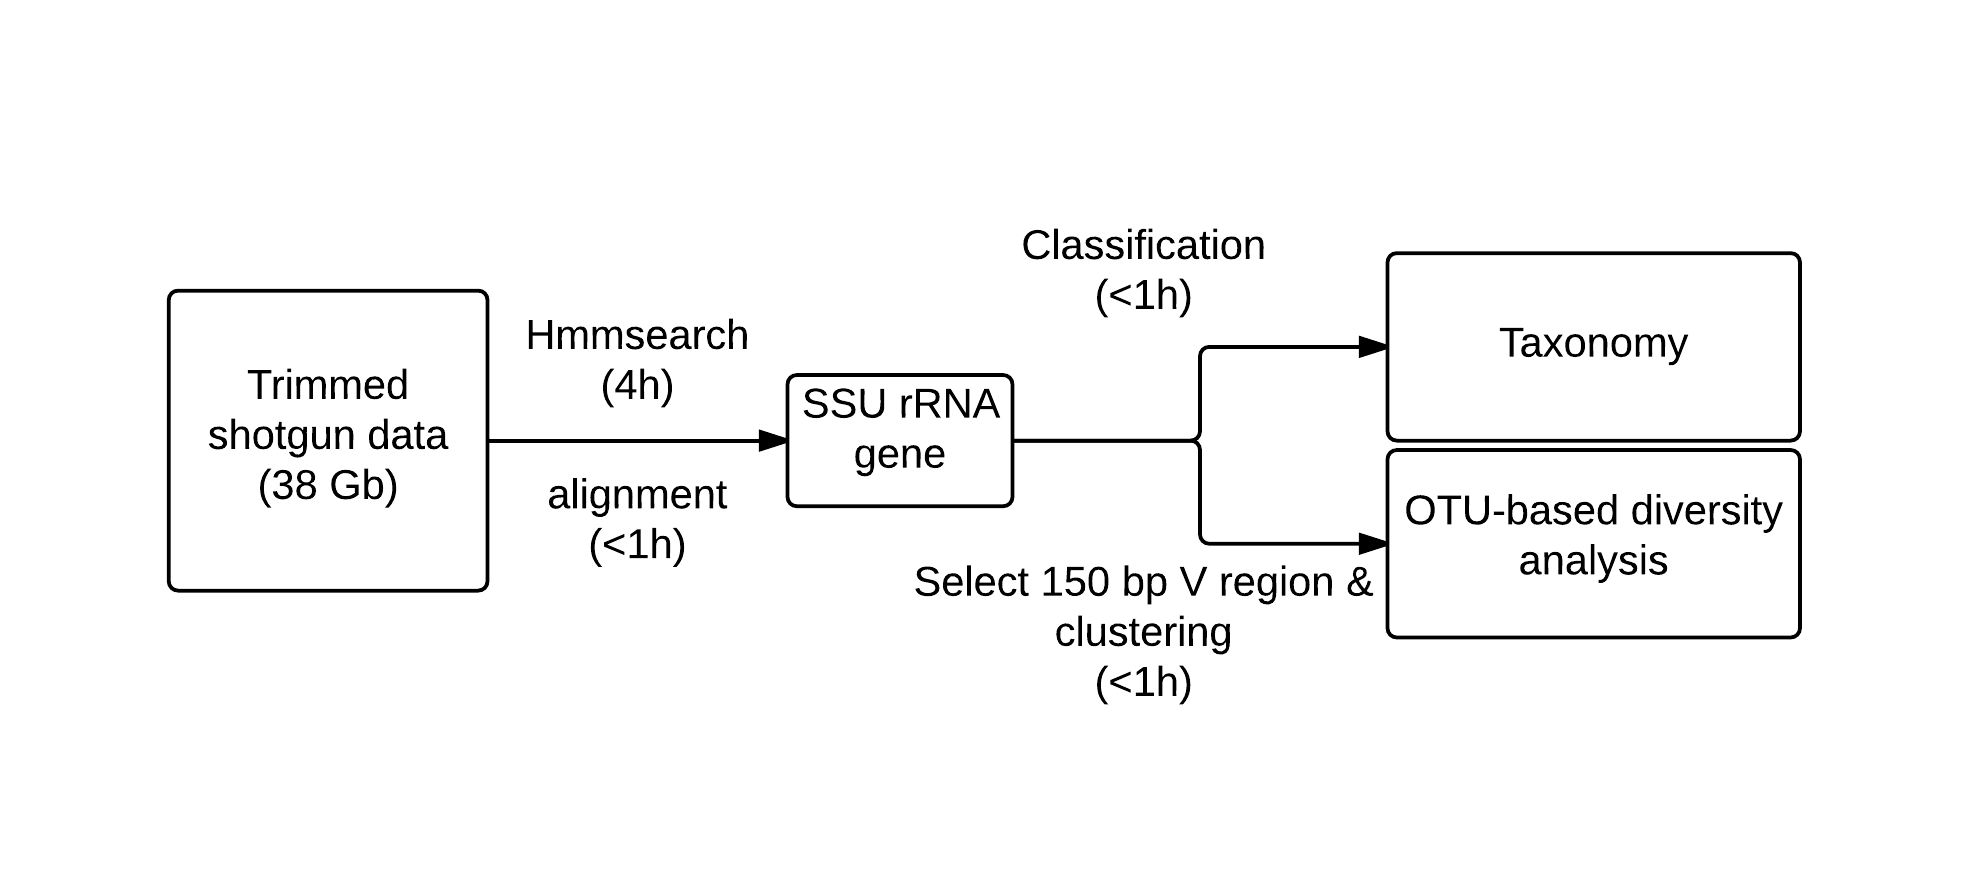
\includegraphics[scale=1]{figs/chap2_figS1}
  \caption[Flowchart of SSUsearch pipeline]{Flowchart of SSUsearch pipeline. SSU rRNA gene fragments were retrieved by an hmmsearch and alignment step, which could be further used for reference-based (supervised) diversity analysis (taxonomy). Those fragments aligned to 150 bp of a variable region could be used for OTU-based (unsupervised) diversity analysis. SSU rRNA gene identification hmmsearch is the most time consuming steps. For 1 lane of trimmed HiSeq data (38 Gb) from Miscanthus rhizosphere sample (M1), SSU rRNA gene identification took about 4 hours with peak memory usage of about 4.5 Gb. In the analysis pipeline, where there was not a clear performance difference between tools, we mostly used Mothur including databases. For (de novo) OTU based analysis, SSU rRNA gene reference sequences with taxonomy information are required for classification. Another smaller set of aligned references is required to align the gene fragments from shotgun data. The SILVA database (the official one, not the one included with QIIME or Mothur) was used to build the HMM since the reference set from SILVA was more up to date. Two scripts in QIIME were used to cluster (UCLUST, the default) and pick representative sequences. Building the HMM is not part of the pipeline but using the built HMM is. We found that complete-linkage clustering is faster and requires less memory with McClust than with Mothur (dist.seqs and cluster). Additionally, we use two scripts in QIIME (pick\_otus.py and pick\_rep\_set.py) to select representative sequences for building the HMM due to ease of use and the GreenGenes database is included for use with the Copyrighter copy number correction tool.}
  \label{fig:chap2FigS1}
\end{figure}


\begin{table}[htbp]
  \centering
  \caption[Comparison of search results from SSUsearch, metaxa and meta-rna]{Comparison of search results from SSUsearch, metaxa and meta-rna. Subsets of 5 million reads from metagenome of a synthetic community of 48 Bacteria and 16 Archaea, SB1 (bulk soil metagenome) and M1 (Miscanthus rhizosphere metagenome) are used as testing data. Symbol ``+'' indicates overlap.}
    \begin{tabular}{|r|r|r|r|}
    \toprule
          & Mock  & SB1   & M1 \\
    \midrule
    SSUsearch & 6432  & 2789  & 2612 \\
    Metarna & 6455  & 2781  & 2600 \\
    Metaxa & 5322  & 2649  & 2444 \\
    \multicolumn{1}{|l|}{SSUsearch+metarna} & 6300  & 2759  & 2576 \\
    \multicolumn{1}{|l|}{SSUsearch+metaxa} & 5286  & 2642  & 2442 \\
    \multicolumn{1}{|l|}{metarna+metaxa} & 5304  & 2649  & 2436 \\
    \multicolumn{1}{|l|}{SSUsearch+metarna+metaxa} & 5268  & 2642  & 2435 \\
    \midrule
    \midrule
    SSUsearch cpu time (min) & 1.6   & 4     & 4.8 \\
    Meta-rna cpu time (min) & 8.6   & 16.5  & 16.9 \\
    Metaxa cpu time (min) & 17.5  & 47.2  & 34.8 \\
    \midrule
    \midrule
    SSUsearch memory (Mb) & 35    & 33    & 30 \\
    Meta-rna memory (Mb) & 3406  & 4005  & 4234 \\
    Metaxa memory (Mb) & 452   & 456   & 572 \\
    \bottomrule
    \end{tabular}%
  \label{tab:chap2Tab1}%
\end{table}%


Unsupervised OTU analysis with shotgun data is not available in any current pipeline and we develop a method for OTU clustering around a small region where all reads overlap. To show the validity of our unsupervised method, we did tests on effects of target region sizes and different variable regions with shotgun data from a synthetic community. We found all region sizes from 50 bp to 160 bp in V4 had an OTU number that approached the species number at a distance cutoff of 4\% or 5\% (\cref{fig:chap2FigS2}) when testing target region size effect on OTU number. We also did a similar test with only full length SSU rRNA genes from 64 species to make sure OTU number is close to species number and confirmed that OTU number was close to species number (at a range from 50 to 60) when a cutoff of 0 to 0.06 was chosen (\cref{fig:chap2FigS3}). When target region size was larger than 170 bp, the clustering tool (McClust) \cite{cole_ribosomal_2014} did not cluster because percentage of non-overlapping reads exceeded its threshold. Based on the above results, we chose 80 bp or 120 bp as the target region size and 5\% distance cutoff for testing different hyper variable regions. The number of OTUs created in all variable regions is close to the real number of species in the synthetic community except when using V3.


\begin{figure}[tbph!]
  \centering
  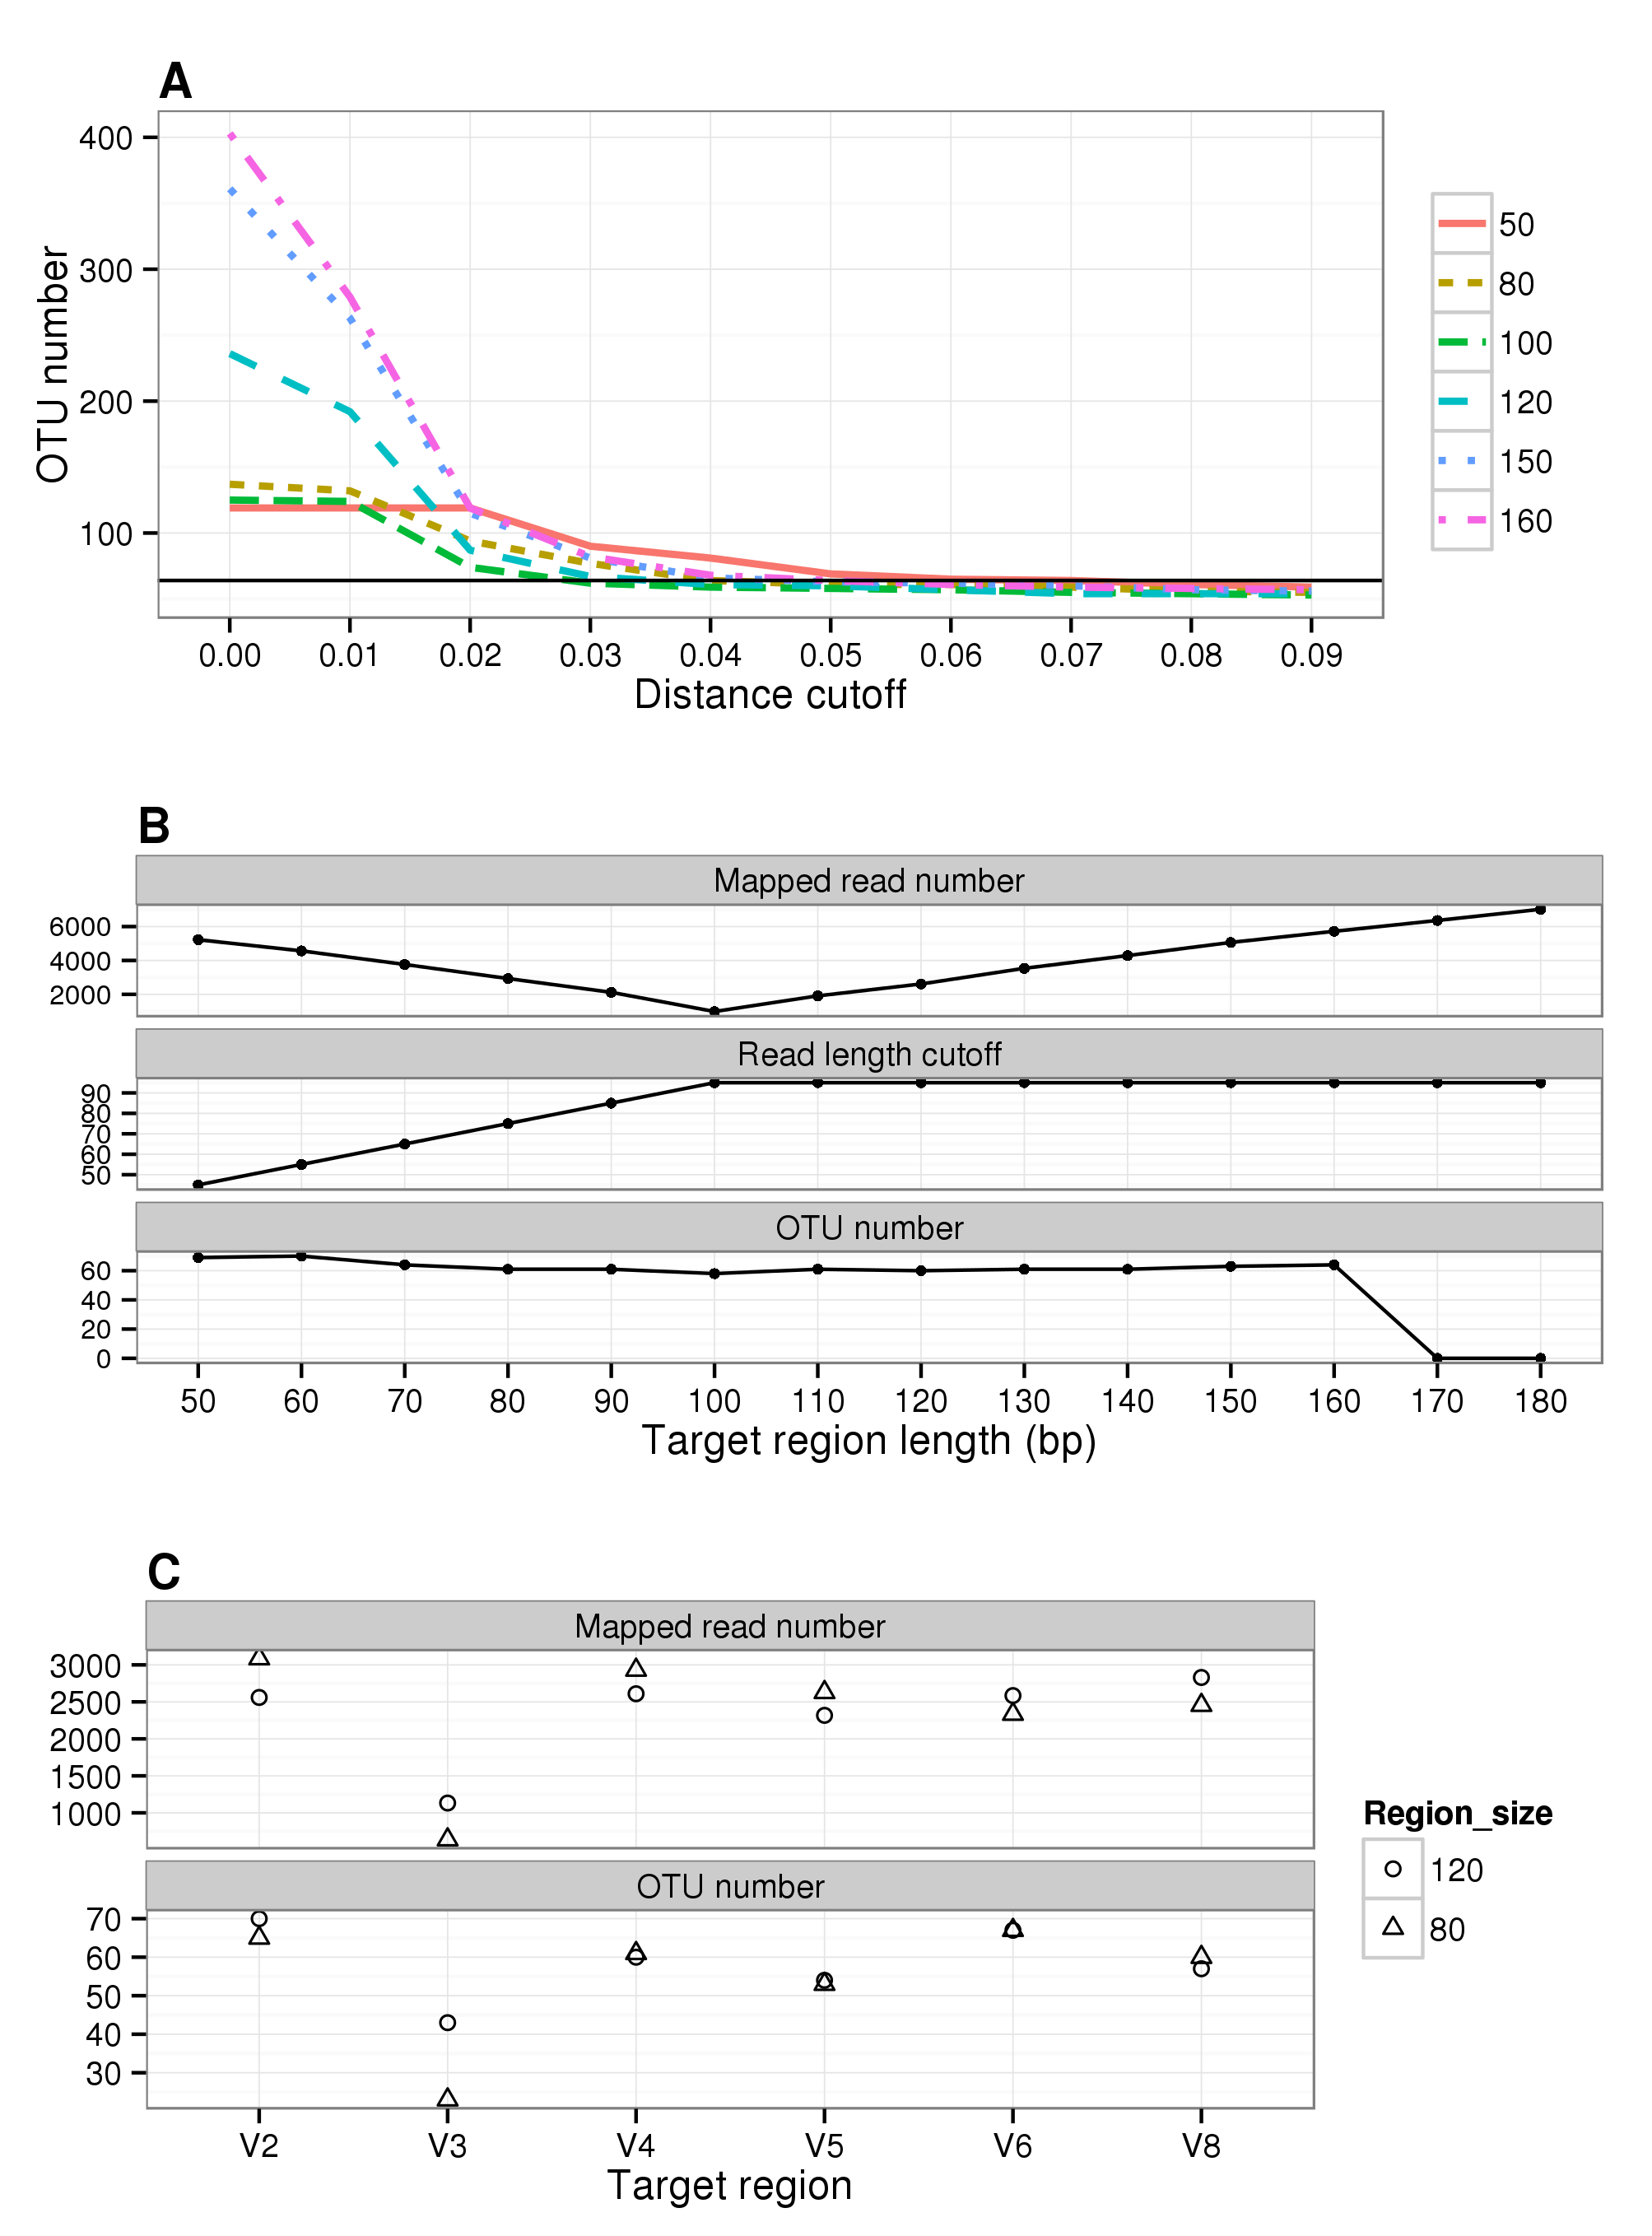
\includegraphics[width=0.60\textwidth]{figs/chap2_figS2}
  \caption[Testing the effect of target region size and variable region on clustering on a synthetic community]{Testing the effect of target region size and variable region on clustering on a synthetic community with 64 species with read length at about 100 bp. Subfigure A shows a distance cutoff of 4\% or 5\% is proper for all regions sizes from 50 bp to 160 bp in V4 (OTU number approached the species number 64 as indicated by the black line).  Subfigure B shows more details in the method used for subfigure A. Panel “Read Length cutoff” in B shows minimum read length was set to the target region size minus 5 bp if the region size was less than 100 bp, and 95 bp when the region size was longer than 100 bp. As a result, the number of reads aligned decreased as the target region size increased until 100 bp, and then the number of reads aligned increased with target region as shown in Panel “Mapped read number” in B. Panel “OTU number” in C shows OTU number at distance cutoff of 0.05 and our method works well from a 50 bp region to 160 bp region in V4. Subfigure C tests our unsupervised method on multiple hyper-variable regions (V2, V3, V4, V5, V6, V8) with region size of 120 bp (circle) and 80 bp (triangle). Panel “Mapped read number” in C shows the number of reads mapped to each chosen region. Panel “OTU number” in C shows the number of OTUs in each region at distance cutoff of 0.05. All regions have consistent mapped read number and OTUs except V3.}
  \label{fig:chap2FigS2}
\end{figure}


\begin{figure}[tbph!]
  \centering
  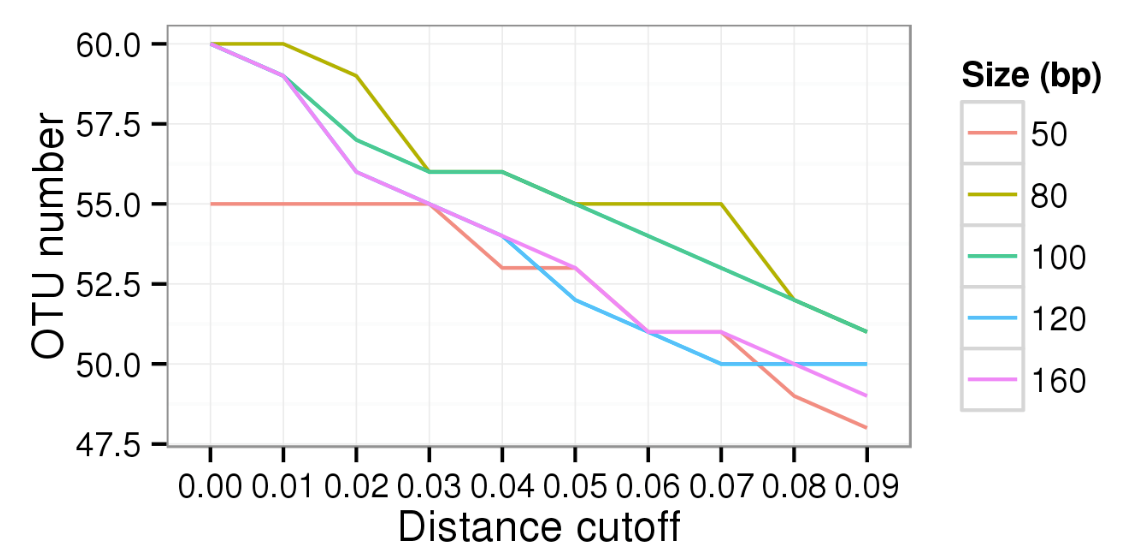
\includegraphics[width=0.80\textwidth]{figs/chap2_figS3}
  \caption[Testing the effect of target region size on V4 of full-length SSU rRNA genes from a synthetic community]{Testing the effect of target region size on V4 of full-length SSU rRNA genes from a synthetic community with 64 species.}
  \label{fig:chap2FigS3}
\end{figure}


Reproducibility between technical replicates is important and a basic feature of a method \cite{zhou_reproducibility_2011,zhou_high-throughput_2015}. We evaluated it by comparing the correlation of OTU abundance between technical replicates from the bulk soil sample and found high correlation between them (Pearson’s correlation coefficient = 0.997). The consistency was better for the more abundant OTUs (\cref{fig:chap2FigS4}A). Log transformation could reduce the effect of high abundance OTUs on the overall correlation. Even with log-transformed abundance, the two replicates have a Pearson’s correlation coefficient of 0.91 and linear regression R2 of 0.88 when OTUs with less than 25 total counts were discarded (\cref{fig:chap2FigS4}B). The choice of 25 cutoff was chosen to compare to another study on amplicon reproducibility \cite{lundberg_defining_2012} and as mentioned in the Discussion. 

\begin{figure}[tbph!]
  \centering
  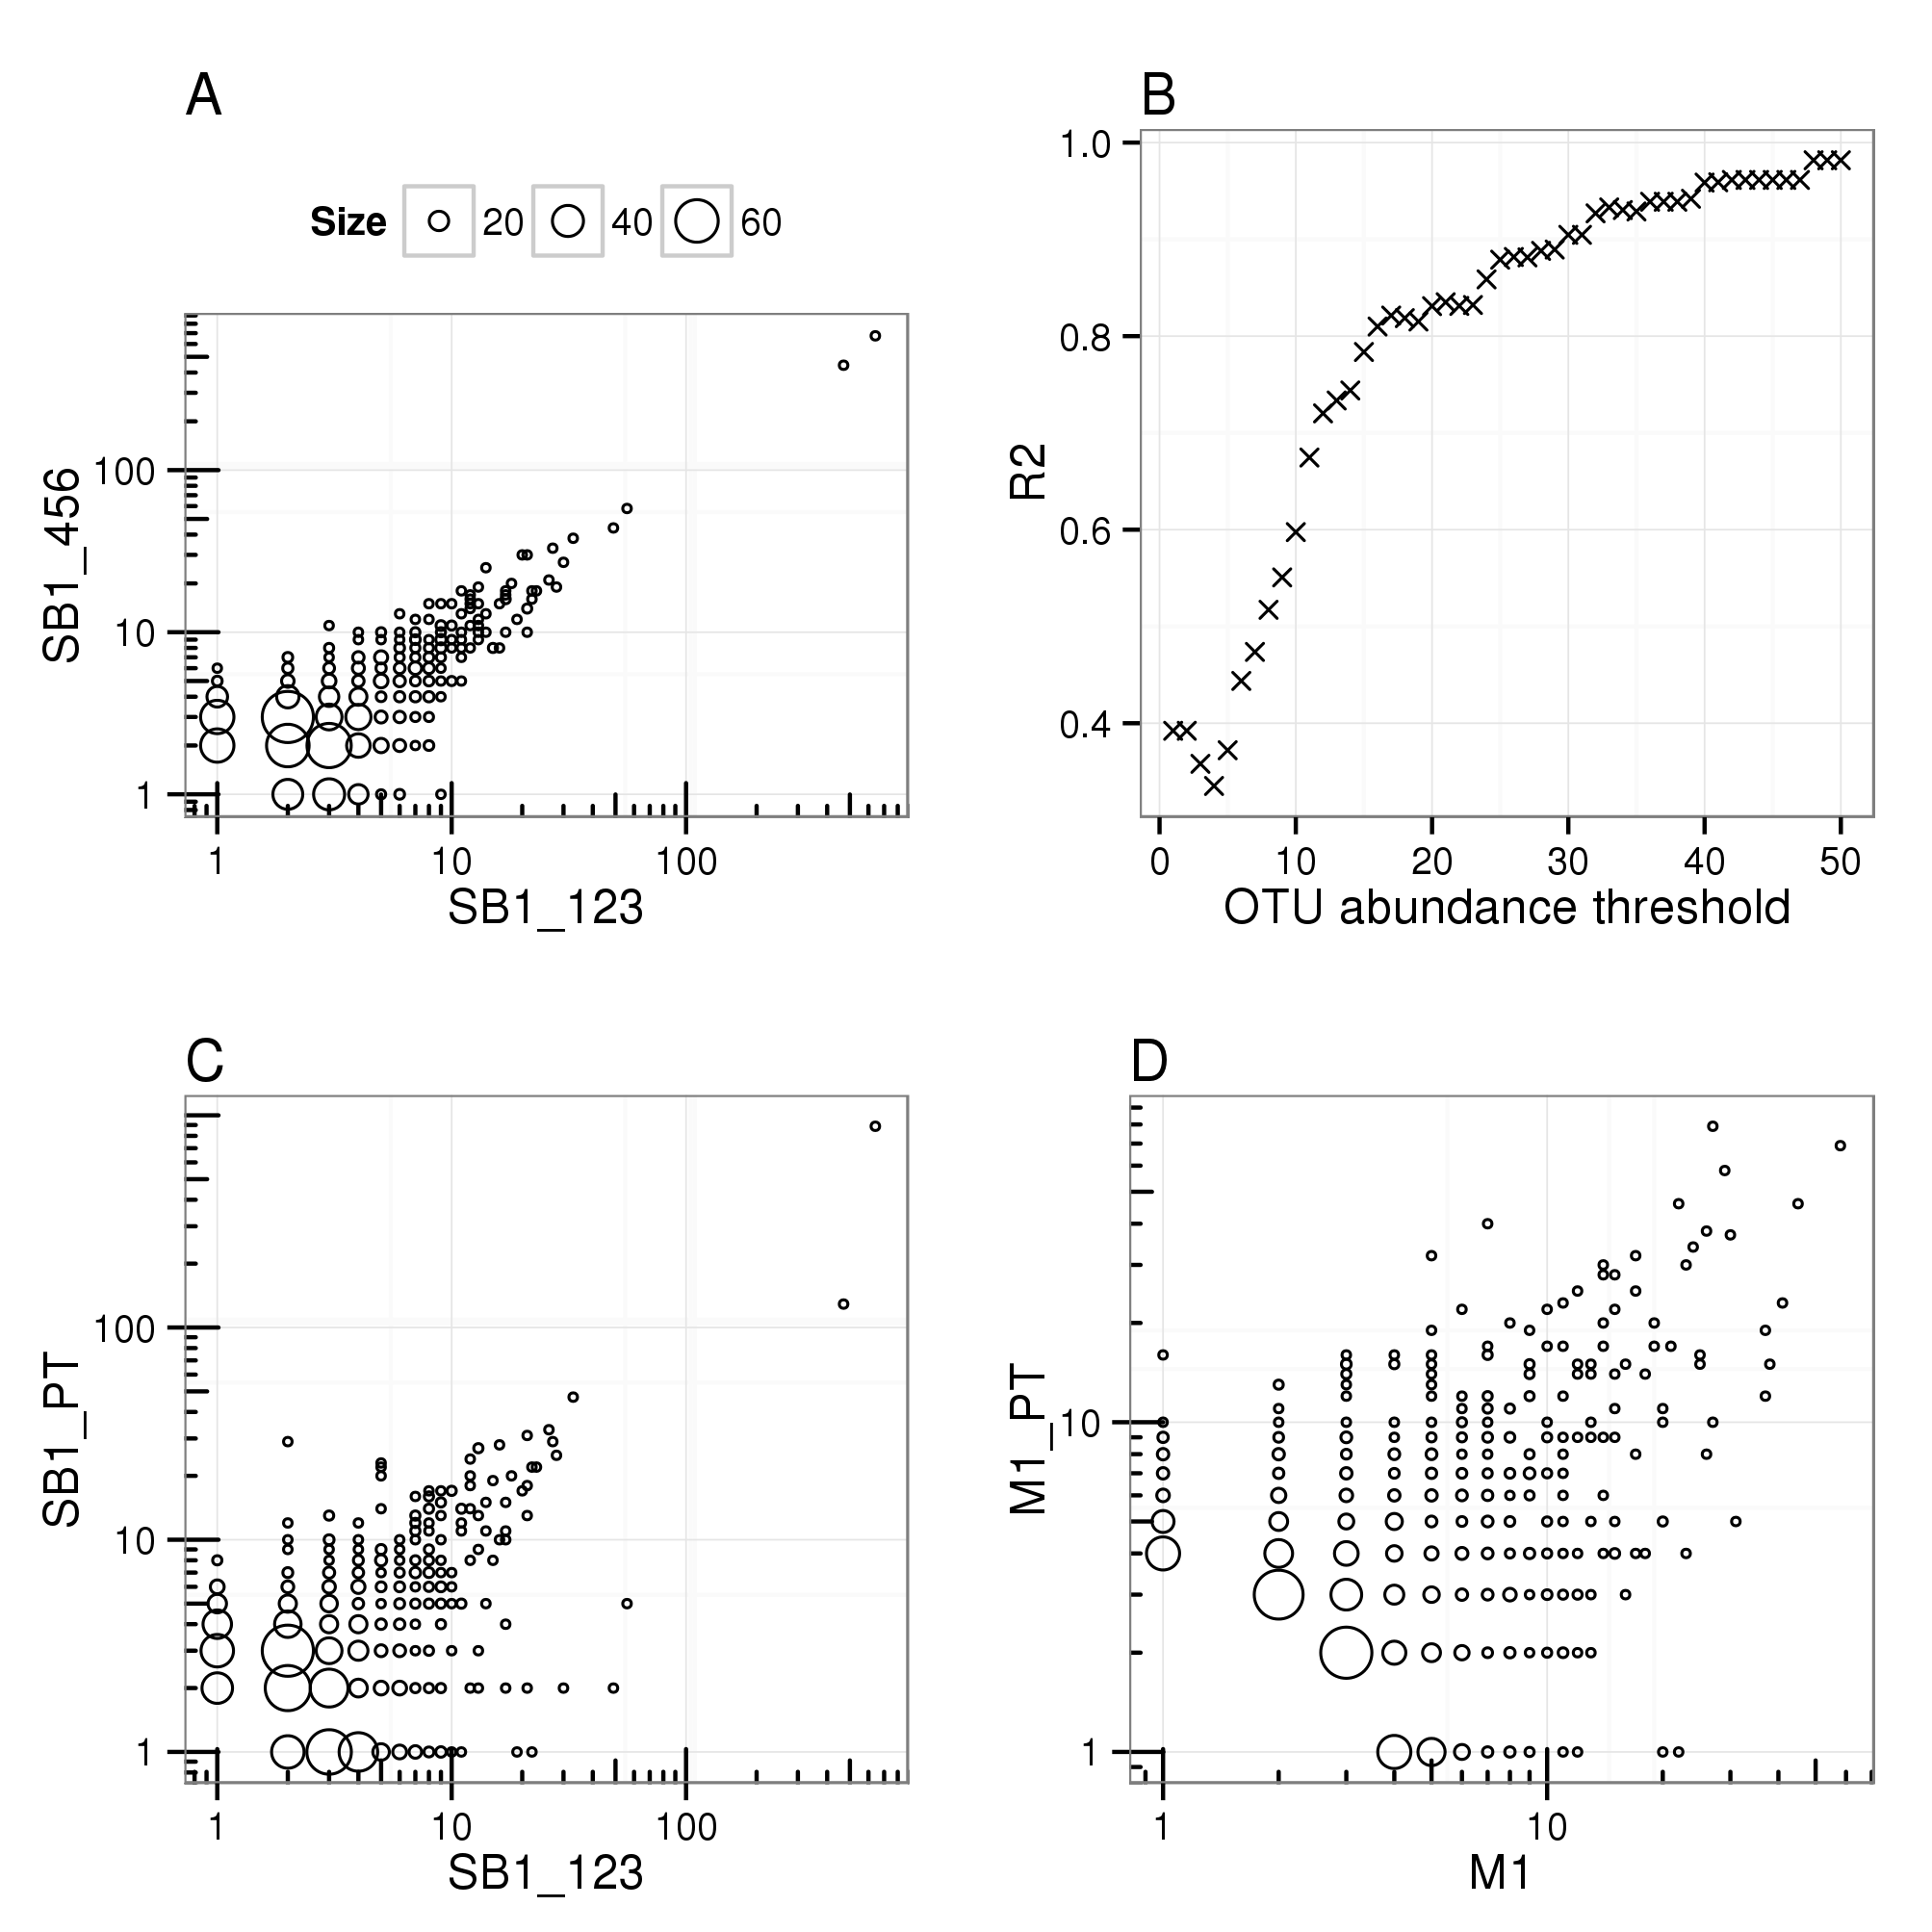
\includegraphics[width=0.60\textwidth]{figs/chap2_figS4}
  \caption[Technical reproducibility test and comparison of OTU abundances between paired shotgun and amplicon data]{Technical reproducibility test of our unsupervised clustering and comparison of OTU abundances between paired shotgun and amplicon data. Subfigure A shows consistent OTU abundance profiles in two technical replicates (Pearson’s correlation coefficient is 0.997). X axis shows number of reads in each OTU in replicate SB1\_123, and y axis shows number of reads in each OTU in replicate SB1\_456. The size of circle is proportional to number of OTUs at the same location in the plot (with the same counts in SB1\_123 and also in SB1\_456).  The consistency of counts of each OTU in two replicates becomes better when the abundance of OTUs are higher. Subfigure B shows progressive dropout analysis of two technical replicates of shotgun data. There is significant correlation of counts of each OTU between technical replicates; X axis is the threshold of OTU abundance and y axis is the R2 of linear regression of log transformed OTU abundances in two replicates. OTUs with lower abundance than the thresholds (x axis) were discarded before regression analysis. Subfigure C and D shows comparison of OTU abundance profile between paired shotgun and amplicon data in bulk soil sample (SB1) and rhizosphere sample (M1), respectively. There is inconsistency between shotgun data and amplicon data in both samples. X axis shows number of SSU rRNA gene fragments in shotgun data per OTU in log scale, and y axis shows number of amplicon sequences in each OTU in log scale. The OTU abundance in both amplicon and shotgun data were increased by 1 to avoid 0 counts that can be displaced in log scale. The size of circle is proportional to number of OTUs with the same abundance in both types of data. There are OTUs with significantly different abundances in the two types of data (circles deviate from diagonal line). Pearson’s correlation between two types of data is 0.873 in SB1 and 0.581 in M1.}
  \label{fig:chap2FigS4}
\end{figure}


We also compared OTU-based microbial community structures inferred from shotgun and amplicon SSU rRNA gene sequences. OTU abundances in shotgun and amplicon data, however, do not correlate as well (Pearson’s correlation coefficient of 0.87 for the bulk soil sample SB1 (\cref{fig:chap2FigS4}C) and 0.58 for the Miscanthus rhizosphere sample M1 (\cref{fig:chap2FigS4}D), showing that the amplicon and shotgun methods are not providing the same information. The classification of OTUs with total abundance higher than 10 and with ratio between two data type higher than five fold shows Verrucomicrobia were biased against in the bulk soil sample (SB1\_PT) amplified by V6-V8 primer, while they were biased to in the rhizosphere sample (M1\_PT) amplified by V4 primer. Actinobacteria was biased against in M1\_PT amplified by V4 primer (\cref{fig:chap2FigS5}).  The above results were consistent with the taxonomy-based comparison of the two data types (see below) that suggesting primer bias in amplicon data.


\begin{figure}[tbph!]
  \centering
  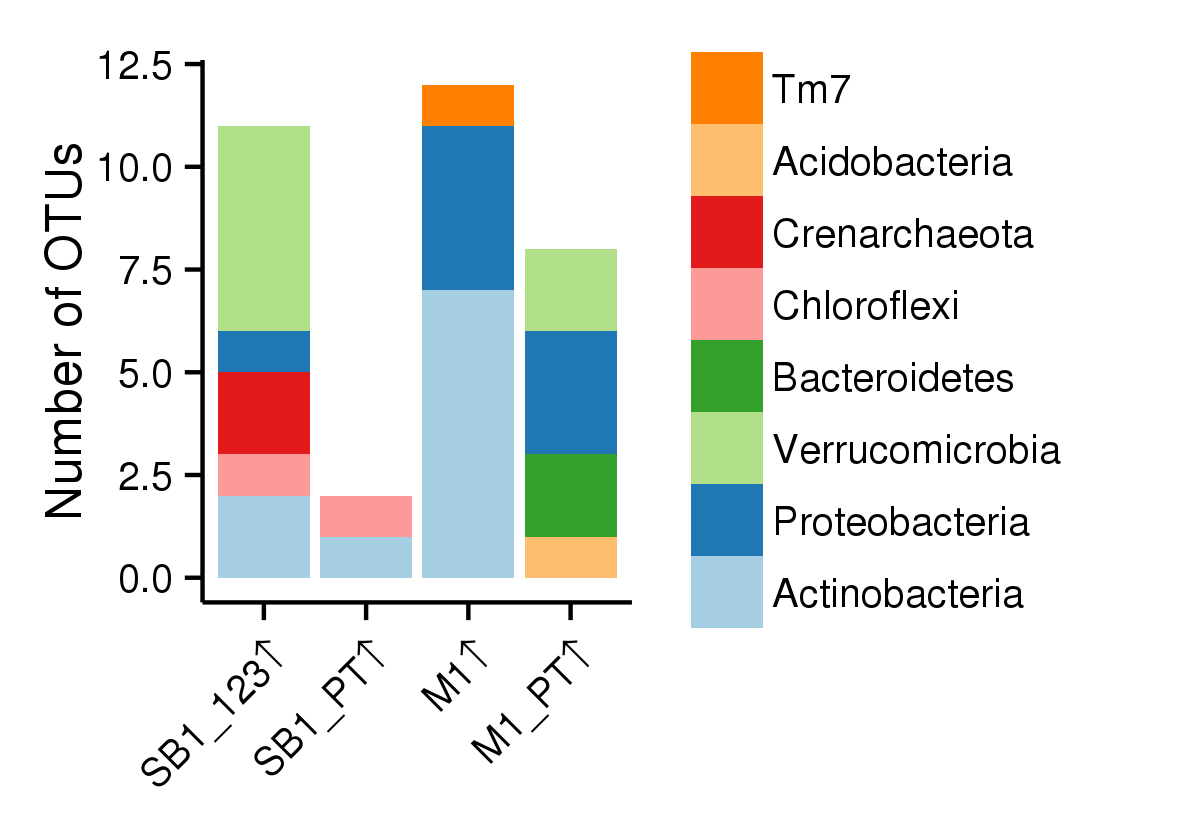
\includegraphics[scale=1]{figs/chap2_figS5}
  \caption[Phyla of OTUs significantly different between shotgun data and amplicon data]{Phyla of OTUs significantly different between shotgun data and amplicon data. SB\_123 are shotgun data and SB1\_PT are amplicon data both from the same DNA from bulk soil sample. M1 are shotgun data and M1\_PT are amplicon data both from the same DNA from Miscanthus rhizosphere sample. OTUs significantly different were defined as those with total abundance > 10 and fold change between two types of data > 5 or < 0.2. Verrucomicrobia was biased against in bulk soil sample amplified by V6-V8 primer (SB1\_PT) but biased for in rhizosphere sample amplified with V4 primer (M1\_PT). Actinobacteria was biased against in rhizosphere sample (M1).}
  \label{fig:chap2FigS5}
\end{figure}


We applied ordination analysis to OTU tables from unsupervised analysis of corn and Miscanthus rhizosphere samples. OTUs from shotgun and amplicon data both showed separation of rhizosphere communities of corn and Miscanthus (horizontal dimension in \cref{fig:chap2Fig1}), as well as a significant difference between the two data types (vertical dimension in \cref{fig:chap2Fig1}), confirming the difference between shotgun and amplicon data. Significant separation (p < 0.001 by AMOVA test in Mothur) of corn and Miscanthus samples was also observed when V2, V4, V6, and V8 shotgun data were used for clustering (\cref{fig:chap2Fig2}) but the sample groupings were the same for all variable regions. \Cref{fig:chap2Fig1,fig:chap2Fig2} showed that the dispersion among the seven corn replicates was much higher than for the Miscanthus replicates. Miscanthus samples had higher alpha diversity than corn samples as shown for all of V2, V4, V6 and V8 regions, although there were variations among these regions (\cref{fig:chap2Fig3}).


\begin{figure}[tbph!]
  \centering
  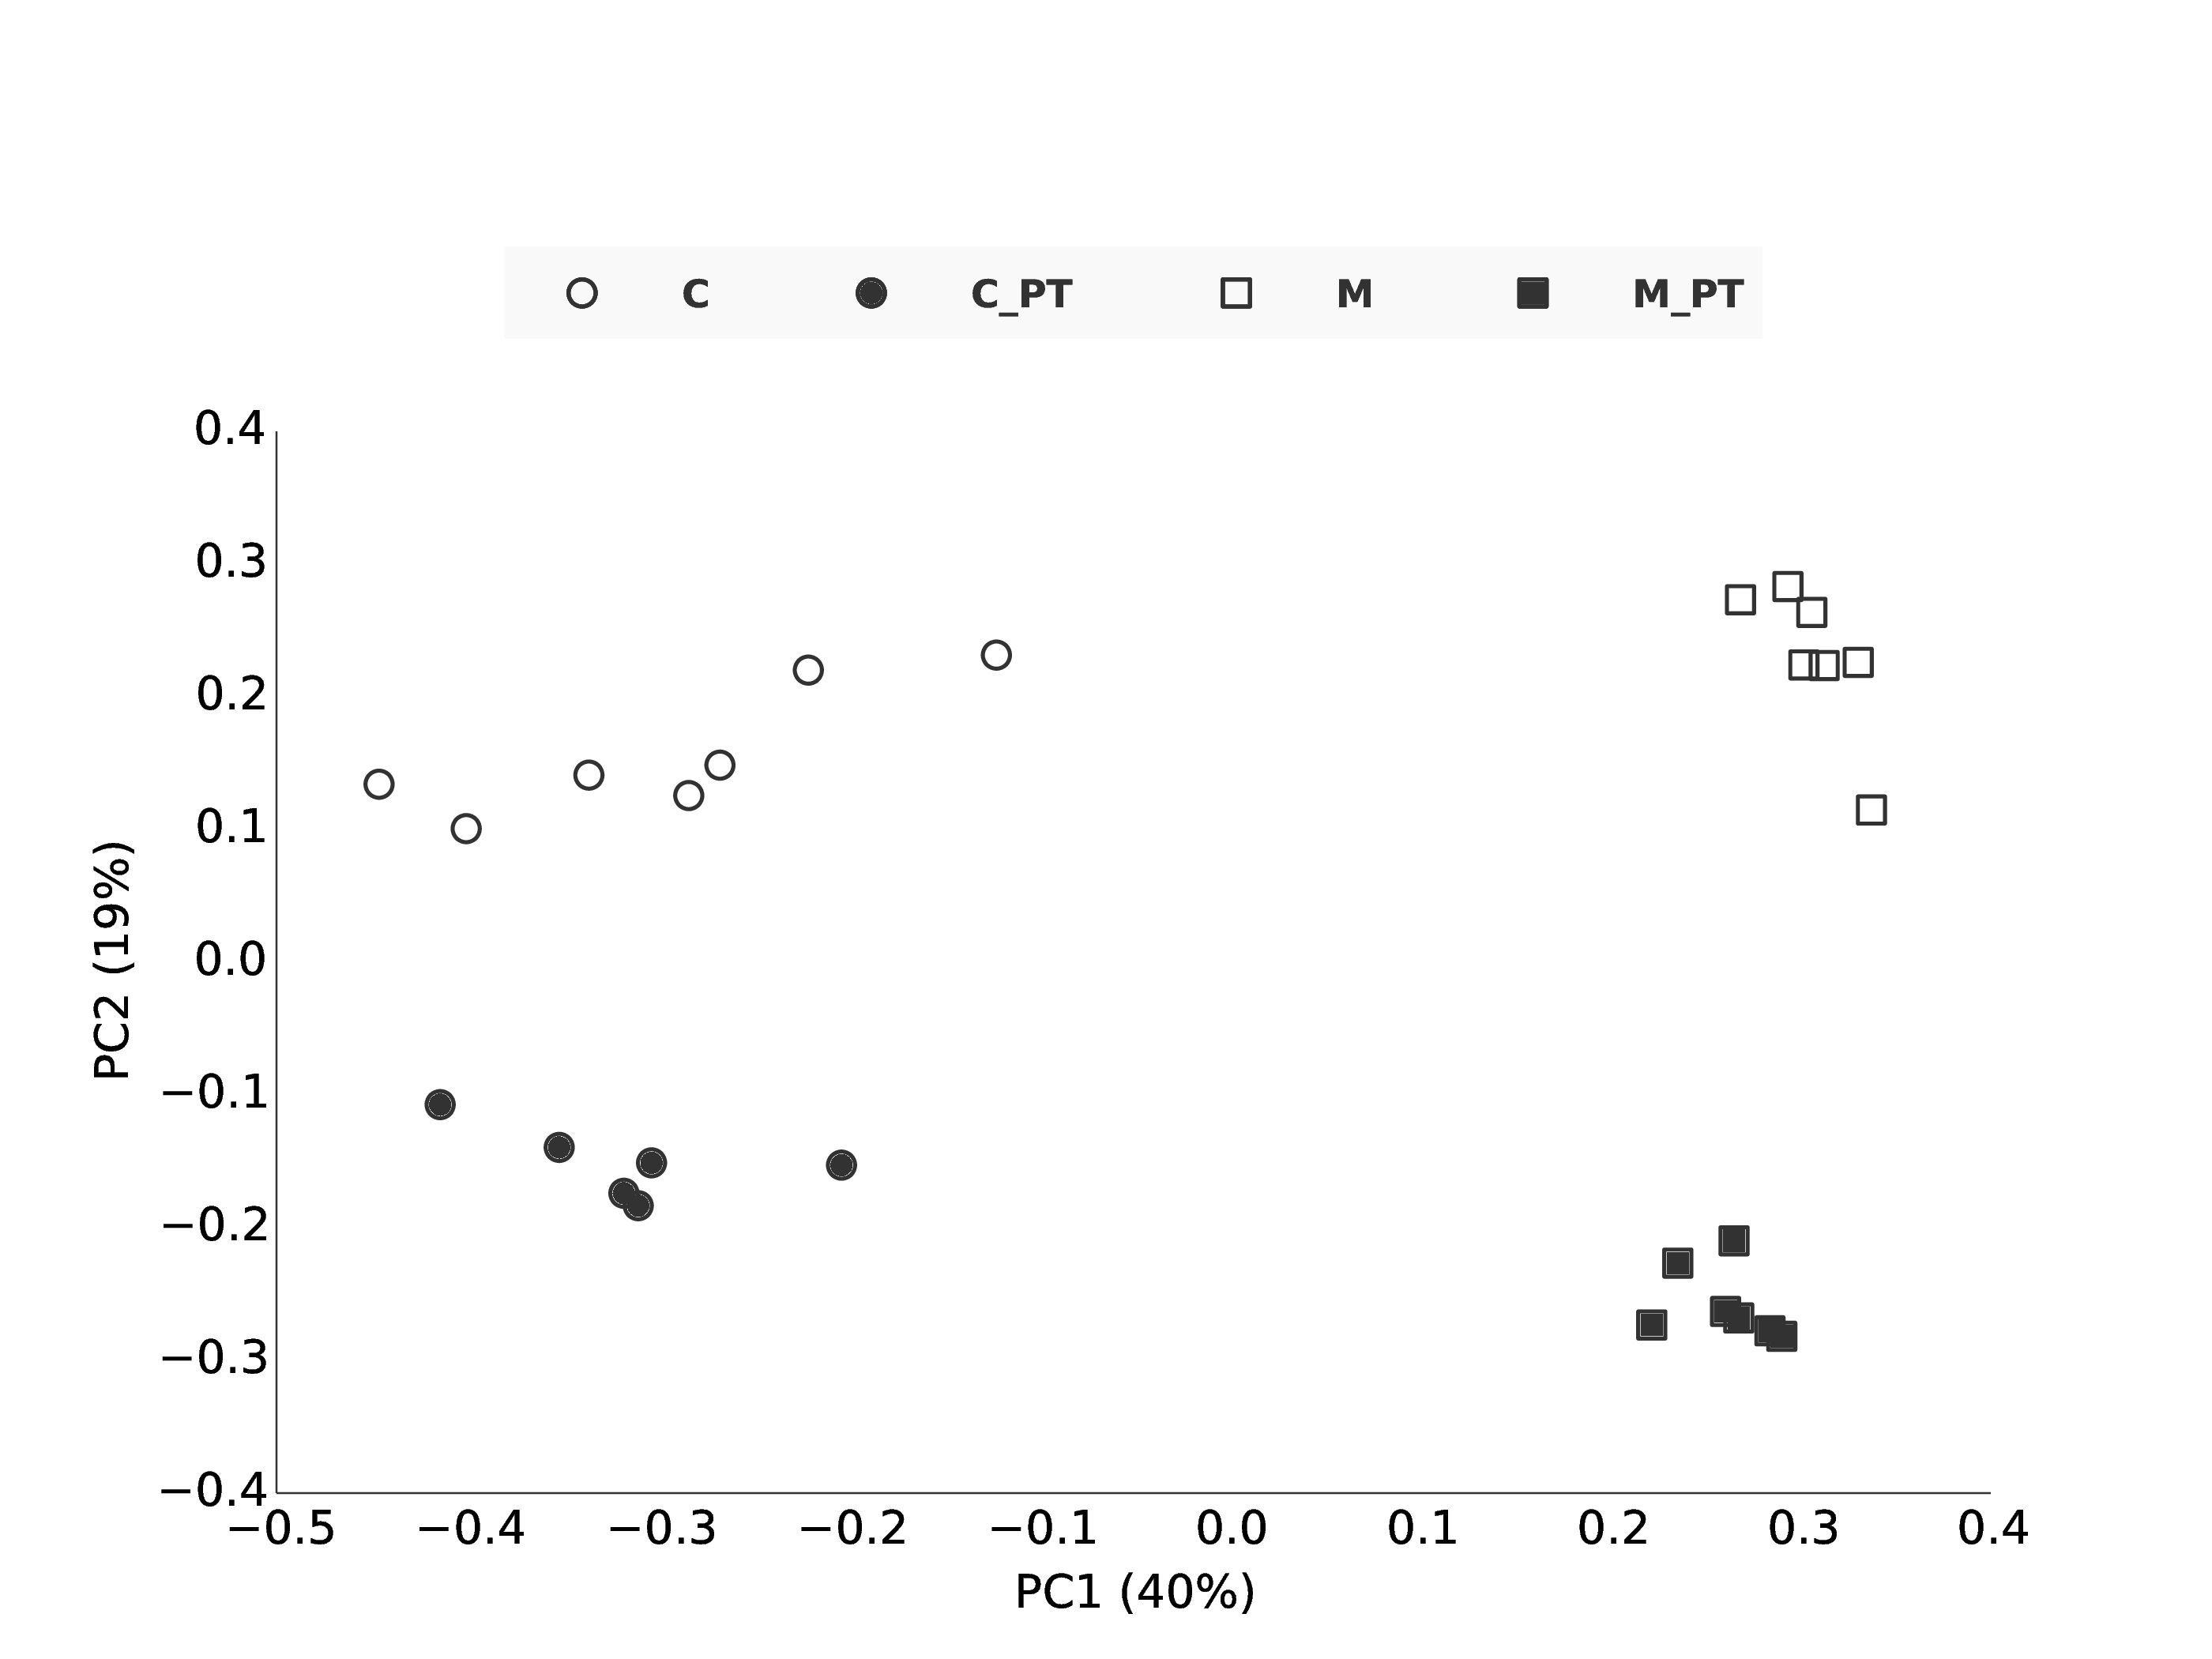
\includegraphics[width=0.80\textwidth]{figs/chap2_fig1}
  \caption[Ordination of amplicon and shotgun data from the same samples]{Principle coordinates analysis (PCoA) of amplicon and shotgun derived data from seven field replicates. There are significant differences between amplicon (filled) and shotgun (unfilled) derived data (along y-axis) and between corn (circle) and Miscanthus (square) rhizosphere samples (along x-axis), (AMOVA p-value < 0.001). PCoA was applied to OTU table resulting from clustering with shotgun data and amplicon data using 150bp of V4 region. Labels with suffix ``\_PT'' are amplicon data and others are shotgun data.}
  \label{fig:chap2Fig1}
\end{figure}


\begin{figure}[tbph!]
  \centering
  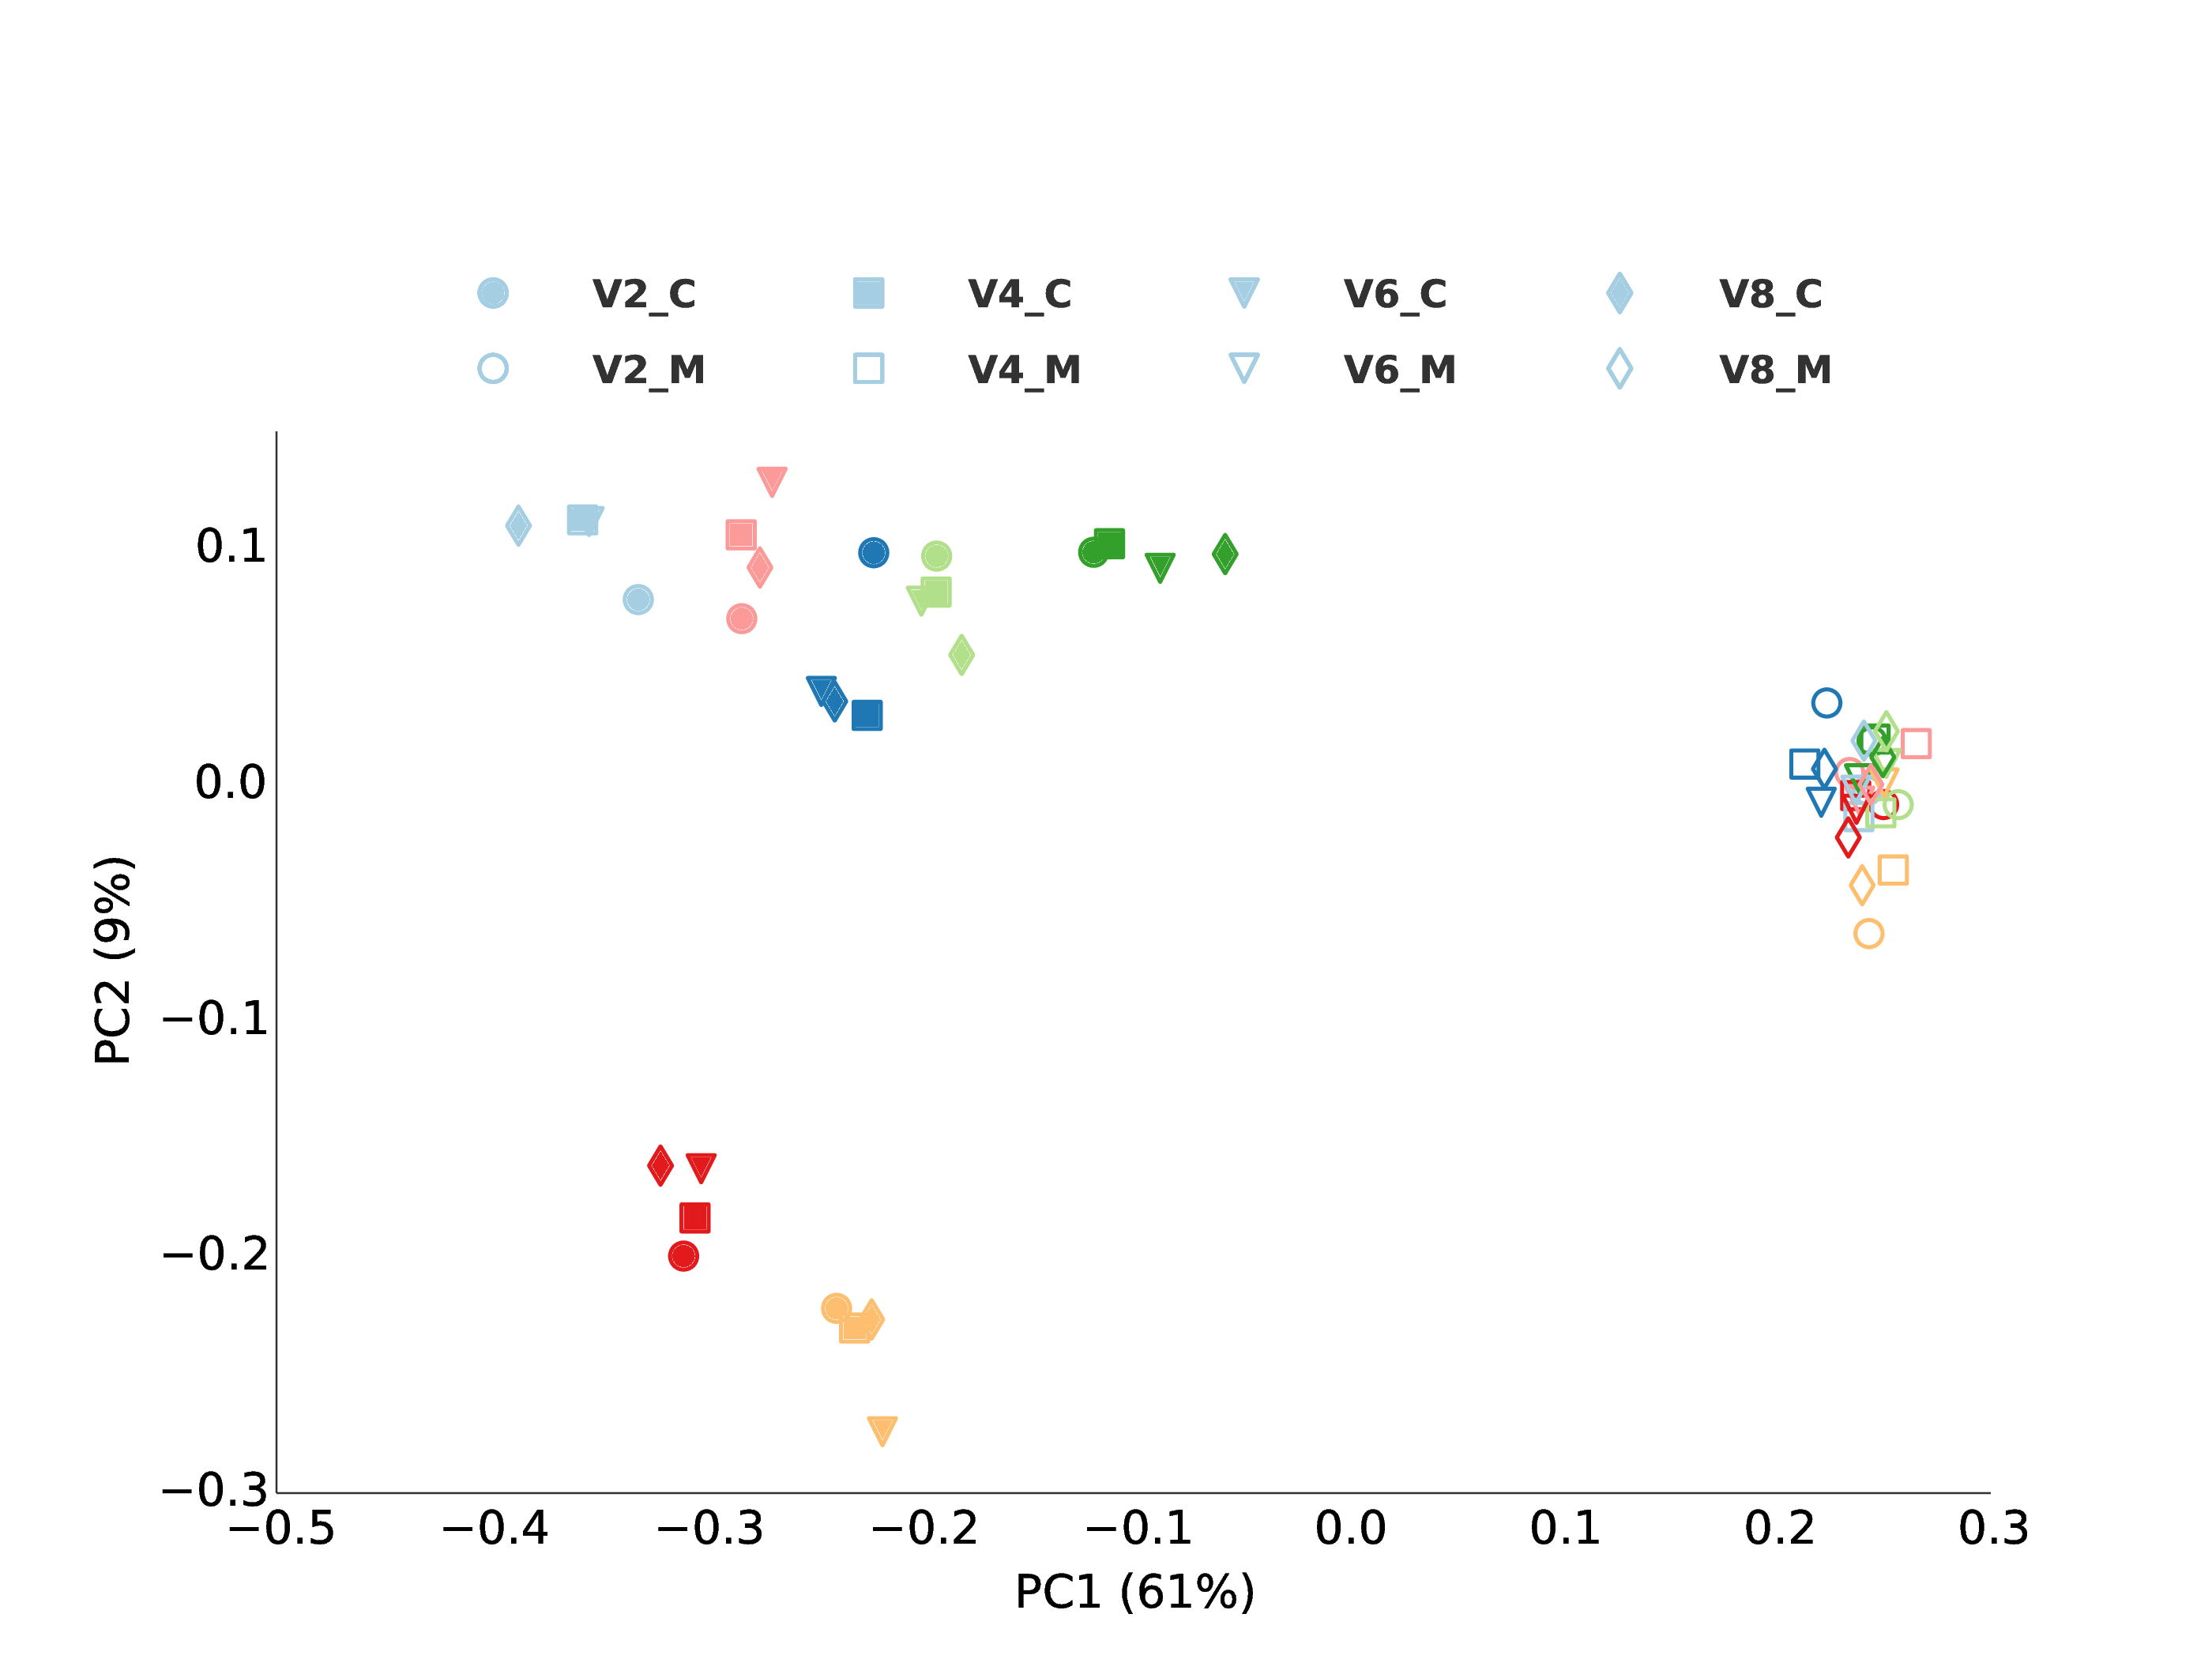
\includegraphics[width=0.80\textwidth]{figs/chap2_fig2}
  \caption[Comparsion of ordination analysis with different variable regions]{Comparsion of ordination analysis with different variable regions. PCoA of OTUs from different SSU rRNA variable regions (V2, V4, V6, and V8) was applied on corn (filled markers, ``\_C'') and Miscanthus (unfilled markers, ``\_M'') rhizosphere samples. Different colors indicate the seven replicates. OTU tables from clustering of shotgun data using 150bp of V2, V4, V6 and V8 regions were used for PCoA and procrustes analysis in QIIME was used to transform the PCoA results from different regions and plot them in the same figure.}
  \label{fig:chap2Fig2}
\end{figure}


\begin{figure}[tbph!]
  \centering
  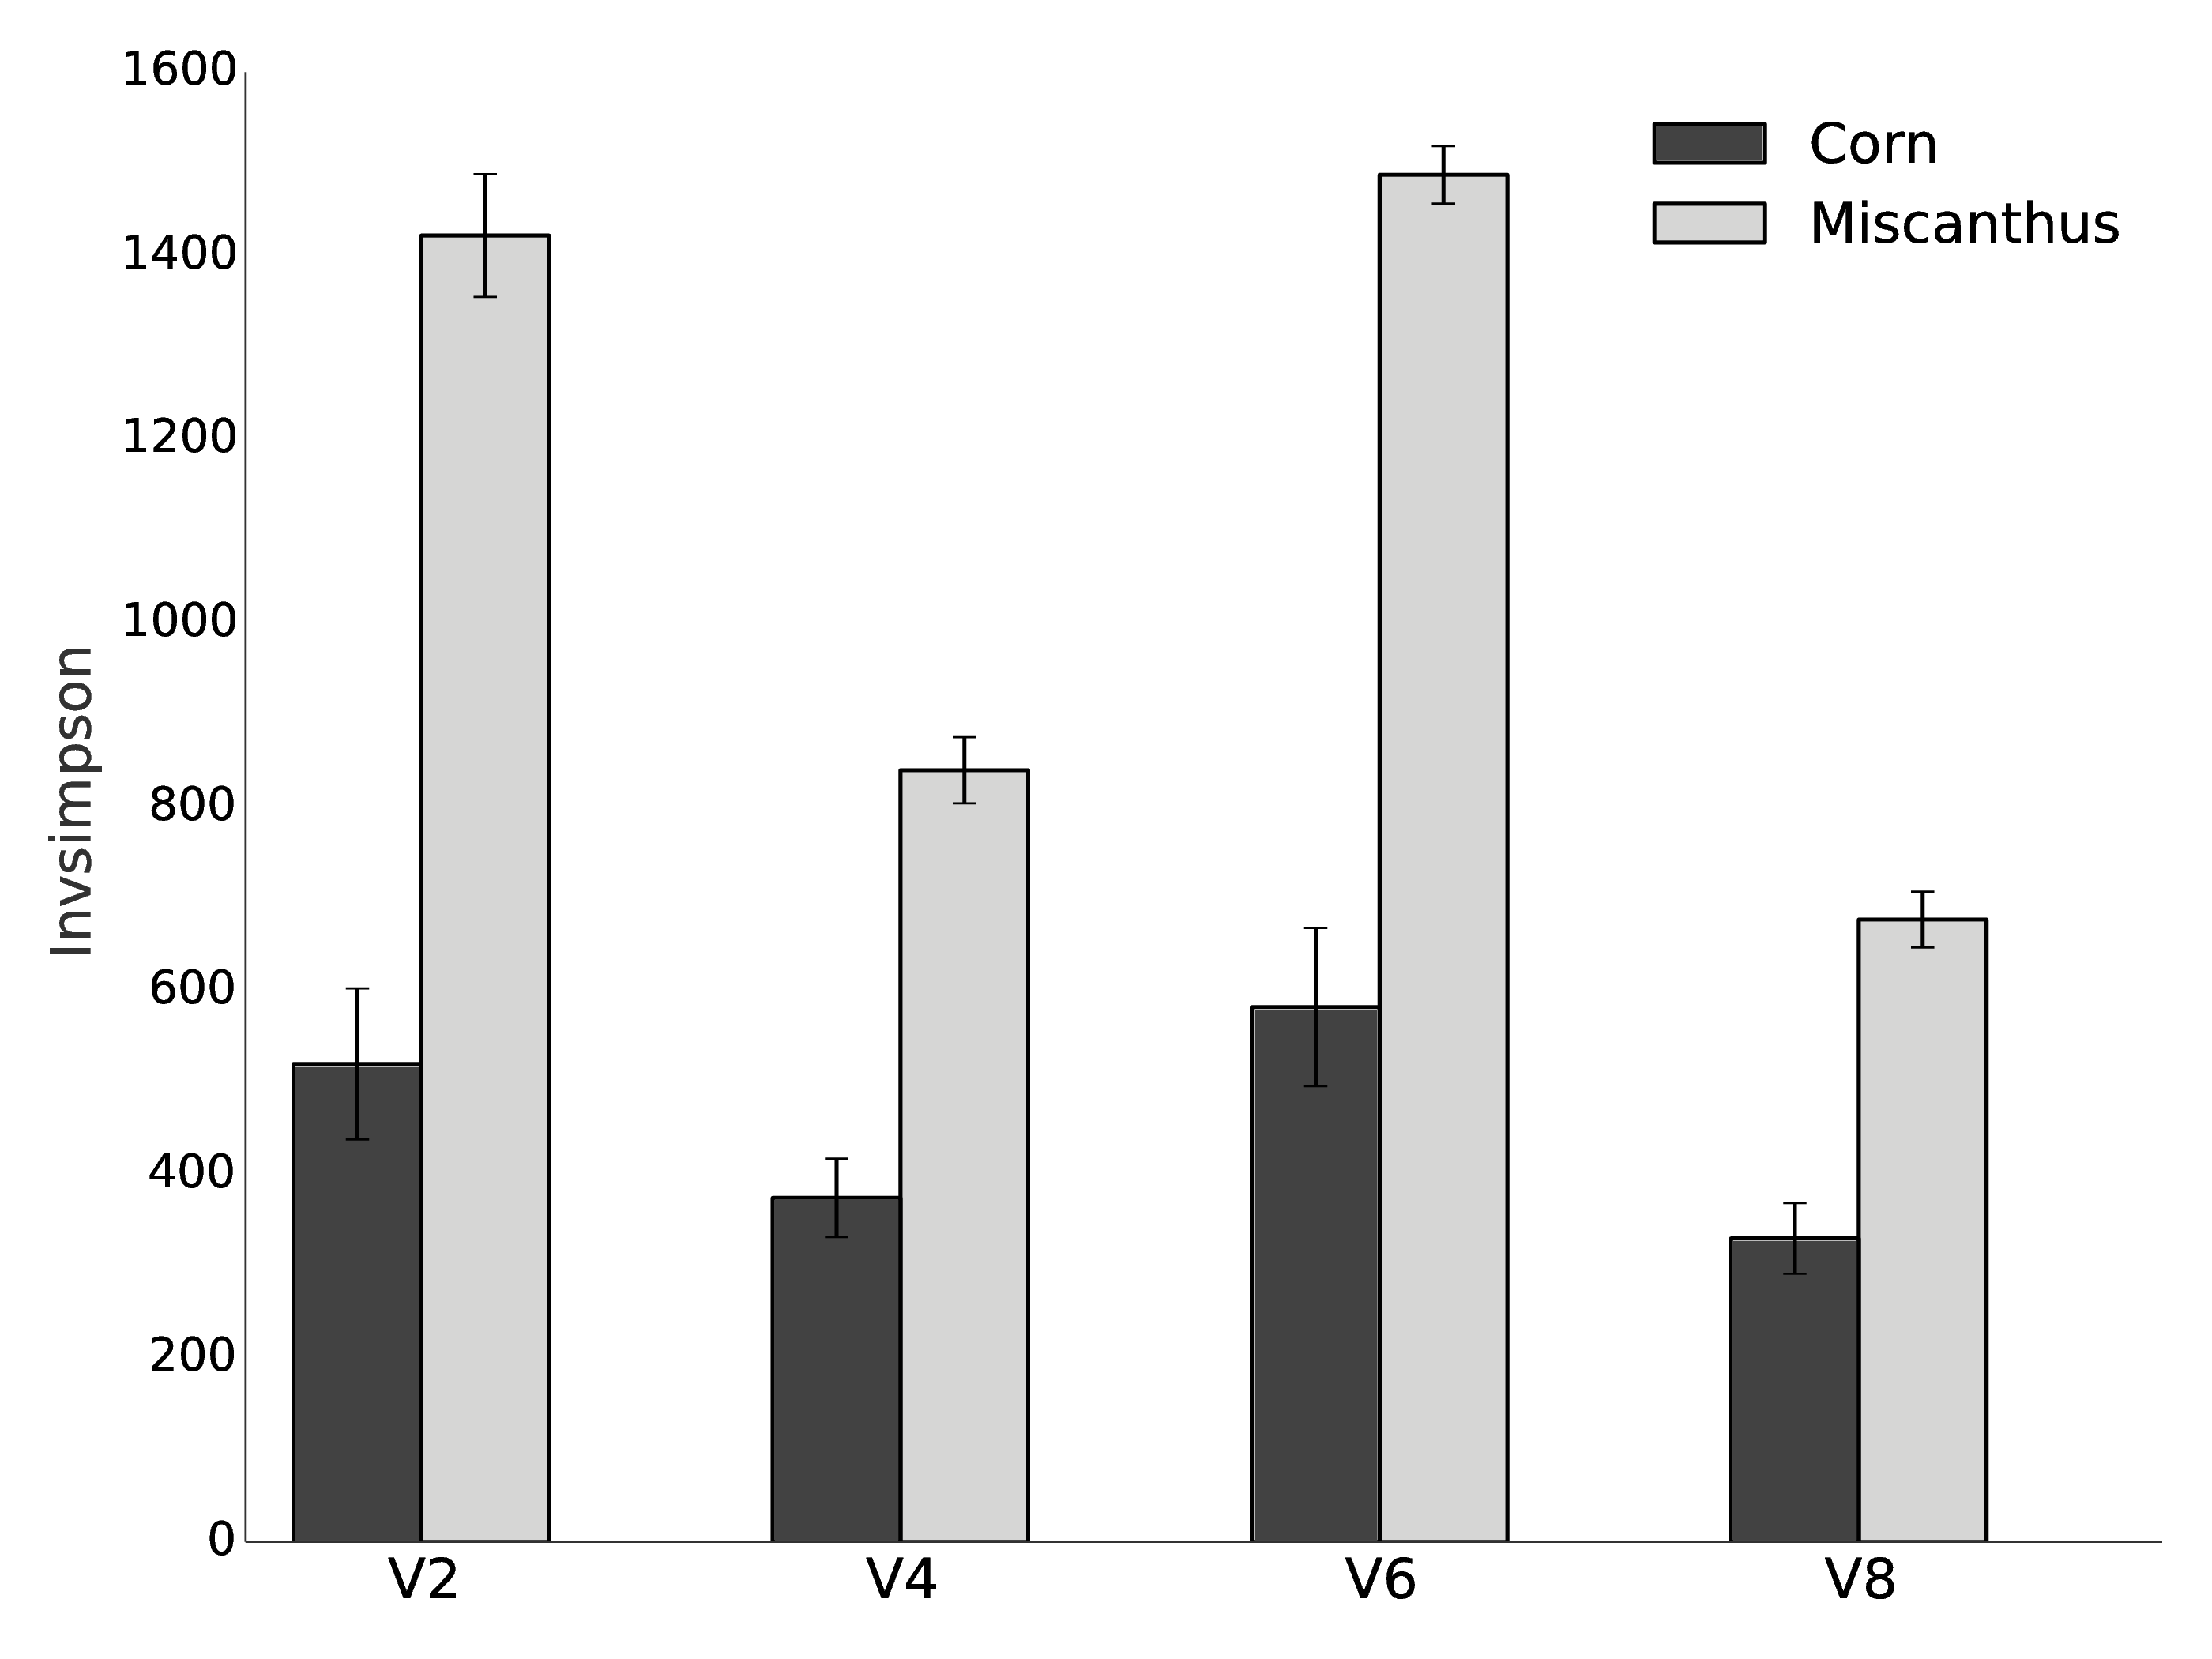
\includegraphics[width=0.80\textwidth]{figs/chap2_fig3}
  \caption[Alpha diversity comparisons between corn and Miscanthus using V2, V4, V6 and V8 regions]{Alpha diversity comparisons between corn and Miscanthus using V2, V4, V6 and V8 regions. All variable regions showed Miscanthus is more diverse than corn, even though there was variation of diversity among rRNA gene regions. Alpha diversity was calculated with inverse Simpson using OTUs resulting from clustering with different variable regions.}
  \label{fig:chap2Fig3}
\end{figure}


We compared the taxonomy-based microbial community structures inferred from shotgun data with those from amplicon SSU rRNA gene sequences (12163 amplicon for SB1 and 60148 for M1) and confirmed known primer biases and revealed a new bias. Before comparing two data types, we looked at the taxonomy profile of shotgun data using different variable regions. Shotgun data mapped to different variable regions shows similar taxonomy at the Bacterial phylum level (Pearson’s correlations > 0.96) except that V6 has more unclassified sequences (\cref{fig:chap2FigS6}). Since different variable regions may provide different taxonomic precision to certain groups \cite{guo_taxonomic_2013}, taxonomy information from all regions may better represent the taxonomy profile. Thus we used all SSU rRNA gene fragments for taxonomy comparison with amplicon data. Both shotgun and amplicon data show Actinobacteria, Proteobacteria and Acidobacteria as the three most abundant phyla, as is expected for soil \cite{janssen_identifying_2006}. Since shotgun data are more accurate on estimating community structure, thus we accept the shotgun data as the reference \cite{haas_chimeric_2011,shakya_comparative_2013}. The 926F/1392R (V6-V8) primer set is biased against Verrucomicrobia (0.3\% in amplicon data vs. 5.8\% in shotgun data by RDP database) in bulk soil sample SB1 (\cref{fig:chap2Fig4}), and the 515F/806R (V4) primer set biased against Actinobacteria (11.6\% in amplicon data vs. 26.6\% in shotgun data) and towards Verrucomicrobia (5.9\% in amplicon data vs. 3.2\% in shotgun data) in rhizosphere sample M1 (\cref{fig:chap2Fig4}).


\begin{figure}[tbph!]
  \centering
  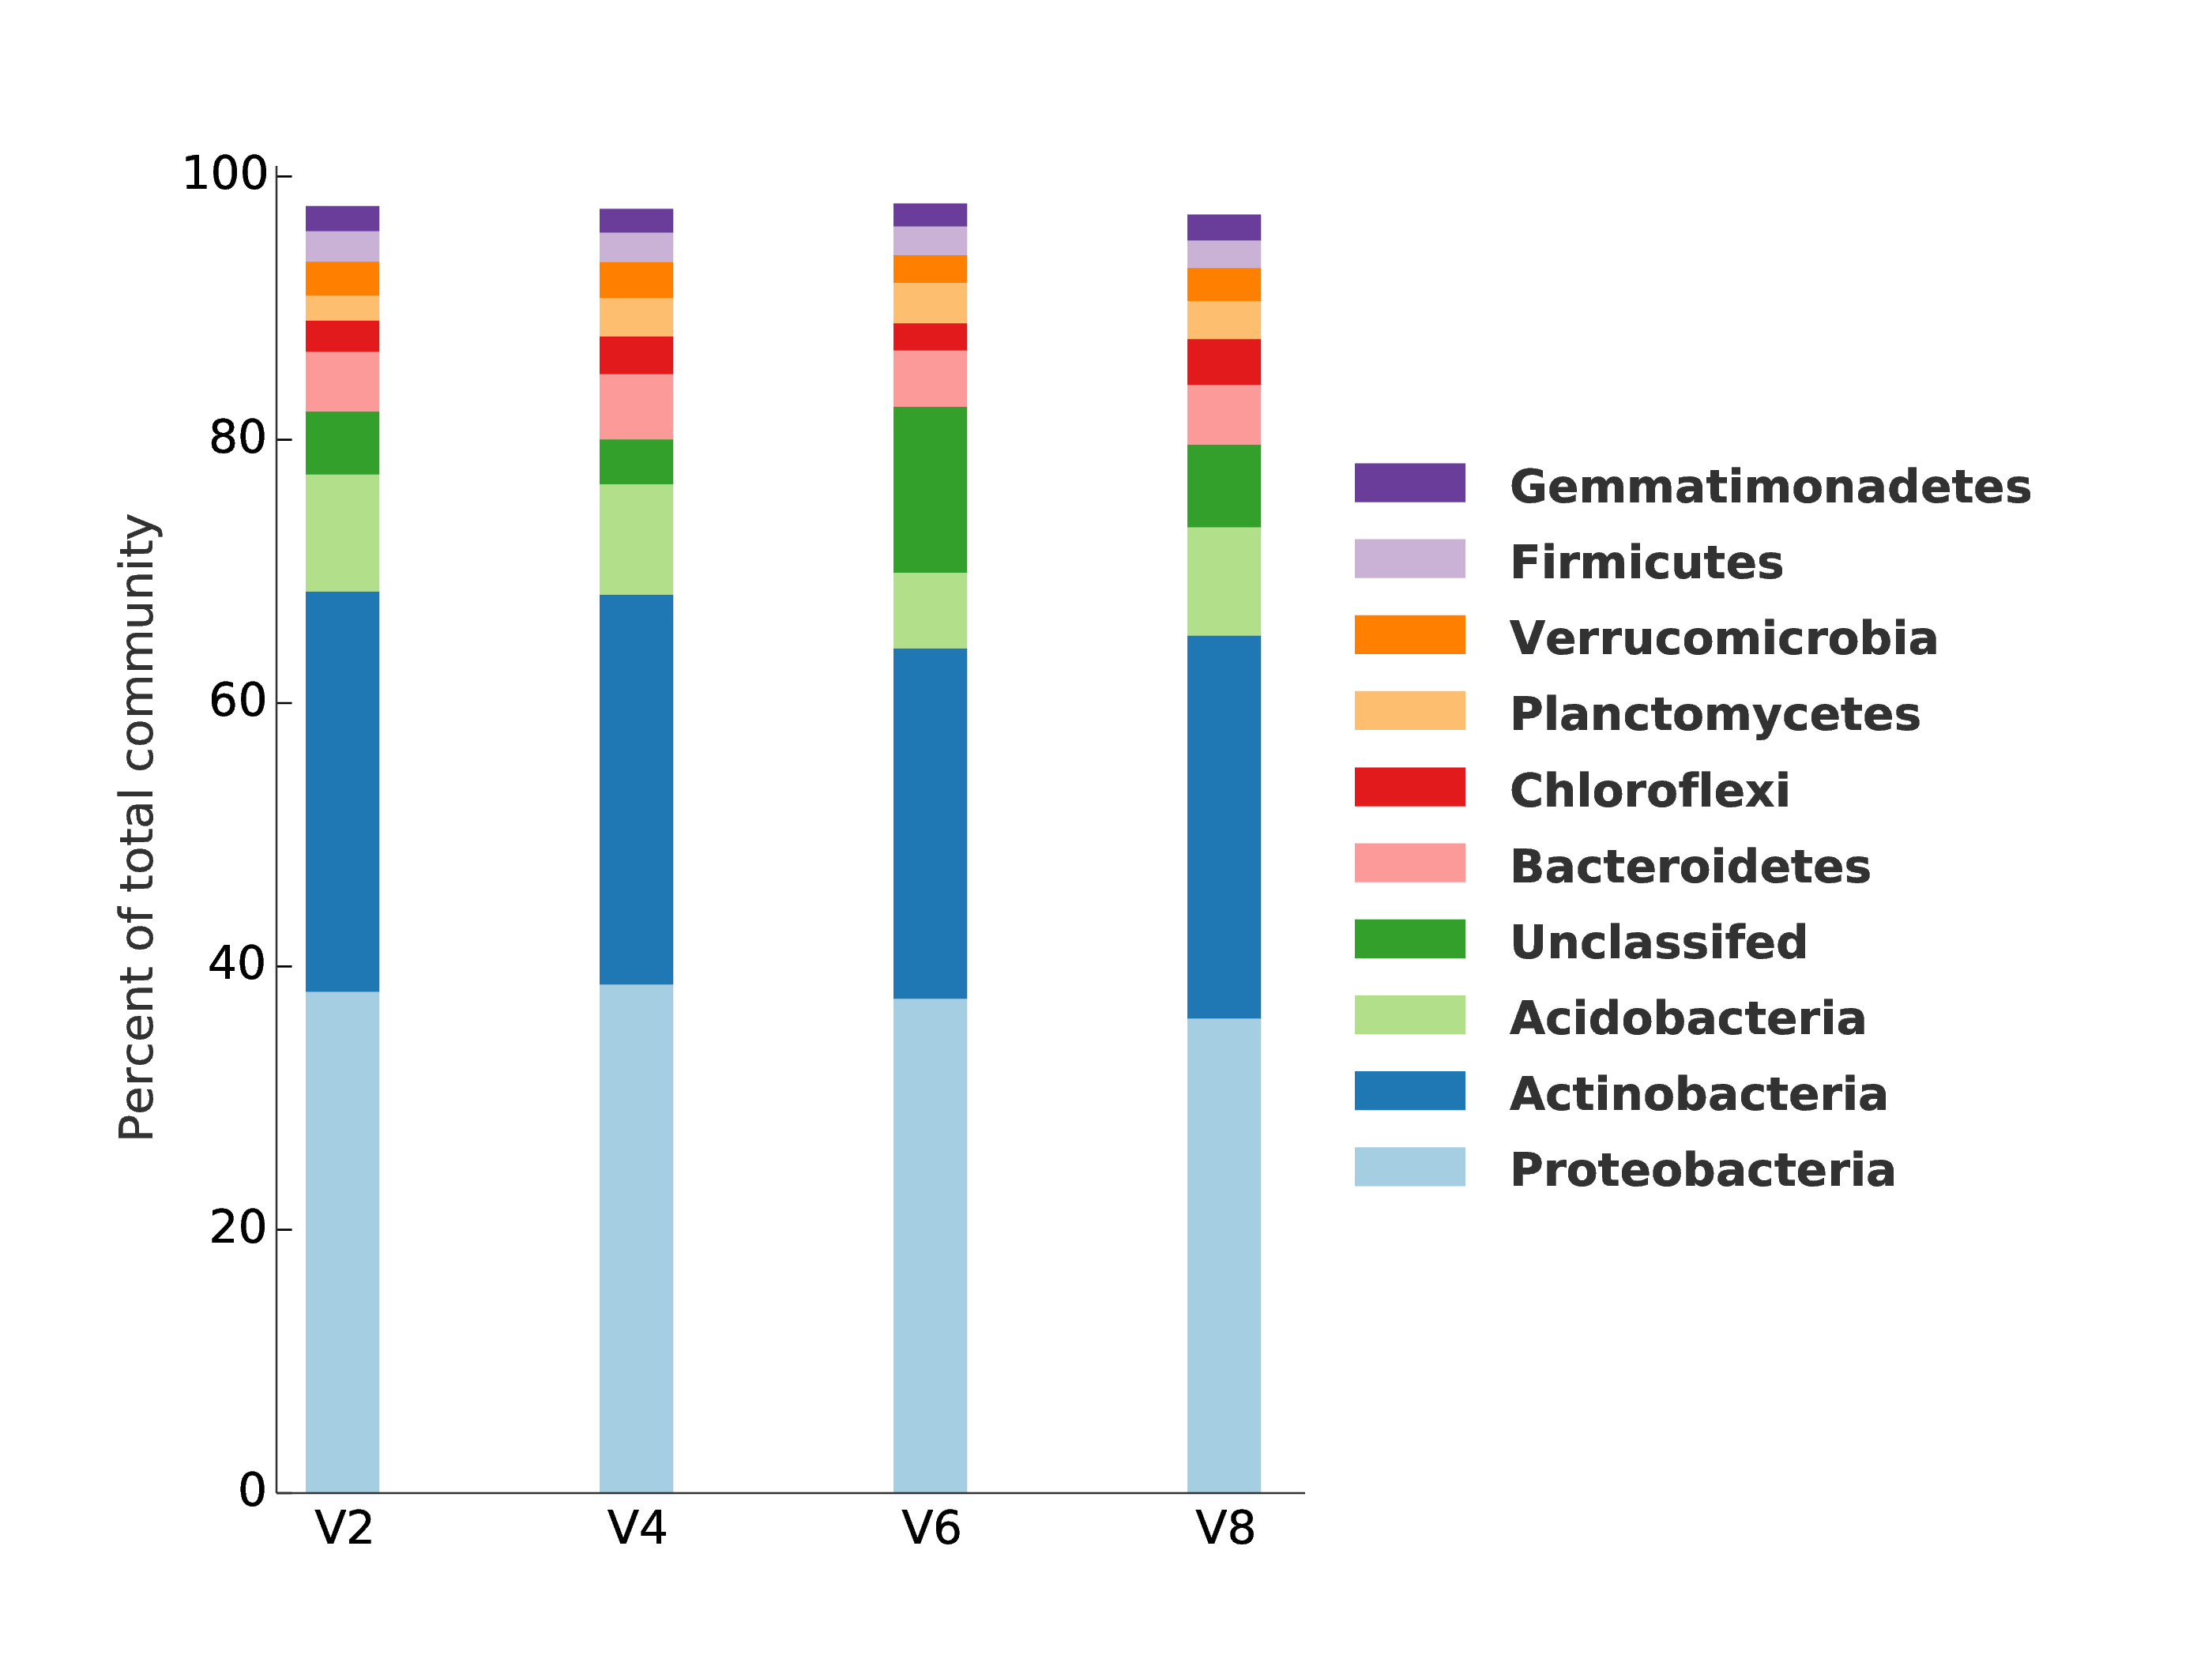
\includegraphics[width=0.80\textwidth]{figs/chap2_figS6}
  \caption[Bacterial phylum profile comparison using different variable regions]{Bacterial phylum profile comparison using different variable regions. Different variable regions have similar taxonomy profiles, except that V6 has more unclassified sequences. The minimum Pearson’s correlation between the regions is 0.96. Classifications were done using SSU rRNA gene fragments from Miscanthus rhizosphere soil sample (M1) and SILVA database as reference.}
  \label{fig:chap2FigS6}
\end{figure}


\begin{figure}[tbph!]
  \centering
  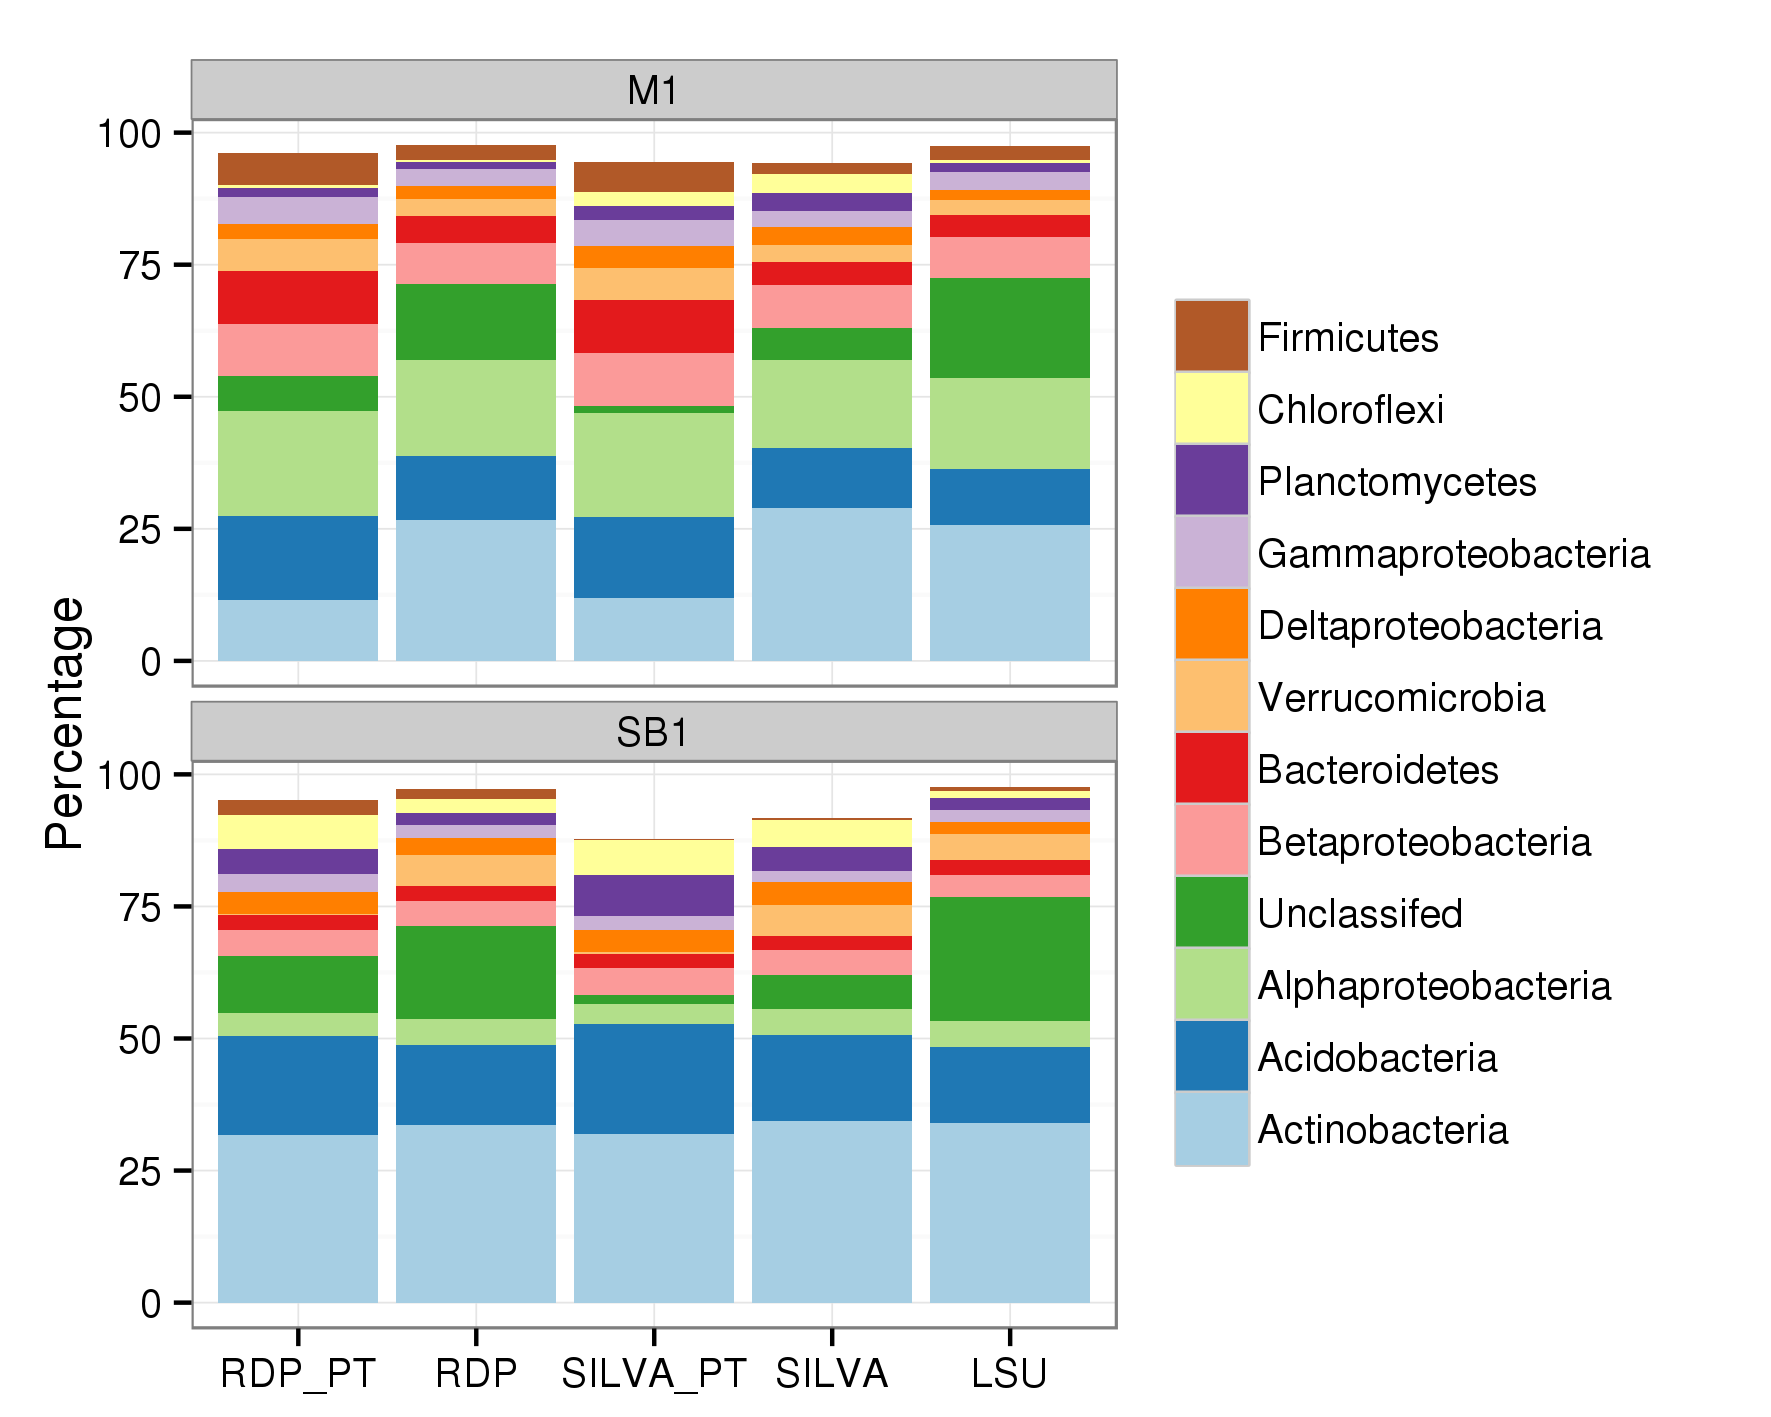
\includegraphics[scale=1]{figs/chap2_fig4}
  \caption[Phylum profiles of shotgun fragments from SSU and LSU rRNA genes and of amplicon reads]{Taxonomy profiles of Bacterial phyla of shotgun fragments from SSU and LSU rRNA genes and of amplicon reads. Classifications were done using both RDP and SILVA reference databases. ``\_PT'' indicates amplicon data. Lower panel is from bulk soil sample (SB1) and its amplicon data (\_PT) uses V6-V8 primer (515F/806R) and shows less Verrucomicrobia detected using both databases. Upper panel is rhizosphere sample (M1) and its amplicon data uses V4 primer (515F/806R) and shows less Actinobacteria and more Verrucomicrobia using both databases.}
  \label{fig:chap2Fig4}
\end{figure}


To take advantage of the fact that shotgun data is un-targeted, we retrieved and classified the Large Subunit (LSU) rRNA genes, which are co-transcribed with SSU rRNA genes. Their taxonomy profile was similar to that of SSU rRNA gene (Pearson’s correlation coefficient of 0.87 for SB1 and 0.91 for M1), except that more reads (19.6\%) remain unclassified (\cref{fig:chap2Fig4}). This is expected because of the much lower number of reference LSU rRNA genes in the SILVA database. The two genes show consistent community profiles at the Bacterial phylum level and also confirm the known primer bias against Verrrucomicrobia in 926F/1392R (V6-V8) primer set and also the bias against Actinobacteria in 515F/806R (V4) primer set (\cref{fig:chap2Fig4}). Further, both the LSU and SSU HMMs show the ability to identify Eukaryota members and give about the same taxonomy profile at domain level (\cref{fig:chap2FigS7}). It is noteworthy that both LSU and SSU shotgun data show Archaea to be twice as numerous (2\% vs. 1\%) in the bulk soil as the rhizosphere and that Eukaryota were much more numerous (6\% vs. 1\%) in the Miscanthus rhizosphere soil than the bulk soil (\cref{fig:chap2FigS7}). Higher fungal percentage (2.54\% vs. 0.39\%), fungi/bacteria ratio (0.027 vs. 0.004), and Arbuscular Mycorrhizal Fungi (AMF) percentage in fungi (0.18\% vs. 0) are found in rhizosphere sample (M1) than bulk soil sample (SB1) (Table \ref{tab:chap2TabS1}). Copy correction was applied on two soil samples (SB1 and M1). Both samples showed that Firmicutes and Bacteroidetes had the highest fold change after copy number correction (\cref{fig:chap2FigS8}). Despite copy number correction, the clustering of our soil samples did not change (\cref{fig:chap2FigS9}) compared to that without copy number correction (\cref{fig:chap2Fig1}), probably because of the low proportion of taxa with large rrn number corrections.


\begin{figure}[tbph!]
  \centering
  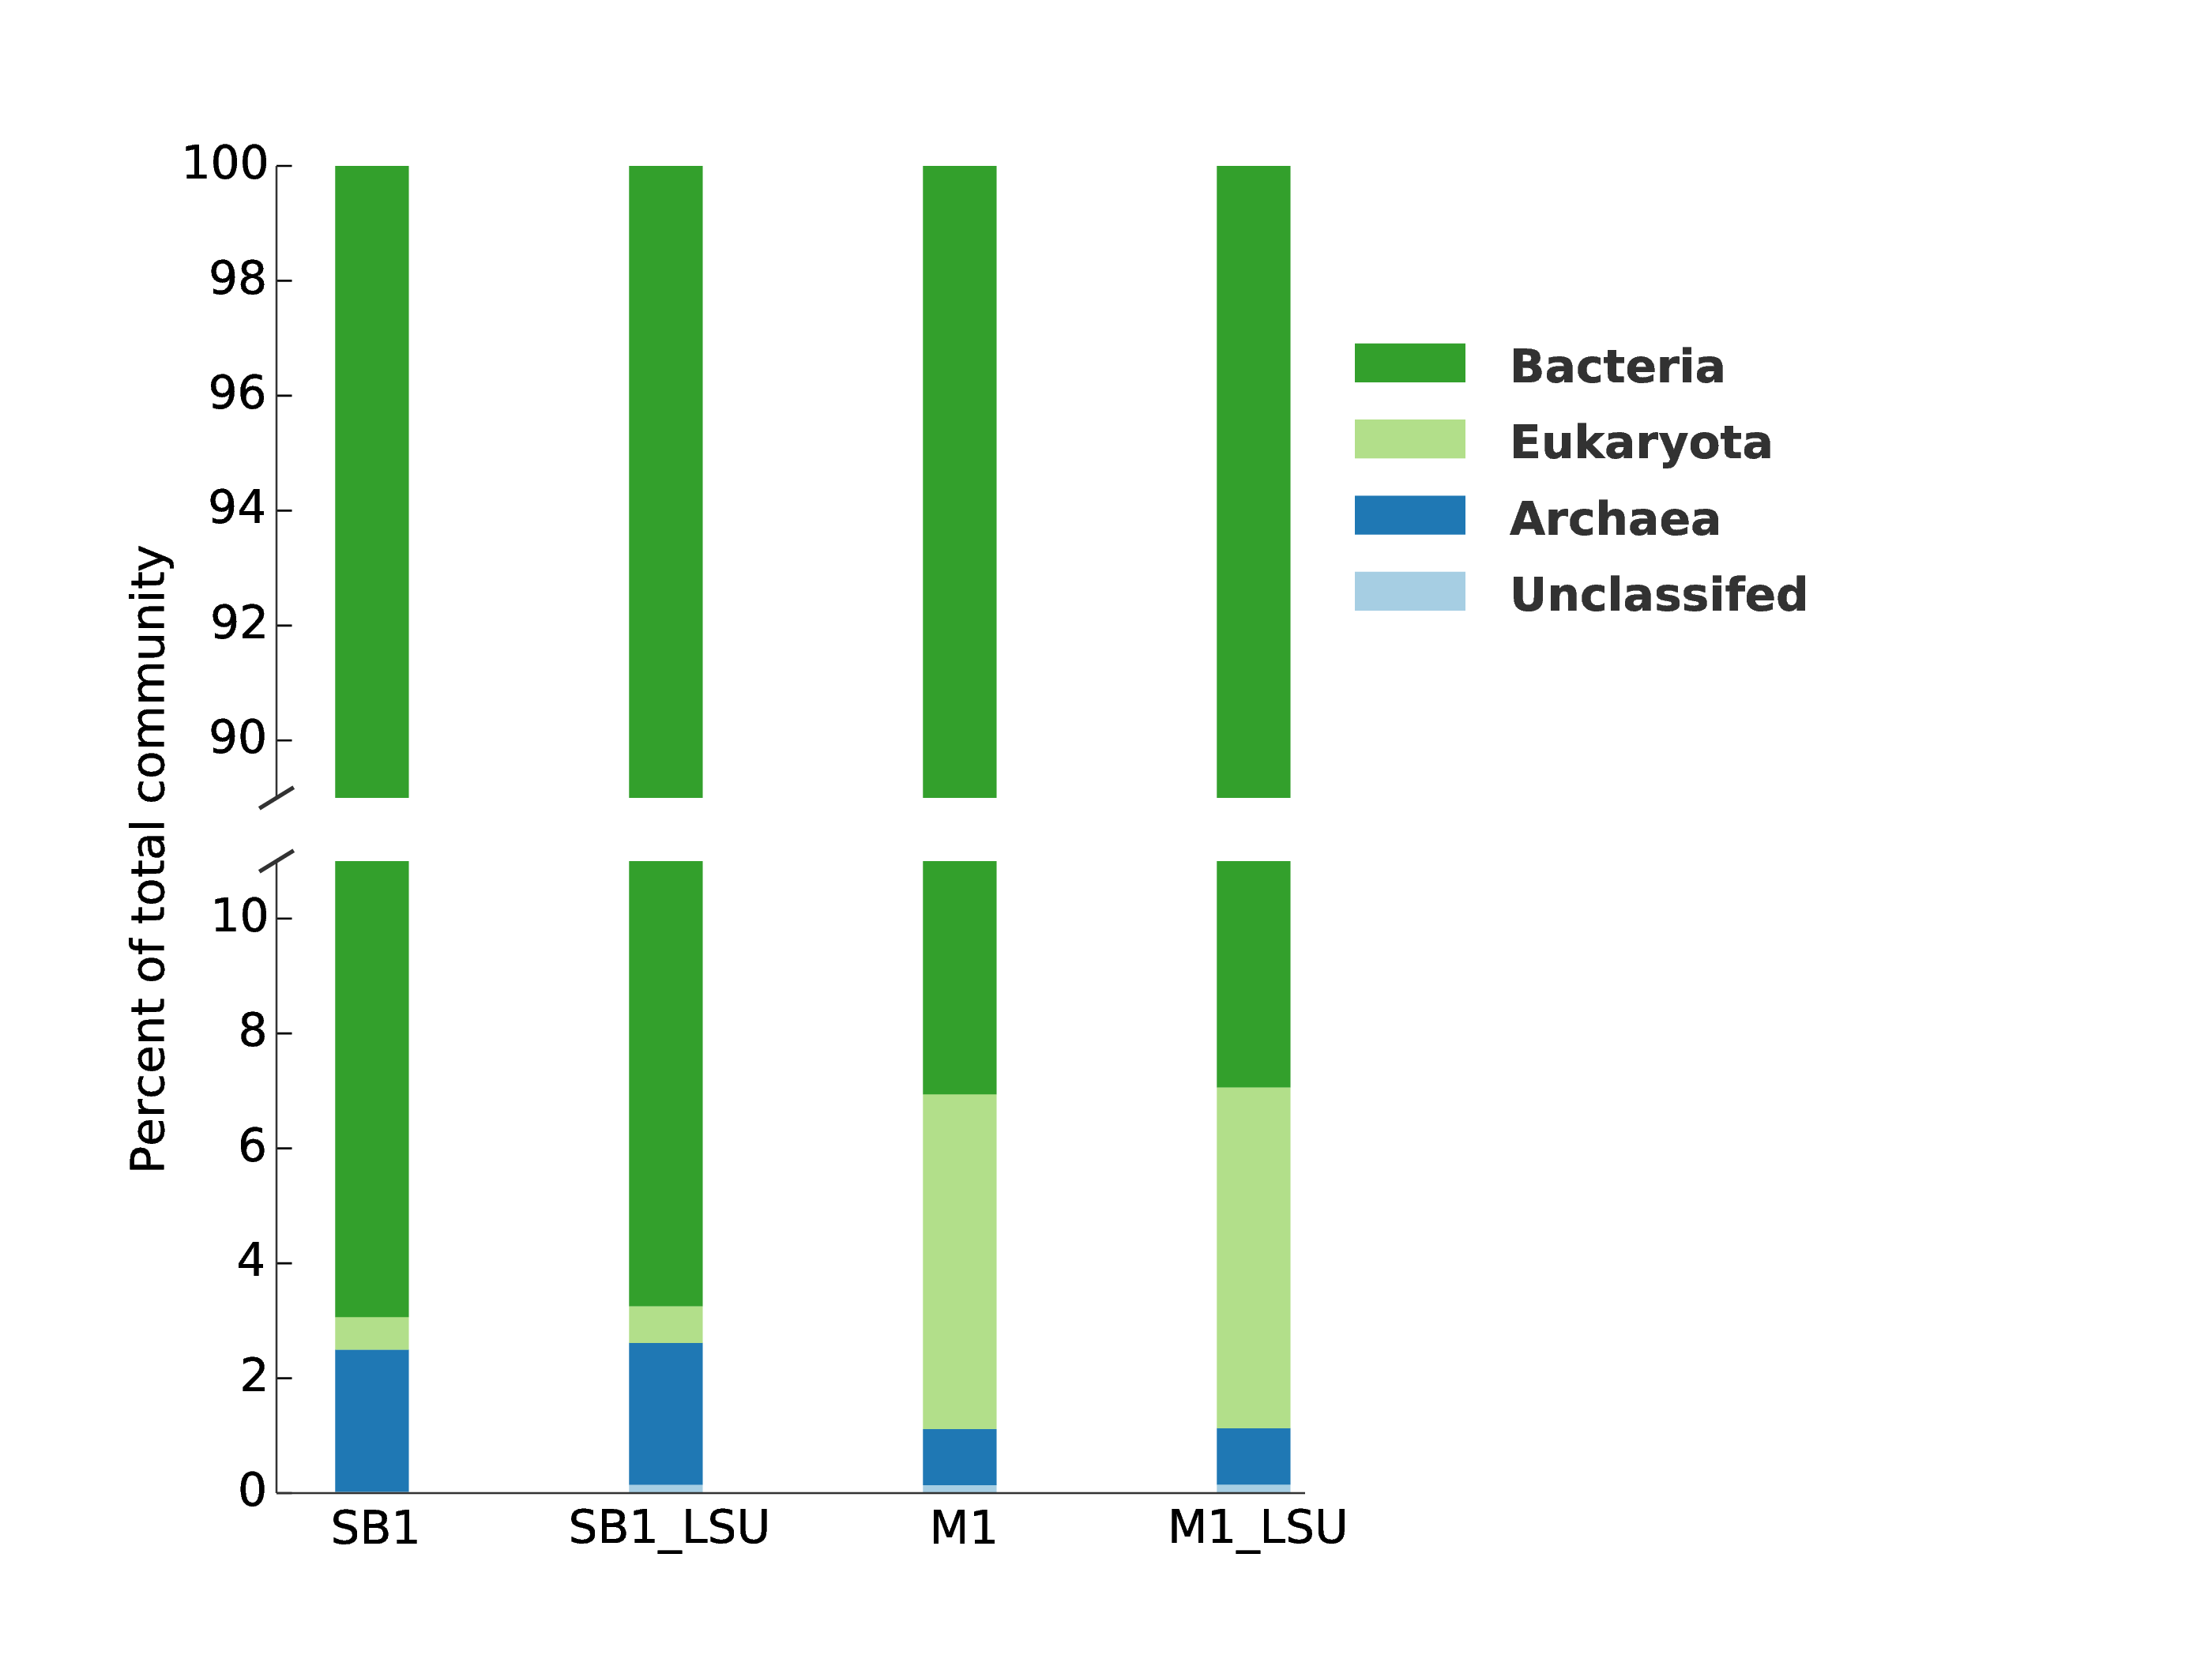
\includegraphics[width=0.80\textwidth]{figs/chap2_figS7}
  \caption[Taxonomy profile comparison at domain level using SSU and LSU rRNA genes]{Taxonomy profile comparison at domain level using SSU and LSU rRNA genes. For both the bulk soil sample (SB1) and rhizosphere sample (M1), SSU and LSU show consistent domain level taxonomy distribution (Pearson’s correlation coefficient = 1). ``\_LSU'' indicates taxonomy from LSU rRNA SILVA database and the rest are classified by SSU rRNA database.}
  \label{fig:chap2FigS7}
\end{figure}


\begin{table}[htbp]
  \centering
  \caption[Fungi/bacteria ratio and percent of AMF fungi in rhizosphere and bulk soil samples]{Higher fungi/bacteria ratio and percent of AMF fungi are in rhizosphere sample (M1) than bulk sample (SB1).}
    \begin{tabular}{|l|r|r|r|r|}
    \toprule
          & \multicolumn{1}{l|}{\% Bacteria} & \multicolumn{1}{l|}{\% Fungi} & \multicolumn{1}{l|}{\% AMF in Fungi} & \multicolumn{1}{l|}{Fungi/Bacteria} \\
    \midrule
    SB1-SSU & 97.00\% & 0.36\% & 0.00\% & 0.0037 \\
    \midrule
    SB1-LSU & 96.75\% & 0.42\% & 0.00\% & 0.0044 \\
    \midrule
    M1-SSU & 92.38\% & 2.60\% & 0.18\% & 0.0281 \\
    \midrule
    M1-LSU & 92.94\% & 2.48\% & 0.18\% & 0.0267 \\
    \bottomrule
    \end{tabular}%
  \label{tab:chap2TabS1}%
\end{table}%


\begin{figure}[tbph!]
  \centering
  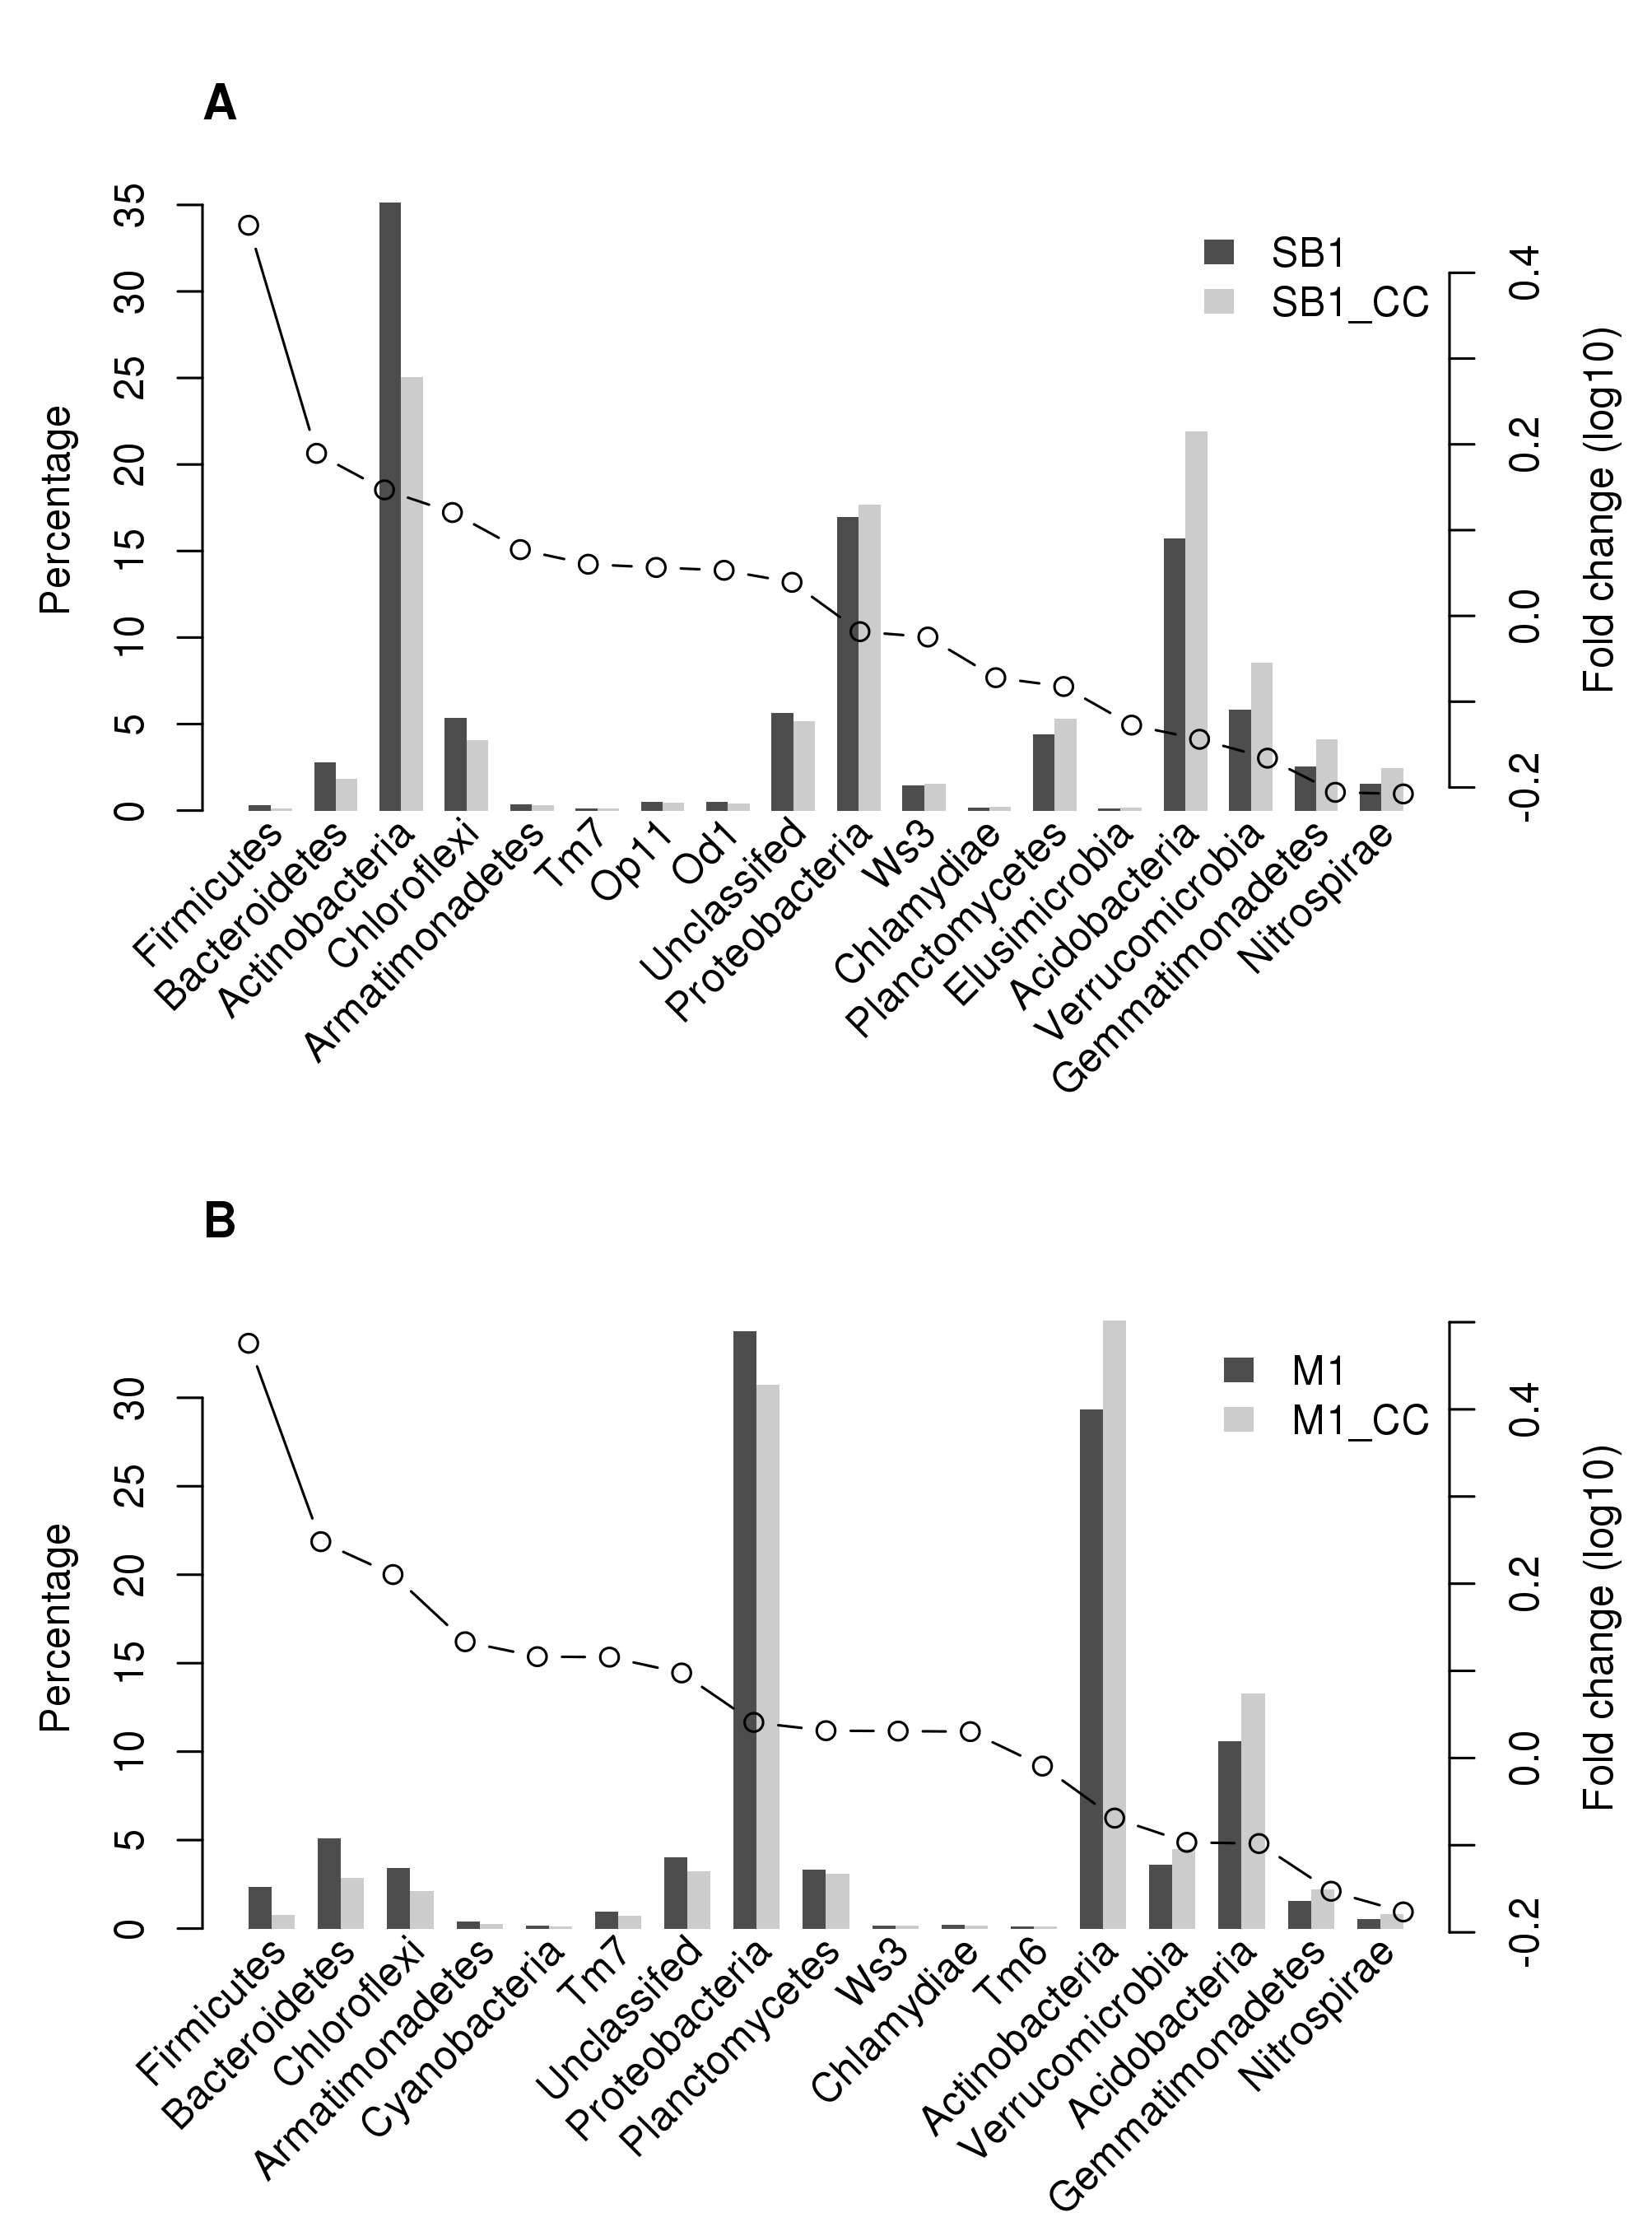
\includegraphics[width=0.80\textwidth]{figs/chap2_figS8}
  \caption[Bacterial phylum level taxonomy summary before and after SSU rRNA gene copy correction]{Bacterial phylum level taxonomy summary before and after SSU rRNA gene copy correction. Left vertical axis with bar plot shows percentage in total community, while right vertical axis with line plot shows fold change after copy number correction. Taxa with relative abundances of more than 0.1\% before copy correction were chosen and were ordered based on fold change. Subfigure A is for bulk soil sample (SB1) and B is for Miscanthus rhizosphere sample (M1).}
  \label{fig:chap2FigS8}
\end{figure}


\begin{figure}[tbph!]
  \centering
  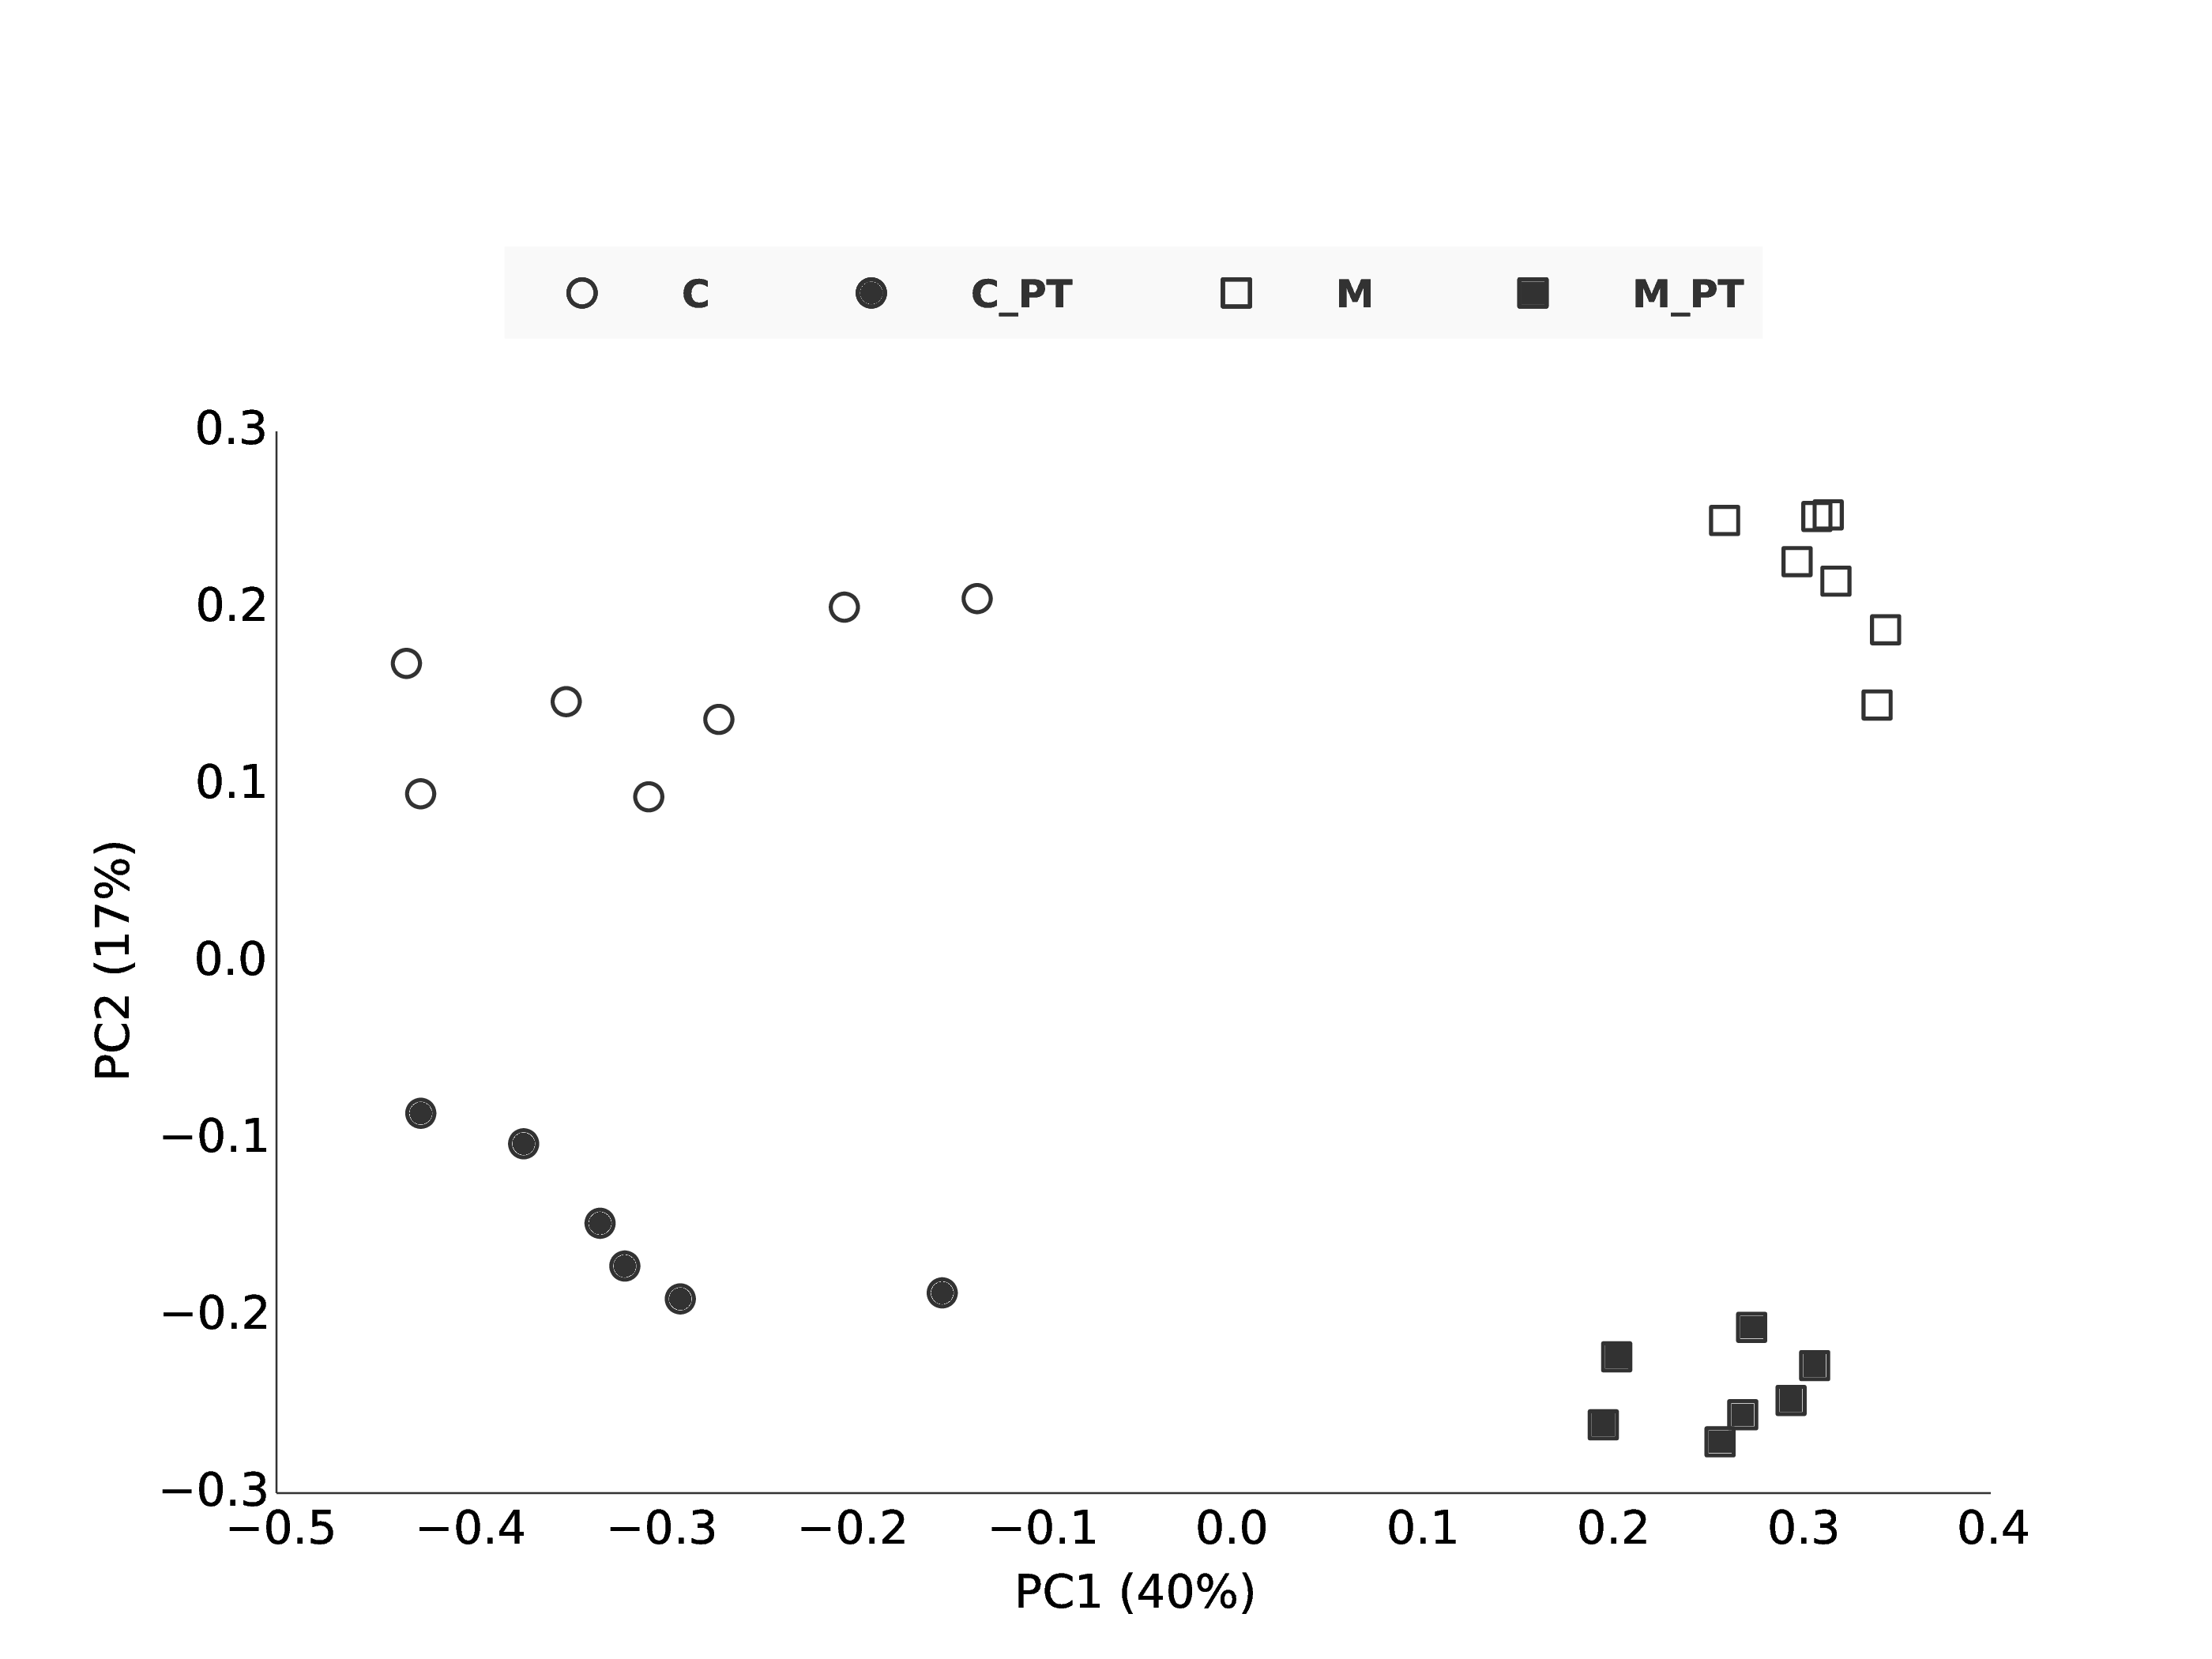
\includegraphics[width=0.80\textwidth]{figs/chap2_figS9}
  \caption[Ordination plot of amplicon and shotgun derived data after copy correction]{Ordination plot of amplicon and shotgun derived data after copy correction. The plot is similar to the one without copy correction (\cref{fig:chap2Fig3}). There were significant differences in amplicon and shotgun derived data (y-axis) and of corn and Miscanthus rhizosphere samples (x-axis), (AMOVA p-value < 0.001), after copy number correction. PCoA was applied to OTU table resulting from de novo clustering with shotgun data and amplicon data using 150bp of V4 region. The filled markers (``\_PT'') are amplicon data and the unfilled markers are shotgun data.}
  \label{fig:chap2FigS9}
\end{figure}


\section{Discussion}

We present, characterize and validate an efficient method for retrieving and analyzing SSU rRNA gene fragments from shotgun metagenomic sequences. The pipeline enables unsupervised diversity analysis with copy number correction on multiple variable regions, has the scalability to handle large soil metagenomes, is expandable to other phylogenetic marker genes and is publicly available on GitHub.

We apply a two-step approach for retrieving SSU rRNA gene fragments, a loose HMM filtering step followed by a more stringent step that screens by identity to the best match reference. The first step leverages HMMER \cite{eddy_new_2009} and should thus have better scalability than existing shotgun analysis pipelines that use BLAST-like tools such as MG-RAST \cite{sunagawa_metagenomic_2013}. MG-RAST annotates shotgun reads by BLAT search against rRNA databases and the taxonomy of reads is inferred from the best hit or least common ancestor of several top hits \cite{meyer_metagenomics_2008,altschul_gapped_1997,kent_blatblast-like_2002}. BLAT or BLAST-like tools are not scalable for large datasets and must be run in parallel on large computer clusters, because BLAST-like tools typically do pairwise comparison of reads against large and growing rRNA database such as RDP, SILVA and GreenGenes \cite{cole_ribosomal_2014,quast_silva_2013,desantis_greengenes_2006}, while HMM-based methods compare reads to only fixed number of models (commonly one for each domain) and thus more scalable \cite{sunagawa_metagenomic_2013}. Moreover, these pipelines lack unsupervised community analysis. HMM-based search has been used before as it is fast and sensitive for rrn retrieval \cite{huang_identification_2009,           lee_rrnaselector:_2011,bengtsson_metaxa:_2011,shah_comparing_2011} and current existing implementations such as meta-rna, RNASelector and metaxa are all wrappers around HMMER \cite{eddy_new_2009}. We chose meta-rna and metaxa for comparison, for the reason that RNASelector can only run in graphic interface that is not suitable for large datasets.

The second step evaluates hmmsearch results based on identity to their best-match reference and also prepares the alignment of SSU RNA gene fragments for clustering. Since there is no clear sequence identity threshold for SSU rRNA genes, the choice of identity cutoff is arbitrary (the default is 50\%). This is also common practice in amplicon analysis platforms where reads with low identity to reference sequences are discarded prior to clustering \cite{schloss_introducing_2009,kuczynski_using_2012}. For consistency in comparison, sequences in our amplicon datasets with less than 50\% identity to reference sequences are also discarded. An alignment of the SSU rRNA gene fragments is essential for the later unsupervised analyses. In comparison to methods that use only the 16S rRNA gene in E.coli as alignment template \cite{luo_soil_2014}, our method takes advantages of the rich phylogenetic diversity of SSU rRNA genes provided by the SILVA database. Increasing the number of reference sequences can improve the quality of alignment, but also linearly increases the memory required \cite{schloss_high-throughput_2009,caporaso_pynast:_2010}.

Our unsupervised analysis with shotgun data is a novel and important part of the pipeline. Our tests shows that regions as small as 50 bp could be applied to clustering. Thus short reads around 50 bp could be applied to this method as long as there are sufficient numbers of reads aligned to the target region (sequencing depth is a limiting factor; see below). This is consistent with pilot studies from 454 amplicon sequencing \cite{liu_short_2007,sogin_microbial_2006}. When sequencing depth is limited, there is flexibility to control the number of reads to include for clustering by adjusting the target region size and read length cutoff within certain limits (\cref{fig:chap2FigS2} B). The caveat of using very short or very large target regions is that the overlapping portion of reads will decrease and thus decrease the accuracy of clustering and the impact of sequencing error will increase; for example, an error in a 50 bp read can cause 2\% distance and we will accordingly need to set a larger distance cutoff for clustering. In addition, we can obtain longer sequences from overlapping paired ends as shown in our soil data (\cref{fig:chap2FigS10}). Thus reads from Illumina shotgun data (ranging from 75 to 250 bp) can be used for unsupervised analysis. Note that the flexibility on choice of variable region for analysis is another advantage of shotgun data (\cref{fig:chap2FigS2} C).


\begin{figure}[tbph!]
  \centering
  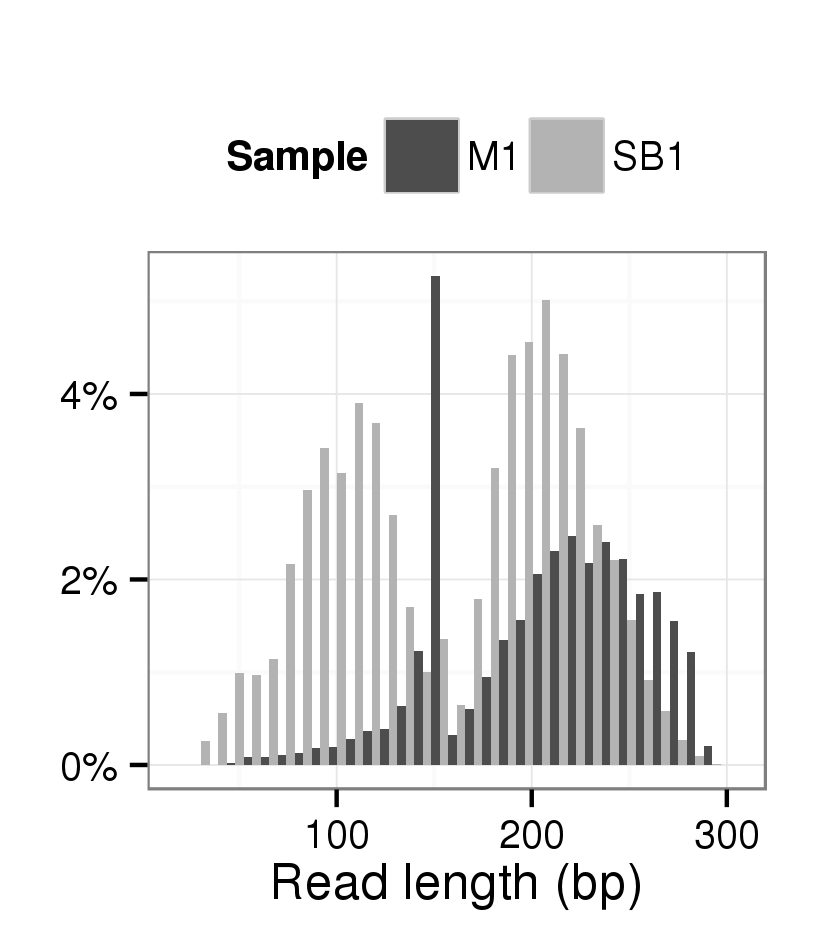
\includegraphics[scale=1]{figs/chap2_figS10}
  \caption[Length distribution of trimmed reads after quality trimming and paired-end merging]{Length distribution of trimmed reads after quality trimming and paired-end merging. SB1 is the bulk soil data and M1 is the rhizosphere data. The reads with >150 bp result from the merged paired ends, which benefits classification and clustering in downstream analyses. Reads less than 150 bp are also used in the analysis and come from unmerged paired reads.}
  \label{fig:chap2FigS10}
\end{figure}

We also found good reproducibility of OTU abundance between technical replicates, which is critical for the validity of our method (\cref{fig:chap2FigS4} A). Generally, OTU-based analysis provides higher resolution than taxonomy-based diversity analysis for community comparison, largely due to the databases lacking reference sequences from uncultured microbes \cite{schloss_assessing_2011}. The high correlation of OTU abundance in two technical replicates shows the reproducibility of the analysis of shotgun data, which is comparable to the reproducibility of amplicon data shown in another study in terms of Pearson’s correlation and R2 of linear regression \cite{lundberg_defining_2012}. Further, comparison of OTU abundances in shotgun data and amplicon data sequenced from the same DNA extraction also show that many OTUs have inconsistent abundances between the two types of data (\cref{fig:chap2FigS4} C and D), which agrees with the differences seen in the taxonomy-based comparison (\cref{fig:chap2Fig4}).

Community comparison by ordination methods such as PCoA and NMDS is one of the most common analyses in microbial ecology. To the best of our knowledge, the methods used in two studies \cite{luo_soil_2014,sharpton_phylotu:_2011} are the only existing tools that are designed to deal with clustering of SSU rRNA gene fragments from Illumina shotgun data. The former could result in poor alignment by using only the 16S rRNA gene in E. coli as the alignment template. The latter (PhylOTU) was applied to longer shotgun sequences from Sanger sequencing in their study. It does the OTU clustering of SSU rRNA gene fragments aligned together over the whole gene length, which can be problematic because fragments aligned to different regions do not overlap and thus the clustering results are not reliable, even though the reference sequences included in the clustering process can improve the results. Since our tests shows that as low as 50 bp hyper-variable region can be used for unsupervised analyses (\cref{fig:chap2FigS2} A and C), we make sure all the sequences overlap by picking one small region (150 bp) and all sequences included in clustering have lengths longer than 100 bp in our clustering method. In addition, longer reads obtained by assembling overlapping paired end reads (\cref{fig:chap2FigS10}) can make use of more overlap among reads and thus are more suitable for clustering. As read lengths increase with improvement of sequencing technology, longer regions can be chosen and the clustering results will be even more reliable. Also, shotgun data provides the flexibility to choose any variable region (\cref{fig:chap2Fig2,fig:chap2Fig3,fig:chap2FigS6,fig:chap2FigS2} C), and the consistency of results from different variable regions provides more confidence in the biological conclusion as well as the method itself.

Primer bias is a major limitation of amplicon methods, which was apparent in our comparisons of community profiles from amplicon versus shotgun data (\cref{fig:chap2Fig4}). Commonly, it is difficult to tell a bias is caused by primer or DNA extraction. The paired amplicon and shotgun data from the same DNA extract provides us a new opportunity to evaluate this issue, since the difference is only from the sequencing step. We used two main SSU rRNA gene databases, RDP and SILVA, to make sure the taxonomy distribution was not biased by the choice of reference databases and further confirmed by taxonomy distribution by the LSU rRNA gene. The bias against Verrucomicrobia with V6-V8 primers is consistent with other studies showing that Verrucomicrobia’s abundance in soil samples is underestimated due to primer bias \cite{bergmann_under-recognized_2011}. Meanwhile, the bias towards Verrucomicrobia with V4 primers agrees with studies showing that V4 primer set has better coverage of Verrucomicrobia \cite{bergmann_under-recognized_2011}. Furthermore, the V4 primer set shows bias against Actinobacteria. The V4 primer set is reported to cover 92.4\% of Actinobacteria in reference databases, the lowest among nine common bacterial phyla \cite{bergmann_under-recognized_2011}. Bias against Actinobacteria has also been reported in a study on synthetic community where no primer mismatch was found with members from Actinobacteria \cite{shakya_comparative_2013}, and another study on environmental samples using Sanger sequencing (24F/1492R) \cite{farris_detection_2007}, suggesting that in-silico evaluation of primers is not sufficient and some factors other than primer mismatch are causing the bias, for example, competition between primers and melting temperature \cite{parada_every_2015}. Thus primer bias detection by comparing paired amplicon and shotgun data is superior to methods that only search primers in the reference databases. 

Another advantage of our method over amplicon approaches is that we can identify the SSU rRNA gene from Bacteria, Archaea and Eukaryota. Fungi are of special interest in microbial ecology due their critical role in ecosystems \cite{lindahl_fungal_2013,porras-alfaro_genus_2014}. The Fungi/Bacteria ratio is an important indicator of C/N ratio and soil health \cite{de_vries_fungal/bacterial_2006,waring_differences_2013}. Our shotgun metagenome (DNA based) shows a ratio of 0.004 in bulk soil (SB1) and 0.027 in rhizosphere soil (M1) (Table \ref{tab:chap2TabS1}), while studies using Phospholipid Fatty-acid Analysis (PLFA) at the same sampling site (KBS) typically shows a ratio of 1 to 1.3 (58). The difference can be explained by higher biomass of fungi relative to DNA, since some fungi hyphae may not be filled with nuclei. In addition, we also found higher percentage of AMF (Abuscular Mycorrhiza Fungi) of rhizosphere soil (M1) compared to bulk soil (SB1), which is consistent with their symbiotic relationship with grass roots.

We also show that copy number correction can be achieved in our pipeline. Gene copy number is another source of bias that limits one’s ability to accurately profile microbial communities. There are up to 15 SSU rRNA gene copies in some Bacteria and up to 5 in Archaea \cite{acinas_divergence_2004}. This pipeline utilizes the SSU rRNA copy database in CopyRighter \cite{angly_copyrighter:_2014}. As expected, the Firmicutes in soil samples have the highest fold change (\cref{fig:chap2FigS8}). But, due to their low proportion in these soils, the impact of copy number correction on the overall community profile was minor (\cref{fig:chap2FigS9}). Copy number correction, however, is still an open problem because SSU rRNA gene copy number data for most species and/or OTUs are lacking and copy number can be incorrect even for species with complete genome sequences because of mis-assembly of these repeated regions. 

Sequencing depth is another important factor in considering this method for diversity analysis. The percentage of SSU rRNA gene fragments in shotgun data varies depending on the SSU rRNA gene copy number and genome size of each member. In our bulk soil sample (SB1) and the Miscanthus rhizosphere soil sample (M1), we classified about 0.03\% and 0.04\% of the total shotgun data as SSU rRNA, respectively. In an ideal situation we want to get enough SSU rRNA gene fragments to see saturation of rarefaction curve in OTU-based analysis, which is difficult for soil samples because of their high diversity and the presence of sequencing error. However, studies have shown that near saturation sequencing of SSU rRNA amplicons is not necessary for beta-diversity analysis \cite{caporaso_ultra-high-throughput_2012,kuczynski_microbial_2010}. Thus tmpirical fold coverage of 3000 based on the whole length (about 1500 bp) of SSU rRNA gene is suggested for surface soil samples, which requires 11.2 (1500*3000/0.04\%) Gbp of shotgun data, assuming the SSU rRNA gene comprises about 0.04\% of total data.

In this study, the LSU rRNA gene was used mainly as confirmation for SSU rRNA gene-based diversity analysis (\cref{fig:chap2Fig4,fig:chap2FigS7}). However, the LSU rRNA gene offers additional stretches of variable and characteristic sequence regions due to its longer sequence length, and thus yields better phylogenetic resolution \cite{hunt_evaluation_2006}. For the above reason and also the reason that there are more available references for fungi, the LSU rRNA gene is more commonly used for fungal community studies \cite{mummey_evaluation_2007,liu_accurate_2012,porter_factors_2012,begerow_current_2010}. Currently the use of the LSU rRNA gene is limited by reference sequences and universal primer sets available \cite{hunt_evaluation_2006}, but its increased resolution should not be overlooked since too limited resolution of the SSU rRNA gene is a barrier in many ecological studies \cite{lindahl_fungal_2013}. In the future, other single copy genes with phylogenetic reference and finer resolution, such as rplB, gyrB, and recA, could also be recovered from metagenomic sequence and used for community structure analysis by a similar pipeline \cite{roux_comparison_2011}.

\section{Conclusion}

We developed a fast and efficient pipeline that enables unsupervised diversity analysis with Illumina shotgun data. The pipeline has the scalability to analyze large datasets (5 CPU hours for 38 Gb data, with 4.8 Gb peak memory) and can be run on most desktops with more than 5 GB of memory. Since SSU rRNA based community analysis is an important method in microbial ecology, this method can save projects with existing shotgun sequence data from the additional cost of SSU rRNA amplicon sequencing. Moreover, shotgun sequencing are not as affected by primer bias and chimeras as amplicon sequencing and thus can improve the measurement of microbial community structure. As read length and sequencing depth increases, longer and more SSU rRNA gene fragments can be recovered. Thus clustering and diversity analysis by this pipeline will become even more reliable.


\chapter{Genomic and metagenomic comparison of \textit{rplB} and SSU rRNA gene species resolution}

\section{Introduction}

Microorganisms harness the majority of species and genetic diversity in biosphere shaped by 3.5 billion years of evolution \cite{locey_scaling_2016}. However, our understanding of microbial diversity is very limited mainly because the majority of them can not be cultured in lab conditions. Since late 1970s, SSU rRNA gene has made big progress in microbial species idenfication and is commonly used in microbial community diversity analysis \cite{woese_phylogenetic_1977,lane_rapid_1985,huse_exploring_2008,caporaso_ultra-high-throughput_2012}. But the facts that SSU rRNA gene is highly conserved and there could be multiple copies in the same genome and intra-genomic variation make SSU rRNA gene not effective in taxonomy identification at species and strain levels \cite{case_use_2007,roux_comparison_2011,wu_simple_2008}.

With fast accumulation of microbial genomes in NCBI in recent years \cite{land_insights_2015}, whole genome based comparison is considered to be the most accurate for species and strain identification \cite{goris_dna-dna_2007,luo_genome_2011,varghese_microbial_2015}. However, whole genome based comparison is computationally more expensive compared to marker genes and more importantly we are not able to get genome sequences of members in microbial community, especially for complex environments such as soil. Thus genome based definition does not work for community diversity analysis and marker genes are still essential for microbial community diversity analysis.

Due to disadvantages of SSU rRNA gene, microbial ecologiests have been looking for alternatives and single copy protein coding housekeeping genes stand out for the following reasons. First, they are single copy in the genome and thus allow more accurate species and strain identification and OTU clustering than SSU rRNA gene that is limited by intra-genomic heterogeneity. Second, their are ubiquitous almost across three domains of life. Third, protein coding genes evolve faster than rRNA genes not only because rRNA genes are more conserved due to their critical role in ribosome \cite{carter_functional_2000} but also higher mutation rate at the third position of codon in protein coding genes \cite{case_use_2007}.

Here, we use a single copy protein coding gene, \textit{rplB} (coding ribosomal large subunit protein L2) to showcase the potential of using single copy housekeeping genes as an phylogenetic marker for microbial community diversity analysis. Although there are similar studies either using on genomic data or metagenomic data \cite{case_use_2007,roux_comparison_2011}, we compare \textit{rplB} and SSU rRNA gene with all bacterial genomes and also large soil shotgun metagenomic data that are magnitudes larger than previous studies. In genomic data analyses, our novelty is that we evaluate difference in quantity (i.e. how different two taxons are in gene sequence) rather quality (i.e. two taxons are different in gene sequence). In metagenomic data analyses, our novelty is that we focus on effects of two different genes on \textit{de novo} OTU based analyses (common practice in microbial diversity analyses), while previous studies focus on taxonomy identification \cite{case_use_2007,roux_comparison_2011}. 

\section{Methods}

\textbf{Downloading bacterial genomes. }
Bacterial genome assembly information from NCBI 
(\url{ftp://ftp.ncbi.nlm.nih.gov/genomes/refseq/bacteria/assembly\_summary.txt})
was used to construct the url to download each genome based on instruction described this link (\url{http://www.ncbi.nlm.nih.gov/genome/doc/ftpfaq/\#allcomplete}). Command line ``wget'' was used to retrieve the genome sequences with urls from the above step.

\textbf{SSU rRNA gene and \textit{rplB} extraction and pairwise comparison. }
SSU rRNA gene HMM (Hidden Mokov Model) from SSUsearch was used \cite{guo_microbial_2015}. Aligned nucleotide sequences of \textit{rplB} training set in RDP FunGene database were used to build HMM using hmmbuild command in HMMER (version 3.1b2) \cite{eddy_new_2009}. Then nhmmer command in HMMER was used to extract SSU rRNA gene and \textit{rplB} from all Bacterial genomes using score cutoff (-T) of 60. Next, nhmmer hits with more than 90\% of the model length were treated as target gene. For the purpose of comparing SSU rRNA gene distance and \textit{rplB} gene distance, only one copy of SSU rRNA gene is randomly picked for each genome. Pairwise comparison among gene sequences were done by vsearch (version 1.1.3) with ``--allpairs\_global --acceptall''. Then three species of interest including \textit{\textit{Rhizobium} leguminosarum}, \textit{Pseudomonas putida} and \textit{Escherichia coli} were chosen for closer examination of \textit{rplB} pairwise distances and SSU rRNA gene distances.

\textbf{Rhizosphere soil metagenomic data download and preprocess. }
Shotgun sequencing data were downloaded from JGI portal (\url{http://genome.jgi.doe.gov/}). JGI Project IDs for the 21 samples are listed in Table \ref{tab:S1}. The samples are from rhizosphere of three biofuel crops: corn (C), switchgrass (S) and Miscanthus (M). There are seven replicates for each crop.
Raw reads were quality trimmed by fastq-mcf (verison 1.04.662) (\url{http://code.google.com/p/ea-utils}) ``-l 50 -q 30 -w 4 -k 0 -x 0 --max-ns 0 -X'' and then overlapping paired-end reads were merged by FLASH (version 1.2.7) \cite{magoc_flash:_2011} with ``-m 10 -M 120 -x 0.20 -r 140 -f 250 -s 25 -t 1'', which has also been described in \cite{guo_microbial_2015}. 


% Table generated by Excel2LaTeX from sheet 'S1'
\begin{table}[htbp]
  \centering
  \caption[Rhizosphere soil shotgun metagenomic data]{Rhizosphere soil shotgun metagenomic data. }
    \begin{tabular}{|lrr|}
    \toprule
    Sample & \multicolumn{1}{l}{JGI project ID} & \multicolumn{1}{l|}{Data size (Gb)} \\
    \midrule
    C1    & 1023764 & 46 \\
    C2    & 1023767 & 39 \\
    C3    & 1023770 & 57 \\
    C4    & 1023773 & 53 \\
    C5    & 1023776 & 57 \\
    C6    & 1023779 & 51 \\
    C7    & 1023782 & 46 \\
    M1    & 1023785 & 56 \\
    M2    & 1023788 & 57 \\
    M3    & 1023791 & 50 \\
    M4    & 1023794 & 42 \\
    M5    & 1023797 & 45 \\
    M6    & 1023800 & 43 \\
    M7    & \multicolumn{1}{l}{1018623, 1018611} & 32 \\
    S1    & 1023803 & 40 \\
    S2    & \multicolumn{1}{l}{1018626, 1018614} & 28 \\
    S3    & 1023806 & 44 \\
    S4    & 1023809 & 49 \\
    S5    & \multicolumn{1}{l}{1018629, 1018617} & 27 \\
    S6    & 1023812 & 50 \\
    S7    & 1023815 & 39 \\
    \bottomrule
    \end{tabular}%
  \label{tab:S1}%
\end{table}%



\textbf{SSU rRNA gene and \textit{rplB} identification and comparison in soil metagenomes. }
SSU rRNA gene fragments and those aligned to V4 region (\textit{E. coli} position: 577 - 727) of each sample were identified using SSUsearch pipeline \cite{guo_microbial_2015} and then clustered by RDP McClust tool \cite{cole_ribosomal_2014}. In order to evaluate the effect of the two genes on OTUs number, it would be more fair to have both genes in full length rather than have \textit{rplB} in full length but SSU rRNA gene in partial length (V4). Thus emirge\_amplicon.py in EMIRGE (version 0.60.3) \cite{miller_short-read_2013} was used to assembly full length SSU rRNA genes using raw reads identified as SSU rRNA gene from corn samples by SSUsearch with ``-l 150 --phred 33 -a 4 -i 275 -s 25''.

Then full length \textit{rplB} sequences were assembled by Xander with flags 
``MAX\_JVM\_HEAP=500G, FILTER\_SIZE=40, K\_SIZE=45, genes=\textit{rplB}, THREADS=9''. 
Due to memory limit, data for each crop were assembled separately. Then assembled \textit{rplB} sequences (nucleotide and protein) from three crops were pooled and clustered by RDP McClust tool \cite{cole_ribosomal_2014}. An OTU table with OTU counts for each sample was made based on mean kmer coverage of the representative sequence of each OTU. 

Further, diversity analyses was done by vegan package in R (``rda'' for ordination and ``diversity'' for Shannon diversity index using OTU (count) table from clustering. For comparising the resolution of two genes in metagenomes, since SSU rRNA gene had higher sampling depth than \textit{rplB} due to multiple copy nature of SSU rRNA gene, even subsampling was needed. Thus unique full length sequences of both genes were re-inflated based the abundance information before even subsampling. The abundance information of \textit{rplB} sequences was in a file with the name ``*\_coverage.txt'' in \textit{rplB}/cluster directory from Xander. Meanwhile, the relative abundance information of SSU rRNA gene assemblies can be found the description field of assembled sequence file in fasta format as described in README.txt (NormPrior) in EMIRGE package. With the total coverage of the gene estimated from the reads identified as SSU rRNA gene (total\_bp / 1500), the abundance of each gene was estimated by multiplying relative abundance and total coverage of SSU rRNA gene.

\section{Results}

\textbf{SSU rRNA gene and \textit{rplB} copy number and intra-genome SSU identity. }
A total of 53865 Bacterial genomes were downloaded and 4457 of them were complete genomes. The maximum, mean and minimum of SSU rRNA gene copy number detected was 20, 2, and 1 among all genomes, while 16, 4 and 1 among complete genomes (Table \ref{tab:S2}). Multiple copies of \textit{rplB} within the same genome were also detected (Table \ref{tab:S2}), with a maximum of 6 among all genomes and 2 among complete genomes. In order to compare these two genes, they need to be both present in genomes. We found 46600 genomes and 4440 completed genomes with both genes. When looking at intra genome varition in completed genomes of \textit{R. leguminosarum}, \textit{P. putida} and \textit{E. coli}, we found \textit{E. coli} has largest varition among the three, with a minimum of 95.4\% (\cref{fig:intraGenome3species}).


% Table generated by Excel2LaTeX from sheet 'S2'
\begin{table}[htbp]
  \centering
  \caption[Summary of SSU rRNA gene and \textit{rplB} copy number in genomes]{Summary of SSU rRNA gene and \textit{rplB} copy number in genomes. }
    \begin{tabular}{|rrrrr|}
    \toprule
    \multicolumn{1}{|l}{Copy} & \multicolumn{1}{l}{SSU\_all} & \multicolumn{1}{l}{\textit{rplB}\_all} & \multicolumn{1}{l}{SSU\_complete} & \multicolumn{1}{l|}{\textit{rplB}\_complete} \\
    \midrule
    1     & 32576 & 635   & 53289 & 4443 \\
    2     & 3136  & 711   & 90    & 4 \\
    3     & 2649  & 560   & 14    & NA \\
    4     & 2264  & 585   & 3     & NA \\
    5     & 2006  & 372   & NA    & NA \\
    6     & 1603  & 484   & 1     & NA \\
    7     & 1333  & 556   & NA    & NA \\
    8     & 525   & 194   & NA    & NA \\
    9     & 222   & 92    & NA    & NA \\
    10    & 187   & 107   & NA    & NA \\
    11    & 114   & 58    & NA    & NA \\
    12    & 72    & 27    & NA    & NA \\
    13    & 58    & 26    & NA    & NA \\
    14    & 48    & 38    & NA    & NA \\
    15    & 8     & 4     & NA    & NA \\
    16    & 7     & 1     & NA    & NA \\
    18    & 1     & NA    & NA    & NA \\
    20    & 1     & NA    & NA    & NA \\
    \bottomrule
    \end{tabular}%
  \label{tab:S2}%
\end{table}%


\begin{figure}[tbph!]
  \centering
  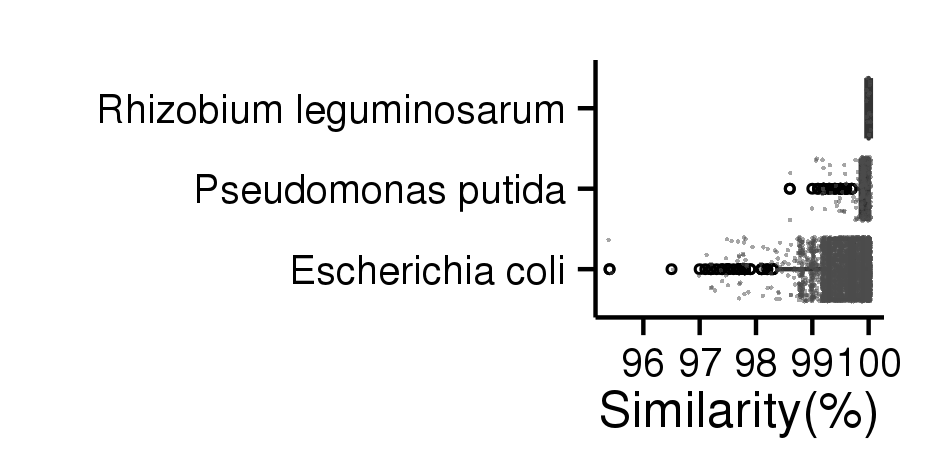
\includegraphics[scale=1]{figs/intra_genome_3species}

  \caption[Intra-genome varition of SSU rRNA gene]{Intra-genome varition of SSU rRNA gene of three species. \textit{E. coli} has largest varition among the three.}

  \label{fig:intraGenome3species}
\end{figure}

\textbf{Pairwise comparison of genomes with SSU rRNA gene and \textit{rplB}. }
Overall, \textit{rplB} gene distances were larger than SSU rRNA gene distances for most genome pairs \cref{fig:interSpeciesComp}. SSU rRNA gene distances were mainly between 90\% and 100\%, while \textit{rplB} distances were in a larger range between 70\% and 100\%. Further, we targeted several species of interest for detailed examination: \textit{R. leguminosarum}, \textit{P. putida} and \textit{E. coli} and found all selected species except \textit{E. coli} showed \textit{rplB} gene distances were larger than SSU rRNA gene within their corresponding family, genus, and species (among strains) (\cref{fig:RLeg,fig:PPutida,fig:EColi}). In contrast, most comparsion within genus and species for \textit{E. coli} showed SSU rRNA gene had larger distances than \textit{rplB}. SSU rRNA gene distances were mostly 99\% and \textit{rplB} distances were mostly 100\% (\cref{fig:EColi} B and C). The above results were from complete genomes. We also applied the same analyses with all genomes but some trains within the \textit{E. coli} showed too small identities (< 80 \% in identity) (\cref{fig:EColiAll}), indicating poor genome quality. Thus we decided to use results from completed genomes only. 


\begin{figure}[tbph!]
  \centering
  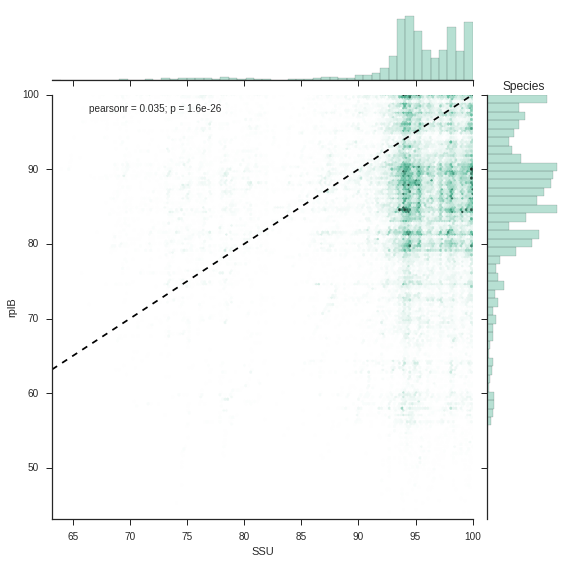
\includegraphics[width=0.80\textwidth]{figs/inter_species_comp}
  \caption[Pairwise comparison among genomes in the same genus using SSU rRNA gene and \textit{rplB}]{Pairwise comparison among genomes of species in the same genus using SSU rRNA gene and \textit{rplB}. SSU rRNA gene identities are larger than \textit{rplB} in most genomes. X axis is SSU rRNA gene identities and Y axis is \textit{rplB} identities. The dashed line is y = x.}
  \label{fig:interSpeciesComp}
\end{figure}


\begin{figure}[tbph!]
  \centering
  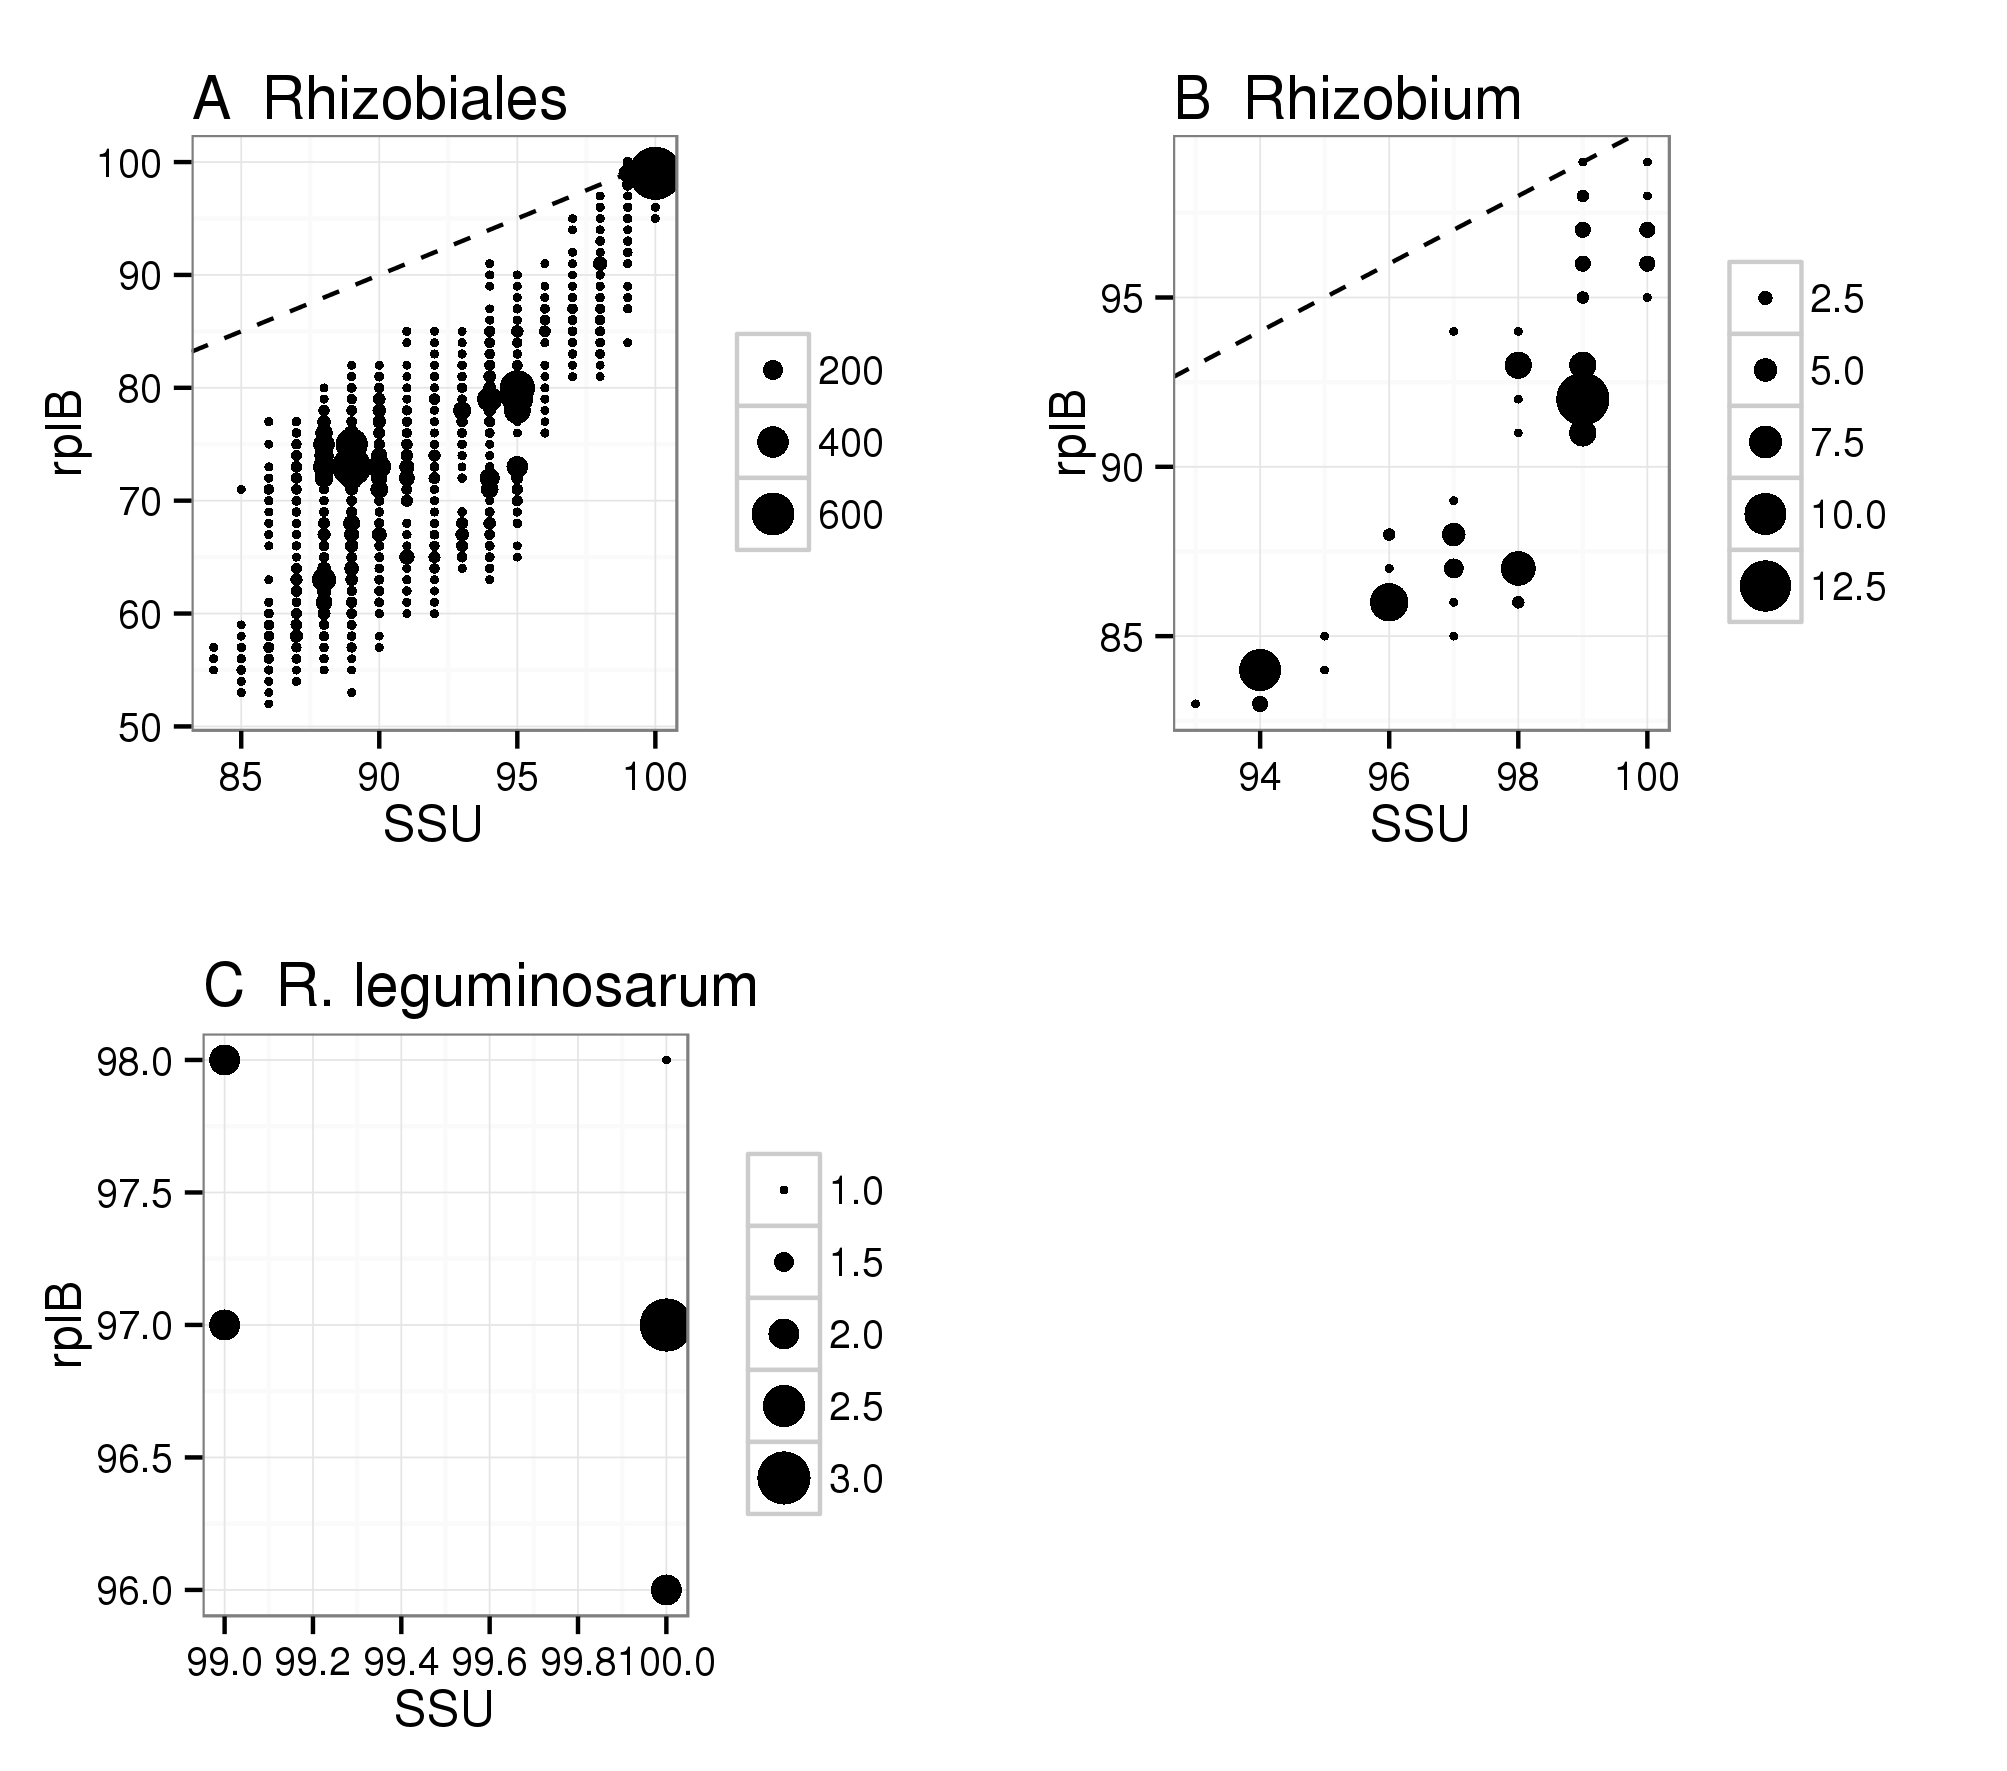
\includegraphics[scale=1]{figs/R_leg}
  \caption[Pairwise comparison among \textit{R. leguminosarum} genomes using SSU rRNA gene and \textit{rplB}]{Pairwise comparison among \textit{R. leguminosarum} genomes using SSU rRNA gene and \textit{rplB}. SSU rRNA gene identities are larger than \textit{rplB} in most genome pairs. X axis is SSU rRNA gene identities and Y axis is \textit{rplB} identities. The dashed line is y = x. A. All completed genomes in Rhizobiales are included in pairwise comparison; B. All completed genomes in \textit{\textit{Rhizobium}} are included; C. All completed genomes in \textit{R. leguminosarum} are included.}
  \label{fig:RLeg}
\end{figure}


\begin{figure}[tbph!]
  \centering
  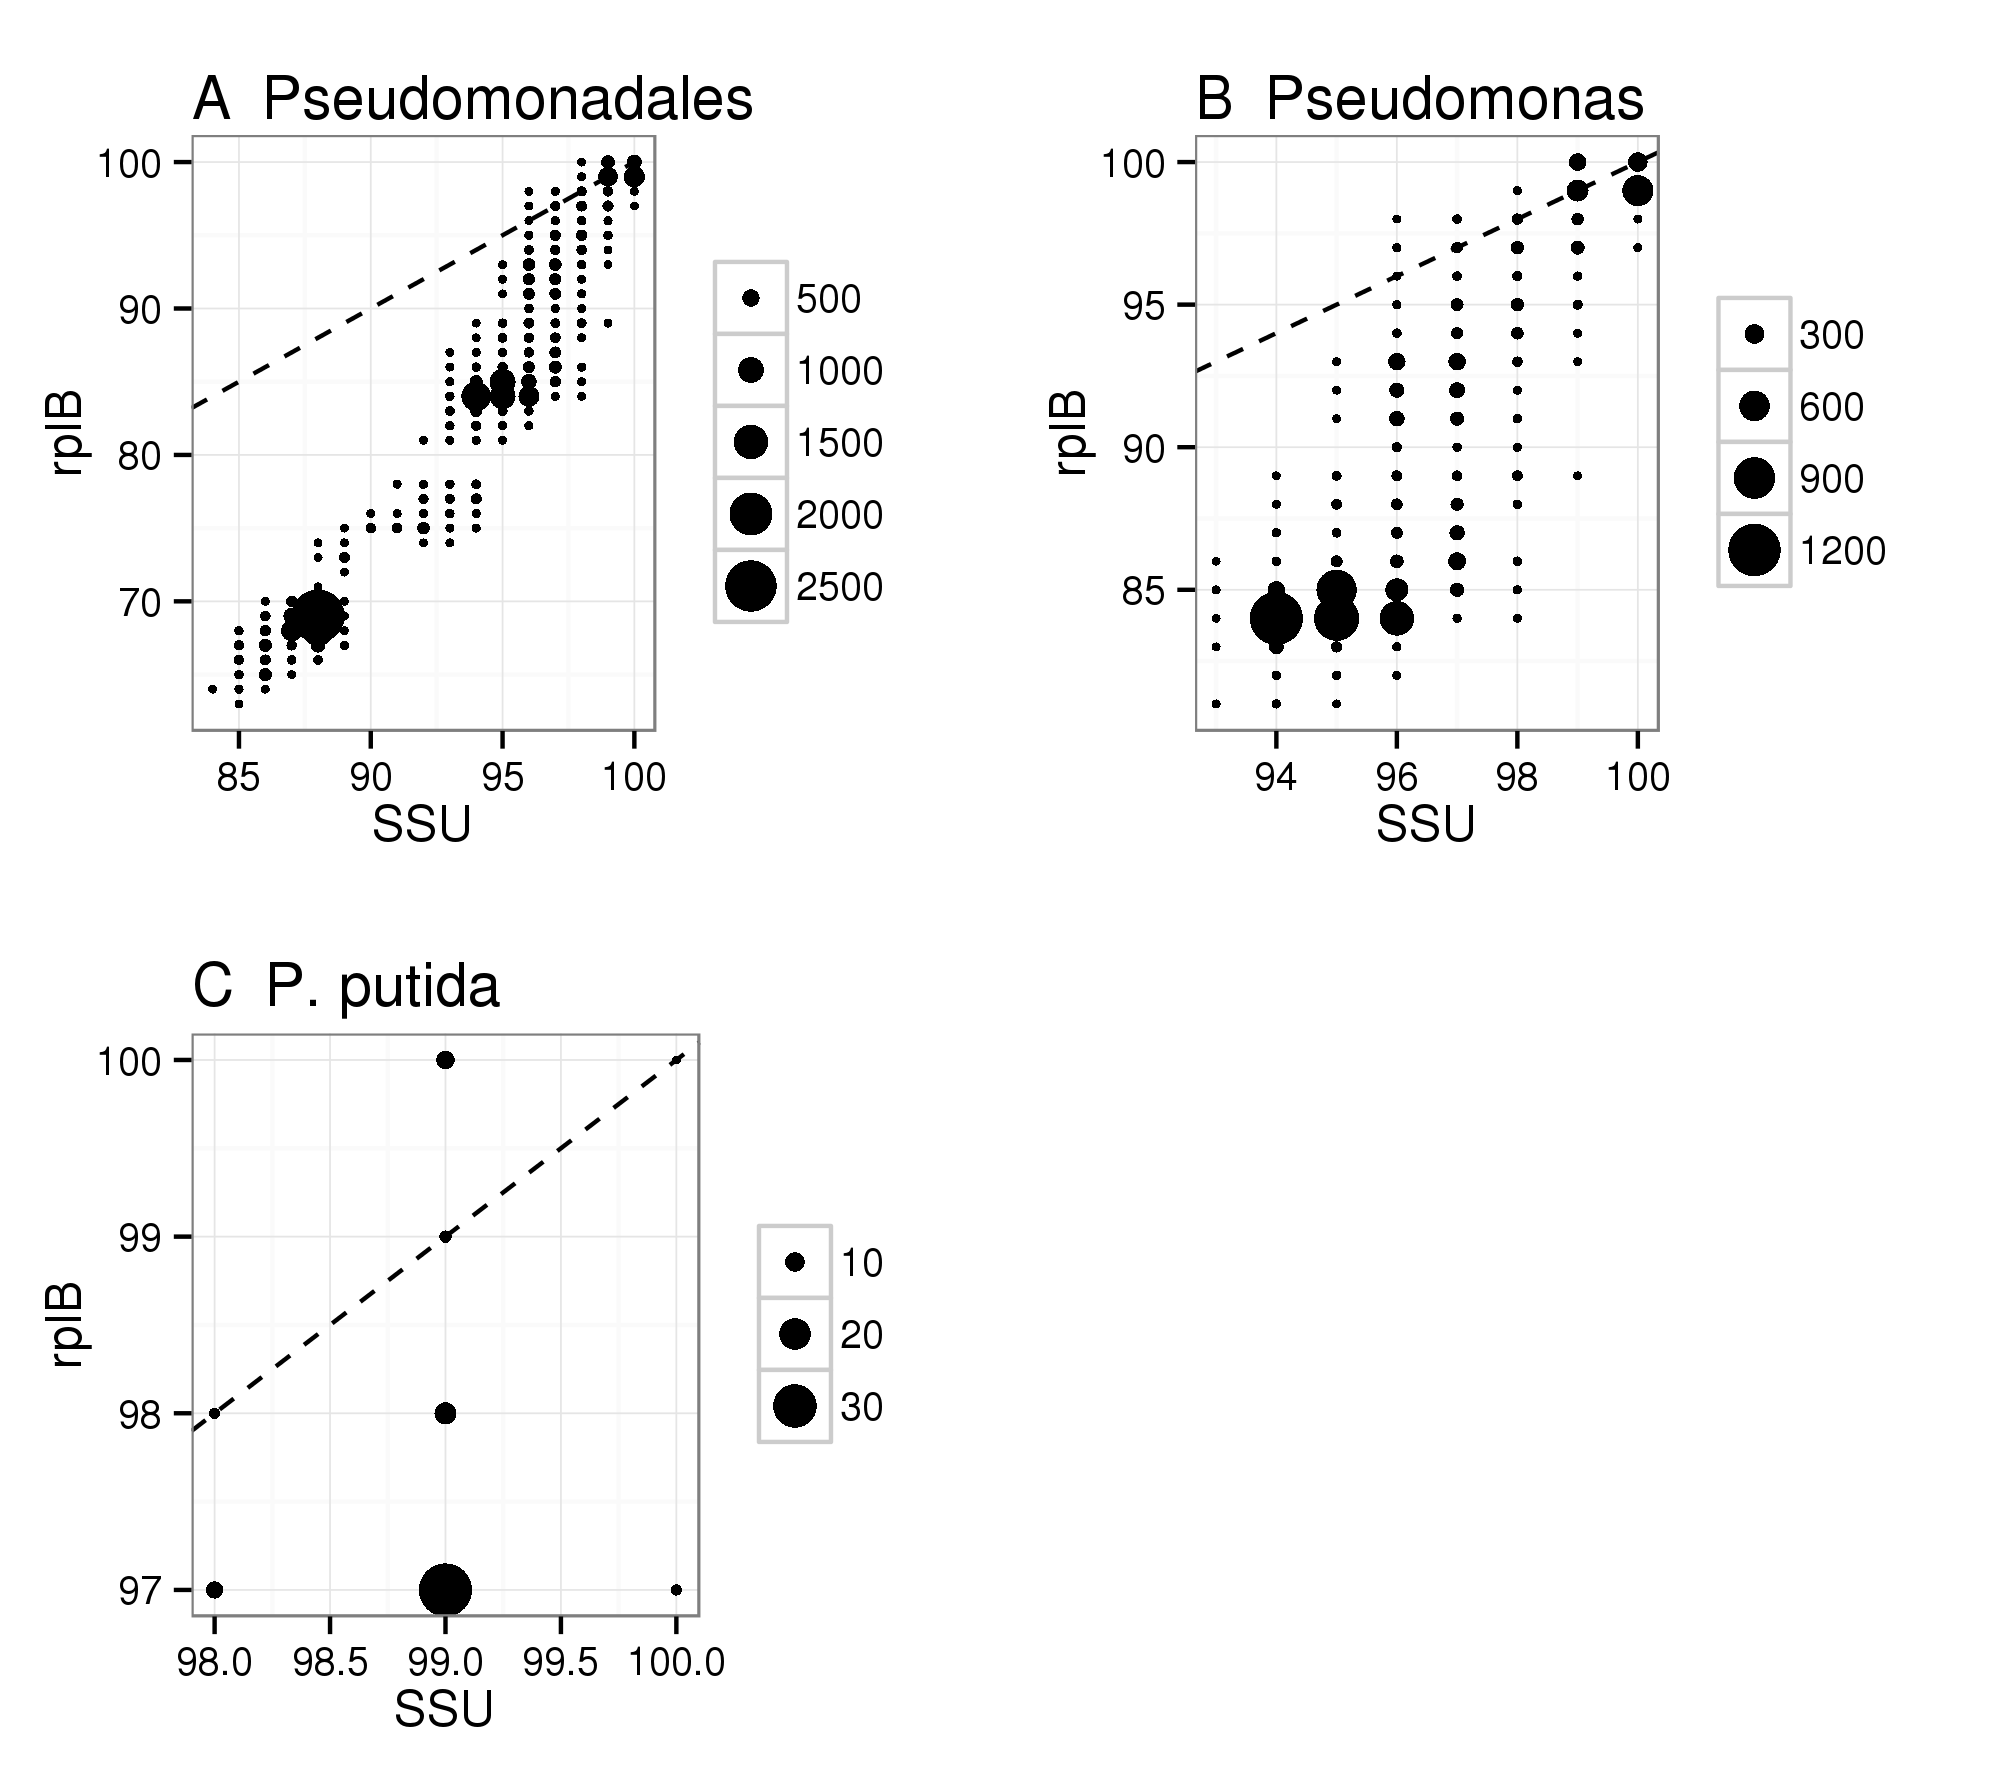
\includegraphics[scale=1]{figs/P_putida}
  \caption[Pairwise comparison among \textit{P. putida} genomes using SSU rRNA gene and \textit{rplB}]{Pairwise comparison among \textit{P. putida} genomes using SSU rRNA gene and \textit{rplB}. SSU rRNA gene identities are larger than \textit{rplB} in most genome pairs. X axis is SSU rRNA gene identities and Y axis is \textit{rplB} identities. The dashed line is y = x. A. All completed genomes in Pseudomonadales are included in pairwise comparison; B. All completed genomes in \textit{Pseudomonas} are included; C. All completed genomes in \textit{P. putida} are included.}
  \label{fig:PPutida}
\end{figure}


\begin{figure}[tbph!]
  \centering
  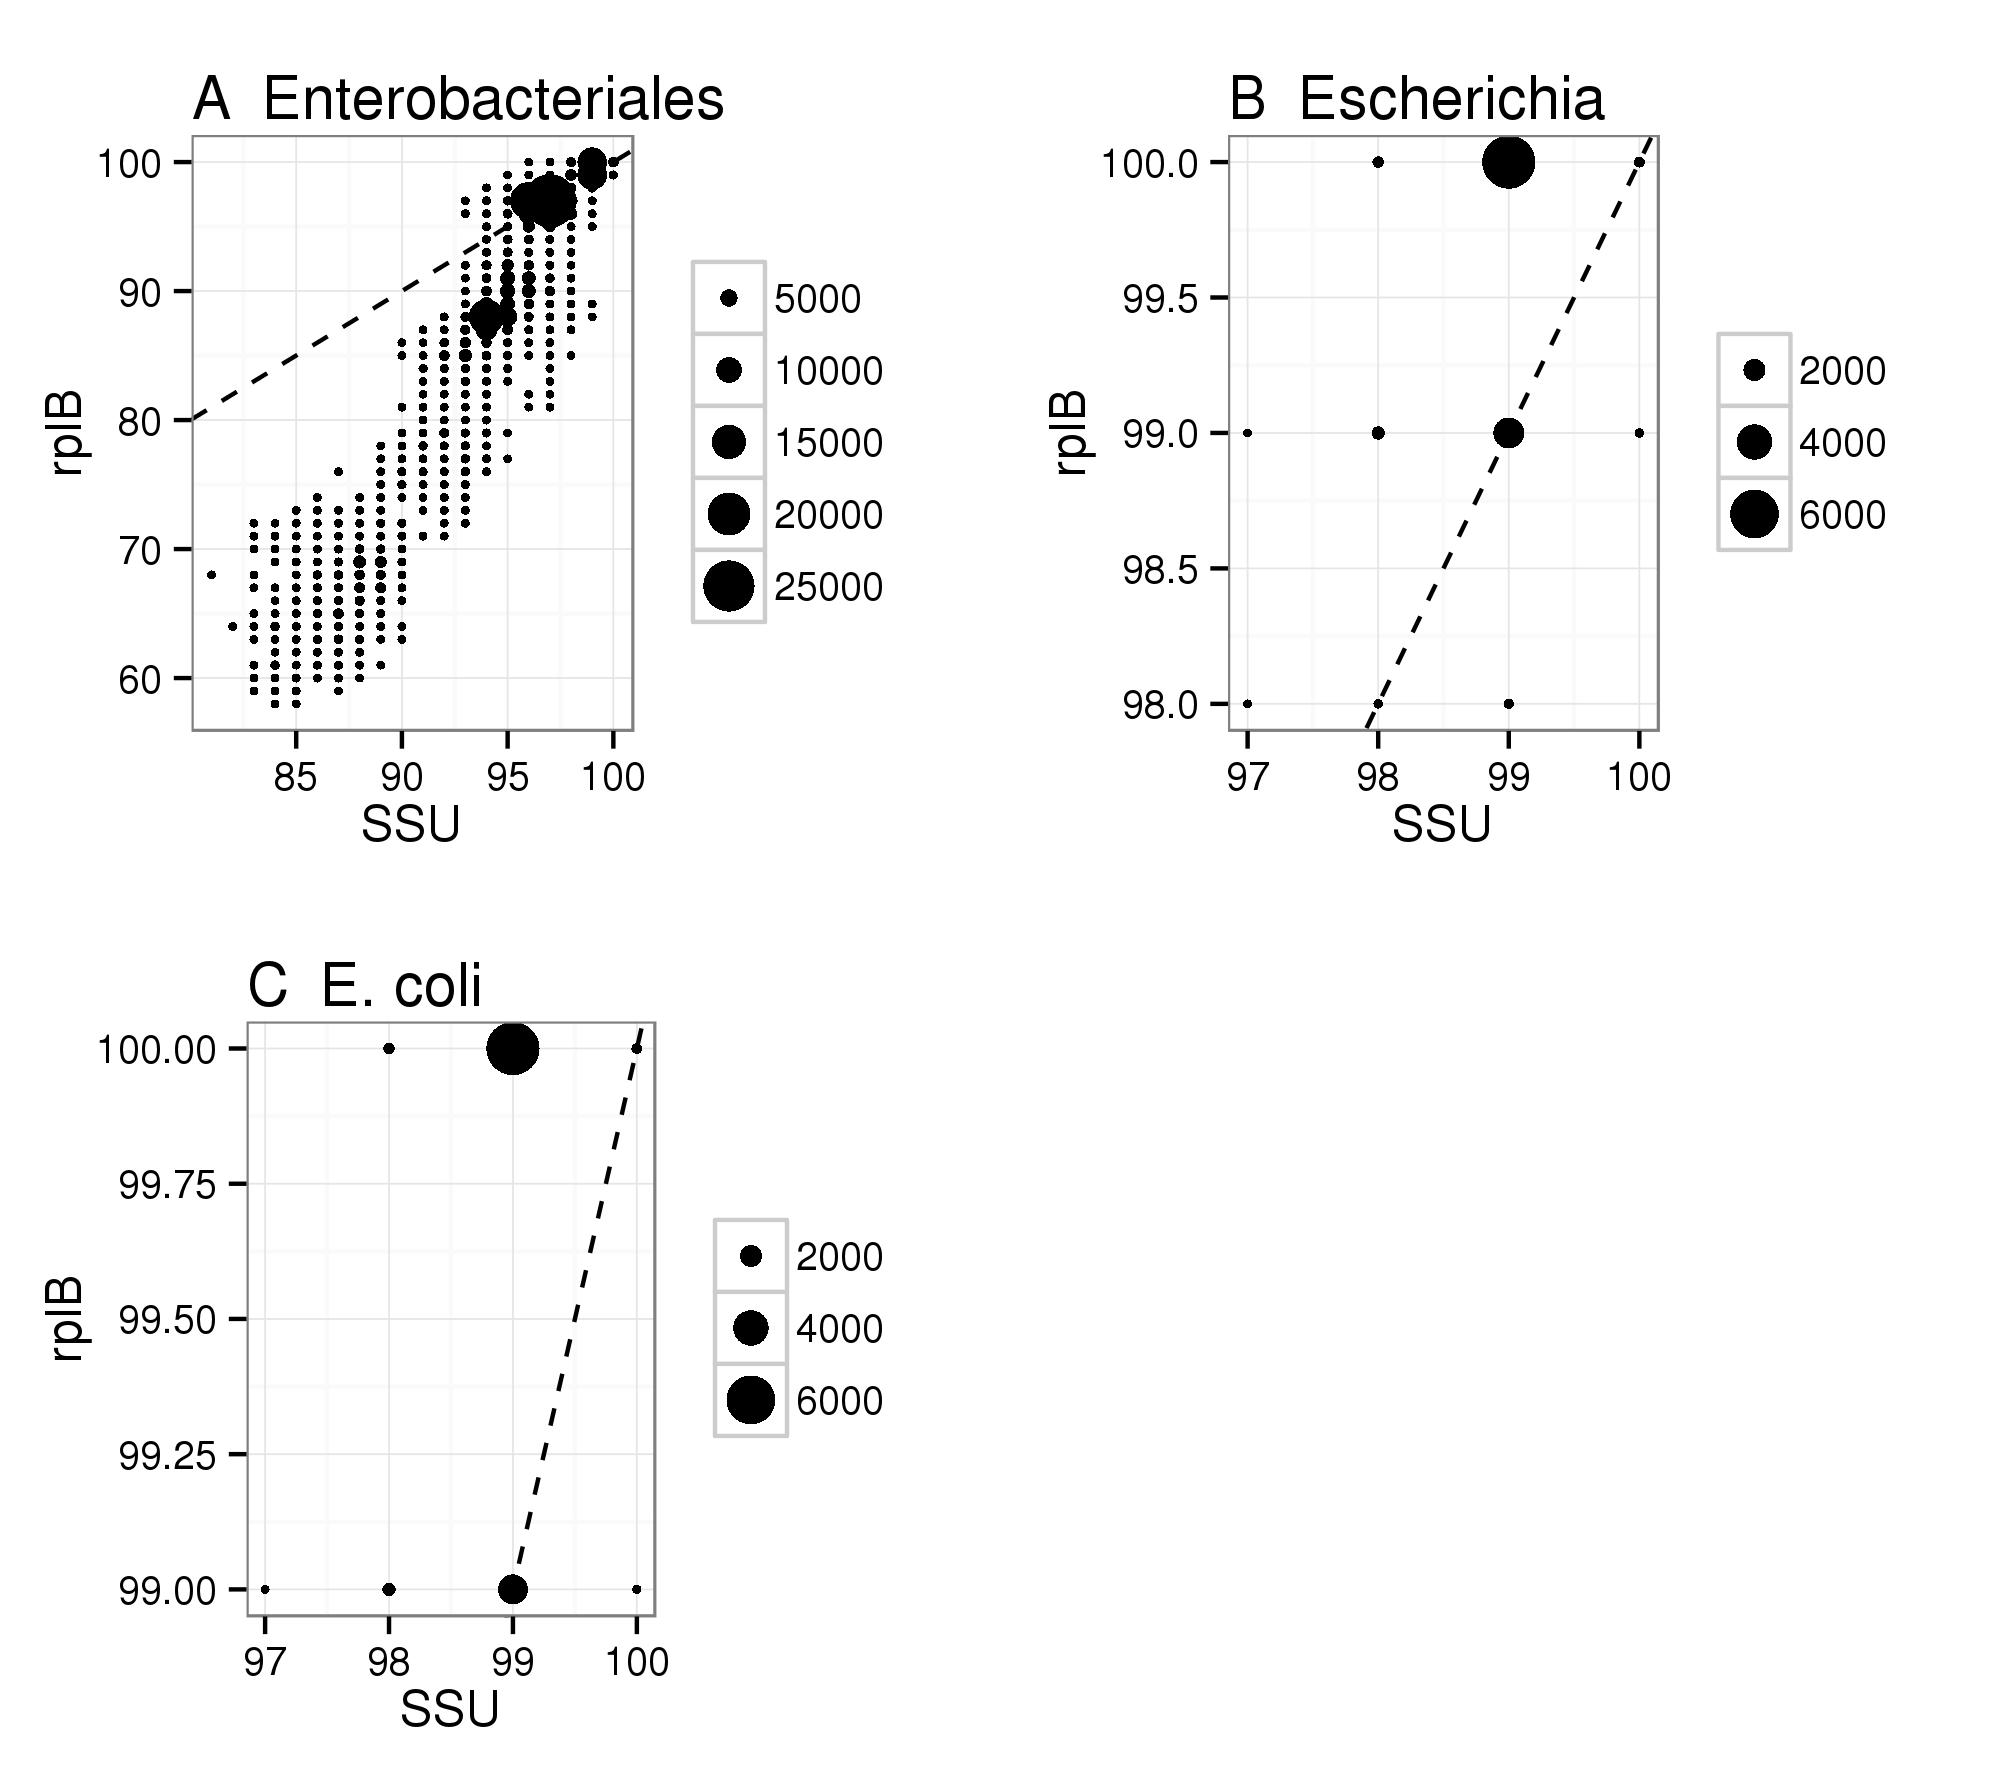
\includegraphics[scale=1]{figs/E_coli}
  \caption[Pairwise comparison among \textit{E. coli} genomes using SSU rRNA gene and \textit{rplB}]{Pairwise comparison among \textit{E. coli} genomes using SSU rRNA gene and \textit{rplB}. X axis is SSU rRNA gene identities and Y axis is \textit{rplB} identities. The dashed line is y = x. A. All completed genomes in Enterobacteriales are included in pairwise comparison; B. All completed genomes in \textit{Escherichia} are included; C. All completed genomes in \textit{E. coli} are included.}
  \label{fig:EColi}
\end{figure}


\begin{figure}[tbph!]
  \centering
  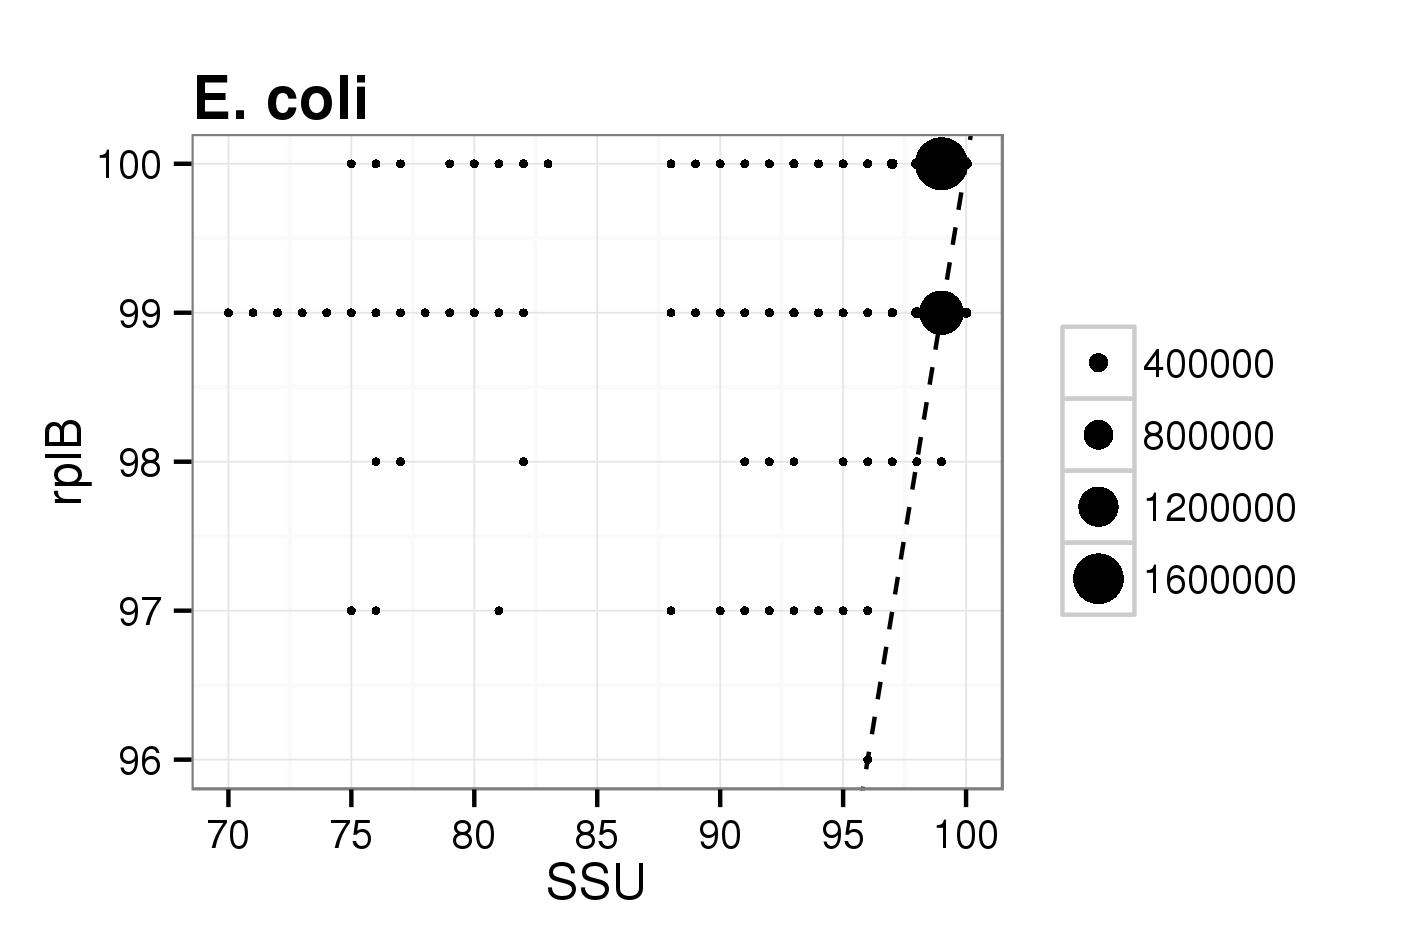
\includegraphics[scale=1]{figs/E_coli_all}
  \caption[Pairwise comparison among all \textit{E. coli} genomes using SSU rRNA gene and \textit{rplB}]{Pairwise comparison among all \textit{E. coli} genomes using SSU rRNA gene and \textit{rplB}. SSU rRNA gene identities are smaller than \textit{rplB} in most genome pairs and some are as low as 70\%. X axis is SSU rRNA gene identities and Y axis is \textit{rplB} identities. The dashed line is y = x. }
  \label{fig:EColiAll}
\end{figure}

\textbf{Comparison of SSU rRNA gene and \textit{rplB} on diversity analyses in large soil shotgun metagenomes. }
On average, 0.04 \% of total reads were identified as SSU rRNA gene fragment and 0.004 \% of total reads were aligned to V4 region of the gene with SSUsearch. Meanwhile, 0.01 \% of total reads were identified as \textit{rplB} with Xander (Table \ref{tab:S3}). Further, we found that SSU rRNA gene consistently had more OTUs than \textit{rplB} with even subsampling in a distance cutoff range of 0 to 10\%. However, after evenly subsampling sequences to 6000 for each gene, we observed \textit{rplB} nucleotide sequences had more OTUs than SSU rRNA gene consistently, and \textit{rplB} protein sequences had less OTUs than SSU rRNA gene in a range of 2 to 5\% but more OTUs than SSU rRNA gene in other distance cutoffs (\cref{fig:otuMetag}). Regardless of the above differences in OTUs resolution, both genes provided the same biological conclusions in two common diversity analyses that the microbial communities in rhizosphere soil of corn were different from those in Miscanthus and switchgrass (beta diversity by ordination) (\cref{fig:pcaMetag}), and corn had a significantly lower diversity than Miscanthus and switchgrass (alpha diversity) (\cref{fig:shannonMetag}). In addition, \textit{rplB} ordination explained larger $R^2$ and \textit{rplB} also separated the microbial communities in Miscanthus and switchgrass while SSU rRNA gene did not, suggesting higher resolution of \textit{rplB} genes (\cref{fig:pcaMetag}).


% Table generated by Excel2LaTeX from sheet 'S3'
\begin{table}[htbp]
  \centering
  \caption[Summary of reads identified as SSU rRNA gene and \textit{\textit{rplB}} in soil metagenomes]{Summary of reads identified as SSU rRNA gene and \textit{\textit{rplB}} in soil metagenomes.}
    \begin{tabular}{|rrrrrrrr|}
    \toprule
          & TotalReads & SSU   & SSU \% & V4    & V4 \% & \textit{rplB}  & \textit{rplB} \% \\
    \midrule
    C1    & 232234095 & 117160 & 0.050\% & 11615 & 0.005\% & 29743 & 0.013\% \\
    C2    & 220844998 & 95493 & 0.043\% & 8137  & 0.004\% & 22605 & 0.010\% \\
    C3    & 282123335 & 119210 & 0.042\% & 11579 & 0.004\% & 33076 & 0.012\% \\
    C4    & 260542662 & 107114 & 0.041\% & 10295 & 0.004\% & 28427 & 0.011\% \\
    C5    & 285873232 & 143302 & 0.050\% & 13520 & 0.005\% & 33428 & 0.012\% \\
    C6    & 250477617 & 124598 & 0.050\% & 12487 & 0.005\% & 29668 & 0.012\% \\
    C7    & 262943930 & 114183 & 0.043\% & 9449  & 0.004\% & 29729 & 0.011\% \\
    M1    & 274060925 & 102049 & 0.037\% & 9693  & 0.004\% & 27210 & 0.010\% \\
    M2    & 278278868 & 100498 & 0.036\% & 9767  & 0.004\% & 28041 & 0.010\% \\
    M3    & 244772969 & 92624 & 0.038\% & 8963  & 0.004\% & 24944 & 0.010\% \\
    M4    & 206129129 & 69535 & 0.034\% & 6474  & 0.003\% & 20777 & 0.010\% \\
    M5    & 225964704 & 74778 & 0.033\% & 6892  & 0.003\% & 22713 & 0.010\% \\
    M6    & 215320045 & 73062 & 0.034\% & 6800  & 0.003\% & 22074 & 0.010\% \\
    M7    & 160726636 & 71249 & 0.044\% & 6580  & 0.004\% & 15182 & 0.009\% \\
    S1    & 192776425 & 68080 & 0.035\% & 6481  & 0.003\% & 19262 & 0.010\% \\
    S2    & 143660127 & 57229 & 0.040\% & 5469  & 0.004\% & 13270 & 0.009\% \\
    S3    & 218743879 & 76368 & 0.035\% & 7210  & 0.003\% & 21421 & 0.010\% \\
    S4    & 249773480 & 78422 & 0.031\% & 7215  & 0.003\% & 23664 & 0.009\% \\
    S5    & 140239637 & 49962 & 0.036\% & 4598  & 0.003\% & 12180 & 0.009\% \\
    S6    & 254749228 & 82105 & 0.032\% & 7282  & 0.003\% & 24364 & 0.010\% \\
    S7    & 194863138 & 68094 & 0.035\% & 6504  & 0.003\% & 19184 & 0.010\% \\
    \bottomrule
    \end{tabular}%
  \label{tab:S3}%
\end{table}%


\begin{figure}[tbph!]
  \centering
  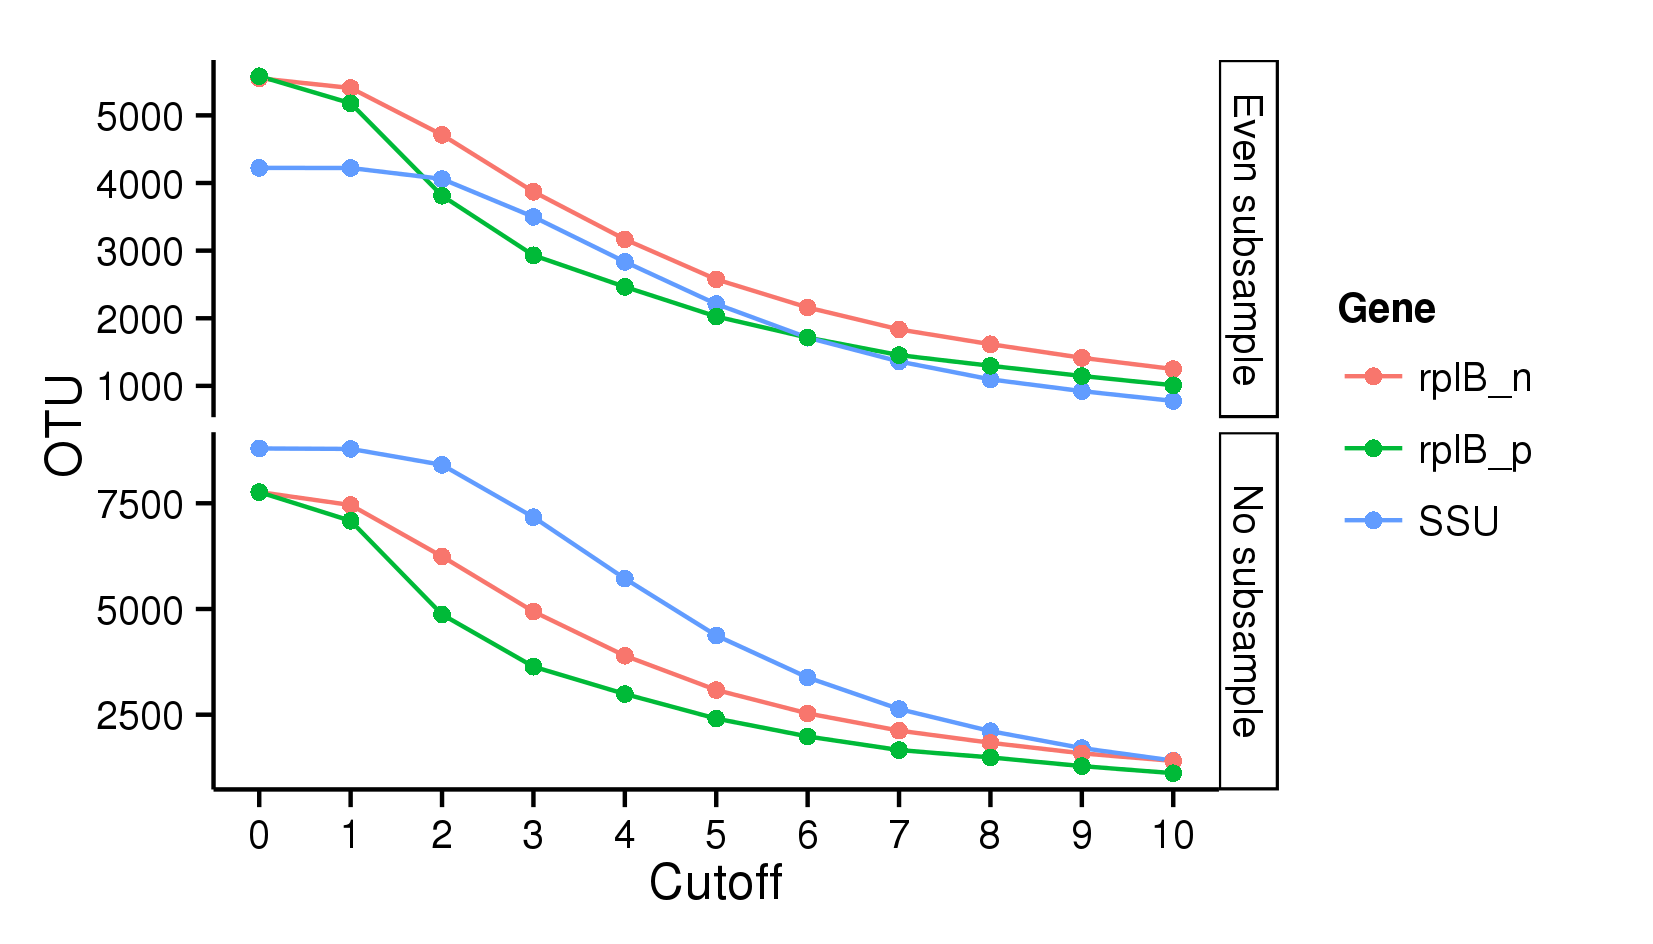
\includegraphics[scale=1]{figs/otu_metag}
  \caption[Comparison of SSU rRNA gene and \textit{rplB} in soil metagenomes]{Comparison of OTU numbers using SSU rRNA gene and \textit{rplB} in large soil metagenomes. The lower panel shows that there are more OTUs using SSU rRNA gene than \textit{rplB} without even sampling, but the upper panel shows that there are less OTUs using SSU rRNA gene after even subsampling. X axis is percentage distance cutoff for OTU clustering and Y axis is OTU number.}
  \label{fig:otuMetag}
\end{figure}


\begin{figure}[tbph!]
  \centering
  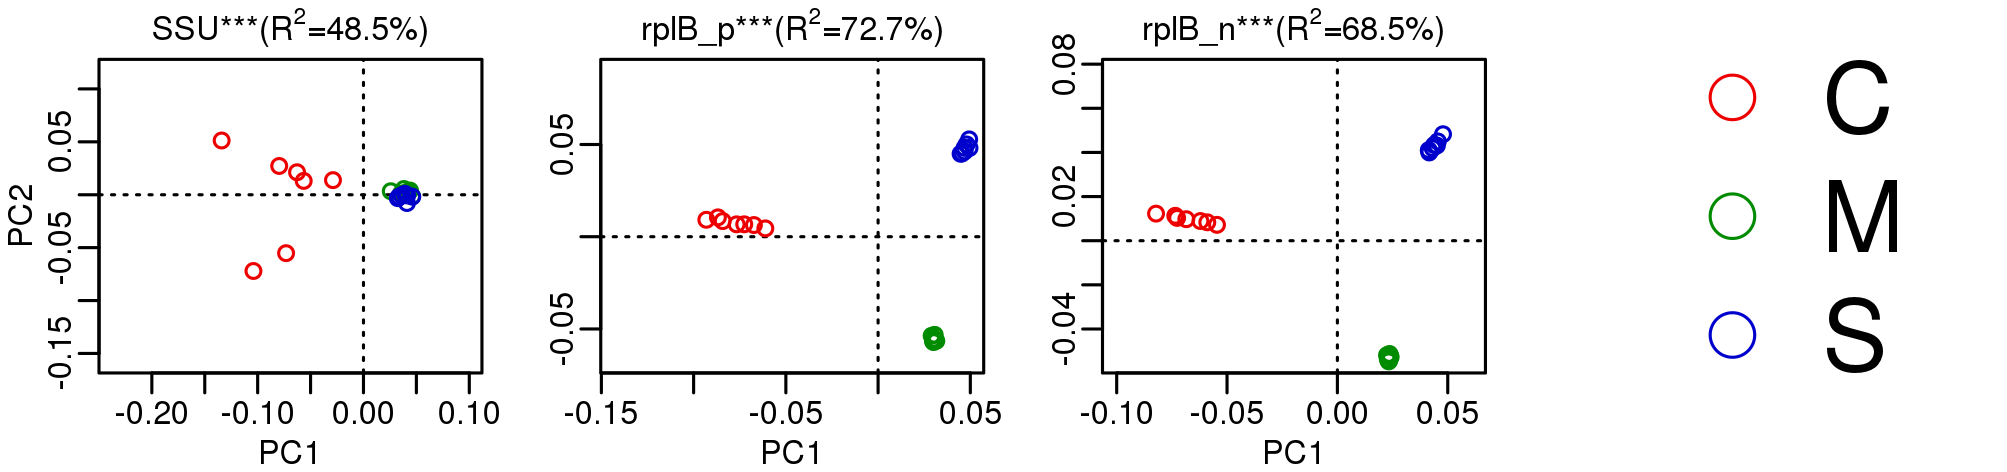
\includegraphics[scale=1]{figs/pca_metag}
  \caption[Comparison of SSU rRNA gene and \textit{rplB} in beta diversity using large soil metagenomes]{Comparison of SSU rRNA gene and \textit{rplB} in beta diversity analysis (ordination) using large soil metagenomes. Both genes show microbial community in corn rhizosphere is significantly different from those in Miscanthus and switchgrass. Additionaly, \textit{rplB} (both nucleotide and protein) also separates microbial communities of Miscanthus and switchgrass, suggesting the higher resolution of \textit{rplB}.}
  \label{fig:pcaMetag}
\end{figure}


\begin{figure}[tbph!]
  \centering
  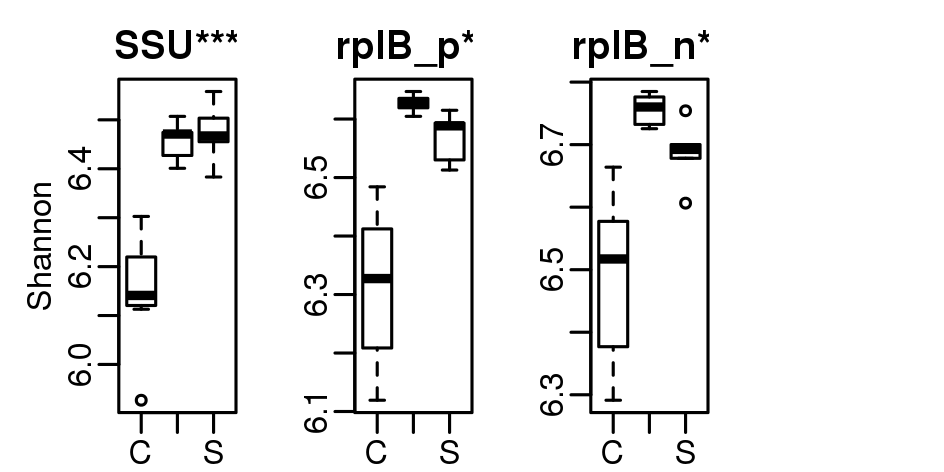
\includegraphics[scale=1]{figs/shannon_metag}
  \caption[Comparison of SSU rRNA gene and \textit{rplB} in alpha diversity using large soil metagenomes]{Comparison of SSU rRNA gene and \textit{rplB} in alpha diversity analysis (Shannon diversity index) using large soil metagenomes. Both genes show microbial community in corn rhizosphere is significantly less diverse than those in Miscanthus and switchgrass.}
  \label{fig:shannonMetag}
\end{figure}


\section{Disscussion}

Although single phylogenetic marker based species definition are limited compared to whole genome based species definition, it still is the most effective and practical approach for microbial community analyses. Here we compare a single copy protein coding gene (\textit{rplB}) with the commonly used SSU rRNA gene and demonstrate that single copy protein coding gene are suited for community species diversity analyses using all baterial genomes and large soil shotgun metagenomes.

\textbf{Choosing genomic datasets. }
For the comparison of \textit{rplB} and SSU rRNA gene with genomes, genome (assembly) quality is critical because erroneous sequences of SSU rRNA genes and \textit{rplB} extracted from low assembly quality genomes could lead to problematic results. Meanwhile, we also intend to include as many genomes as possible to make the conclusion more generalizable. We choose from two sets of genomes. The first set are only completed genomes (4457), which are supposed to have higher quality. The second set are larger with all the Bacterial genomes (53865), most of which are not completed (with fragmented contigs). The facts that the second set has higher ratio of genomes with \textit{rplB} copy number more than one, and many \textit{E. coli} strains in the second dataset shows lower than 80 \% similarity in SSU rRNA genes (\cref{fig:EColi}) indicates some poor genome assemblies in the second set. Thus we pick the first set (completed genomes) for further analyses. Short reads sequencing technology has made sequencing bacterial genomes cheaper than faster but also make finishing a genome not cost effective so most assembled genomes are not complete \cite{land_insights_2015}. Especially for genomic regions with multiple copy such as SSU rRNA gene, assembly from short reads are prone to assembly error and long reads are needed to solve the problem.

\textbf{Advantages of \textit{rplB} over SSU rRNA gene as a phylogenetic marker. }
First, SSU rRNA gene (a multiple copy gene) post difficulties on interpreting species (OTU) abundance since abundance of species with multiple copies of SSU rRNA gene are inflated, while \textit{rplB} (a single copy gene) does not has the same issue. Additionally, the variation among multiple copies can cause multiple OTUs from the same species by sequence clustering \cite{sun_intragenomic_2013} and thus overestimation of species richness. Futher, the number of \textit{rplB} genes in a community represents the number of microbial cellls, which makes \textit{rplB} suitable for normalizing abundance of other genes (portion of cells with that gene).
Second, SSU rRNA gene are also more prone to assembly errors (chimera) than single copy genes due to multiple copies and variation among copies, which is also consistent with the results that there are unexpectedly low similarities (< 80 \%) observed among SSU rRNA genes of \textit{E. coli} strains while \textit{rplB} has high similarities (> 95 \%) among \textit{E. coli} strains when incompleted genomes are included (\cref{fig:EColiAll}). Note that these erroneous sequences would be further collected by databases such as RDP and SILVA \cite{cole_ribosomal_2014,quast_silva_2013} and used as references for taxonomy, alignment, and chimera detection, and thus have a impact on common microbial ecology diversity analyses, so switching to a single copy gene that are less prone to assembly error can mitigate the above problem.
Third, we have shown \textit{rplB} has a higher resolution to differentiate closely related species than SSU rRNA gene, supported by the results that \textit{rplB} having larger distance than SSU rRNA gene in pairwise comparison of the genomes (\cref{fig:interSpeciesComp,fig:RLeg,fig:PPutida,fig:EColi}) and also there are more OTUs clusterd with \textit{rplB} nucleotide sequences than SSU rRNA gene in soil shotgun metagenomic data (\cref{fig:otuMetag}). This is consistent with the crucial role SSU rRNA play in translation as part of ribosome (ensuring translation accuracy and working with LSU rRNA to process the mRNA a codon a time) \cite{carter_functional_2000}, which is also confirmed by another study showing SSU rRNA gene (along with LSU rRNA gene, tRNA and ABC transporter genes) has been reported to be the most conserved genes \cite{isenbarger_most_2008}. Since \textit{rplB} sequences are compared at nucleotide space, the synonymous mutations at the third positions of codons in \textit{rplB} also explain its higher resolution. Further, the heterogeneity among copies of SSU rRNA gene in the same genome can be higher than those among different species \cite{sun_intragenomic_2013}, which means SSU rRNA gene is not suitable to resolve lower taxonomies such as species and strains.
At last, \textit{rplB} also has the advantage of having sequences in both nucleotide space and protein space. Higher level taxonomies can be resolved at protein space, while lower level taxonomies can be resolved at nucleotide space with protein sequences guiding the nucleotide sequences to get more accurate alignment (codon alignment), which is critical for phylogenetic analysis and multiple sequence alignment based OTU clustering.

\textbf{Novelties in this study. }
Althought there are other studies on comparing single copy housekeeping gene and SSU rRNA gene \cite{case_use_2007,roux_comparison_2011}, the novelty in our analyses is that we use OTU (from \textit{de novo} clustering), which is more common than taxonomy in microbial diversity analyses and enabled by recent advancement in shotgun metagenomic analysis methodology, SSUsearch and EMIRGE (for SSU rRNA gene) \cite{guo_microbial_2015,miller_short-read_2013} and Xander (for \textit{rplB}) \cite{wang_xander:_2015}. In contrast, the other studies do comparion at taxonomy level, which is problematic because many reads can not be classified high confidence due to lack references and thus be dicarded, especially for genes other than SSU rRNA gene. Second, we compare these two genes with much larger genomic data and larger shotgun metagenomic data. For example, Case et al. compared rpoB (beta subunit RNA polymerase) with SSU rRNA gene using only 111 completed genomes from NCBI \cite{case_use_2007}, while we include 4457 completed genomes, which require orders of magnitudes higher computation to extract the genes and do pairwise comparison and more importantly can result in more generalizable conclusion. Similarly with shotgun metagenomic data, Roux et al. do the comparison using a subset of shotgun metagenomes from Global Ocean Survey, which is about six billion bp in total from sanger sequencing \cite{roux_comparison_2011,rusch_sorcerer_2007}, while our soil metagenomic datasets are about 900 billion bp in total. 


\textbf{Lower strain level resolution of SSU rRNA gene due to its intra-genome variations. }
Additionally, we find inconsistent results when comparing two genes at strain level with different species (\cref{fig:RLeg,fig:PPutida,fig:EColi}). The exception in \textit{E. coli} could be explained by the intra-genome variations of SSU rRNA gene (\cref{fig:intraGenome3species}) that lead to larger inter-strain variation than \textit{rplB} among strains, which could not be interpreted as better resolution. Consistently, we observed OTU number from SSU decrease slower when distance cutoff is less than 4\% (slope of line in \cref{fig:otuMetag}), which causes OTU number of SSU rRNA gene to be higher than \textit{rplB} protein and suggests that intra-genome variation of SSU rRNA gene are causing inflation of OTU numbers \cite{sun_intragenomic_2013} and also make SSU rRNA gene not suitable for strain identification.

\textbf{Comparison of two genes in \textit{de novo} OTU based community diversity analyses. }
Another goal of this study is to evaluate the effect of two different genes on common OTU based diversity analyses such as alpha diversity and beta diversity. Other than more OTUs result from \textit{rplB} nucleotide sequences than SSU rRNA gene using the same distance cutoff (0.03), diversity analyses of two genes provide the same biological conclusion except that \textit{rplB} also separates Miscanthus and switchgrass while corn does not, suggesting \textit{rplB} has higher resolution than SSU rRNA gene. This is similar to comparison of taxonony (phylotype in mothur term) based diversity analysis and \textit{de novo} OTU based diversity analyses. Although species or genus level is enough to differentiate the biological treatments sometimes, higher resolution levels (OTU) are still preferred when the differences are not obvious, e.g. there are not difference in community composition at species level but strain composition in some species are different. For the same reason, higher varition in \textit{rplB} make the gene a better phylogenetic marker than SSU rRNA gene for analyzing more similar communities.

\textbf{Sequencing depth needed for \textit{rplB} in metagenomes. }
Now that \textit{de novo} OTU based diversity analyses with \textit{rplB} in shotgun metagenomes have been enabled by Xander, another common question in experiment design is that how much sequencing are needed to ensure there is enough coverage on \textit{rplB} gene for diversity analyses. Saturation of OTU from \textit{rplB} sequences is difficult due to high microbial diversity in soil and sequencing error and also not necessary for beta-diversity analysis (add REF), so an empirical fold coverage 3000 is recommended for soil samples based on experiences with SSU rRNA gene (add REF, SSUsearch), which means about 25 Gbp (3000*850 bp/0.01\%) shotgun sequences are needed with 850 bp as the average length of \textit{rplB} and 0.01\% as average portion of total for \textit{rplB} (Table \ref{tab:S3}).

{Lack of universal primers for amplification and reference sequences. }
There are a few drawbacks of single copy housekeeping genes such as \textit{rplB}. First, the high varition among gene sequences especially the high mutation rate at the third position of codon makes it difficult to design universal primers. Although new methods for analyzing shotgun metagenomes enable us to avoid primer amplification \cite{guo_microbial_2015,wang_xander:_2015,miller_short-read_2013}, the cost of shotgun sequencing on large number of samples with decent sequencing depth as mentioned above is still high and thus a limitation. Therefore, availability of universal primers are still desirable traits for a good phylogenetic marker. Second, \textit{rplB} and other single copy housekeeping genes lack reference sequences, while SSU rRNA gene has accumulated large amount of reference sequences, as such those in RDP and SILVA \cite{cole_ribosomal_2014,quast_silva_2013} that are critical for diversity analyses.

\section{Conclusion}

Although genome level comparison has the highest resolution to identify species and strains, phylogenetic marker is still essential for community diversity analysis. We demostrate that \textit{rplB}, a single copy protein coding gene, can provide finer resolution to identify low level taxonomy such as species and strains than SSU rRNA gene (\cref{fig:interSpeciesComp}) and also finer scale (OTU) diversity analysis (\cref{fig:otuMetag,fig:pcaMetag}). In spite of the lack of references, more references will become available with bacterial genome sequencing becomes faster and cheaper \cite{land_insights_2015}. Thus single copy protein coding genes such as \textit{rplB} have great potential to complement or even replace SSU rRNA gene as a phylogenetic marker. 


\chapter{Rhizosphere metagenomics of three biofuel crops}
%
% If you have pages that must appear in landscape mode, use the [lscape] option
% and enclose the pages in a {landscape} environment.
%\clearpage\pagestyle{lscape} % first clear the page and change the pagestyle
%\begin{landscape}
%
% your landscape table(s) or figure(s) here
%
%\end{landscape}
%\pagestyle{plain} % remember to change the pagestyle back to plain
%
%
% If you have appendices, they would go here.  
% Comment these lines out if you don't
% If you have more than one appendix, you need to use 
%   \begin{appendices}
%   \chapter{First appendix}
%   \chapter{Second appendix}
%   \end{appendices}
%


\begin{abstract}
Soil microbes form beneficial association with crops in rhizosphere and also play a major role in ecosystem functions, such as N and C cycle. Crop roots had strong influences on the soil microbial community. Thus large-scale plantation of biofuel crops will have significant impact on ecosystem functions regionally and beyond. We compared rhizosphere microbial communities of corn (annual) and switchgrass and Miscanthus (perennials). This is the first comparative study of these biofuel crops using shotgun metagenomics and one of the largest sequencing efforts to date (about 1 TB bp in total). We compared the rhizosphere metagenomes at three levels: overall community structure (SSU rRNA gene), overall function (annotation from global assembly), and N cycle genes (from Xander). All three levels showed corn had a significantly different community from Miscanthus and switchgrass (except for AOA). In terms of life history strategy, the corn rhizosphere was enriched with more copiotrophs while the perennials were enriched with oligotrophs, which is further supported by higher abundance of genes in “Carbohydrates” and higher fungi/bacteria ratios. In addition, corn also had a less rich and even community, so the perennials managed to maintain a more diverse community even though investing less C in the rhizosphere. Moreover, a larger dispersion of corn data in ordination plots and enriched Penicillium (non-beneficial fungi) also indicate corn may not be doing as well in controlling its community and selecting beneficial member. Furthermore, the nitrogen fixing community of corn was dominated by \textit{Rhizobium} (perhaps a legacy from prior legume crops) while the perennials had NifH sequences most related to \textit{Coraliomargarita}, \textit{Novosphingobium} and \textit{Azospirillum}, indicating that the perennials can better select beneficial members. Moreover, higher numbers of genes for nitrogen fixation and lower number of genes for nitrite reduction suggest better nitrogen sustainability of the perennials. Thus our study provides comprehensive evidence showing perennial bioenergy crops have advantages over corn in higher microbial species and functional diversity and in selecting members with beneficial traits, consistent with a higher level of sustainability of perennial biofuel crops.
\end{abstract}

\section{Introduction}

Bioenergy is green energy, but growing bioenergy crop is not fully environmental friendly. Bioenergy crop growth requires energy inputs (fertilizer and pesticides), emits greenhouse gases (N2O), and competes with food production for land \cite{crutzen_n2o_2008}. Rhizosphere (interface between plant roots and soil) is an important part of the soil where microbes and plants form beneficial associations, where plants give microbes C source and microbes provides plant nutrients (N and P), growth hormone, and disease resistance \cite{bulgarelli_structure_2013,baudoin_impact_2003,dennis_are_2010}. Thus rhizosphere microbial community has the potential reduce the cost of growing bioenergy plants (less fertilizer and pesticide usage) and is key for sustainability, especially when we grow bioenergy crops in marginal land that is not optimal for the crops.

Vegetation has strong influence on microbial community structure through the root exudates and detritus, the primary carbon and energy source for soil microbes. Nevertheless, their influence varies depending on the plant species and ecosystem types \cite{smalla_bulk_2001,mao_changes_2011}. Here we studied the rhizosphere of three common biofuel crops (corn, Miscanthus and switchgrass) from the same family (true grasses) but varies in phenotype. Miscanthus and switchgrass are perennial grasses with fibrous roots, while corn is an annual with less fibrous root. Miscanthus is the largest in size and originated from tropical regions, while switchgrass is native in Midwest, US. Large scale planting of these biofuel crops may change soil microbial community structure and function, and impact global nutrient cycle processes such as N cycle. Corn typically needs fertilizer to grow, and the N fertilizers are reported to cost about 40\% of total energy input \cite{camargo_energy_2013}. On the other hand, Miscanthus and switchgrass can grow with little or no N fertilizer \cite{schwarz_effect_1994,mao_impact_2013,parrish_biology_2005}, so the perennial grasses are thought to have better nitrogen sustainability. It is still not known that how much rhizosphere microbes contribute to the better nitrogen sustainability of perennials since nutrient translocation before senescence and phyllosphere (leaf) microbes are also possible cause. Here we not only study the overall microbial community diversity of three biofuel crops but also focus on groups involved in N cycle. We hypothesize that the rhizosphere microbial communities of perennials are adapted to a low N environment and have increased N fixation, and decreased nitrification and denitrification.

Despite limited understanding of rhizosphere microorganisms, the chemistry of the nutrient cycles carried out by those microorganisms is relatively clear, including nitrogen fixation, nitrification, and denitrification. Nitrogen fixing microbial community is commonly measured with nifH as marker and nitrifying community is commonly measured with AOA (archaeal amoA) and AOB (bacterial amoA) \cite{gaby_comprehensive_2012,prosser_archaeal_2012}. Denitrification has multiple steps including nitrate reduction (Nar), nitrite reduction (Nir), nitric oxide reduction (Nor) and nitrous oxide reduction (Nos). Nir has two types, Cu-Nir (copper based) and cd1-Nir (iron based), encoded by nirK and nirS respectively. Nor has cNor (with cytochrome c) and qNor (without cytochrome c). Nos also has different types, encoded by typical nosZ (clade I) and atypical nosZ (clade II) \cite{zumft_cell_1997}. Thus amplicon based studies only targeting one single type of a gene for nitrification and denitrification may underestimate abundance of microbes involved.

Most surveys on N cycle related communities in soils use amplicon based methods \cite{mao_impact_2013,hai_quantification_2009,kandeler_abundance_2006}, which has primer bias problem, especially for those N cycle genes that lack well curated reference databases \cite{gaby_comprehensive_2012,sanford_unexpected_2012,heylen_incidence_2006}. Shotgun metagenomic method produces short reads fragments representing all the genetic information of community members and thus has no primer bias. The new challenge coming with the shotgun approach is analysis of big data and short read \cite{qin_human_2010,pell_scaling_2012}. There is a cross-disciplinary study showing the perennial grass can increase biodiversity across multiple taxa and enhance multiple ecosystems, but only methanotrophic bacteria is measured within microbiome \cite{werling_perennial_2014}. Our study covers overall microbial diversity and also subgroups involved in N cycle that are of great economic and environmental interest, and thus provides a more complete view of the microbiome. Further, we expect to see stronger microbial response by using rhizosphere soil (< 1 mm to root) rather than bulk soil used in others similar studies \cite{mao_impact_2013,werling_perennial_2014}.

In this study, we applied shotgun metagenomics (about 1 TB DNA data in total) in combination with ecology theory (life history strategy) to study rhizosphere microbial species and functional response to three different crops (corn, Miscanthus, and switchgrass). We use computationally efficient methods to assemble globally (khmer) \cite{pell_scaling_2012,zhang_these_2014,crusoe_khmer_2015} and also extract genes of interest (SSUsearch and Xander) \cite{guo_microbial_2015,wang_xander:_2015} in the big soil shotgun sequencing data. Comparative metagenomics is applied at whole community species and function level and also N cycle gene level to understand microbial responses to different bioenergy crops. 

\section{Methods}

\textbf{Soil samples, DNA extraction, and sequencing.} Rhizosphere samples of corn, switchgrass and Miscanthus were collected at Great Lake Bioenergy Research Center (GLBRC) intensive Cropping System Comparison site in Kellog Biological Station (KBS) (42.394828, -42.394828) (\url{http://data.sustainability.glbrc.org/pages/1.html}) in Michigan on 10/12/2012. We sampled rhizosphere of each crop at seven plot areas. Each replicate was a composite of two or three plant close to the sampling spot. Roots were shaken vigorously to remove loosely attached soil, then cut off from stem and placed in plastic bags 4 degrees C. Soil closely attached to roots (< 1 mm) were collected and washed off roots as rhizosphere soil in lab (Fig. S1). Soil left were send to measure soil chemistry. DNA was extracted with PowerSoil DNA Isolation Kit from MO BIO, USA as described in \cite{jesus_influence_2015} and then sent to Joint Genome Institute (JGI) for Illumina HiSeq 2500 sequencing (250 bp insert libraries and 2 x 150 bp reads).

\begin{figure}[tbph!]
  \centering
  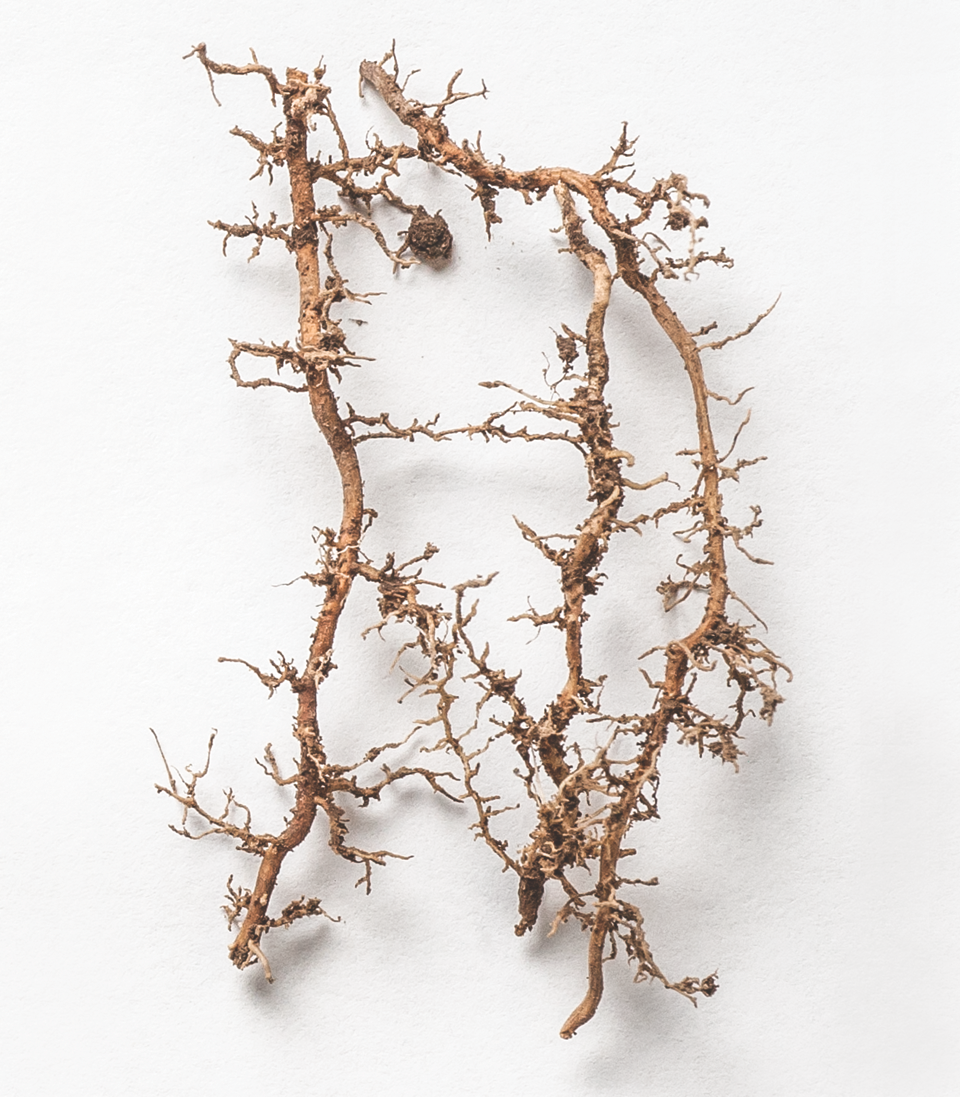
\includegraphics[width=0.80\textwidth]{figs/chap4-root-M}
  \caption[Roots (Miscanthus) and rhizosphere soil]{Roots (Miscanthus) and rhizosphere soil. Rhizosphere soil is collected by washing soil from the roots. The image shows that soil is very close (< 1 mm) to small roots.}
  \label{fig:chap4FigS1}
\end{figure}


\textbf{Data preprocessing. }
Raw Illumina reads were quality trimmed using fastq-mcf (version 1.04.662, \url{http://code.google.com/p/ea-utils}) with flags ``-l 50 -q 30 -w 4 -x 10 –max-ns 0 -X''. Then paired ends were merged by FLASH (version 1.2.7) \cite{magoc_flash:_2011} using flags ``-m 10 -M 120 -x 0.20 -r 140 -f 250 -s 25'' \cite{guo_microbial_2015}.

\textbf{Diversity analysis using SSU rRNA gene. }
SSU rRNA gene fragments in shotgun metagenome are identified and an OTU table was made using fragments aligned to a 150 bp region of V4 (Escherichia coli position 577 to 727) by SSUsearch pipeline \cite{guo_microbial_2015} following a tutorial in \url{https://github.com/dib-lab/SSUsearch}. Ordination, richness and diversity analysis were calculated by phyloseq \cite{mcmurdie_phyloseq:_2013}, simba \cite{jurasinski_simba:_2012} and vegan \cite{oksanen_vegan:_2015} package in R \cite{r_core_team_r:_2014}.

\textbf{Global metagenome assembly, annotation and functional diversity. }
Preprocessed reads of each crop were pooled and then assembled with digital normalization (-k 20 -C 10 -N 4 -x 2.14e11) and partitioning (-k 20 -N 4 -x 6e11) pipeline \cite{howe_tackling_2014} following a tutorial in \url{http://nbviewer.jupyter.org/github/ngs-docs/ngs-notebooks/blob/master/ngs-71-hmp-partition.ipynb} and \url{http://nbviewer.jupyter.org/github/ngs-docs/ngs-notebooks/blob/master/ngs-71-hmp-partition.ipynb} using khmer (version 0.6.1). The partitioned data were then assembled with velvet (version 1.2.08) \cite{zerbino_velvet:_2008} and SGA (version 0.9.35) \cite{simpson_efficient_2012}. For velvet, kmer size of 29, 39, 49, 59 and 69 were used and final assembly was merged with SGA. For SGA, overlap size of 29, 39, 49, 59, and 69 were used and final assemblies were clustered using cd-hit-est (-c 0.99) in CD-HIT \cite{li_cd-hit:_2006}. Contigs shorter than 300 bp were discarded. Since velvet and SGA produced very similar assembly in terms of total size and longest contigs. The assembly from SGA was chosen for further analysis.

The assembly was then uploaded to MG-RAST \cite{meyer_metagenomics_2008} for gene calling and annotation. Gene calling files (with suffix .genecalling.coding.faa), clustering files (with suffix .cluster.aa90.mapping), and BLAT \cite{kent_blatblast-like_2002} tabular output files (with suffix .superblat.sims) were downloaded. BLAT hits with alignment longer than 30 amino acids, identity higher than 70\%, and E-value lower than 0.00001 were used for downstream analysis. Number of hits to each reference in MG-RAST M5NR database for each sample was summarized based on BLAT hits, gene calling IDs, and clustering info. Then M5NR IDs were converted into subsystem IDs and further subsystem ontologies using MG-RAST API (\url{http://api.metagenomics.anl.gov/api.html}). At the end, a count table of subsystem ontologies across each sample was made. Level 3 and Level 1 subsystem were used for ordination analysis with R phyloseq package \cite{mcmurdie_phyloseq:_2013}. For enrichment analysis, group\_significance.py in QIIME \cite{kuczynski_using_2012} was used to find level 3 subsystems (pathways) that significantly different between two crops (p < 0.05, n = 7) and those pathways with more than 10 total counts in all samples and a fold change less than 2/3 or larger than 3/2 were treated as significant.

\textbf{N cycle gene assembly and diversity. }
Preprocessed reads of the same crop were combined and used as input to Xander (gene targeted metagenomic assembler) \cite{wang_xander:_2015} with MAX\_JVM\_HEAP=300G, FILTER\_SIZE=40, K\_SIZE=45, genes=``nosZ nosZ\_a2 nirS amoA\_AOA amoA\_AOB norB\_cNor norB\_qNor'' following tutorial in \url(https://github.com/rdpstaff/Xander\_assembler). Output files with taxon abundance (``*\_taxonabund.txt'') were used for taxonomy based analysis. The abundance of each N cycle gene was normalized by number of rplB gene (single copy gene). In OTU based analysis, assembled gene sequences were clustered by McClust \cite{cole_ribosomal_2014}. Mean kmer coverage of each assembled sequence in each sample was calculated by KmerFilter.jar in Xander and then was used to adjust the abundance of OTUs in the sample. Diversity analysis was done by phyloseq and vegan package in R. Atypical nosZ (clade II) were divided into two groups (nosZ\_a1 and nosZ\_a2) due to large sequence variation within the group. However, nosZ\_a1 were not yet included in Xander.

\textbf{Reproducibility and data accession. }
 The scripts used to analyze the data are available at GitHub. Raw reads and assembled contigs can be accessed on JGI portal and MG-RAST respectively (Table \ref{tab:chap4TabS1}).

\begin{table}[htbp]
  \centering
  \caption[Size and JGI project ID of raw read data]{Size and JGI project ID of raw read data for 21 samples.}
    \begin{tabular}{|lrr|}
    \toprule
    Sample & \multicolumn{1}{l}{JGI project ID} & \multicolumn{1}{l|}{Data size} \\
    \midrule
    C1    & 1023764 & 46 \\
    C2    & 1023767 & 39 \\
    C3    & 1023770 & 57 \\
    C4    & 1023773 & 53 \\
    C5    & 1023776 & 57 \\
    C6    & 1023779 & 51 \\
    C7    & 1023782 & 46 \\
    M1    & 1023785 & 56 \\
    M2    & 1023788 & 57 \\
    M3    & 1023791 & 50 \\
    M4    & 1023794 & 42 \\
    M5    & 1023797 & 45 \\
    M6    & 1023800 & 43 \\
    M7    & \multicolumn{1}{l}{1018623, 1018611} & 32 \\
    S1    & 1023803 & 40 \\
    S2    & \multicolumn{1}{l}{1018626, 1018614} & 28 \\
    S3    & 1023806 & 44 \\
    S4    & 1023809 & 49 \\
    S5    & \multicolumn{1}{l}{1018629, 1018617} & 27 \\
    S6    & 1023812 & 50 \\
    S7    & 1023815 & 39 \\
    \bottomrule
    \end{tabular}%
  \label{tab:chap4TabS1}%
\end{table}%


\section{Results}

\textbf{SSU rRNA gene based analysis. }
The average read number after quality trimming and pair end assembly was about 228 millions (range from 140 millions to 285 millions) for each replicate. The reads sizes range from 50 bp to 290 bp. An average of 0.039\% of data were identified as SSU rRNA gene fragment (Table \ref{tab:chap4TabS2}). The number of SSU rRNA gene fragments aligned to 150 bp of V4 region is 9.4\% on average (range from 8.3\% to 10.0\%). All samples were subsampled to the same number (4598) of SSU rRNA gene fragments and a total of 12841 OTUs are clustered. The OTU number in each replicate is 2164 on average (range from 1707 to 2355).


\begin{table}[htbp]
  \centering
  \caption[SSUsearch pipeline results]{Summary of SSUsearch pipeline results for 21 samples.}
    \begin{tabular}{|rrrrrrrrr|}
    \toprule
          & TotalReads & TotalSSU & \%SSU & V4    & OTUs  & Chao1 & Shannon & V4 \% \\
    \midrule
    C1    & 232234095 & 117160 & 0.05\% & 11615 & 1707  & 4013  & 6.6   & 9.90\% \\
    C2    & 220844998 & 95493 & 0.04\% & 8137  & 2014  & 5037  & 7     & 8.50\% \\
    C3    & 282123335 & 119210 & 0.04\% & 11579 & 2009  & 4759  & 7     & 9.70\% \\
    C4    & 260542662 & 107114 & 0.04\% & 10295 & 2146  & 5131  & 7.2   & 9.60\% \\
    C5    & 285873232 & 143302 & 0.05\% & 13520 & 1907  & 4365  & 6.9   & 9.40\% \\
    C6    & 250477617 & 124598 & 0.05\% & 12487 & 2033  & 5228  & 6.9   & 10.00\% \\
    C7    & 262943930 & 114183 & 0.04\% & 9449  & 2016  & 4818  & 7     & 8.30\% \\
    M1    & 274060925 & 102049 & 0.04\% & 9693  & 2315  & 5456  & 7.4   & 9.50\% \\
    M2    & 278278868 & 100498 & 0.04\% & 9767  & 2329  & 5818  & 7.3   & 9.70\% \\
    M3    & 244772969 & 92624 & 0.04\% & 8963  & 2245  & 5358  & 7.3   & 9.70\% \\
    M4    & 206129129 & 69535 & 0.03\% & 6474  & 2289  & 4984  & 7.3   & 9.30\% \\
    M5    & 225964704 & 74778 & 0.03\% & 6892  & 2213  & 4860  & 7.3   & 9.20\% \\
    M6    & 215320045 & 73062 & 0.03\% & 6800  & 2284  & 5258  & 7.3   & 9.30\% \\
    M7    & 160726636 & 71249 & 0.04\% & 6580  & 2290  & 5506  & 7.3   & 9.20\% \\
    S1    & 192776425 & 68080 & 0.04\% & 6481  & 2278  & 5205  & 7.3   & 9.50\% \\
    S2    & 143660127 & 57229 & 0.04\% & 5469  & 2336  & 5426  & 7.3   & 9.60\% \\
    S3    & 218743879 & 76368 & 0.04\% & 7210  & 2355  & 5208  & 7.4   & 9.40\% \\
    S4    & 249773480 & 78422 & 0.03\% & 7215  & 2278  & 5364  & 7.3   & 9.20\% \\
    S5    & 140239637 & 49962 & 0.04\% & 4598  & 2086  & 4639  & 7.1   & 9.20\% \\
    S6    & 254749228 & 82105 & 0.03\% & 7282  & 2154  & 4888  & 7.2   & 8.90\% \\
    S7    & 194863138 & 68094 & 0.04\% & 6504  & 2156  & 4711  & 7.2   & 9.60\% \\
    \bottomrule
    \end{tabular}%
  \label{tab:chap4TabS2}%
\end{table}%


Ordination analysis using OTUs clustered from fragments aligned to V4 region of SSU rRNA gene showed that perennials (Miscanthus and switchgrass) had significantly different community structure from annual (corn) (ADONIS: p < 0.001, R2 = 44.4\%) (\cref{fig:chap4Fig1} A). Corn also had greater dispersion than the perennials (\cref{fig:chap4Fig1} B). Consistently, relative abundance of shared OTU and genera were highest between Miscanthus and switchgrass (Table \ref{tab:chap4TabS3}). Three crops shared 21.5\% of their total unique OTUs, but 73.1\% of all members when abundance of each OTU was considered. At genus level, they shared 55.2\% of unique genera, but 98.1\% of all members when abundance of each genus was considered.



\begin{table}[htbp]
  \centering
  \caption[Shared OTUs, genera, and contig among three crops]{Shared OTUs, genera, and contig among rhizosphere microbial communities of corn (C), Miscanthus (M), and switchgrass (S). Miscanthus and switchgrass have more similarity to each other than to corn in OTU, genus, and contig.}
    \begin{tabular}{|lccc|}
    \toprule
          & OTU   & Genus & Contig \\
    \midrule
    C and M & 0.34  & 0.8   & 0.17 \\
    C and S & 0.33  & 0.8   & 0.17 \\
    M and S & 0.4   & 0.82  & 0.26 \\
    \bottomrule
    \end{tabular}%
  \label{tab:chap4TabS3}%
\end{table}%





\begin{figure}[tbph!]
  \centering
  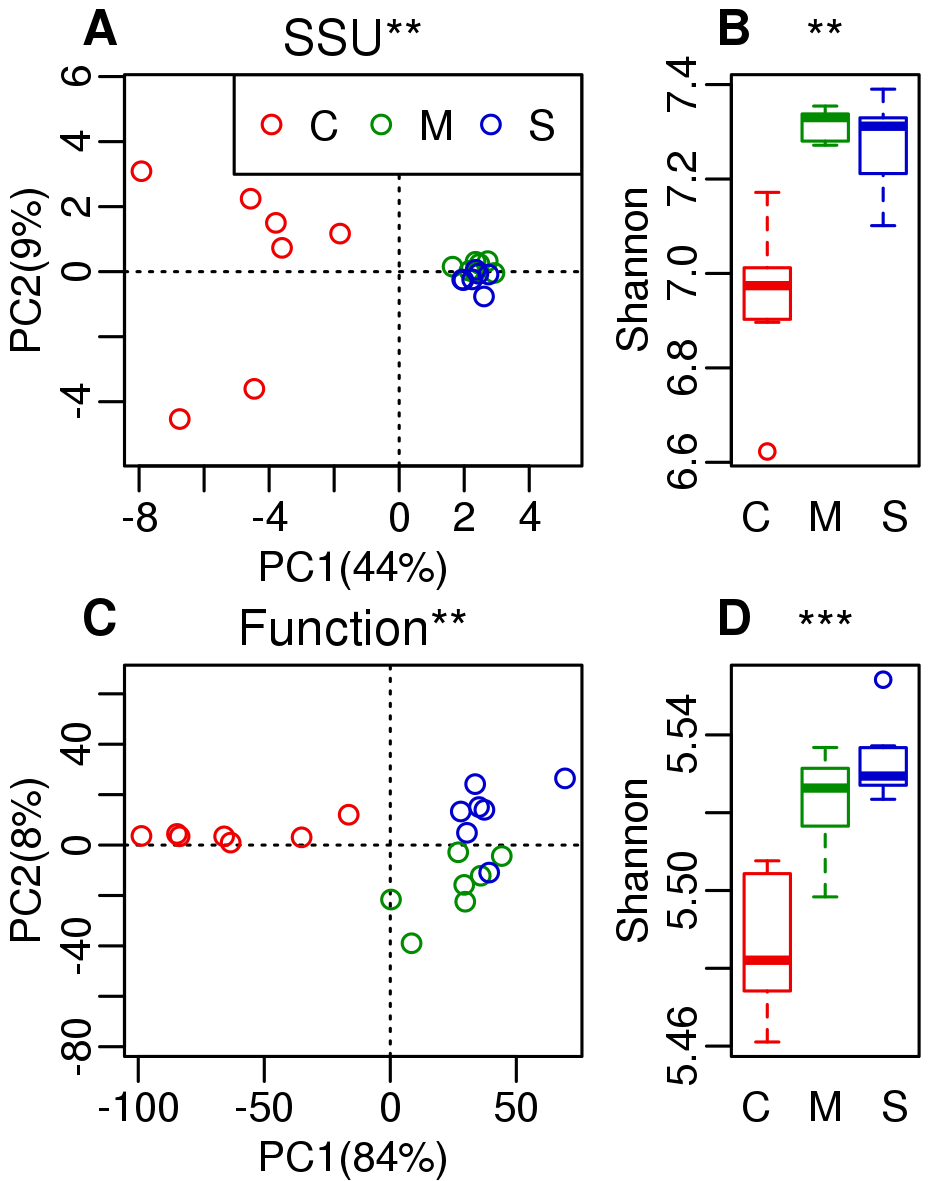
\includegraphics[scale=1]{figs/chap4-otu-subsys-pca-shannon}
  \caption[Species (OTU) and functional diversity comparsion among three crops]{Species (OTU) and functional diversity comparsion among three crops: C (corn), M (Miscanthus), and S (switchgrass) [These abbreviations are used throughout the paper]. Corn has a different community composition from Miscanthus and switchgrass in both OTU (A) and function (level 3 subsystems) (subplot C), and corn has lower diversity in both OTU (B) and function (D). The symbol at top each graph indicates significance of difference (``***'' indicates p < 0.001; ``**'' indicates p < 0.01; ``*'' indicates p < 0.05).}
  \label{fig:chap4Fig1}
\end{figure}


Microbial communities in perennials rhizosphere have higher species richness and diversity than corn rhizosphere in both alpha diversity (individual sample) and gamma diversity (samples merged by plant) (\cref{fig:chap4Fig1,fig:chap4FigS2}). Members in perennials are also more evenly distributed than in corn (\cref{fig:chap4FigS3}).

\begin{figure}[tbph!]
  \centering
  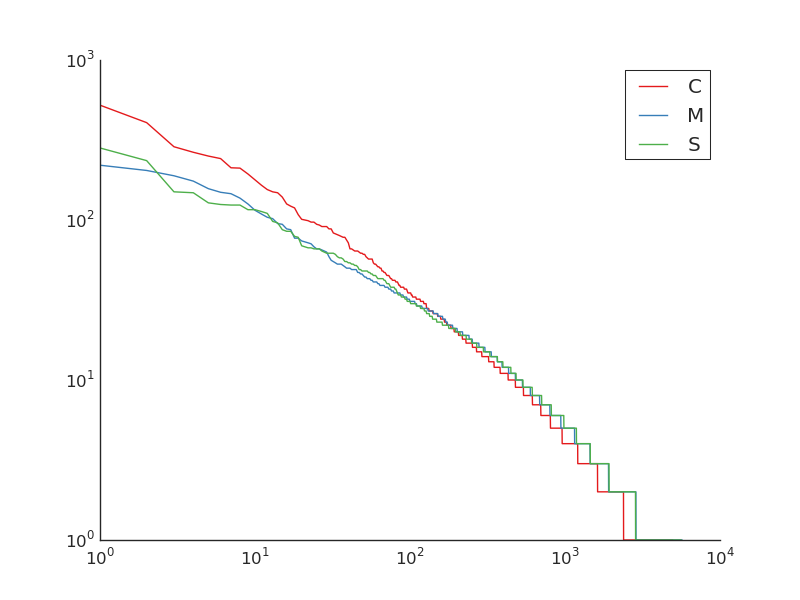
\includegraphics[scale=1]{figs/chap4-otu-rankabuncurve}
  \caption[Rank abundance curve of microbial communities in rhizosphere]{Rank abundance curve of microbial communities of corn (C), Miscanthus (M) and switchgrass (S) using OTU from SSU rRNA gene. Miscanthus and switchgrass have more even microbial community in rhizosphere than corn.}
  \label{fig:chap4FigS3}
\end{figure}



Corn had more proteobacteria in rhizosphere while perennials had more acidobacteria (\cref{fig:chap4Fig2}). Proteobacteria are mostly faster growers and Acidobacteria are mostly slow growers (41, 42)\cite{fierer_toward_2007,eilers_shifts_2010}. Thus corn selected for faster grower while perennials selected for slow growers. Top three genera are Sphingomonas (7.5\%, Proteobacteria), Penicillium (3.5\%, fungi), Burkholderia (3.4\%, Proteobacteria) in corn, Da023 (5.0\%, Acidobacteria), Akiw543 (4.1\%, Actinobacteria), Sphingomonas (3.1\%, Proteobacteria) in Miscanthus, and Da023 (6\%, Acidobacteria), Sphingomonas (4.0\%, Proteobacteria), and Akiw543 (3.2\%, Actinobacteria). Bacteria, Archaea, and Eukaryota were 91.9\%, 0.7\%, and 7.2\% respectively on average across all samples (Table \ref{tab:chap4TabS5}). Corn (4.9\%) had more fungi than Miscanthus (2.2\%) and switchgrass (2.0\%). However, relative abundance of AMF (Arbuscular Mycorrhizal Fungi) was lower in corn (0.1\%) than Miscanthus (0.3\%) and switchgrass (0.4\%).


\begin{figure}[tbph!]
  \centering
  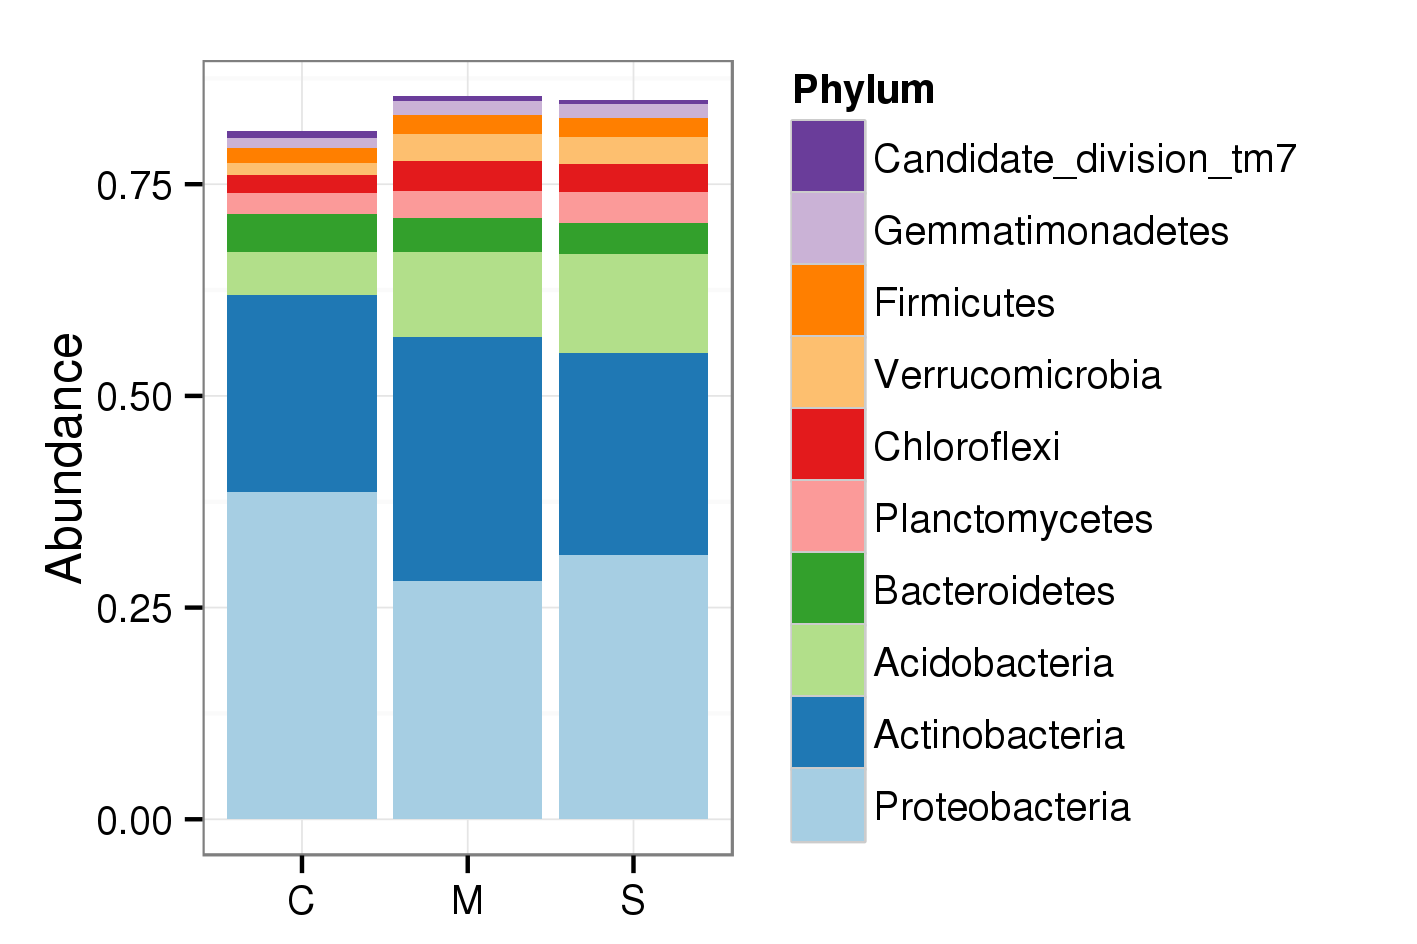
\includegraphics[scale=1]{figs/chap4-otu-bac-phylum}
  \caption[Relative abundance of top ten most abundant bacterial phyla in three crops]{Relative abundance of top ten most abundant bacterial phyla in three crops. Corn (C) is enriched in Proteobacteria (p < 0.01, n = 7), and Miscanthus (M) and switchgrass (S) are enriched in Acidobacteria (p < 0.001, n = 7). Average of Proteobacteria in corn, Miscanthus, and switchgrass are 0.387, 0.282, and 0.312 respectively. Average of Actinobacteria in corn, Miscanthus, and switchgrass are 0.050, 0.101, and 0.117 respectively. Average of Acidobacteria in corn, Miscanthus, and switchgrass are 0.050, 0.101, and 0.117 respectively.}
  \label{fig:chap4Fig2}
\end{figure}


\begin{table}[htbp]
  \centering
  \caption[Domain level distribution in rhizosphere communities]{Average percentage of Bacteria, Archaea, Eukaryota, and fungi in rhizosphere communities of corn (C), Miscanthus (M) and switchgrass (S).  “AMF/fungi” is percentage of AMF (arbuscular mycorrhizal  fungi) of total fungi.  Corn has more fungi in the whole community but has less percentage of AMF within fungi.}
    \begin{tabular}{|lrrrrr|}
    \toprule
          & Bac   & Arc   & Euk   & Fungi & AMF/fungi \\
    \midrule
    C     & 91.90\% & 0.70\% & 7.20\% & 4.90\% & 0.10\% \\
    M     & 94.10\% & 1.20\% & 4.50\% & 2.20\% & 0.30\% \\
    S     & 95.00\% & 0.90\% & 4.00\% & 2.00\% & 0.40\% \\
    \bottomrule
    \end{tabular}%
  \label{tab:chap4TabS5}%
\end{table}%




\textbf{Global assembly. }
We applied digital normalization and partitioning method \cite{howe_tackling_2014} to assemble pooled data (300 Gb) for each plant. The average computation time was 1510 CPU hours (63 days in total, Diginorm: 71h, Filterbelow: 25h, Loadgraph: 1166h, Partgraph: 205h, Mergegraph: 8h, Annograph: 27h, Extrgraph: 8h). Memory usage varied in difference steps. The peak memories used was 1 TB in digital normalization, which produced an average false positive rate of less than 0.01 in k-mer counting (false positive rates below 20\% were acceptable for digital normalization) \cite{zhang_these_2014}. Our assembly method produced assembly sizes ranged from 5.3 to 6.4 Gb with minimum contig size cutoff of 300 bp, and read mapping back rates (suggesting percentage of trimmed read data assembled) were similar among three crops (Table \ref{tab:chap4TabS4}). We also compared three crops based on sequence similarity among assemblies and found corn was the most different among three biofuel crops (Table \ref{tab:chap4TabS3}).

\begin{table}[htbp]
  \centering
  \caption[Global assembly statistics]{Global assembly statistics. Mapping\% is the percentage of reads mapped to contigs. C stands for corn, M stands for Miscanthus, and S stands for switchgrass.}
    \begin{tabular}{|lrrrrr|}
    \toprule
          & \multicolumn{1}{l}{Contig no. (M)} & \multicolumn{1}{l}{Total (Gbp)} & \multicolumn{1}{l}{Max (Kbp)} & \multicolumn{1}{l}{Median (bp)} & \multicolumn{1}{l|}{Mapping\%} \\
    \midrule
    C     & 12.9  & 6.4   & 21    & 400   & 20.7 \\
    M     & 12.9  & 6     & 15.7  & 391   & 19.1 \\
    S     & 11.4  & 5.3   & 16    & 391   & 20.3 \\
    \bottomrule
    \end{tabular}%
  \label{tab:chap4TabS4}%
\end{table}%


\textbf{Functional diversity using annotation from assembly. }
After the assembled sequences were annotated by MG-RAST, we used ``Subsystem'' annotation for further analysis. Ordination analysis with both subsystem level 1 and 3 showed corn was different perennials and no significant difference between Miscanthus and switchgrass (ADONIS: p < 0.01). The total variation explained crops were 74.7\% and 77.2\% at level 1 and 3 subsystems respectively (\cref{fig:chap4Fig1,fig:chap4FigS4}). The perennials significantly higher in functional diversity (Shannon) at both levels (p < 0.001, n = 7).

\begin{figure}[tbph!]
  \centering
  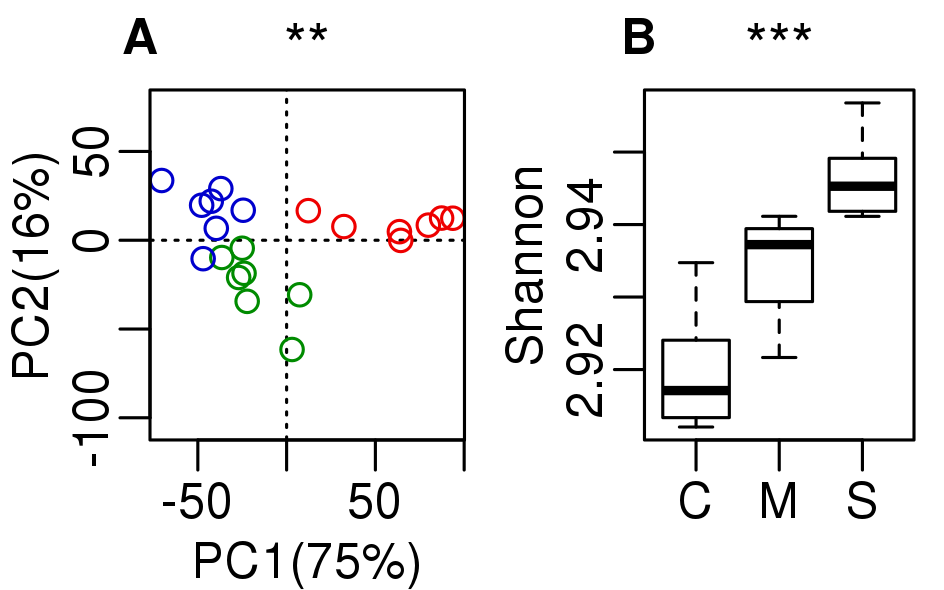
\includegraphics[scale=1]{figs/chap4-subsys-L1-pca-shannon}
  \caption[Functional diversity of three crops using subsystem level 1 ]{Functional diversity comparison among three crops. Corn has a different community functional composition from Miscanthus and switchgrass (level 1 subsystem) (A), and corn has lower diversity (B). C stands for corn, M stands for Miscanthus, and S stands for switchgrass. Symbols at top each subplot indicates significance of difference (``***'' indicates p < 0.001; ``**'' indicates p < 0.01; ``*'' indicates p < 0.05).}
  \label{fig:chap4FigS4}
\end{figure}


Since the above ordination analysis showed corn was the most different and perennials were similar, we picked Miscanthus as a representative of perennials and focus on the comparison between corn and Miscanthus. We focused on level 1 and level 3 subsystems for enrichment analysis since level 1 could give us overview of functions and level 3 could show pathway level information. Using level 1 subsystems, we found rhizosphere of corn was enriched in ``Iron acquisition and metabolism'', ``Membrane Transport'', ``Cell Wall and Capsule'', ``Phages, Prophages, Transposable elements, Plasmids'', ``Motility and Chemotaxis'', and ``Carbohydrate'', while Miscanthus was enriched in ``Amino Acids and Derivatives'', ``Cell Division and Cell Cycle'', ``Nucleosides and Nucleotides'', ``Protein Metabolism'', ``RNA Metabolism'', ``Secondary Metabolism'', ``Potassium metabolism'', ``Respiration'', ``Photosynthesis'', ``Regulation and Cell signaling'', and ``Stress Response'' (FDR adjusted p < 0.05, n = 7).

At level 3, we found corn had more pathways significantly enriched belonging to level 1 subsystems of ``Stress Response'', ``Carbohydrate'', and ``Cell Wall/Capsule'', while Miscanthus had more pathways significantly enriched in ``Amino Acids and Derivatives'', and ``Respiration'' (\cref{fig:chap4FigS5}). Within ``Stress response'', ``Desiccation stress'' and ``Oxidative stress'' were significantly higher in corn, while ``Cold shock'' and ``Osmotic stress'' were significantly higher in Miscanthus. Within “Carbohydrates”, “Sugar alcohols”, ``Aminosugars'', and ``Monosaccharides'' were enriched in corn, while ``CO2 fixation'', ``Central carbohydrate metabolism'', and ``Polysaccharides'' were enriched in Miscanthus. Within ``Phages, Prophages, Transposable elements, Plasmids'', ``Gene Transfer Agent (GTA)'', ``Plasmid related functions'', and ``Phages and prophages'' were enriched in corn, while ``Transposable elements'' were enriched in Miscanthus. Within ``Nitrogen Metabolism'', ``Nitrilase'' and ``Cyanate hydrosis'' were enriched in corn, while ``Dissimilatory nitrate reductase'', and ``Denitrification'', ``Allantoin Utilization'', ``Nitrogen Fixation'' were enriched in Miscanthus (FDR adjusted p < 0.05, n = 7).


\begin{figure}[tbph!]
  \centering
  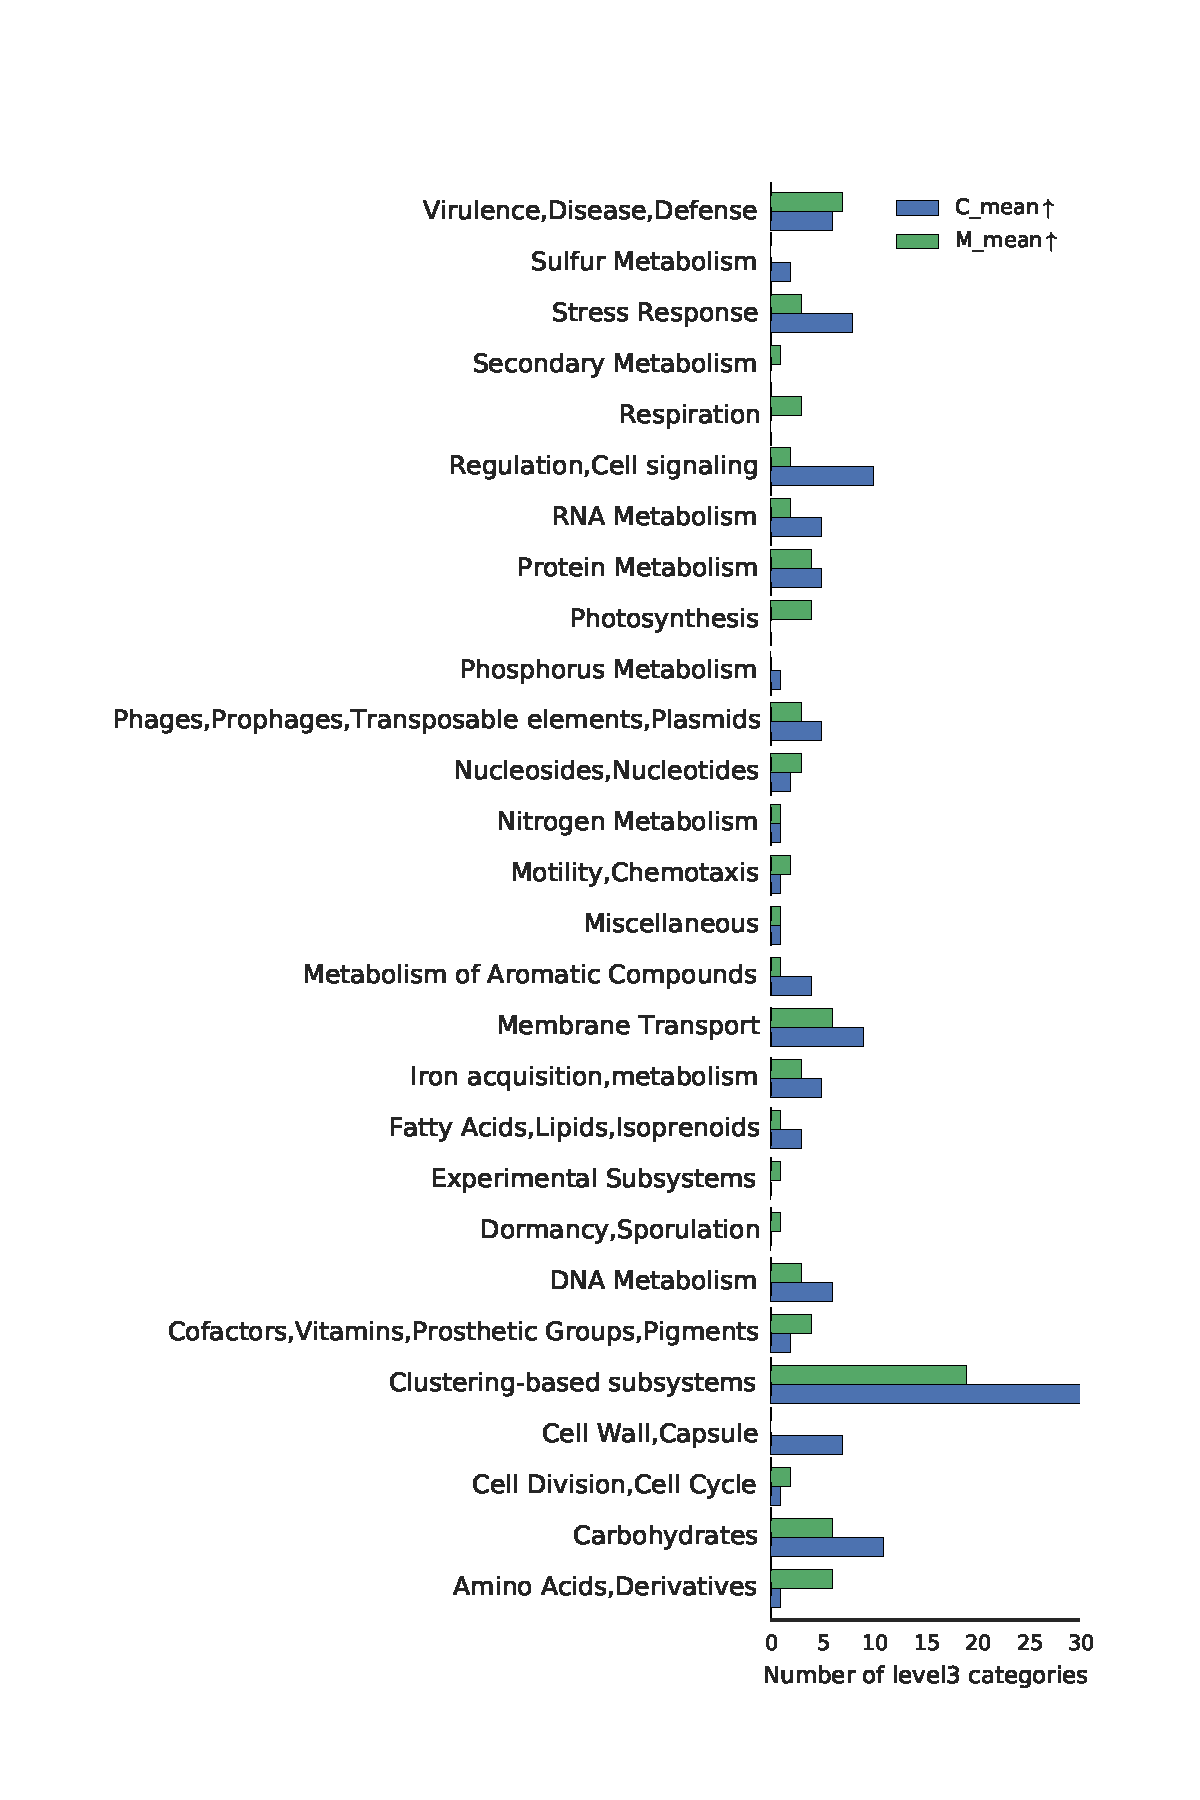
\includegraphics[width=0.60\textwidth]{figs/chap4-subsys-enrich-CvM}
  \caption[Function comparison between corn and Miscanthus]{Function comparison between corn and Miscanthus. Corn had more pathways significantly enriched belonging to level 1 subsystems of ``Stress Response'', ``Carbohydrate'', and ``Cell Wall/Capsule'', while Miscanthus had more pathways significantly enriched in ``Amino Acids and Derivatives'', and ``Respiration''. Signifcance of enrichment is done by Kruskal-Wallis test. Those level 3 pathways with FDR (False Discovery Rate) adjust p < 0.05, total count larger than 10 and ratio of corn over Miscanthus (in log2 space) larger than 1.5  or smaller than -1.5 are chosen as significant.}
  \label{fig:chap4FigS5}
\end{figure}



\textbf{N cycle gene diversity. }
All the N cycle genes except AOA showed those subgroups were significantly different among three crops (\cref{fig:chap4Fig3}). In terms of richness and diversity, nosZ, nosZa2, cNor, and qNor showed significant difference among three crops (\cref{fig:chap4FigS6,fig:chap4FigS7}. For the above four genes, Miscanthus and switchgrass were both significantly higher than corn (p < 0.05, n = 7).


\begin{figure}[tbph!]
  \centering
  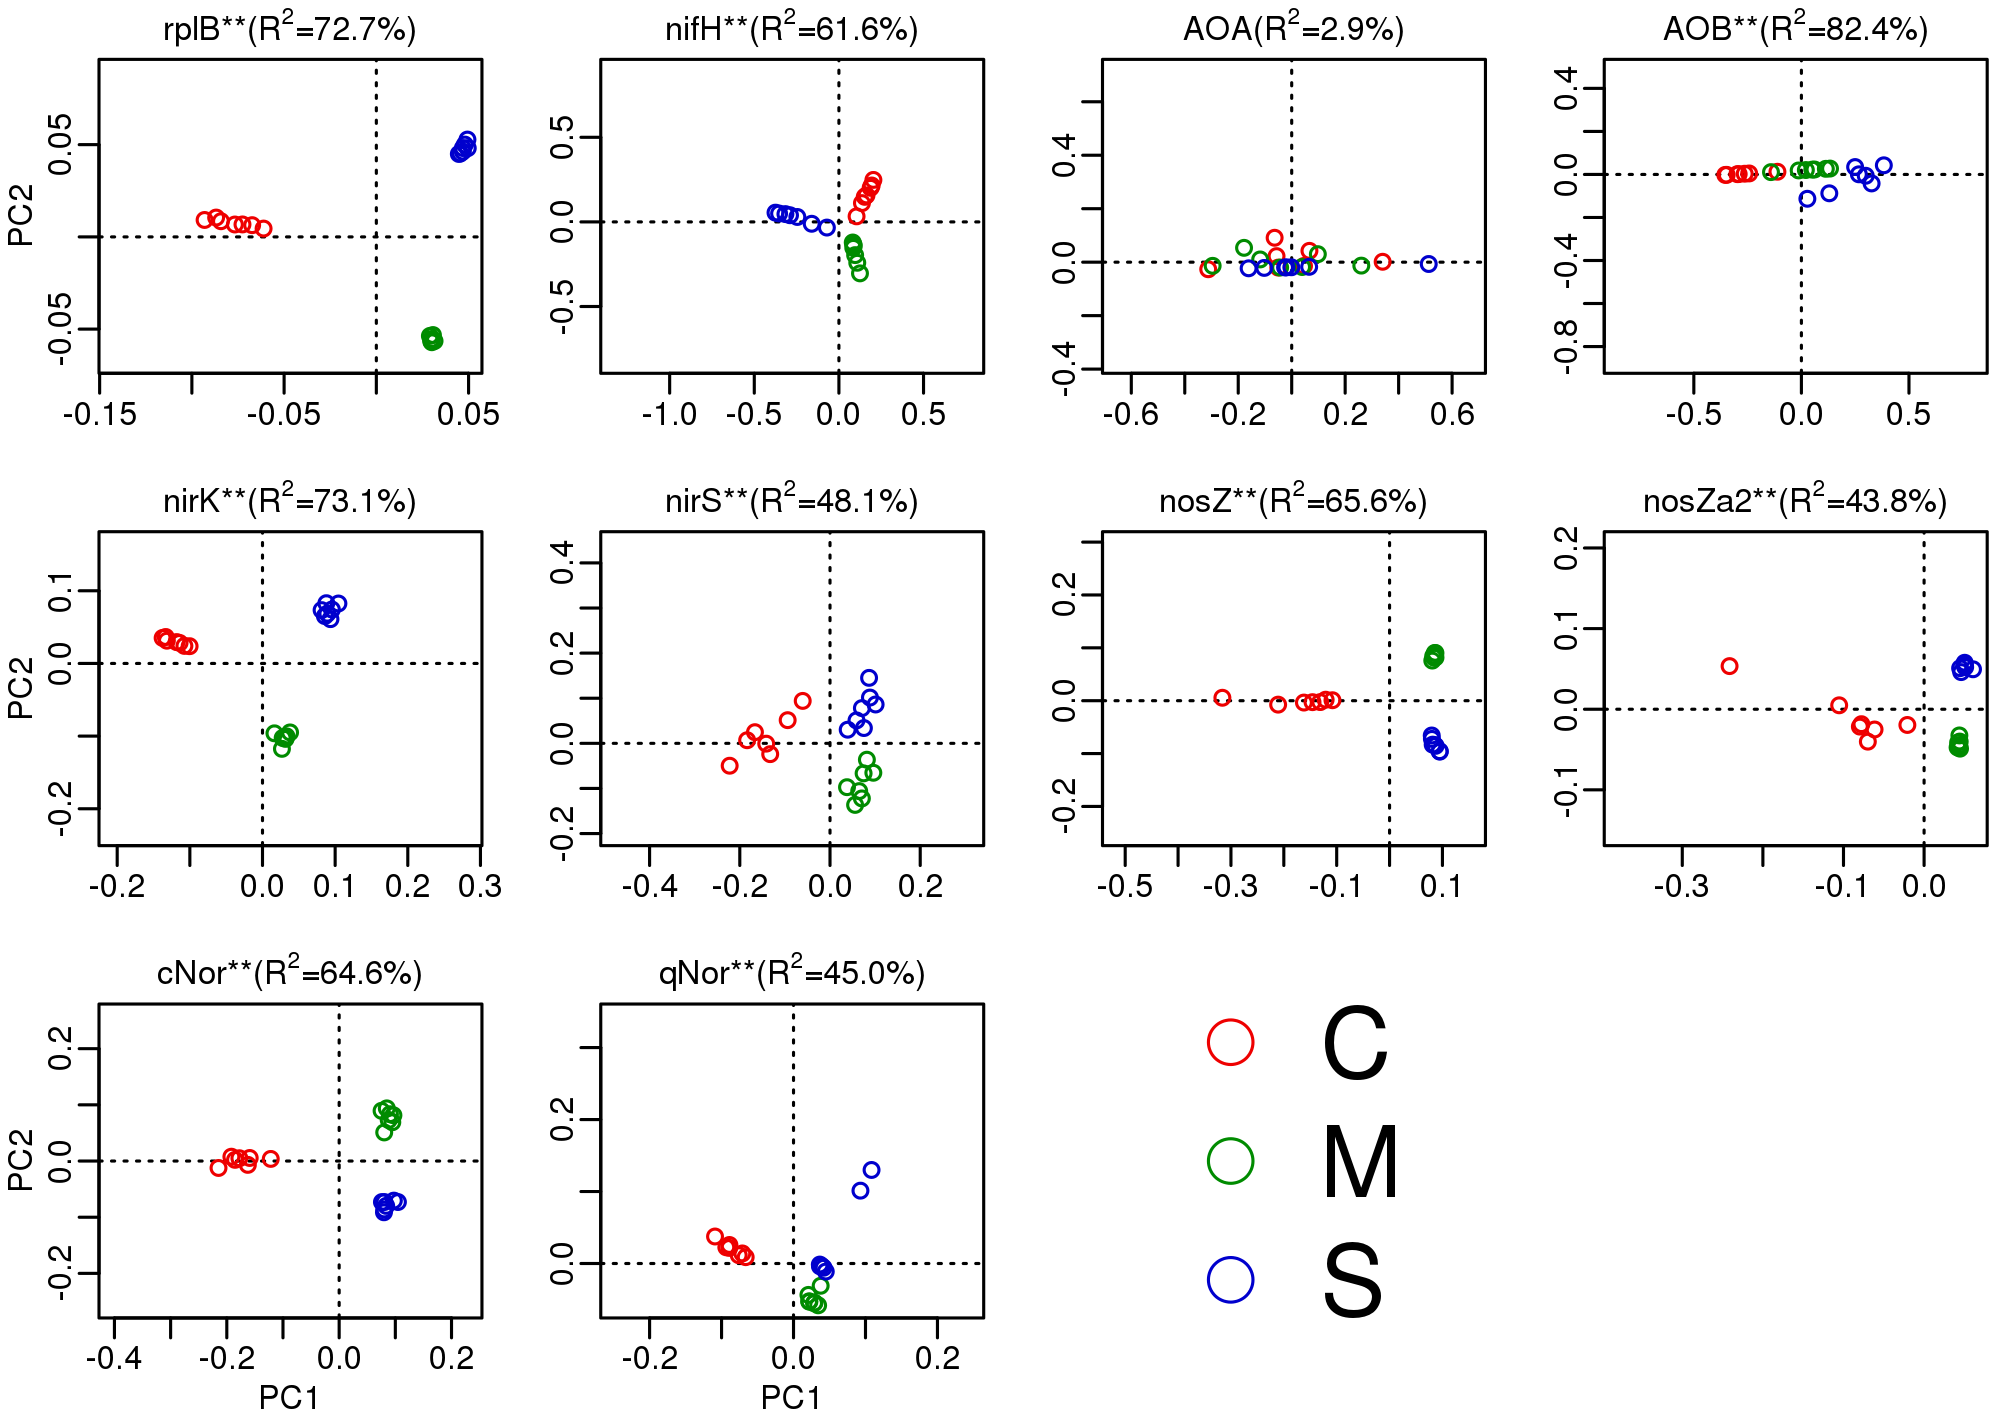
\includegraphics[scale=1]{figs/chap4-xander-ncycle-otu-pca}
  \caption[Ordination analysis of each N cycle gene and rplB using OTU]{Ordination analysis of each N cycle gene and rplB using OTU. All genes except AOA show significant separation of samples by corn (C), Miscanthus (M) and switchgrass (S). OTUs of each gene are clustered at 5\% distance cutoff using protein sequence.}
  \label{fig:chap4Fig3}
\end{figure}


\begin{figure}[tbph!]
  \centering
  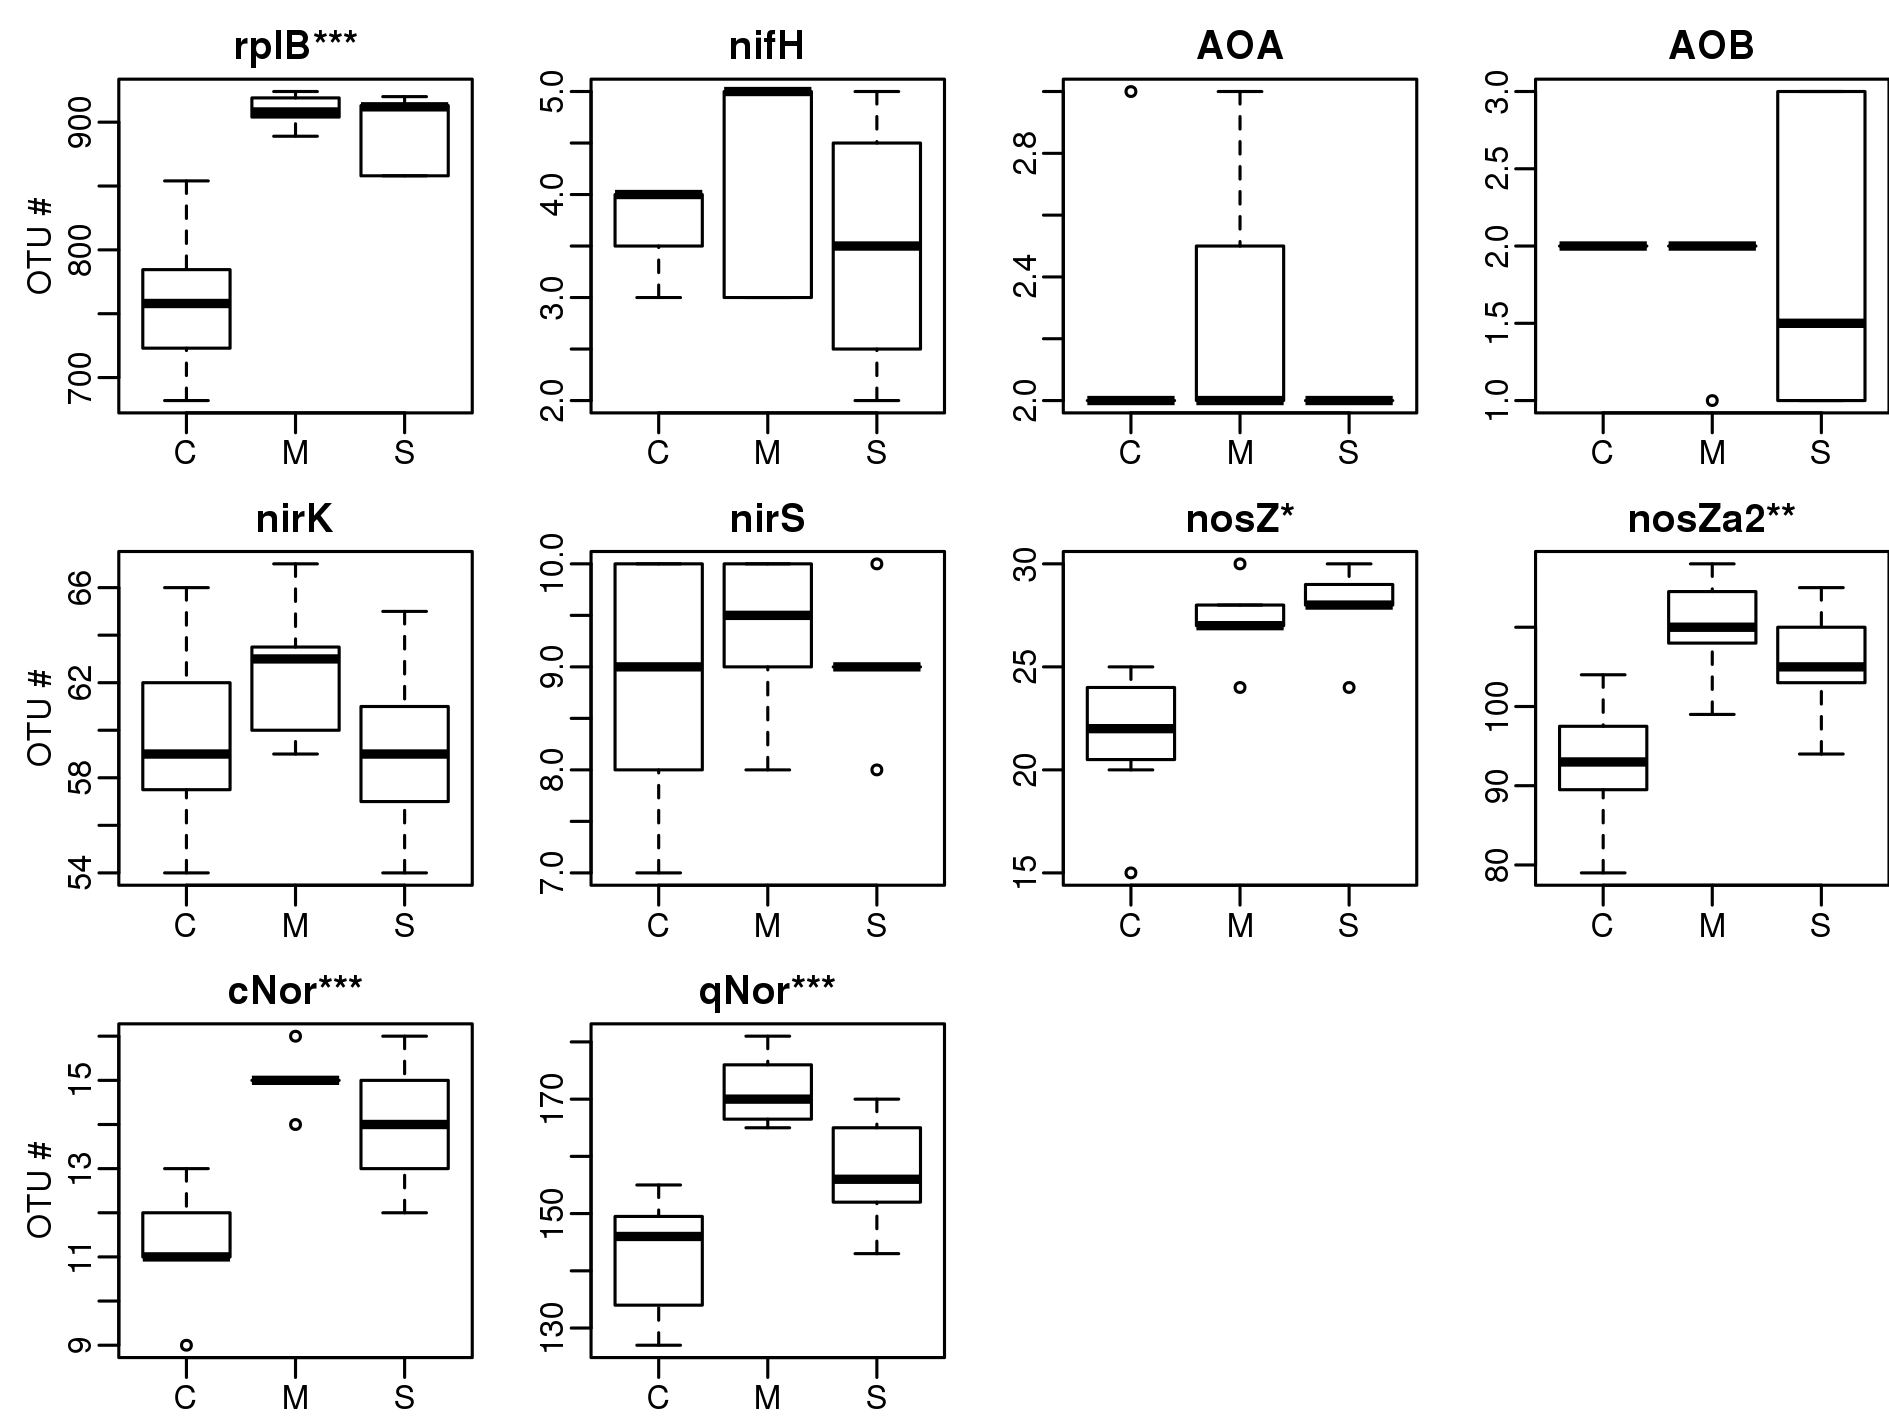
\includegraphics[scale=1]{figs/chap4-xander-ncycle-otu-count}
  \caption[N cycle gene OTU number comparison among three crops]{OTU number comparison among corn (C), Miscanthus (M) and switchgrass (S) using OTU tables of N cycle genes. Y axis of each plot shows OTU number. Symbols at top each subplot indicate significance of difference (``***'' indicates p < 0.001; ``**'' indicates p < 0.01; ``*'' indicates p < 0.05, ``.'' indicates p<0.1).}
  \label{fig:chap4FigS6}
\end{figure}


\begin{figure}[tbph!]
  \centering
  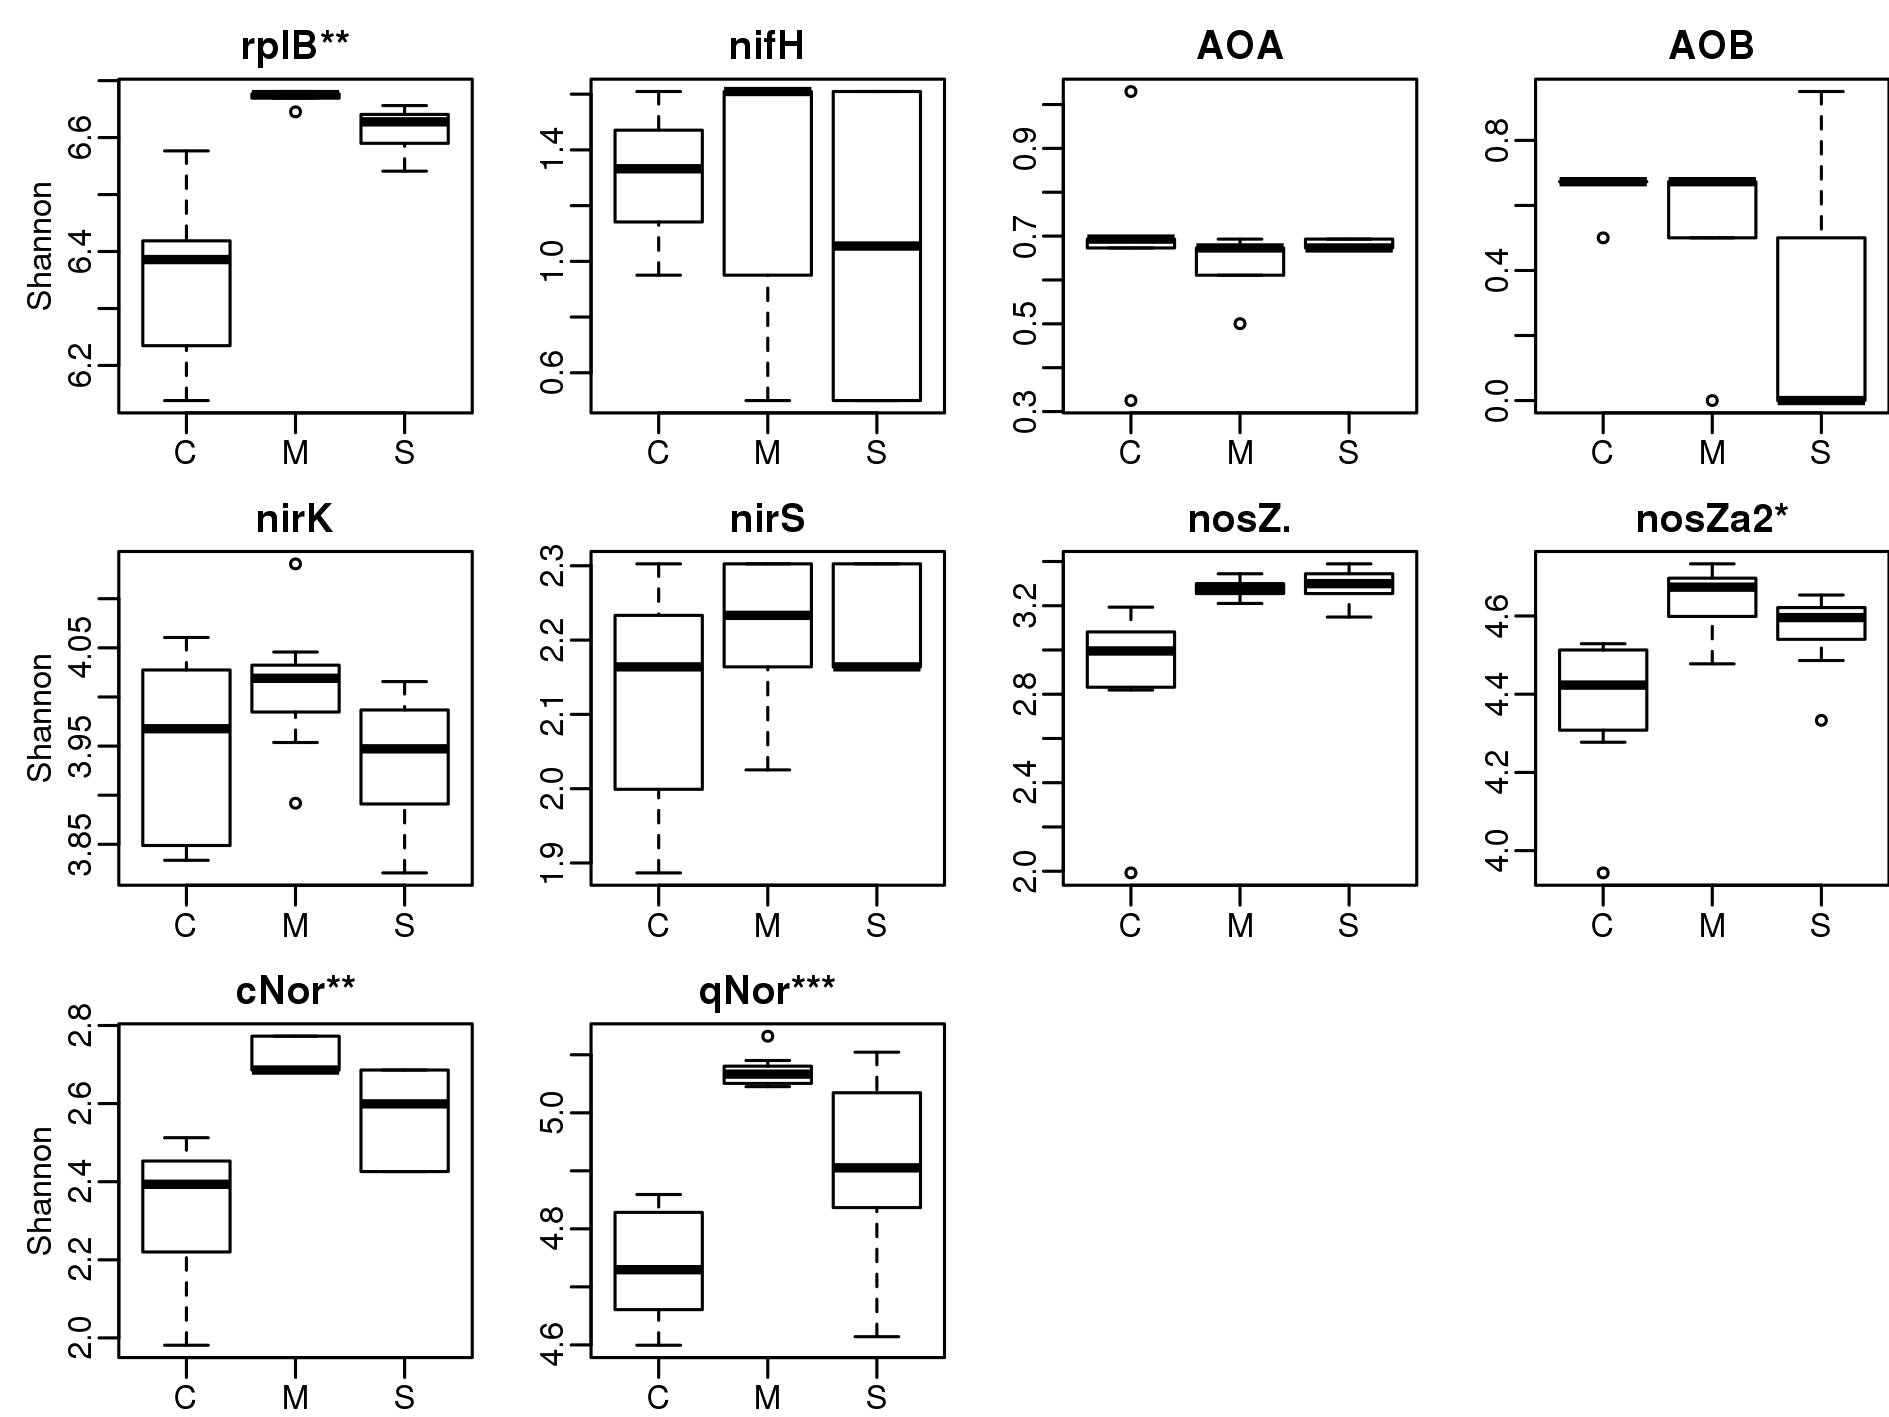
\includegraphics[scale=1]{figs/chap4-xander-ncycle-otu-shannon}
  \caption[N cycle gene diversity of three crops]{Diversity (Shannon) comparison among corn (C), Miscanthus (M) and switchgrass (S) using OTU tables of N cycle genes. Symbols at top each subplot indicate significance of difference (``***'' indicates p < 0.001; ``**'' indicates p < 0.01; ``*'' indicates p < 0.05, ``.'' indicates p<0.1).}
  \label{fig:chap4FigS7}
\end{figure}


\textbf{N cycle gene abundance and taxonomy composition. }
We used Xander \cite{wang_xander:_2015}, a gene targeted assembler, to assemble the N cycle genes for further diversity analysis of this functionally important group. \Cref{fig:chap4Fig4} showed N cycle genes abundances, including nitrogen fixation genes (nifH), nitrification genes (AOA and AOB), and denitrification genes (nirK, nirS, nosZ, nosZa2, qNor, and cNor) normalized by rplB abundance. NifH, AOB, nirK, nosZa2, and qNor were significantly different between corn and Miscanthus. NirK, nosZ and qNor were significantly different between corn and switchgrass. AOA and nosZ was significantly different between Miscanthus and switchgrass (p < 0.05, n = 7).

When combining the genes coding enzymes with the same function, nitrite reductase genes (nirK and nirS) are significantly more abundant in corn, but nitric oxide reductase genes (qNor and cNor) and nitrous oxide reductase genes (nosZ and nosZa2) are significantly more abundant in perennials (\cref{fig:chap4Fig5}). Further, we looked at the ratio of nitrification/fixation (amoA/nifH) and denitrification/nitrification ((nirK+nirS)/amoA, (qNor+cNor)/amoA, and (nosZ+nosZa2)/amoA). Differences among three crops of all the above ratios were not significant at $\alpha = 0.05$ level. However, median of amoA/nifH is the highest in corn and median of (nirK+nirS)/amoA, (cNor+qNor)/amoA, and (nosZ+nosZa2)/amoA are all highest in switchgrass (\cref{fig:chap4FigS8}).



\begin{figure}[tbph!]
  \centering
  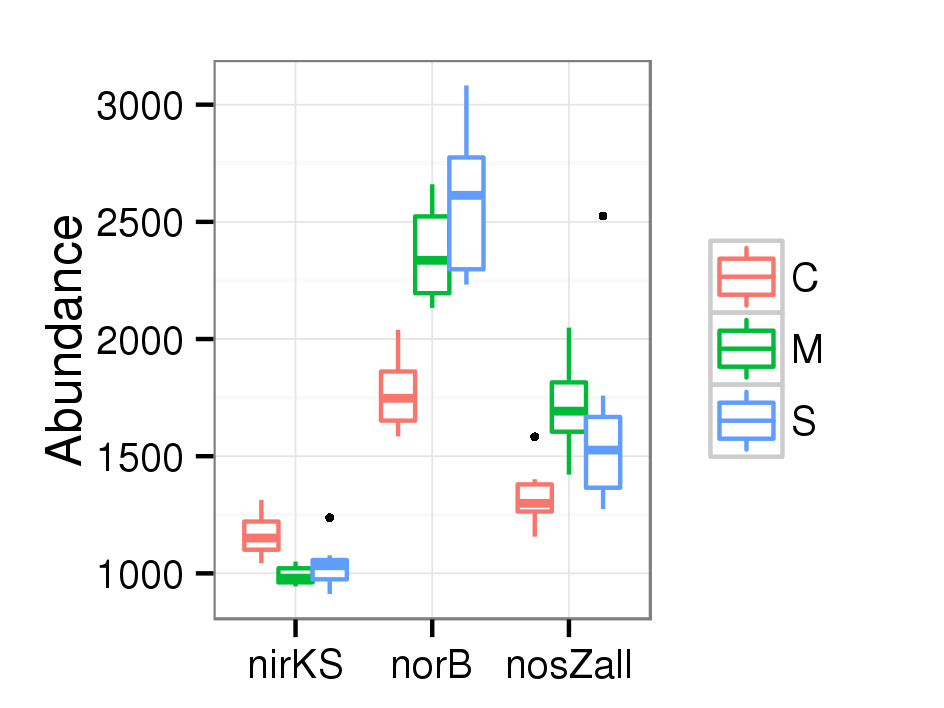
\includegraphics[scale=1]{figs/chap4-xander-denitrify-abun-merge-pair}
  \caption[]{Denitrification gene abundances after combining the genes encoding enzymes with the same function. ``NirKS'' = nirK and nirS. ``NorB'' = cNor and qNor. ``NosZall'' = nosZ and nosZa2. Each gene’s abundance is normalized relative to rplB copies. Three crops are significantly different in abundances of “nirKS”, ``norB'', and ``nosZall'' (p < 0.05, n = 7). Corn is higher than perennials in abundance of ``nirKS'' but lower in abundance of ``norB'' and ``nosZall''.}
  \label{fig:chap4Fig5}
\end{figure}


\begin{figure}[tbph!]
  \centering
  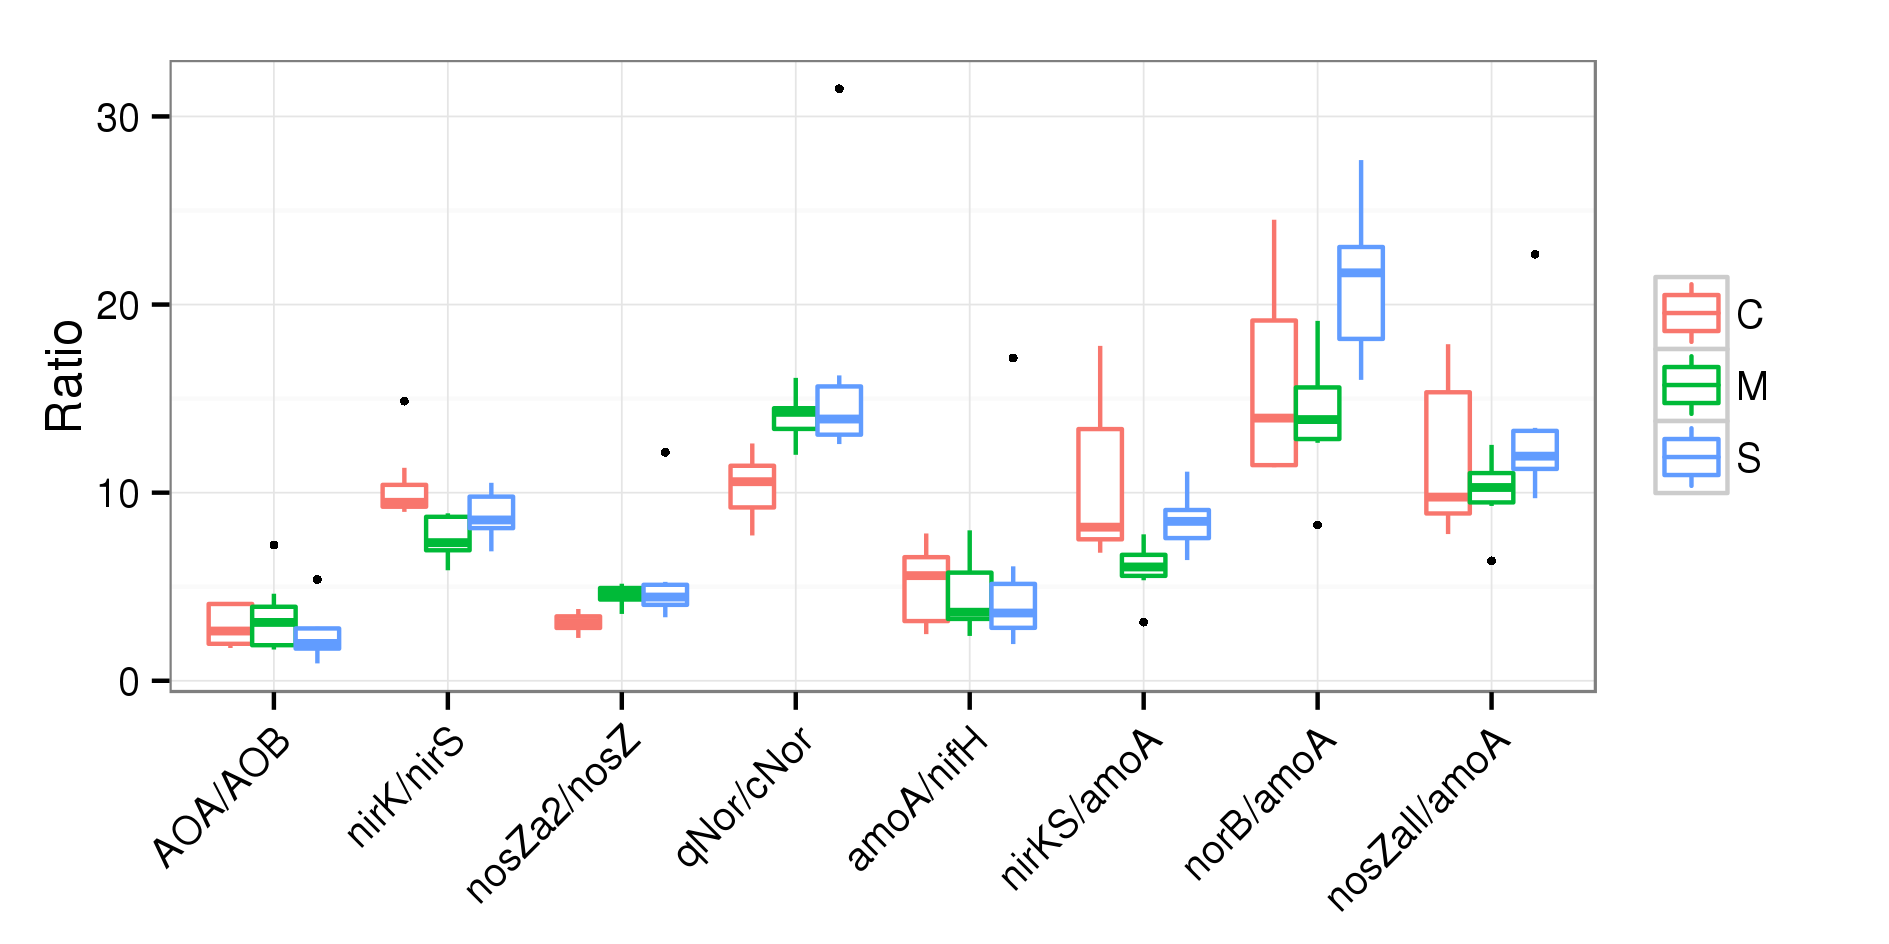
\includegraphics[scale=1]{figs/chap4-xander-ncycle-ratio}
  \caption[Ratios of interest related to N cycle genes]{Ratios of interest related to N cycle genes in corn (C), Miscanthus (M) and switchgrass (S). ``AmoA'' is the sum of AOA and AOB; ``nirKS'' is the sum of nirK and nirS; ``norB'' is the sum of cNor and qNor; ``nosZall'' is the sum of nosZ and nosZa2. Each ratio is grouped by plant (7 replicates).}
  \label{fig:chap4FigS8}
\end{figure}



We also found a consistent pattern across all samples for those gene pairs coding enzymes with same function: AOA > AOB, nirK > nirS, nosZa2 > nosZ, qNor > cNor (\cref{fig:chap4Fig4,fig:chap4FigS8}). Moreover, nitrification gene abundances (AOA and AOB) were higher than nitrogen fixation genes (nifH), and denitrification gene abundances (nirK and nirS, qNor and cNor, or nosZ and nosZa2) were higher than nitrification genes (AOA and AOB) (\cref{fig:chap4Fig4,fig:chap4FigS8}).


\begin{figure}[tbph!]
  \centering
  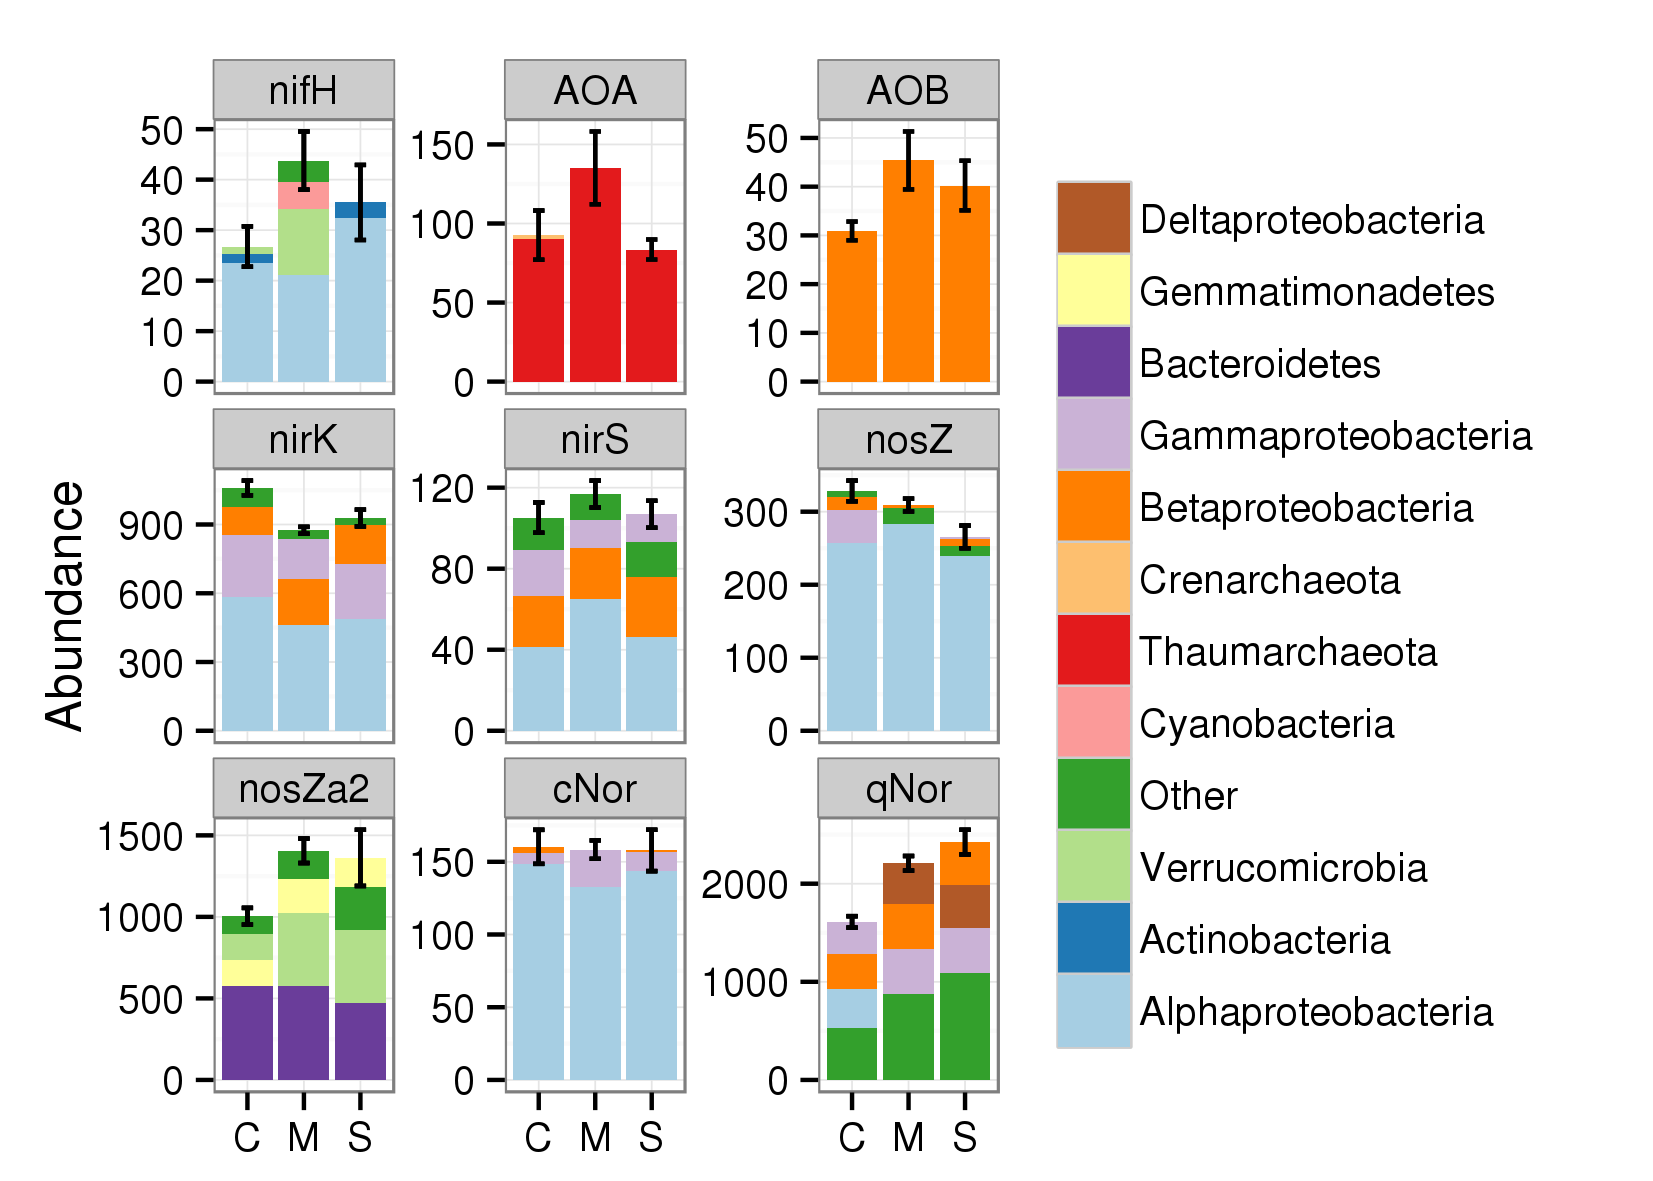
\includegraphics[scale=1]{figs/chap4-xander-ncycle-abun}
  \caption[Abundance and phylum association of the indicated N cycle genes]{Abundance and phylum level association of the indicated N cycle genes in corn (C), Miscanthus (M) and switchgrass (S). Gene abundances are normalized relative to rplB copies. There are significant differences among three crops in nirK, nosZ, nosZa2 and qNor (p < 0.05, n = 7). Additionally, pairwise t test shows Miscanthus is significantly higher than corn in nifH and AOB (p < 0.05, n = 7).}
  \label{fig:chap4Fig4}
\end{figure}


We then looked at detailed genus level distribution of nifH. There were 7, 9, and 5 genera in corn, Miscanthus, and switchgrass, respectively (\cref{fig:chap4Fig6}). The taxonomic compositions of the communities were different among three crops. On average, \textit{Rhizobium}, \textit{Bradyrhizobium}, and \textit{Methylobacterium} were the most abundant in corn, \textit{Coraliomargarita}, \textit{Azospirillum}, and Nostoc were the most abundant in Miscanthus, and \textit{Novosphigobium}, \textit{Gluconacetobacter}, and \textit{Azospirillum} were the most abundant in switchgrass (\cref{fig:chap4Fig6}).


\begin{figure}[tbph!]
  \centering
  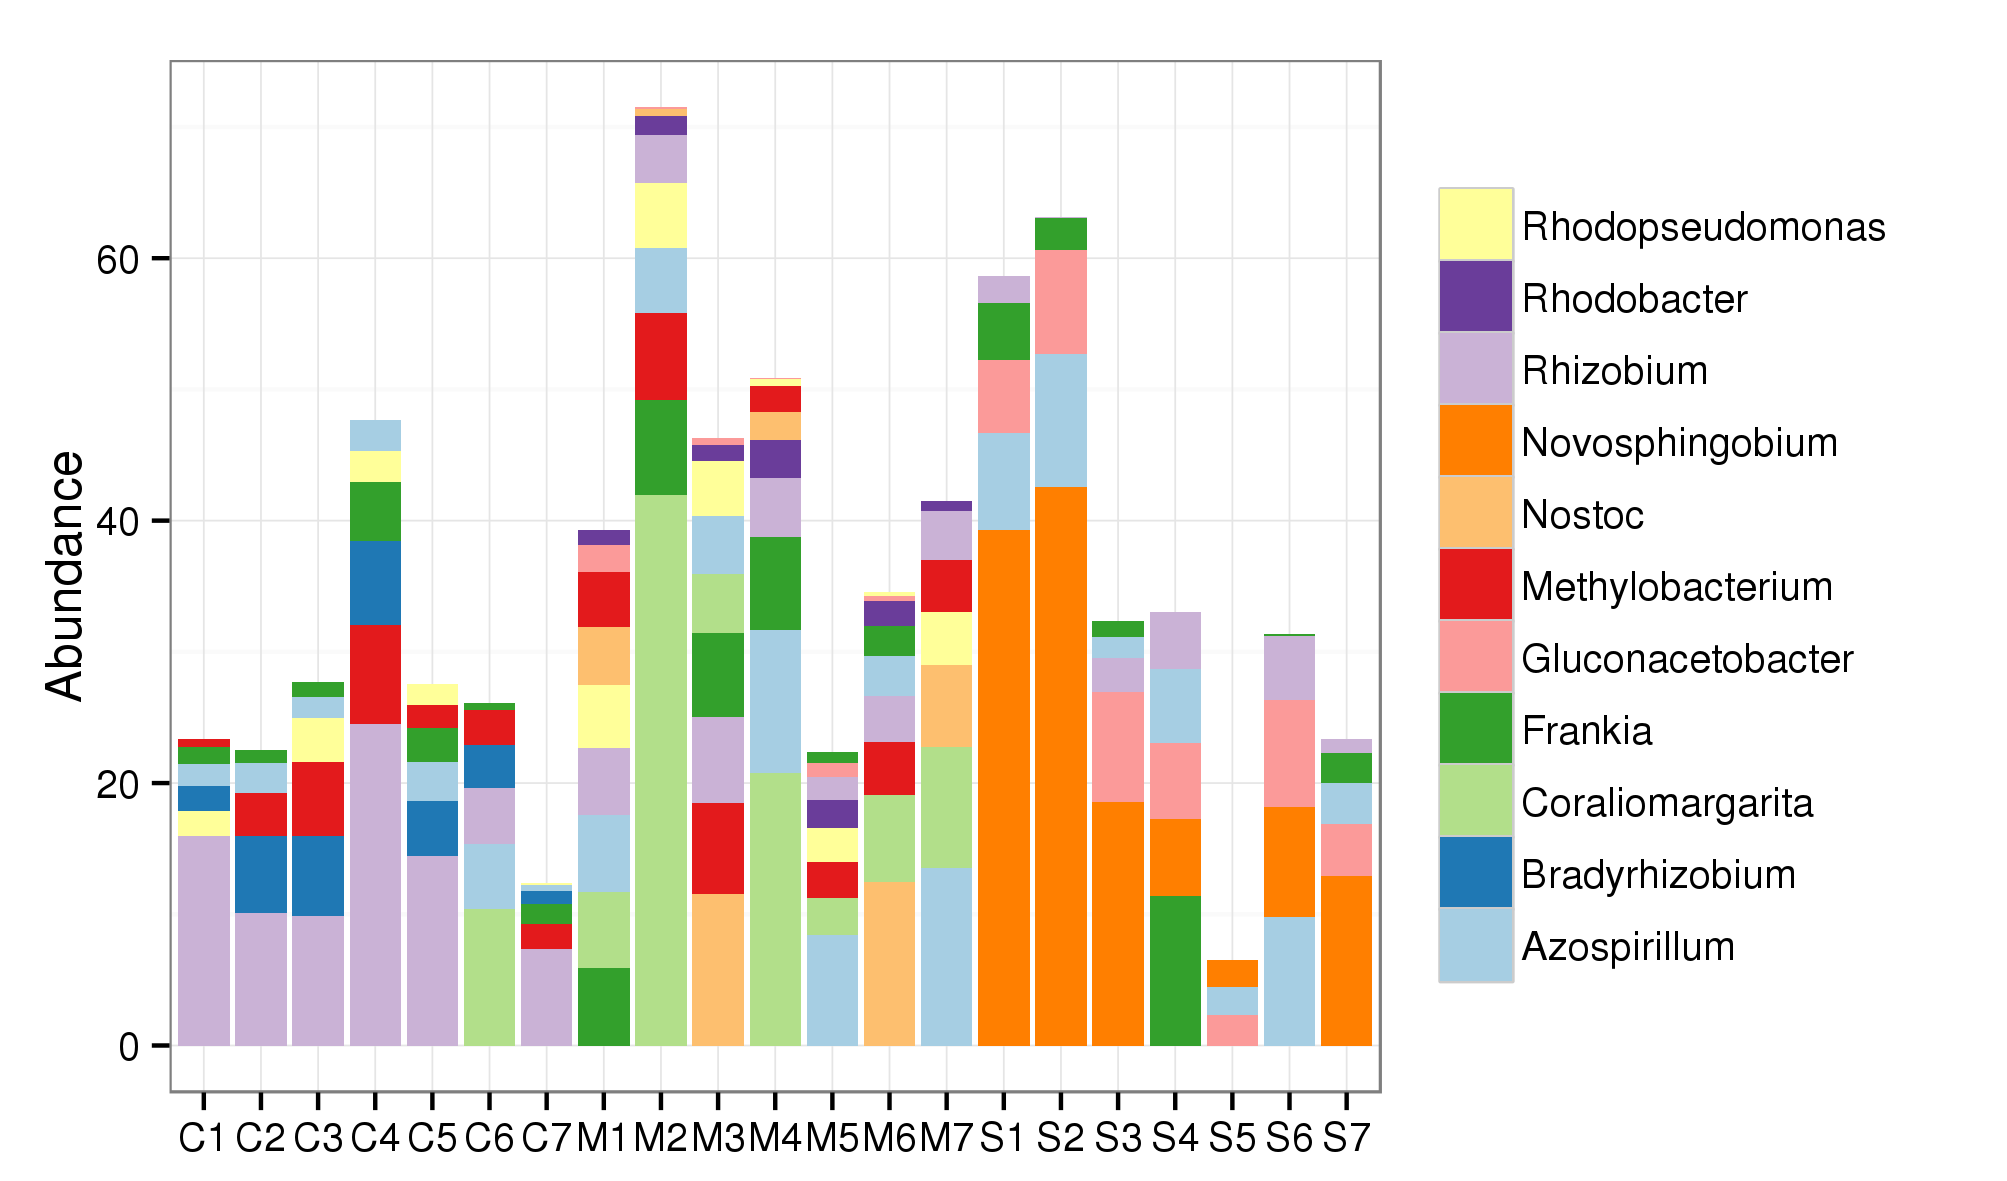
\includegraphics[scale=1]{figs/chap4-xander-nifH-genus-rep}
  \caption[Abundance and genus level distribution of nifH]{Abundance and genus level distribution of nifH. Y axis is gene abundance normalized relative to rplB copies. X axis is sample labels in which first letter stands for crop (C for corn, M for Miscanthus, and S for switchgrass). Three crops rhizospheres are quite different in genera with the closest sequence match. On average, \textit{Rhizobium}, \textit{Bradyrhizobium}, and \textit{Methylobacterium}-like sequences are the most abundant in corn, \textit{Coraliomargarita}, \textit{Azospirillum}, and Nostoc the most abundant in Miscanthus, and \textit{Novosphigobium}, \textit{Gluconacetobacter}, and \textit{Azospirillum} the most abundant in switchgrass.}
  \label{fig:chap4Fig6}
\end{figure}


Since Xander assigned the taxonomy based on best hit to reference sequences, some assembled sequences might be quite different from its best-hit reference sequence and thus distant from its assigned taxon. Thus we examined the similarity distribution of our assembled sequences to references. Identities of assembled sequence to references range from 79.3\% to 100\% for nifH, 93.5\% to 97.5\% for AOA, 95.6\% to 98.9\% for AOB, 58.5\% to 97.3\% for nirK, 68.5\% to 94.8\% for nirS, 65.7\% to 99.2\% for nosZ, 54.7\% to 97.7\% for nosZa2, 71.1\% to 98.4\% for cNor, and 51.9\% to 98.3\% for qNor (\cref{fig:chap4FigS9}). For nifH, the most abundant genera in corn, Miscanthus, and switchgrass has assembled sequences with lowest identity of 89.5\% (\textit{Rhizobium}), 83.1\% (\textit{Coraliomargarita}), 92.4\% (\textit{Novosphingobium}), respectively (\cref{fig:chap4FigS10}).

\begin{figure}[tbph!]
  \centering
  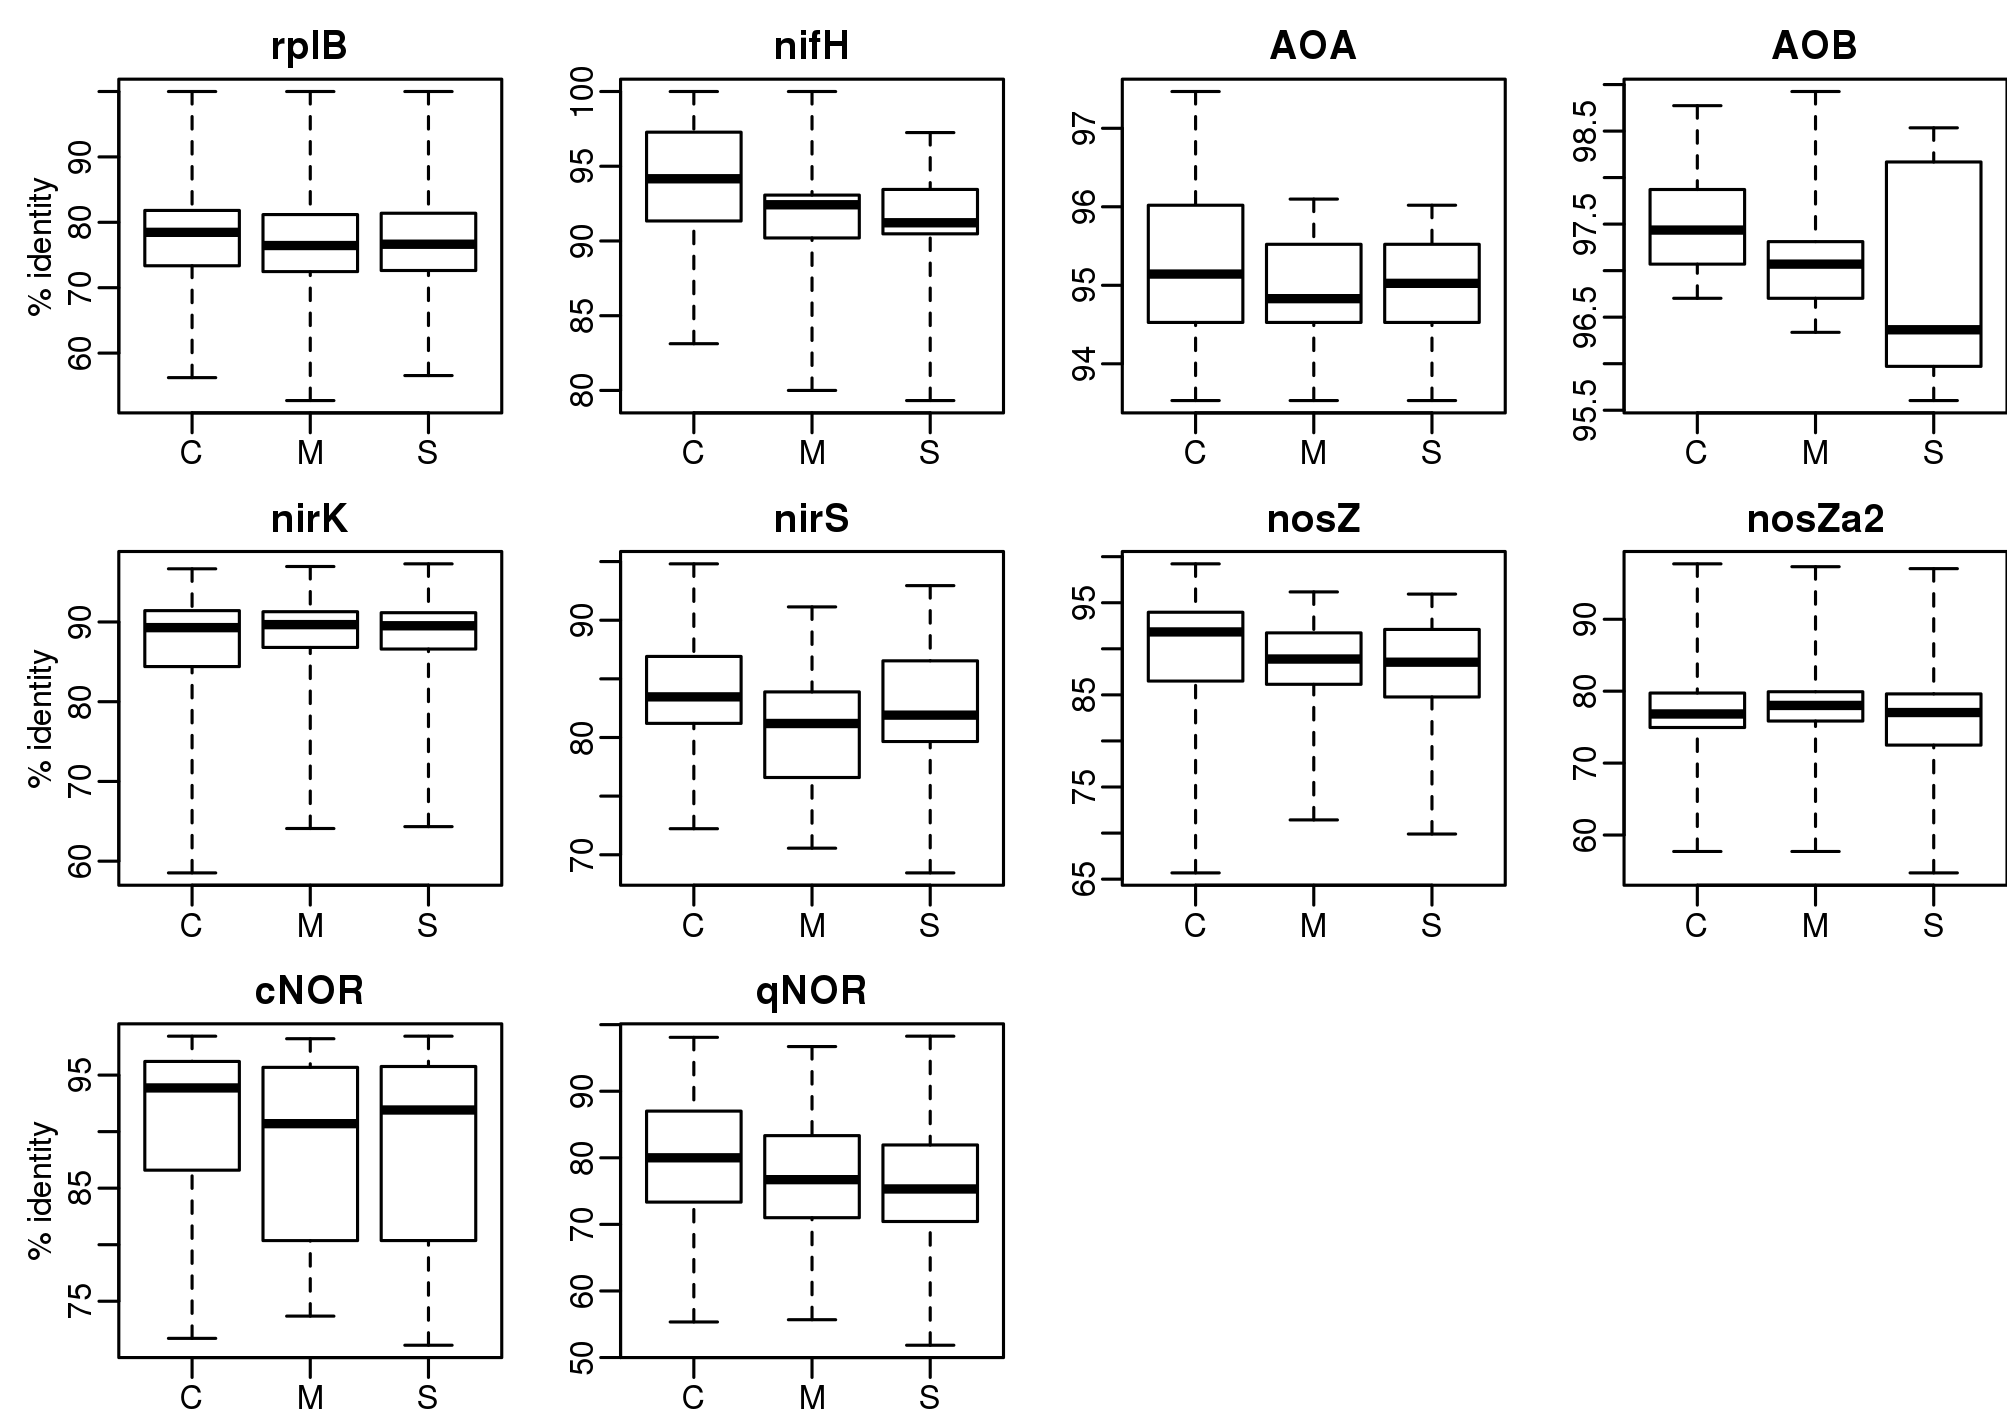
\includegraphics[scale=1]{figs/chap4-xander-ncycle-similarity}
  \caption[Identity of assembled N cycle genes to their best-hit references]{Sequence identity of assembled N cycle genes to their best-hit references. Percentage identities (Y axis) are grouped by plant (C for corn, M for Miscanthus, and S for switchgrass). The lower identiy is, the more likely a assembled sequence is in correctly classified.}
  \label{fig:chap4FigS9}
\end{figure}


\begin{figure}[tbph!]
  \centering
  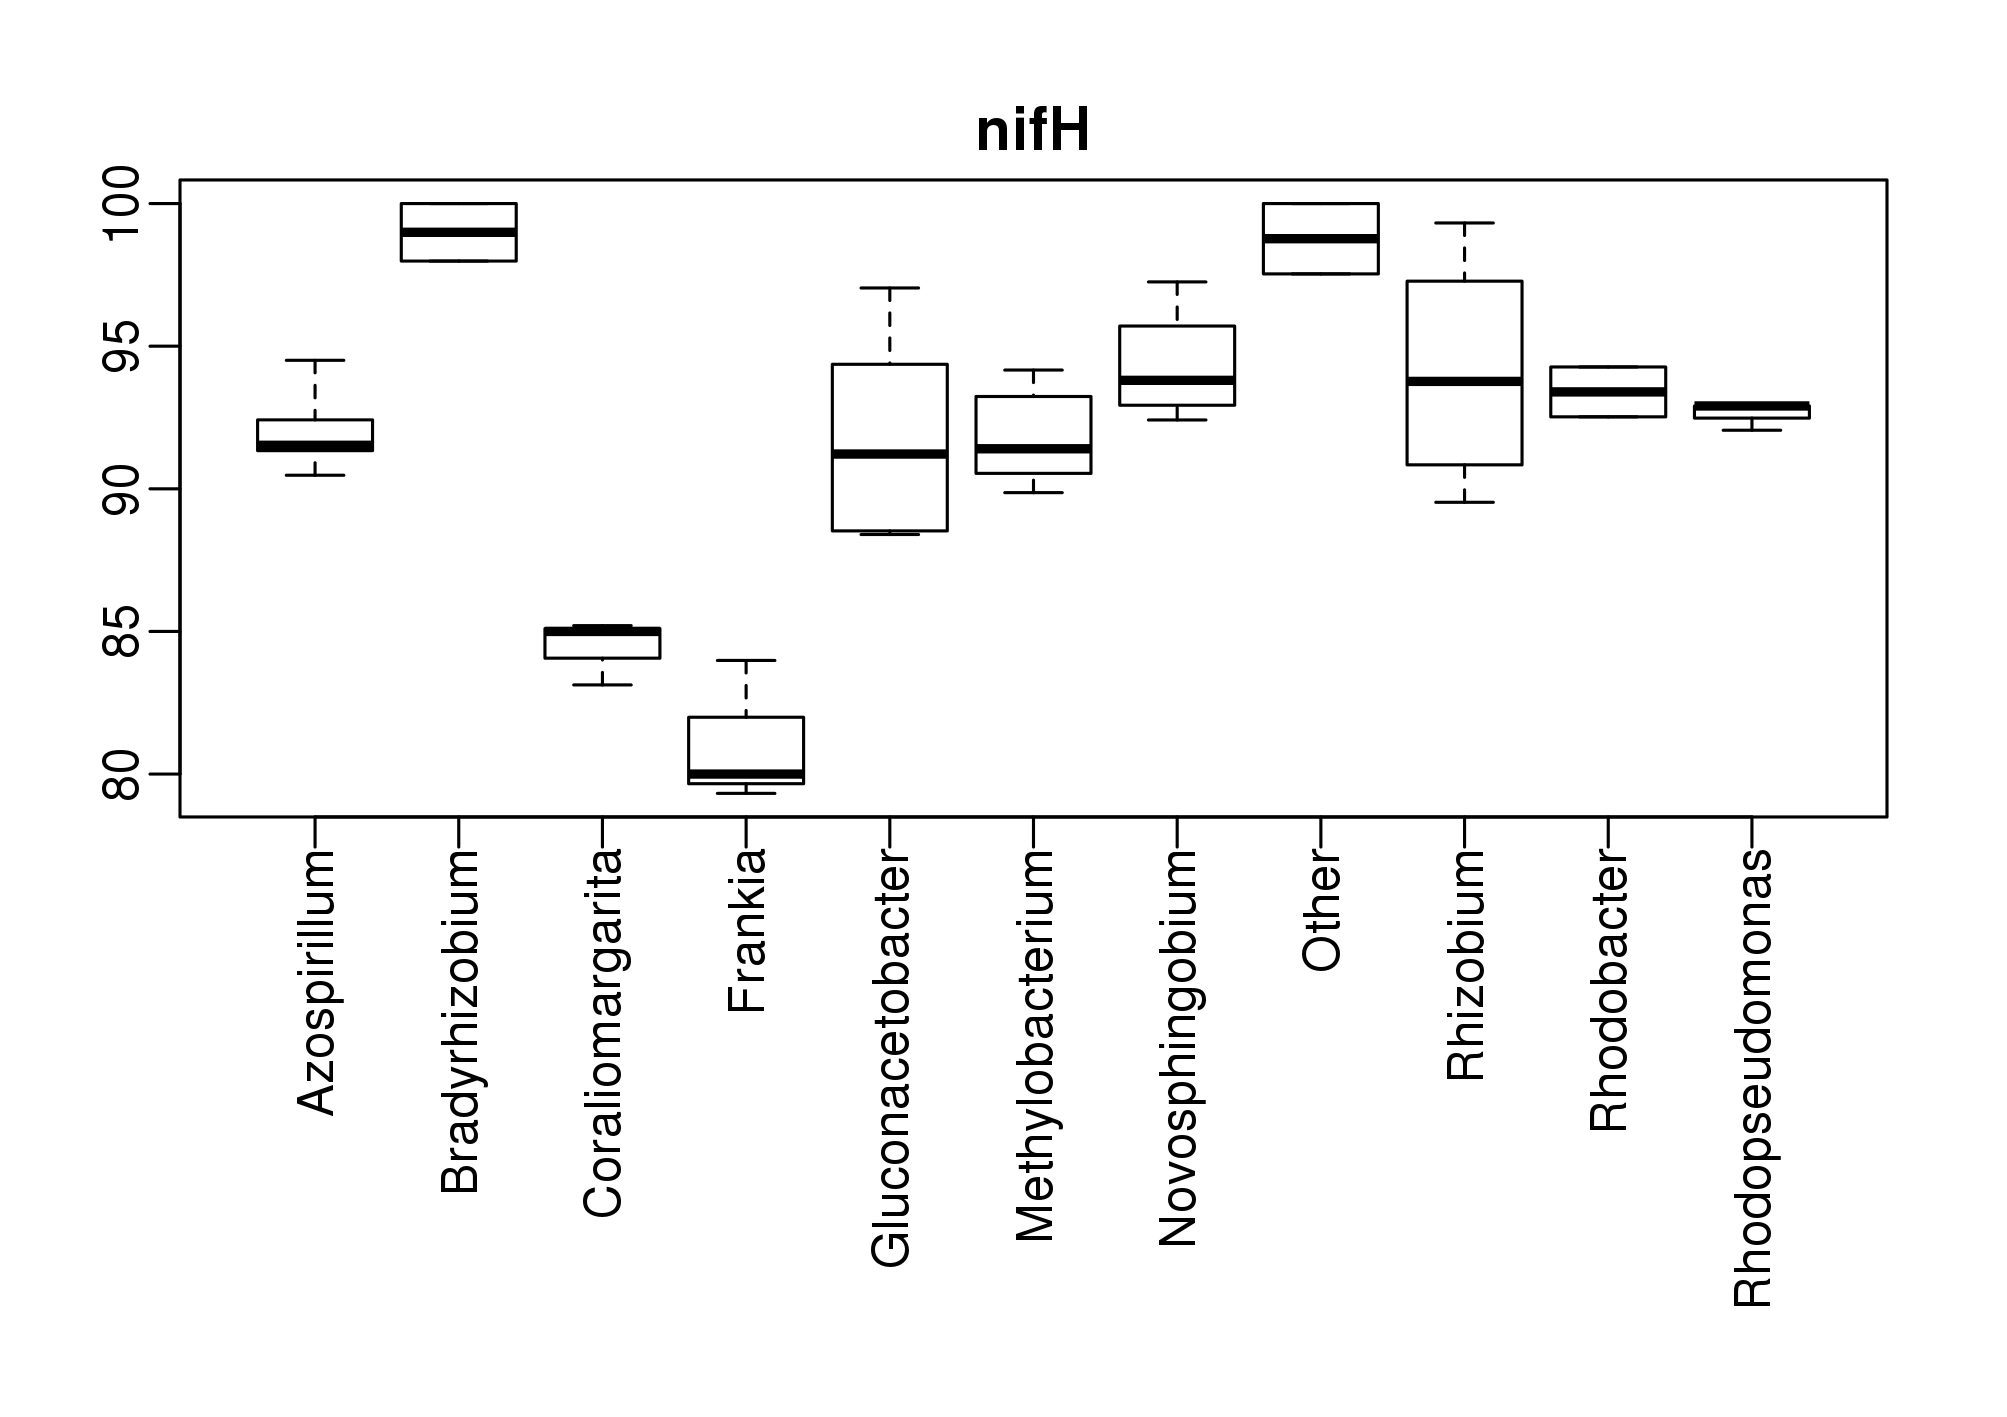
\includegraphics[scale=1]{figs/chap4-xander-nifH-genus-similarity}
  \caption[Identity of assembled nifH sequences to their best-hit references]{Distribution of identity of assembled nifH sequences to their best-hit references. Percent identities (Y axis) are grouped by genera. Assemblies with best-hit reference from Coraliomargarita and Frankia has percentage identity lower than other genera (< 85\%), indicates these sequences are more likely to be incorrectly classified.}
  \label{fig:chap4FigS10}
\end{figure}

\textbf{Metadata. }
Soil chemistry test showed higher NO3- and NH4+ in corn and no significant difference in SOM (Soil Organic Matter) and pH among soil shook off from three crops before collecting rhizosphere soil (Table \ref{tab:chap4TabS6}). Fold change of yield in 2012 over 2011 was significantly (p < 0.01, n = 5) lower in corn (more affected by drought) than perennials (\cref{fig:chap4FigS11} A). N2O flux was higher in corn on average but not significant at $\alpha = 0.05$ level due to large variation in corn and negative values caused by low flux at sampling season (\cref{fig:chap4FigS11} B).


\begin{table}[htbp]
  \centering
  \caption[Soil chemistry test results for 21 samples]{Soil chemistry test results for 21 samples.}
    \begin{tabular}{|lcccccccc|}
    \toprule
    \multicolumn{1}{|c}{\textbf{Sample ID}} & \textbf{NO3} & \textbf{NH4} & \textbf{\% OM} & \textbf{Zn} & \textbf{Mn} & \textbf{Cu} & \textbf{Fe} & \textbf{pH} \\
          & ppm   & ppm   &       & ppm   & ppm   & ppm   & ppm   &  \\
    \midrule
    C1    & 7.8   & 3.0   & 3.1   & 2.7   & 47.0  & 2.1   & 36.3  & 6.1 \\
    C2    & 1.7   & 3.4   & 2.8   & 1.9   & 36.0  & 1.5   & 28.7  & 5.7 \\
    C3    & 11.5  & 5.5   & 3.2   & 2.7   & 46.1  & 2.8   & 29.1  & 6.1 \\
    C4    & 4.7   & 3.0   & 3.3   & 2.9   & 42.5  & 2.6   & 22.3  & 6.2 \\
    C5    & 18.3  & 6.0   & 3.9   & 2.9   & 50.5  & 2.0   & 22.2  & 6.1 \\
    C6    & 4.6   & 5.5   & 3.9   & 3.1   & 38.8  & 2.6   & 27.4  & 6.2 \\
    C7    & 6.4   & 3.9   & 3.5   & 2.8   & 40.6  & 3.1   & 27.6  & 6.2 \\
    S1    & 1.2   & 3.6   & 3.6   & 2.3   & 32.0  & 2.1   & 21.5  & 6.2 \\
    S2    & 3.4   & 3.1   & 3.5   & 2.5   & 33.9  & 1.7   & 20.3  & 6.4 \\
    S3    & 2.7   & 3.1   & 4.0   & 2.9   & 34.2  & 2.7   & 25.0  & 6.2 \\
    S4    & 3.8   & 4.0   & 4.0   & 2.7   & 58.2  & 3.0   & 20.4  & 6.2 \\
    S5    & 1.1   & 2.9   & 4.9   & 3.1   & 56.3  & 3.1   & 22.9  & 6.1 \\
    S6    & 2.9   & 2.9   & 3.5   & 1.9   & 22.7  & 2.8   & 31.2  & 6.5 \\
    S7    & 1.1   & 3.1   & 3.6   & 2.2   & 27.0  & 2.3   & 28.1  & 6.1 \\
    M1    & 7.3   & 4.2   & 3.7   & 2.6   & 58.5  & 3.1   & 23.5  & 6.1 \\
    M2    & 2.4   & 4.9   & 3.5   & 1.8   & 34.5  & 3.6   & 25.0  & 5.8 \\
    M3    & 3.6   & 3.3   & 3.7   & 2.4   & 43.4  & 2.2   & 20.8  & 6.0 \\
    M4    & 1.5   & 3.2   & 3.9   & 3.1   & 48.6  & 3.1   & 25.5  & 6.0 \\
    M5    & 3.1   & 3.7   & 3.8   & 2.7   & 30.5  & 3.1   & 22.3  & 6.2 \\
    M6    & 2.1   & 4.8   & 4.3   & 3.5   & 51.9  & 3.3   & 23.8  & 6.2 \\
    M7    & 1.6   & 3.7   & 3.4   & 2.3   & 30.1  & 2.7   & 22.9  & 6.5 \\
    \bottomrule
    \end{tabular}%
  \label{tab:chap4TabS6}%
\end{table}%

\begin{figure}[tbph!]
  \centering
  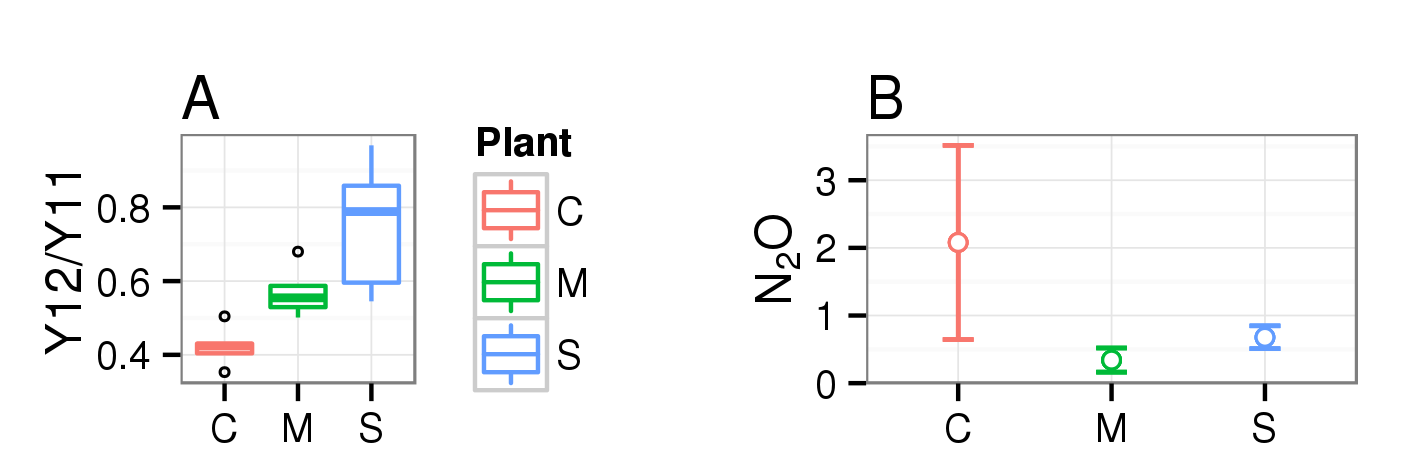
\includegraphics[scale=1]{figs/chap4-meta-n2o-yield-ratio}
  \caption[Ratio of 2012 yield over 2011 and N2O flux]{Ratio of 2012 yield over 2011 and N2O flux measured near sampling time. Ratio of 2012 yield over 2011 of corn is significantly lower than Miscanthus and switchgrass, suggesting corn yield is impacted more by 2012 drought (A). Average of N2O flux is higher in corn than Miscanthus and switchgrass, but not significant at $\alpha = 0.05$ level due to high variation in corn (B).}
  \label{fig:chap4FigS11}
\end{figure}


\section{Discussion}

In this study, we apply shotgun metagenomics to investigate rhizosphere microbial community structure and function of three biofuel crops (corn, Miscanthus, and switchgrass), with a focus on N cycle genes. We find corn is the most different among three crops, in community structure (\ref{fig:chap4Fig1} A), assembled genomic sequences (Table \ref{tab:chap4TabS3}), and functional profile (\ref{fig:chap4Fig1} C). It is expected that different plants have different rhizosphere microbial communities \cite{smalla_bulk_2001,mao_changes_2011}, but our comparative metagenomic analyses of assemblies and functional profile is beyond the existing studies relying on 16S rRNA gene or a few other functional genes \cite{mao_changes_2011,mao_impact_2013}. Metagenome assembly could represent genomic content of communities and thus genetic diversity. Species diversity, genetic diversity, and functional diversity all show corn has significantly different rhizosphere microbial community than perennials (\cref{fig:chap4Fig1} A and C, Table \ref{tab:chap4TabS3}), suggesting that change of biofuel crop in large scale can impact microbial communities and ecosystem services.

The corn rhizosphere community also shows more variation among replicates in ordination plot (\cref{fig:chap4Fig1} A). In contrary, community turnover within replicates (beta diversity) based on number of unique OTUs is similar among three crops (\cref{fig:chap4FigS2}), so the larger dispersion in corn is probably caused by variation in abundance of shared OTUs. There are two possible explanations: First, corn is annual and grows from seeds and establish its root system every year, while perennials (Miscanthus and switchgrass) have more stable root systems that influence microbial community in rhizosphere. As a result, rhizosphere microbial communities of corn show more stochasticity. Second, corn has been bred for grain yield under intensive management (e.g. fertilization) for a long time and some traits for recruiting beneficial microbiome may have been lost. Thus larger variation of corn rhizosphere community may suggest weaker influence and selection from corn roots.


\begin{figure}[tbph!]
  \centering
  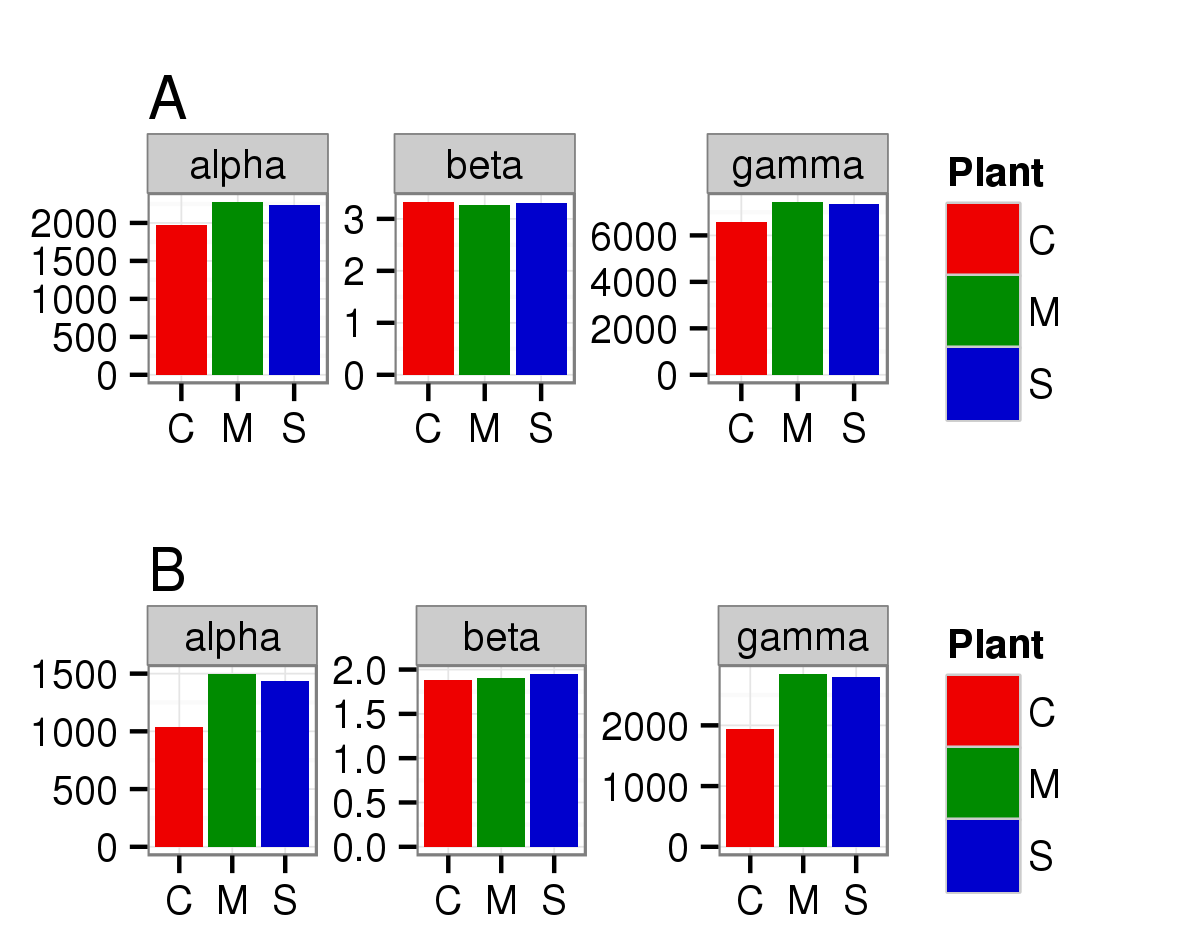
\includegraphics[scale=1]{figs/chap4-otu-alpha-beta-gamma-trudiv}
  \caption[Species (OTU) diversity of three crops]{Species (OTU) diversity of three crops. Miscanthus and switchgrass are higher in both observed OTU number (q = 0 for ``trudiv'' function in simba package in R) (A) and another diversity index (B, q = 1 for ``trudiv'' function) (B). C stands for corn, M stands for Miscanthus and S stands for switchgrass. Alpha (diversity) refers to diversity of each replicate, gamma (diversity) refers to diversity when all replicates of each crop are combined, and beta (diversity) is ratio of gamma over alpha.}
  \label{fig:chap4FigS2}
\end{figure}

In spite of the larger dispersion in corn, perennials have higher alpha (local) diversity and also gamma diversity (when replicates are combined by plant) (\cref{fig:chap4FigS2}). Thus change from annual to perennials as biofuel crops can increase the overall microbial diversity, which could also have a significant impact on ecosystem. According to a study on disturbance and diversity models \cite{svensson_disturbance-diversity_2012}, evenness should increase when disturbance are introduced. Corn has to re-grow roots every year, which could be considered as a regular disturbance. The annual life cycle of corn should encourage a more even community, which contradicts to our result that corn is less even than perennials. Thus the lower evenness of corn rhizosphere community should be attributed to root exudates, root detritus (especially for corn), or agricultural management (e.g. fertilize), which are further discussed below.

Consistent with diversity, there are also significant difference in taxonomy composition between corn and the other two perennial crops. Proteobacteria enriched in corn are commonly considered to be copiotrophic taxa and acidobacteria enriched in perennials are oligotrophic taxa \cite{fierer_toward_2007,eilers_shifts_2010}. Increased N input can cause a shift from oligotrophic to copiotrophic taxa \cite{fierer_comparative_2012,wessen_differential_2010}. Thus more copiotrophic taxa in corn can be explained by higher N fertilizer usage and higher N found in rhizosphere soil (Table \ref{tab:chap4TabS6}). Further, since copiotrophs need more carbon as well nitrogen, we predict that corn is also providing more carbon source (root exudate and detritus) compared to perennials, which is consistent with more ``Carbohydrates'' related pathway genes enriched in corn rhizosphere shown in functional diversity analysis (\cref{fig:chap4FigS5}). Since copiotrophs have relatively faster growth rate in nutrient rich environment \cite{fierer_comparative_2012}, they outnumbered the rest, which explains the lower evenness in corn mentioned above (\cref{fig:chap4FigS3}).

Additionally, the higher fungal-to-bacterial ratio in corn also suggests corn provides more carbon source to the rhizosphere compared to perennials and encourages copiotrophic bacteria, which is consistent with the above. Higher fungal-to-bacterial ratio commonly indicates higher C/N ratio since fungal biomass has higher C/N ratio than bacteria \cite{de_vries_fungal/bacterial_2006,waring_differences_2013}. Due to the fact that fungi has larger biomass to DNA ratio than bacteria (some fungal hyphae may not have nuclei) and fungal DNA are harder to extract \cite{muller_rapid_1998}, the ratios (DNA based) here are much smaller than reported in other studies using biomass \cite{jesus_influence_2015}. Moreover, Penicillium, a commonly saprotroph but hardly known as beneficial to plants (to the best of our knowledge), is highly enriched in corn (the third most abundant genus), which suggests that corn provides more carbon source to rhizosphere but not effectively recruiting beneficial members (selecting non-beneficial ones in this case).

There is more ``Stress responses'' related pathway genes enriched in corn, which indicates rhizosphere community of corn is under more stress. Especially, the enriched ``Desiccation stress'' related genes in corn is consistent with the fact that it was a drought year in 2012 and corn production is mostly affected by the drought (\cref{fig:chap4FigS11} A). Moreover, higher number of phage and prophage related genes in corn rhizosphere also indicates that corn rhizosphere community is at higher risk of phage infection and thus unstable, consistent with lower evenness and diversity of corn rhizosphere community compared to perennials.

Our global assembly and annotation pipeline is not suitable for evaluating N cycle genes, since the annotation database that we use, SEED subsystem \cite{meyer_metagenomics_2008}, does not include any nitrification genes. Moreover, Xander provides better sensitivity and specificity, and recover longer assemblies \cite{wang_xander:_2015}. OTU based ordination analyses of all N cycle genes except AOA shows the significant separation of three crops (\cref{fig:chap4Fig3}), which is the same as SSU rRNA gene and functional profile (\cref{fig:chap4Fig1} A and C) and suggests that nitrogen fixing, nitrifying, and denitrifying community are also changed when crops are switched from corn to Miscanthus and switchgrass, consistent with the overall community, except that the separation of Miscanthus and switchgrass becomes more significant.

Perennials has more nifH than corn on average (significant for Miscanthus but not significant for switchgrass at $\alpha = 0.05$ level), suggesting perennials have more nitrogen fixing microbes, which could explain why Miscanthus and switchgrass growth does not always respond to nitrogen input \cite{schwarz_effect_1994,parrish_biology_2005} (S. Roley, unpublished data) and is consistent with another study using qPCR \cite{mao_impact_2013}. Three crops are very different in taxon composition with \textit{Rhizobium} as the most abundant in corn, \textit{Coraliomargarita} as the most abundant in Miscanthus, and \textit{Novosphingobium} as the most abundant in switchgrass (\cref{fig:chap4Fig6}), which suggests each crop is different in the nitrogen fixing members, consistent with ordination analysis using OTUs (\cref{fig:chap4Fig3}). Since these plots were planted with soybean and alfalfa before the experiment site was established, we can assume \textit{Rhizobium} was abundant before three crops were planted. Thus some Rhizobia (including \textit{Rhizobium} and \textit{Bradyrhizobium}) may stick around in corn plots due to agricultural management (N fertilizer and less root influence caused by annual life cycle) or its inability to select beneficial microbes. On the other hand, perennials can select beneficial microbes such as \textit{Coraliomargarita}, \textit{Azospirillum}, Nostoc, \textit{Novosphingobium}, and \textit{Gluconacetobacter}, which further competitively exclude Rhizobia. Further, many nitrogen fixing members in corn rhizosphere may not be active, since Rhizobia needs leguminous plant host to grow. Additionally, note that there is a lot of variation in taxon composition in replicates (\cref{fig:chap4Fig6}), but clearly there are different genera that stand out for all three crops though weak in a rep or two, which underscores the importance of replication in soil studies.

Two nitrifying groups (AOA and AOB) both have very low diversity (3 OTUs) compared to other genes (\cref{fig:chap4FigS6,fig:chap4FigS7}) and do not have significantly difference among three crops. However, AOB communities are significantly different among three crops, while AOA are not (\cref{fig:chap4Fig3}), indicating that AOB community composition are affected more than AOA when crops are changed, which is consistent with a study using amplicon methods \cite{shen_abundance_2008,wang_community_2009}. Further, the result that corn with added N fertilizer does not have the highest abundance of nitrifying members (\cref{fig:chap4Fig4}) suggests nitrifier abundance does not positively respond to N fertilizer, which may be explained by drought that caused too low soil moisture for nitrifiers \cite{di_effect_2014} and by no tillage that cause low oxygen (bad aeration) in corn rhizosphere. Conversely, perennials have less affected by the drought due to their deeper and larger root systems.

Denitrification has multiple steps (nitrite reduction, nitric oxide reduction, and nitrous oxide reduction included our analysis) and each step has more than one gene coding enzymes with same function for the same process, which makes it difficult to draw any conclusion when comparing three crops. For example, nirK is significantly higher in corn but nirS is not significantly different among three. Thus we combined those genes coding enzymes with the same function, which leads to the finding that there are significantly more nitrite reductase genes but less nitric oxide reductase genes and nitrous oxide reductase genes in corn (\cref{fig:chap4Fig5}). Since nitrite reduction is considered as the rate limiting step in denitrification chemistry \cite{zumft_cell_1997} and the abundance of nitrite reduction genes are significantly lower than downstream steps including nitric oxide reduction and nitrous oxide reduction (\cref{fig:chap4Fig5}), corn have higher overall denitrification potential, which is consistent with more N fertilizer input in corn (higher substrate availability) and higher average N2O flux in corn (\cref{fig:chap4FigS11} B) \cite{oates_nitrous_2015}.

Other than community structure and function comparison among three crops, we also have some general findings about rhizosphere soil at our sampling site. First, ammonia-oxidizing archaea are about three times more abundant than ammonia-oxidizing bacteria on average, consistent with other studies \cite{leininger_archaea_2006,prosser_archaeal_2012,gubry-rangin_archaea_2010}. Bacteria with nirK type nitrite reductase are about nine times more abundant than those with nirS. Bacteria with qNor type nitric oxide reductase are 14 times more abundant than those with cNor. Bacteria with nosZa2 are four times more abundant than nosZ (\cref{fig:chap4FigS8}). The above ratios also suggest that traditional amplicon studies that only target one gene in those processes might get misleading conclusions, e.g. nosZ of nitrous reduction is the higher in corn but nosZa2 is the higher in Miscanthus and switchgrass. Second, nitrogen fixing bacteria are about 0.4\% of total community on average; nitrifiers are about 1.4\% on average; denitrifier are about 10.6\%, 22.4\% and 15.6\% of total community for nitrite reduction, nitric oxide reduction, and nitrous oxide reduction respectively (\cref{fig:chap4Fig4,fig:chap4Fig5}). Both the above ratios and abundance are valuable information for future studies of this sampling site.

Another contribution of this study is that we find whole N cycle genes that are distant from existing references (\cref{fig:chap4FigS9}), which can help improve primer design of these genes. Further, since taxon assignment is done by best hit reference sequence, taxonomy information of the assembled N cycle gene may be not correct (especially for those with low identity), but that’s the best we can do based on limiting reference sequences. It is also worth mentioning that the most abundant group of assembled nifH sequences (those assigned to the most abundant genus \textit{Coraliomargarita}) in Miscanthus have identity of only about 85\% to best hit reference (\cref{fig:chap4FigS10}), even though nifH is the most studied N cycle gene.

\section{Conclusion}

In this study, we showcase the power of shotgun metagenomics to study microbial ecology at both community structure and function levels. We sequenced about 1 TB of rhizosphere metagenome, which is one of the largest sequencing efforts on rhizosphere soil and enables us to study functional traits that are not abundant. Overall community structure (SSU rRNA gene), overall function (annotation from global assembly), and N cycle genes (except AOA) all show corn has significantly different community from Miscanthus and switchgrass, suggesting changing bioenergy crop from corn (annual) to Miscanthus and switchgrass (perennial) will have impact on ecosystem functions carried out by microbiome. Further, we find corn have less influence and selection on its rhizosphere community, supported by larger variation in community composition, enriched Penicillium (non-beneficial fungi), and predominance of \textit{Rhizobium} and \textit{Bradyrhizobium} (left from before establishing the study site). Further, perennials manage to maintain more diverse microbial communities in rhizosphere by investing less carbon source (root detritus and exudate). Moreover, we find perennials have more N fixing genes (nifH) and nitrite reducing genes (sum of nirK and nirS), which agrees with better N sustainability of Miscanthus and switchgrass \cite{schwarz_effect_1994,parrish_biology_2005}. Thus perennials bioenergy crops have advantage over corn in maintain microbial species and functional diversity and also selecting members with beneficial traits.


%\appendix
%\chapter{Your appendix}
%
\backmatter
% The next lines add the dots back into the References/Bibliography heading
% of the TOC.  Only uncomment this if you need to put the dots back in having removed them for Chapter headings.
%
%\addtocontents{toc}{%
%   \protect\renewcommand{\protect\cftchapterdotsep} {\cftdotsep}}
%
\makebibliographypage % make the bibliography cover page
% Bibliography can be single spaced
%
\SingleSpacing
%
% Your bibliography command here (e.g. \bibliography{your-bib-file}) if using natbib
%
\bibliographystyle{unsrt}
\bibliography{main}

% Remember that although the bibliography is single spaced, there needs to
% be a blank line between entries. This is set by your bibliography package
% If you are using natbib it is \bibsep; if using biblatex it's \bibitemsep
\end{document}

